\documentclass[12pt]{thesul}
%----------------------------------------------------------------------
%                               Packages
%----------------------------------------------------------------------
\usepackage[french]{babel}
\usepackage{acronym} % \ac[p], \acl[p], \acs[p], \acf[p]
\usepackage{biblatex}
\bibliography{biblio.bib}
\usepackage{booktabs} % \toprule, \midrule, \cmidrule, \bottomrule
\usepackage{caption}
\usepackage{csquotes}
\usepackage{hyperref}
\hypersetup{hidelinks}
\usepackage[inline]{enumitem}
\usepackage[french]{minitoc}

\usepackage{xcolor}
\AtBeginDocument{
\definecolor{pdfurlcolor}{rgb}{0,0,0}
\definecolor{pdfcitecolor}{rgb}{0,0,0}
\definecolor{pdflinkcolor}{rgb}{0,0,0}
\definecolor{light}{gray}{.85}
\definecolor{vlight}{gray}{.95}
\definecolor{darkgreen}{RGB}{77,172,38}
\definecolor{darkblue}{RGB}{5,113,176}
\definecolor{mydarkblue}{RGB}{116,173,209}
\definecolor{mydarkblueid}{RGB}{83,154,198}
\definecolor{mylightblue}{RGB}{171,217,233}
\definecolor{mydarkorange}{RGB}{244,109,67}
\definecolor{mylightorange}{RGB}{252,153,54}
\definecolor{mydarkred}{RGB}{215,48,39}
\definecolor{mydarkpurple}{RGB}{140,107,177}
\definecolor{mydarkpurpleid}{RGB}{136,86,167}
}

\usepackage{amssymb}
\usepackage{amsmath}
\interdisplaylinepenalty=2500
\newtheorem{definition}{Définition}
\newtheorem{myrule}{Règle}
\newtheorem{property}{Propriété}
\newtheorem{subproperty}{Propriété}[property]

\usepackage{algorithm, algpseudocode}
\floatname{algorithm}{Algorithme} % Renomme caption de "Algorithm" -> "Algorithme"

\usepackage[draft,inline,nomargin,index]{fixme}
\fxsetup{theme=color,mode=multiuser,inlineface=\itshape,envface=\itshape}
\FXRegisterAuthor{go}{ago}{Gerald}
\FXRegisterAuthor{mn}{amn}{Matthieu}

\usepackage{tikz} % \begin{tikzpicture} \end{tikzpicture}
\usetikzlibrary{calc}
\usetikzlibrary{graphs}
\usetikzlibrary{quotes}
\usetikzlibrary{shapes.misc}

\usepackage[caption=false,font=footnotesize,labelfont=sf,textfont=sf]{subfig}

% Commands
%---------
\newcommand{\eg}{e.g. }
\newcommand{\ie}{c.-à-d. }

\newcommand{\headerparagraph}[1]{\textbf{\emph{#1}}\quad}

\newcommand{\inbb}[1]{\in \mathbb{#1}}
\newcommand{\mathlist}[2]{\set{#1_i \in #2}_{i \inbb{N}}}
\newcommand{\new}{\textbf{new}}
\newcommand{\trm}[1]{\mathit{#1}}
\newcommand{\set}[1]{\left\{#1\right\}} % set brace notation

\newcommand{\id}[3]{$\trm{#1}^{\trm{#2}}_{\trm{#3}}$}
\newcommand{\epoch}[1]{$\varepsilon_{#1}$}
\newcommand{\lid}{$<_{id}$~}
\newcommand{\leqid}{$\leq_{id}$~}
\newcommand{\lepoch}{$<_{\varepsilon}$~}
\newcommand{\leqepoch}{$\leq_{\varepsilon}$~}

\newcommand\bigO[1]{$\mathcal{O}(#1)$}

\newcommand{\widthletter}{2em}
\newcommand{\widthblock}{3em}
\newcommand{\widthoriginepoch}{1.33em}
\newcommand{\widthepoch}{1.65em}

% Définit noms pour \autoref
%---------
\newcommand{\algorithmautorefname}{Algorithme}
\newcommand{\annexautorefname}{Annexe}
\newcommand{\definitionautorefname}{Définition}
\newcommand{\propertyautorefname}{Propriété}
\newcommand{\subfigureautorefname}{Figure}
\newcommand{\subpropertyautorefname}{Propriété}

% Tikz styles
\tikzset{
    common/.style={anchor=west, draw, rectangle, minimum height=6mm},
    letter/.style={common, minimum width=\widthletter},
    block/.style={common, minimum width=\widthblock},
    epoch/.style={letter, rounded rectangle, rounded rectangle east arc=0pt, minimum width=\widthepoch},
    point/.style={insert path={ node[scale=5*sqrt(\pgflinewidth)]{.} }},
    op/.style={draw, circle, minimum size=2.7em},
    causalop/.style={op, double=white, inner sep=2pt},
    gc-rule-1/.style={dashed, thick, darkblue},
    gc-rule-2/.style={densely dotted, thick, darkgreen},
    cross/.style={
        path picture={
            \draw[mydarkred, very thick]
                (path picture bounding box.south east)--(path picture bounding box.north west)
                (path picture bounding box.south west)--(path picture bounding box.north east);
        }
    }
}


%-------------------------------------------------------------------
%                             Marges
%-------------------------------------------------------------------

% pour positionner les vraies marges:
%\SetRealMargins{1mm}{1mm}

%-------------------------------------------------------------------
%                             En-têtes
%-------------------------------------------------------------------

% Les en-têtes: quelques exemples
%\UppercaseHeadings
%\UnderlineHeadings
%\newcommand\bfheadings[1]{{\bf #1}}
%\FormatHeadingsWith{\bfheadings}
%\FormatHeadingsWith{\uppercase}
%\FormatHeadingsWith{\underline}
\newcommand\upun[1]{\uppercase{\underline{\underline{#1}}}}
\FormatHeadingsWith\upun

\newcommand\itheadings[1]{\textit{#1}}
\FormatHeadingsWith{\itheadings}

% pour avoir un trait sous l'en-tete:
\setlength{\HeadRuleWidth}{0.4pt}

%-------------------------------------------------------------------
%                         Les références
%-------------------------------------------------------------------

\NoChapterNumberInRef
\NoChapterPrefix

%-------------------------------------------------------------------
%                           Brouillons
%-------------------------------------------------------------------

% ceci ajoute une marque « brouillon » et la date
\ThesisDraft

%-------------------------------------------------------------------
%                   Pour collecter un glossaire et un index
%-------------------------------------------------------------------

\makeglossary
\makeindex

%-------------------------------------------------------------------
%                           Acronymes
%-------------------------------------------------------------------

% Acronyms
% --------
% \input{assets/acronyms.tex}
\acrodef{ADT}[ADT]{Abstract Data Type}
\acrodefplural{ADT}[ADTs]{Abstract Data Types}
\acrodef{API}[API]{Application Programming Interface}
\acrodef{CRDT}[CRDT]{Conflict-free Replicated Data Type}
\acrodefplural{CRDT}[CRDTs]{Conflict-free Replicated Data Types}
\acrodef{FIFO}[FIFO]{First In, First Out}
\acrodef{JIT}[JIT]{Just-In-Time}
\acrodef{LCA}[PPAC]{Plus Petit Ancêtre Commun}
\acrodef{MUTE}[MUTE]{Multi User Text Editor}
\acrodef{OT}[OT]{Operational Transformation}
\acrodefplural{OT}[OT]{Operational Transformations}
\acrodef{P2P}[P2P]{Pair-à-Pair}
\acrodef{PKI}[PKI]{Public Key Infrastructure}
\acrodef{SEC}[SEC]{Cohérence forte à terme}
\acrodef{WebRTC}[WebRTC]{Web Real-Time Communication}

%-------------------------------------------------------------------
%                           Couleurs
%-------------------------------------------------------------------

% \input{assets/colours.tex}

%-------------------------------------------------------------------
%                     Global custom tikz commands
%-------------------------------------------------------------------

% \input{assets/tikz_presets.tex}

\begin{document}


      \OddHead={{\leftmark\rightmark}{\hfil\slshape\rightmark}}
      \EvenHead={{\leftmark}{{\slshape\leftmark}\hfil}}
      \OddFoot={\hfil\thepage}
      \EvenFoot={\thepage\hfil}
      \pagestyle{ThesisHeadingsII}


%-------------------------------------------------------------------
%                          Encadrements
%-------------------------------------------------------------------

% encadre les chapitres dans la table des matières:
% (ces commandes doivent figurer apres \begin{document}

\FrameChaptersInToc
%\FramePartsInToc


%-------------------------------------------------------------------
%            Réinitialisation de la numérotation des chapitres
%-------------------------------------------------------------------

% Si la commande suivante est présente,
% elle doit figurer APRÈS \begin{document}
% et avant la première commande \part
\ResetChaptersAtParts

%-------------------------------------------------------------------
%               mini-tables des matières par chapitre
%-------------------------------------------------------------------

% préparer les mini-tables des matières par chapitre.
% (commande de minitoc.sty)
\dominitoc

%-------------------------------------------------------------------
%                         Page de titre:
%-------------------------------------------------------------------

\ThesisTitle{Ré-identification efficace dans les types de données répliquées sans conflit (CRDTs)}
\ThesisDate{TODO: Définir une date}
\ThesisAuthor{Matthieu Nicolas}

% Type de la these
\ThesisUL
% Jury:

% (ne pas mettre de \\ apres la dernière entree)

% Exemple de création d'une nouvelle catégorie dans le jury:

\NewJuryCategory{family}{\it Membre de la famille :}
                        {\it Membres de la famille :}

\family={Mon frère\\Ma sœur}

\def\blanc{\hspace*{1cm}}

\President    = {Stephan Merz}
\Rapporteurs  = {Le rapporteur 1&de Paris\\
                 Le rapporteur 2\\
                 \blanc suite&taratata\\
                 Le rapporteur 3}
\Examinateurs = {L'examinateur 1&d'ici\\
                 L'examinateur 2}
%\Invites=       {}

% Création de la page de titre:
\MakeThesisTitlePage

%-------------------------------------------------------------------


%-------------------------------------------------------------------
%                          remerciements
%-------------------------------------------------------------------

%\DontFrameThisInToc
\begin{ThesisAcknowledgments}
Les remerciements.
\end{ThesisAcknowledgments}

%-------------------------------------------------------------------
%                            dédicace
%-------------------------------------------------------------------

\begin{ThesisDedication}
Je dédie cette thèse\\
à ma machine.\\
Oui, à Pandore,\\
qui fut la première de toutes.
\end{ThesisDedication}


%-------------------------------------------------------------------
%                  écriture de `Chapitre' et `Partie'
%                      dans la table des matières
%-------------------------------------------------------------------

\WritePartLabelInToc
\WriteChapterLabelInToc

%-------------------------------------------------------------------
%                        table des matières
%-------------------------------------------------------------------

\tableofcontents

%-------------------------------------------------------------------
%              Exemple d'utilisation de \SpecialSection
%-------------------------------------------------------------------
%\SpecialSection{Introduction générale}

\DontWriteThisInToc
\listoffigures

\mainmatter
\NumberThisInToc
\chapter*{Introduction}
\minitoc
\section{Contexte}
\section{Questions de recherche}
\section{Contributions}
\section{Plan du manuscrit}
% Dans ce chapitre, nous revenons sur les contributions présentées dans cette thèse.
Nous rappelons le contexte dans lequel elles s'inscrivent, récapitulons leurs spécificités et apports, et finalement précisons plusieurs de leurs limites.
Puis, nous concluons ce manuscrit en présentant plusieurs pistes de recherche qui nous restent à explorer à l'issue de cette thèse.
La première s'inscrit dans la continuité directe de nos travaux sur un mécanisme de ré-identification pour \acp{CRDT} pour le type Séquence pour les applications \acf{LFS}.
Les dernières traduisent quant à elles notre volonté de recentrer nos travaux sur le domaine plus général des \acp{CRDT}.


% \NumberThisInToc
% \chapter*{Problématique}
% \minitoc
% \input{assets/chapter_problematic}

\NumberThisInToc
\chapter{État de l'art}
\minitoc

\section{Systèmes distribués}

\begin{itemize}
  \item Contexte des systèmes distribués à large échelle
  \item Réplique les données afin de pouvoir supporter les pannes
  \item Adopte le paradigme de la réplication optimiste \cite{10.1145/1057977.1057980}
  \item Autorise les noeuds à consulter et à modifier la donnée sans aucune coordination entre eux
  \item Autorise alors les noeuds à diverger temporairement
  \item Permet d'être toujours disponible, de toujours répondre aux requêtes même en cas de partition réseau
  \item Permet aussi, en temps normal, de réduire le temps de réponse (privilégie la latence) \cite{pacelc2012}
  \item Comme ce modèle autorise les noeuds à modifier la donnée sans se coordonner, possible d'effectuer des modifications concurrentes
  \item Généralement, un mécanisme de résolution de conflits est nécessaire afin d'assurer la convergence des noeuds dans une telle situation
  \item Plusieurs approches ont été proposées pour implémenter un tel mécanisme
\end{itemize}

\section{Transformées opérationnelles}

\begin{itemize}
  \item Approche permettant de gérer des modifications concurrentes sur un type de données
  \item Consiste à transformer les opérations par rapport aux effets des opérations concurrentes pour rendre les rendre commutatives.
    Permet de rendre l'ordre d'intégration des opérations sans importance par rapport à l'état final obtenu
  \item Se décompose en 2 parties : algorithmes (génériques) et fonctions de transformations (spécifiques au type de données)
  \item Plusieurs algorithmes OT adoptent une architecture centralisée (trouver citations)
  \item Cette architecture pose des problèmes de performances (bottleneck), sécurité (SPOF), coût, d'utilisabilité (mode offline), pérennité (disparition du service), vie privée et de résistance à la censure.
  \item Pour ces raisons, des algorithmes reposant sur une architecture décentralisée ont été proposés
  \item Mais ne règlent qu'en partie ces limites
  \item Notamment, ne sont pas adaptés à des systèmes P2P dynamiques
  \item Besoin de vector clocks sur chaque opération pour détecter la concurrence.
    Vector clocks adaptés dans systèmes à nombre de pairs fixe, mais pas aux systèmes dynamiques (revoir causal barrier pour p-e nuancer ce propos).
  \item Néanmoins, cette approche a permis de démocratiser les systèmes collaboratifs via son adoption par des services tels que Google Docs, Overleaf, Framapad
  \item De plus, dans le cadre de ces travaux, ont été définies les propriétés CCI \cite{10.1145/274444.274447}.
  \item Remettre en question la propriété Causalité des CCI.
    Généralement, confond causalité et happen-before et exprime en finalité une contrainte trop forte.
    Cette contrainte peut réduire la réactivité du système (exemple avec 2 insertions sans liens mais qui force d'attendre la 1ère pour intégrer la 2nde).
    Causalité pose aussi des problèmes de passage à l'échelle car repose sur vector clocks.
    IMO, doit relaxer cette propriété pour pouvoir construire systèmes à large échelle.
\end{itemize}

\mnnote{TODO: Mentionner TP1 et TP2}

\mnnote{TODO: Spécification faible et forte des séquences répliquées}

\section{Séquences répliquées sans conflits}
\subsection{Types de données répliquées sans conflits}
\subsubsection{Principes}

\begin{itemize}
  \item Nouvelles spécifications des types de données existants
  \item Structures conçues pour être répliquées au sein d'un système
  \item Et être modifiées sans coordination par ses différents noeuds
  \item Doivent donc supporter de nouveaux scénarios uniquement possible dans des exécutions parallèles
  \item Et définir une sémantique pour ces scénarios inédits
  \begin{itemize}
    \item Exemple du Registre avec LWW-Register et MV-Register ?
  \end{itemize}
  \item Pour gérer ces scénarios, intègrent un mécanisme de résolution de conflits directement au sein de leur spécification
  \item Garantissent la cohérence forte à terme
  \item \mnnote{
      TODO: Lister les CRDTs ayant été proposés.
      Registre, Ensemble, Sequence, Graphe, JSON, Filesystem, Access Control
    }
\end{itemize}

\mnnote{Faire le lien avec les travaux de Burckhardt \cite{10.1145/2535838.2535848} et les MRDTs \cite{10.1145/3360580}}

\subsubsection{Familles de types de données répliquées sans conflits}

\begin{itemize}
  \item Une catégorisation des CRDTs a été proposée
  \item Propose de répartir les CRDTs en différentes familles en fonction de la méthode de synchronisation utilisée
  \item Chacune de ces méthodes de synchronisation implique des contraintes sur la couche réseau du système et entraîne des répercussions sur la structure de données elle-même
  \item Types de données répliquées sans conflits à base d'états \cite{shapiro_2011_crdt, shapiro:inria-00555588}
  \begin{itemize}
    \item Les noeuds partagent leur état de manière périodique
    \item Une fonction \emph{merge} permet aux noeuds de fusionner leur état courant avec un autre état reçu
    \item Aucune hypothèse sur la partie réseau autre que les noeuds arrivent à communiquer à terme
    \item Pas un problème si états perdus, les prochains intégreront les informations de ces derniers
    \item Pas un problème si états reçus dans le désordre, la fonction \emph{merge} est commutative
    \item Pas un problème si états reçus plusieurs fois, \emph{merge} est idempotent
    \item Mais nécessite de conserver au sein de la structure de données assez d'informations pour proposer une telle fonction de \emph{merge}
    \item Par exemple, besoin de conserver une trace des éléments supprimés pour empêcher leur réapparition suite à une fusion d'états
    \item \mnnote{TODO: Ajouter forces, faiblesses et cas d'utilisation de cette approche}
  \end{itemize}
  \item Types de données répliquées sans conflits à base d'opérations \cite{shapiro_2011_crdt, shapiro:inria-00555588, 2014-making-op-based-crdts-op-based, baquero2017pure}
  \begin{itemize}
    \item Les noeuds partagent uniquement des opérations représentant leurs modifications
    \item Une modification peut se formaliser en deux étapes
    \item \emph{prepare}, qui permet de générer une opération correspondant à une modification
    \item \emph{effect}, qui permet d'appliquer l'effet de la modification à un état
    \item Les opérations concurrentes doivent être commutatives pour assurer la convergence
    \item Mais pas de contraintes sur les opérations causalement liées
    \item Pas de contraintes non plus sur l'idempotence des opérations
    \item Nécessite donc généralement d'ajouter une couche \emph{livraison} pour faire le lien entre le réseau et le CRDT
    \item Permet d'attacher des informations de causalité aux opérations locales avant de les envoyer
    \item Permet de ré-ordonner et filtrer les opérations distantes reçues avant de les fournir au CRDT
    \item Besoin d'un mécanisme d'anti-entropie \cite{1983-anti-entropy-vv} pour assurer que l'ensemble des noeuds observent l'ensemble des opérations et ainsi garantir la convergence
      \mnnote{TODO: Ajouter référence mécanisme d'anti-entropie basé sur Merkle Tree}
    \item Généralement, impose que la couche livraison soit compliant avec Reliable Causal Broadcast
    \item Mais s'agit dans plusieurs cas d'une contrainte plus forte que nécessaire
      \mnnote{
        TODO: Me semble que c'est \cite{baquero2017pure} qui indique la nécessité de RCB.
        Relire si c'est vraiment le cas pour les CRDTs qu'il présente dans le papier.
      }
    \item Opérations permettent de lisser la consommation réseau
    \item Et offrent des temps d'intégration et de propagation des modifications rapides
    \item Mais accumule des métadonnées puisque les noeuds doivent conserver les opérations passées pour permettre à un nouveau noeud de rejoindre la collaboration et de se synchroniser
    \item Possible de tronquer le log des opérations en se basant sur la stabilité causale \cite{10.1007/978-3-662-43352-2_11} afin de limiter cette accumulation de métadonnées
  \end{itemize}
  \item Types de données répliquées sans conflits à base de différences \cite{almeida2015delta, Almeida_2018}
  \mnnote{NOTE:
    La thèse de Vic est vraiment bien sur cette partie.
    Il présente une exécution abstraite avec un ensemble répliqué avec la sémantique Add-Win, puis il présente comment cela se traduit concrètement avec un op-based CRDT et un state-based CRDT.
    Utiliser la même approche pour présenter les spécificités de chaque famille de CRDTs.
  }
  \mnnote{TODO:
    Voir quels intérêts peuvent encore avoir les operation-based CRDTs par rapport aux delta-based.
    Là, comme ça, me dit que ça permet de faire de la composition et de lier les modifications de plusieurs CRDTs entre elles.
    Voir si d'autres cas d'utilisations.
  }
  \mnnote{NOTE:
    Peut être intéressant de classifier les différents types abstraits répliqués en fonction des spécifications proposées dans la littérature pour indiquer lesquels sont plus adaptés à du state-based et lesquels sont plus adaptés à du delta-based.
    Voir si ça a pas déjà été fait dans les derniers rapports de Shapiro et Nuno.
  }
\end{itemize}

\subsubsection{Adoption dans la littérature et l'industrie}

\begin{itemize}
  \item Conception et développement de librairies mettant à disposition des développeurs d'applications des types de données composés \cite{Nicolaescu2015Yjs, Nicolaescu2016YATA, yjsimplem, jsoncrdt2017, automerge}
  \item Conception de langages de programmation intégrant des CRDTs comme types primitifs, destinés au développement d'applications distribuées \cite{Meiklejohn2015Lasp2, DePorre2020cscript}
  \item Conception et implémentation de bases de données distribuées, relationnelles ou non, privilégiant la disponibilité et la minimisation de la latence à l'aide des CRDTs \cite{RiakKV, AntidoteDB, Anna2021, Concordant, yu:hal-02983557}
  \item Conception d'un nouveau paradigme d'applications, Local-First Software, dont une des fondations est les CRDTs \cite{localfirstsoftware2019, pushpin2020}
  \item Éditeurs collaboratifs temps réel à large échelle et offrant de nouveaux scénarios de collaboration grâce aux CRDTs \cite{Nedelec2016CRATE, MUTE2017}
\end{itemize}

\subsection{Approches pour les séquences répliquées sans conflits}
\subsubsection{Approche à pierres tombales}

\begin{itemize}
  \item WOOT \cite{oster:inria-00108523, Weiss_2007, ahmednacer:inria-00629503}
  \item RGA \cite{ROH2011354}
  \item RGASplit \cite{briot:hal-01343941}
\end{itemize}

\subsubsection{Approche à identifiants densément ordonnés}

\begin{itemize}
  \item Treedoc \cite{5158449}
  \item Logoot \cite{WeissICDCS09, weiss:hal-00450416}
\end{itemize}

\mnnote{NOTE: Ajouter LogootSplit de manière sommaire aussi à cet endroit?}

\mnnote{TODO: Autres Sequence CRDTs à considérer : String-wise CRDT \cite{2012-string-wise}, Chronofold \cite{2020-chronofold}}

\section{LogootSplit}

\label{sec:logootsplit}

LogootSplit \cite{2013-logootsplit} est l'état de l'art des séquences répliquées à identifiants densément ordonnés.
Comme expliqué précédemment, LogootSplit utilise des identifiants provenant d'un ordre total dense pour positionner les éléments dans la séquence répliquée.

\subsection{Identifiants}

Pour ce faire, LogootSplit assigne des identifiants composés d'une liste de tuples aux éléments.
Les tuples sont définis de la manière suivante :

\begin{definition}[Tuple]
  Un \emph{Tuple} est un quadruplet $\langle$position, nodeId, nodeSeq, offset$\rangle$ où
  \begin{itemize}
    \item position incarne la position souhaitée de l'élément.
    \item nodeId est l'identifiant unique du noeud qui a généré le tuple.
    \item nodeSeq est le numéro de séquence courant du noeud à la génération du tuple.
    \item offset indique la position de l'élément au sein d'un bloc. Nous reviendrons plus en détails sur ce composant dans la \autoref{sec:blocs}.
  \end{itemize}
\end{definition}

\mnnote{TODO: Ajouter une relation d'ordre sur les tuples}

Dans ce manuscrit, nous représentons les tuples par le biais de la notation suivante : \id{position}{nodeId~nodeSeq}{offset} où $\trm{position}$ est une lettre minuscule, $\trm{nodeId}$ une lettre majuscule et $\trm{nodeSeq}$ et $\trm{offset}$ des entiers, \eg \id{i}{B0}{0}.

À partir de là, les identifiants LogootSplit sont définis de la manière suivante :

\begin{definition}[Identifiant]
  Un \emph{Identifiant} est une liste de \emph{Tuples}.
\end{definition}

\mnnote{TODO: Définir la notion de base (et autres fonctions utiles sur les identifiants ? genre isPrefix, concat, getTail...)}

Nous représentons les identifiants en listant les tuples qui les composent.
Par exemple, l'identifiant composé des tuples $\langle\langle$i, B, 0, 0$\rangle\langle$f, A, 0, 0$\rangle\rangle$ est présenté de la manière suivante : \id{i}{B0}{0}\id{f}{A0}{0}.

Les identifiants ont pour rôle d'ordonner les éléments relativement les uns par rapport aux autres.
Pour ce faire, une relation d'ordre total aux identifiants est associée à l'ensemble des identifiants :

\begin{definition}[Relation \lid]
  La relation \lid est un ordre strict total sur l'ensemble des identifiants.
  Elle permet aux noeuds de comparer n'importe quelle paire d'identifiants.
  Elle est définie en utilisant l'ordre lexicographique sur les composants des différents tuples des identifiants comparés.
\end{definition}

\begin{itemize}
  \item En utilisant cette relation d'ordre, les noeuds peuvent ordonner les éléments grâce à leur identifiant.
  \item Par exemple, déterminent que \id{i}{A1}{0} \lid \id{i}{B0}{0} car les positions sont identiques et que le \emph{nodeId} (A) du premier est plus petit que le \emph{nodeId} (B) du second
  \item et que \id{i}{B0}{0} \lid \id{i}{B0}{0}\id{f}{A0}{0} car le premier est un préfixe du second
\end{itemize}

\mnnote{TODO: Montrer que cet ensemble d'identifiants est un ensemble dense}

\subsection{Aggrégation dynamique d'élements en blocs}

\label{sec:blocs}

Au lieu de stocker les identifiants de chaque élément de la séquence, LogootSplit propose d'aggréger de façon dynamique les éléments dans des blocs.
Pour cela, LogootSplit introduit la notion d'intervalle d'identifiants :

\begin{definition}[IdInterval]
  Un \emph{IdInterval} est un couple $\langle$idBegin, offsetEnd$\rangle$ où
  \begin{itemize}
    \item idBegin est l'identifiant du premier élément de l'interval.
    \item offsetEnd est l'offset du dernier identifiant de l'interval.
  \end{itemize}
\end{definition}

Les intervalles d'identifiants permettent à LogootSplit d'assigner logiquement un identifiant à un ensemble d'éléments, tout en ne stockant réellement que l'identifiant de son premier élément et le dernier offset de son dernier élément.

LogootSplit regroupe les éléments avec des identifiants \emph{contigus} dans un interval.
Nous appelons \emph{contigus} deux identifiants qui partagent une même base (\ie qui sont identiques à l'exception de leur dernier offset) et dont les \emph{offsets} sont consécutifs.
Nous représentons un intervalle d'identifiants à l'aide du formalisme suivant : \id{position}{nodeId~nodeSeq}{begin..end} où $\trm{begin}$ est l'offset du premier identifiant de l'intervalle et $\trm{end}$ du dernier.

Les blocs permettent d'associer un intervalle d'identifiants aux éléments correspondant.
Les blocs sont définis de la manière suivante :

\begin{definition}[Bloc]
  Un \emph{Bloc} est un quadruplet $\langle$idInterval, elts, isAppendable, isPrependable$\rangle$ où
  \begin{itemize}
    \item idInterval est l'intervalle d'identifiants formant le bloc
    \item elts sont les éléments contenus dans le bloc
    \item isAppendable (resp. isPrependable) est un booléen indiquant si l'auteur du bloc peut ajouter un nouvel élément en fin (resp. début) de bloc
  \end{itemize}
\end{definition}

La \autoref{fig:logootsplit-seq} présente un exemple de séquence LogootSplit : dans la \autoref{fig:logootsplit-seq-as-letters}, les identifiants \id{i}{B0}{0}, \id{i}{B0}{1}, \id{i}{B0}{2} forment une chaîne d'identifiants contigus.
LogootSplit est donc capable de regrouper ces éléments en un bloc représentant l'intervalle d'identifiants \id{i}{B0}{0..2} pour minimiser les métadonnées stockées, comme montré dans la \autoref{fig:logootsplit-seq-as-block}.

\begin{figure}[!ht]
  \centering
  \subfloat[Éléments avec leur identifiant correspondant]{
      \begin{minipage}{.48\linewidth}
      \centering
          \begin{tikzpicture}
              \path
                  node[letter, label=below:{\id{i}{B0}{0}}] {H}
                  ++(0:\widthletter) node[letter, label=below:{\id{i}{B0}{1}}] {L}
                  ++(0:\widthletter) node[letter, label=below:{\id{i}{B0}{2}}] {O};
          \end{tikzpicture}
          \label{fig:logootsplit-seq-as-letters}
      \end{minipage}}
  \hfil
  \subfloat[Éléments regroupés en un bloc]{
      \begin{minipage}{.48\linewidth}
      \centering
          \begin{tikzpicture}
              \path
                  node[block, label=below:{\id{i}{B0}{0..2}}] {HLO};
          \end{tikzpicture}
          \label{fig:logootsplit-seq-as-block}
      \end{minipage}}
  \caption{Représentation d'une séquence LogootSplit contenant les éléments "HLO"}
  \label{fig:logootsplit-seq}
\end{figure}

Cette fonctionnalité réduit le nombre d'identifiants stockés au sein de la structure de données, puisque les identifiants sont conservés à l'échelle des blocs plutôt qu'à l'échelle de chaque élément.
Ceci permet de réduire de manière significative le surcoût en métadonnées de la structure de données.
L'utilisation de blocs améliore aussi les performances de la structure de données.
En effet, l'utilisation de blocs permet de parcourir plus efficacement la structure de données.
Les blocs permettent aussi d'effectuer des modifications à l'échelle de la chaîne de caractères et non plus seulement caractère par caractère.

\mnnote{TODO: indiquer que le couple $\langle$nodeId, nodeSeq$\rangle$ permet d'identifier de manière unique la base d'un bloc ou d'un identifiant}

Notons que pour une séquence donnée, nous pouvons identifier chacun de ses identifiants par le triplet $\langle$nodeId, nodeSeq, offset$\rangle$ issue de leur dernier Tuple.
Par exemple, le triplet $\langle$B, 0, 2$\rangle$ désigne de manière unique l'identifiant \id{i}{B0}{2} dans \autoref{fig:logootsplit-seq}.

\subsection{Modèle de données}

\textcite{2013-logootsplit} définissent une séquence LogootSplit de la manière suivante :

\begin{definition}[Séquence LogootSplit]
  \label{def:logootsplit}
  Une séquence \emph{Séquence LogootSplit} est un triplet $\langle$nodeId, nodeSeq, blocks$\rangle$ où
  \begin{itemize}
    \item nodeId est l'identifiant du noeud.
    \item nodeSeq est le numéro de séquence courant du noeud.
    \item blocks est une liste de Blocs correspondant à l'état actuel de la séquence répliquée.
  \end{itemize}
\end{definition}

Plusieurs fonctions sont définies sur cette structure de données et permettent de l'interroger et de la modifier :

\begin{itemize}
  \item ins(S, index, elts) permet d'insérer les éléments elts à la position index dans la séquence S.
    Cette fonction génère et associe un intervalle d'identifiants valide aux éléments insérés
    Elle retourne une opération \emph{insert} permettant aux autres noeuds d'intégrer la modification à leur état.
\end{itemize}

\begin{definition}[insert]
  Une opération \emph{insert} est un couple $\langle$id, elts$\rangle$ où
  \begin{itemize}
    \item id est l'identifiant du premier élément inséré par cette opération.
    \item elts est la liste des éléments insérés par cette opération.
  \end{itemize}
\end{definition}

\begin{itemize}
  \item rem(S, index, length) permet de supprimer length éléments à partir la position index dans la séquence S.
  Cette fonction répertorie les éléments supprimés sous la forme d'intervalles d'identifiants.
  Elle retourne une opération \emph{remove} permettant aux autres noeuds d'intégrer la modification à leur état.
\end{itemize}

\begin{definition}[remove]
  Une opération \emph{remove} est une liste d'intervalles d'identifiants où chaque intervalle désigne un ensemble d'éléments à supprimer.
\end{definition}

Nous présentons dans la \autoref{fig:logootsplit-example} un exemple d'utilisation de cette séquence répliquée.

\begin{figure}[!ht]
  \centering
  \resizebox{\columnwidth}{!}{
    \begin{tikzpicture}
        \path
            node {\textbf{A}}
            ++(0:\widthletter) node[block, label=below:{\id{i}{B0}{0..3}}] (S0A) {HRLO}
            ++(0:5 * \widthletter) node[letter, label=below:{\id{i}{B0}{0}}] (S1A-left) {H}
            ++(0:\widthletter) node[block, label=below:{\id{i}{B0}{2..3}}] (S1A-right) {LO}
            ++(0:6 * \widthletter) node[letter, label=below:{\id{i}{B0}{0}}] (S2A-left) {H}
            ++(0:\widthletter) node[letter, fill=mydarkorange, label=above:{\color{mydarkorange}\id{i}{B0}{0}\id{f}{A0}{0}}] {E}
            ++(0:\widthletter) node[block, label=below:{\id{i}{B0}{2..3}}] (S2A-right) {LO}
            ++(0:6 * \widthletter) node[letter, label=below:{\id{i}{B0}{0}}] (S3A-left) {H}
            ++(0:\widthletter) node[letter, fill=mydarkorange, label=above:{\color{mydarkorange}\id{i}{B0}{0}\id{f}{A0}{0}}] {E}
            ++(0:\widthletter) node[block, label=below:{\id{i}{B0}{2..4}}] {LO!};


        \path
            ++(270:4) node {\textbf{B}}
            ++(0:\widthletter) node[block, label=below:{\id{i}{B0}{0..3}}] (S0B) {HRLO}
            ++(0:5 * \widthletter) node[block, label=below:{\id{i}{B0}{0..4}}] (S1B) {HRLO!}
            ++(0:7 * \widthletter) node[letter, label=below:{\id{i}{B0}{0}}] (S2B-left) {H}
            ++(0:\widthletter) node[block, label=below:{\id{i}{B0}{2..4}}] (S2B-right) {LO!}
            ++(0:7 * \widthletter) node[letter, label=above:{\id{i}{B0}{0}}] (S3B-left) {H}
            ++(0:\widthletter) node[letter, fill=mydarkorange, label=below:{\color{mydarkorange}\id{i}{B0}{0}\id{f}{A0}{0}}] {E}
            ++(0:\widthletter) node[block, label=above:{\id{i}{B0}{2..4}}] {LO!};

        \draw[->, thick]
          (S0A) edge node[above, align=center]{\emph{remove "R"}} (S1A-left)
          (S1A-right) edge node[above, align=center]{\emph{insert "E"}\\\emph{between}\\\emph{"H" and "L"}} (S2A-left)
          (S0B) edge node[below, align=center]{\emph{insert "!"}\\\emph{at the end}} (S1B);

        \draw[dotted]
          (S2A-right) -- (S3A-left)
          (S1B) -- (S2B-left)
          (S2B-right) -- (S3B-left);

        \draw[dashed, ->, thick, shorten >= 3]
          (S1A-right.east) edge node[right, align=center]{\emph{remove} \id{i}{B0}{1..1}}  (S2B-left.west)
          (S2A-right.east) edge node[below right, align=center]{\emph{insert "E" at} {\color{mydarkorange}\id{i}{B0}{0}\id{f}{A0}{0}}} (S3B-left.west)
          (S1B.east) edge node[below right, near end, align=center]{\emph{insert "!" at} \id{i}{B0}{4}} (S3A-left.west);


        % \draw[->, thick] (S0A-right) -- node[above, align=center]{\emph{rename}} (S1A);
        % \draw[dotted] (S1A) -- (S2A-left);
        % \draw[->, thick] (S0B-right) -- node[below, align=center]{\emph{insert "l"}\\\emph{between}\\\emph{"e" and "l"}} (S1B-left);
        % \draw[dashed, ->, thick, shorten >= 3] (S1B-right.east) -- node[below right, align=center]{\emph{insert "l" at} {\color{mylightorange}\id{i}{B0}{0}\id{m}{B1}{0}}} (S2A-left.west);

    \end{tikzpicture}
  }
  \caption{Modifications concurrentes d'une séquence répliquée LogootSplit}
  \label{fig:logootsplit-example}
\end{figure}

Dans cet exemple, deux noeuds A et B répliquent et éditent collaborativement un document texte en utilisant LogootSplit.
Ils partagent initialement le même état : une séquence composée d'un seul bloc associant les identifiants \id{i}{B0}{0..3} aux éléments "HRLO".
Les noeuds se mettent ensuite à éditer le document.

Le noeud A commence par supprimer l'élément "R" de la séquence.
LogootSplit génère l'opération \emph{remove} correspondante en utilisant l'identifiant de l'élément supprimé (\id{i}{B0}{1}).
Cette opération est envoyée au noeud B pour qu'il intègre cette modification.

Le noeud A insère ensuite un élément "E" dans la séquence, entre le "H" et le "L".
LogootSplit doit alors générer un identifiant $id$ à associer à ce nouvel élément.
Ce nouvel identifiant $id$ doit respecter la contrainte suivante : \id{i}{B0}{0} \lid $id$ \lid \id{i}{B0}{2}.
Cependant, LogootSplit ne peut pas générer un identifiant composé d'un seul tuple respectant cet ordre.
LogootSplit génère alors $id$ en recopiant le premier tuple (\id{i}{B0}{0}) et en y ajoutant un nouveau tuple (\id{f}{A0}{0}).
LogootSplit génère l'opération \emph{insert} correspondante, indiquant l'élément à insérer et sa position grâce à son identifiant.
Cette opération est ensuite diffusée sur le réseau.

En parallèle, le noeud B insère un élément "!" à la fin de la séquence.
Comme le noeud B est l'auteur du bloc \id{i}{B0}{0..3}, il peut y ajouter de nouveaux éléments.
LogootSplit associe donc l'identifiant \id{i}{B0}{4} à l'élément "!" et l'ajoute au bloc existant.

Les noeuds se synchronisent ensuite.
Le noeud A reçoit l'opération \emph{insert} de l'élément "!" à la position \id{i}{B0}{4}.
Le noeud A détermine que cet élément doit être inséré à la fin de la séquence (puisque \id{i}{B0}{3} \lid \id{i}{B0}{4}) et qu'il peut être ajouté au bloc \id{i}{B0}{2..3} (puisque \id{i}{B0}{3} et \id{i}{B0}{4} sont contigus).

De son côté, le noeud B reçoit tout d'abord l'opération \emph{remove} des éléments identifiés par l'intervalle \id{i}{B0}{1..1}, \ie l'élément attaché à l'identifiant \id{i}{B0}{1}.
Le noeud B supprime donc l'élément "R" de son état.

Il reçoit ensuite l'opération \emph{insert} de l'élément "E" à la position \id{i}{B0}{0}\id{f}{A0}{0}.
Le noeud B insère cet élément entre les éléments "H" et "L" (puisque \id{i}{B0}{0} \lid \id{i}{B0}{0}\id{f}{A0}{0} \lid \id{i}{B0}{2}), respectant ainsi l'intention du noeud A.

\mnnote{NOTE: Pourrait définir dans cette sous-section la notion de séquence bien-formée}

\subsection{Modèle de livraison}

\label{sec:logootsplit-delivery-model}

Afin de garantir son bon fonctionnement, LogootSplit doit être associé à une couche de livraison de messages garantissant plusieurs propriétés.

\subsubsection{Livraison des opérations en exactement un exemplaire}

Tout d'abord, la couche de livraison de messages doit assurer que toutes les opérations soient délivrées aux noeuds, mais qu'une seule et unique fois.
La \autoref{fig:why-exactly-once-delivery} représente un exemple illustrant la nécessité de cette contrainte.

\begin{figure}[!ht]
  \centering
  \resizebox{\columnwidth}{!}{
    \begin{tikzpicture}
        \path
            node {\textbf{A}}
            ++(0:\widthletter) node[block, label=below:{\id{p}{A0}{0..4}}] (S0A) {OGNON}
            ++(0:5 * \widthletter) node[letter, label=below:{\id{p}{A0}{0}}] (S1A-left) {O}
            ++(0:\widthletter) node[letter, fill=mydarkorange, label=above:{\id{p}{A0}{0}\id{m}{A1}{0}}] {I}
            ++(0:\widthletter) node[block, label=below:{\id{p}{A0}{1..4}}] (S1A-right) {GNON}
            ++(0:21 * \widthletter) node[letter, label=below:{\id{p}{A0}{0}}] (S2A-left) {O}
            ++(0:\widthletter) node[block, label=below:{\id{p}{A0}{1..4}}] {GNON};


        \path
            ++(270:4) node {\textbf{B}}
            ++(0:\widthletter) node[block, label=below:{\id{p}{A0}{0..4}}] (S0B) {OGNON}
            ++(0:12 * \widthletter) node[letter, label=below:{\id{p}{A0}{0}}] (S1B-left) {O}
            ++(0:\widthletter) node[letter, fill=mydarkorange, label=above:{\id{p}{A0}{0}\id{m}{A1}{0}}] {I}
            ++(0:\widthletter) node[block, label=below:{\id{p}{A0}{1..4}}] (S1B-right) {GNON}
            ++(0:5 * \widthletter) node[letter, label=below:{\id{p}{A0}{0}}] (S2B-left) {O}
            ++(0:\widthletter) node[block, label=below:{\id{p}{A0}{1..4}}] (S2B-right) {GNON}
            ++(0:8 * \widthletter) node[letter, label=below:{\id{p}{A0}{0}}] (S3B-left) {O}
            ++(0:\widthletter) node[letter, fill=mydarkorange, label=above:{\id{p}{A0}{0}\id{m}{A1}{0}}] {I}
            ++(0:\widthletter) node[block, label=below:{\id{p}{A0}{1..4}}] {GNON};

        \draw[->, thick]
          (S0A) edge node[above, align=center]{\emph{insert "I"}\\\emph{between}\\\emph{"O" and "G"}} (S1A-left)
          (S1B-right) edge node[above, align=center]{\emph{remove "I"}} (S2B-left);

        \draw[dotted]
          (S1A-right) -- (S2A-left)
          (S0B) -- (S1B-left)
          (S2B-right) -- (S3B-left);

        \draw[dashed, ->, thick, shorten >= 3]
          (S1A-right.east) edge node[right, align=center]{\emph{insert "I" at} {\color{mydarkorange}\id{p}{A0}{0}\id{m}{A1}{0}}}  (S1B-left.west)
          (S1A-right.east) edge node[right, align=center]{\emph{insert "I" at} {\color{mydarkorange}\id{p}{A0}{0}\id{m}{A1}{0}}}  (S3B-left.west)
          (S2B-right.east) edge node[below right, align=center]{\emph{remove} {\color{mydarkorange}\id{i}{B0}{1..1}}} (S2A-left.west);
    \end{tikzpicture}
  }
  \caption{Résurgence d'un élément supprimé suite à la relivraison de son opération \emph{insert}}
  \label{fig:why-exactly-once-delivery}
\end{figure}

Dans cet exemple, deux noeuds A et B répliquent et éditent collaborativement une séquence.
La séquence répliquée contient initialement les éléments "OGNON", qui sont associés à l'intervalle d'identifiants \id{p}{A0}{0..4}.

Le noeud A commence par insérer un nouvel élément, "I", dans la séquence entre les éléments "O" et "G".
L'opération \emph{insert} résultante, insérant l'élément "I" à la position \id{p}{A0}{0}\id{m}{A1}{0}, est diffusée au noeud B.

À la réception de l'opération \emph{insert}, le noeud B l'intègre à son état.
Puis il supprime dans la foulée ce nouvel élément.
L'opération \emph{remove} générée est envoyée au noeud A.

Le noeud A intègre l'opération \emph{remove}, ce qui a pour effet de supprimer l'élément "I" associé à l'identifiant \id{p}{A0}{0}\id{m}{A1}{0}.
Il obtient alors un état équivalent à celui du noeud B.

Cependant, l'opération \emph{insert} insérant l'élément "I" à la position \id{p}{A0}{0}\id{m}{A1}{0} est de nouveau délivrée au noeud B.
De multiples raisons peuvent être à l'origine de cette nouvelle livraison : perte du message d'\emph{acknowledgment}, utilisation d'un protocole de diffusion épidémique des messages, déclenchement du mécanisme d'anti-entropie en concurrence...
Le noeud B ré-intègre alors l'opération \emph{insert}, ce qui fait revenir l'élément "I" et l'identifiant associé.
L'état du noeud B diverge désormais de celui-ci du noeud A.

Pour se prémunir de ce type de scénarios, LogootSplit requiert que la couche de livraison des messages assure une livraison en exactement un exemplaire des opérations.
Cette contrainte permet d'éviter que d'anciens éléments et identifiants ressurgissent après leur suppression chez certains noeuds uniquement à cause d'une livraison multiple de l'opération \emph{insert} correspondante.

\mnnote{QUESTION: Ajouter quelques lignes ici sur comment faire ça en pratique (Ajout d'un dot aux opérations, maintien d'un dot store au niveau de la couche livraison, vérification que dot pas encore présent dans dot store avant de passer opération à la structure de données) ? Ou je garde ça pour le chapitre sur MUTE ?}

\subsubsection{Livraison de l'opération \emph{remove} après l'opération \emph{insert}}

Une autre propriété que doit assurer la couche de livraison de messages est que les opérations \emph{remove} doivent être livrées au \ac{CRDT} après les opérations \emph{insert} correspondantes.
La \autoref{fig:why-causal-remove} présente un exemple justifiant cette contrainte.

\begin{figure}[!ht]
  \centering
  \resizebox{\columnwidth}{!}{
    \begin{tikzpicture}
        \path
            node {\textbf{A}}
            ++(0:\widthletter) node[block, label=below:{\id{p}{A0}{0..4}}] (S0A) {OGNON}
            ++(0:5 * \widthletter) node[letter, label=below:{\id{p}{A0}{0}}] (S1A-left) {O}
            ++(0:\widthletter) node[letter, fill=mydarkorange, label=above:{\id{p}{A0}{0}\id{m}{A1}{0}}] {I}
            ++(0:\widthletter) node[block, label=below:{\id{p}{A0}{1..4}}] (S1A-right) {GNON}
            ++(0:25 * \widthletter) node[letter, label=below:{\id{p}{A0}{0}}] (S2A-left) {O}
            ++(0:\widthletter) node[block, label=below:{\id{p}{A0}{1..4}}] {GNON};


        \path
            ++(270:4) node {\textbf{B}}
            ++(0:\widthletter) node[block, label=below:{\id{p}{A0}{0..4}}] (S0B) {OGNON}
            ++(0:12 * \widthletter) node[letter, label=below:{\id{p}{A0}{0}}] (S1B-left) {O}
            ++(0:\widthletter) node[letter, fill=mydarkorange, label=above:{\id{p}{A0}{0}\id{m}{A1}{0}}] {I}
            ++(0:\widthletter) node[block, label=below:{\id{p}{A0}{1..4}}] (S1B-right) {GNON}
            ++(0:5 * \widthletter) node[letter, label=below:{\id{p}{A0}{0}}] (S2B-left) {O}
            ++(0:\widthletter) node[block, label=below:{\id{p}{A0}{1..4}}] (S2B-right) {GNON};

        \path
            ++(270:8) node {\textbf{C}}
            ++(0:\widthletter) node[block, label=below:{\id{p}{A0}{0..4}}] (S0C) {OGNON}
            ++(0:30 * \widthletter) node[letter, label=below:{\id{p}{A0}{0}}] (S1C-left) {O}
            ++(0:\widthletter) node[block, label=below:{\id{p}{A0}{1..4}}] (S1C-right) {GNON}
            ++(0:8 * \widthletter) node[letter, label=below:{\id{p}{A0}{0}}] (S2C-left) {O}
            ++(0:\widthletter) node[letter, fill=mydarkorange, label=above:{\id{p}{A0}{0}\id{m}{A1}{0}}] {I}
            ++(0:\widthletter) node[block, label=below:{\id{p}{A0}{1..4}}] {GNON};

        \draw[->, thick]
          (S0A) edge node[above, align=center]{\emph{insert "I"}\\\emph{between}\\\emph{"O" and "G"}} (S1A-left)
          (S1B-right) edge node[above, align=center]{\emph{remove "I"}} (S2B-left);

        \draw[dotted]
          (S1A-right) -- (S2A-left)
          (S0B) -- (S1B-left)
          (S0C) -- (S1C-left)
          (S1C-right) -- (S2C-left);

        \draw[dashed, ->, thick, shorten >= 3]
          (S1A-right.east) edge node[right, align=center]{\emph{insert "I" at} {\color{mydarkorange}\id{p}{A0}{0}\id{m}{A1}{0}}}  (S1B-left.west)
          (S1A-right.east) edge node[pos=0.85, right, align=center]{\emph{insert "I" at} {\color{mydarkorange}\id{p}{A0}{0}\id{m}{A1}{0}}}  (S2C-left.west)
          (S2B-right.east) edge node[below right, align=center]{\emph{remove} {\color{mydarkorange}\id{i}{B0}{1..1}}} (S2A-left.west)
          (S2B-right.east) edge node[pos=0.80, right, align=center]{\emph{remove} {\color{mydarkorange}\id{i}{B0}{1..1}}} (S1C-left.west);
    \end{tikzpicture}
  }
  \caption{Non-effet de l'opération \emph{remove} car reçue avant l'opération \emph{insert} correspondante}
  \label{fig:why-causal-remove}
\end{figure}

Dans cet exemple, trois noeuds A, B et C répliquent et éditent collaborativement une séquence.
Le noeud A commence par insérer un nouvel élément, "I", dans la séquence entre les éléments "O" et "G".
L'opération \emph{insert} résultante, insérant l'élément "I" à la position \id{p}{A0}{0}\id{m}{A1}{0}, est diffusée aux autres noeuds.

À la réception de l'opération \emph{insert}, le noeud B l'intègre à son état.
Cependant, le noeud B supprime dans la foulée l'élément nouvellement ajouté.
Il diffuse ensuite l'opération \emph{remove} générée.

Toutefois, suite à un aléa du réseau, l'opération \emph{remove} supprimant l'élément "I" est livrée au noeud C avant l'opération \emph{insert} l'ajoutant à son état.
Lorsque le noeud C reçoit l'opération \emph{remove}, il parcourt son état à la recherche de l'élément "I" pour le supprimer.
Cependant, celui-ci n'est pas présent dans son état courant.
L'intégration de l'opération s'achève donc sans effectuer de modification.

Le noeud C reçoit ensuite l'opération \emph{insert}.
Le noeud C intègre ce nouvel élément dans la séquence en utilisant son identifiant (\id{p}{A0}{0} \lid \id{p}{A0}{0}\id{m}{A1}{0} \lid \id{p}{A0}{1}).

Ainsi, l'état du noeud C diverge de celui-ci des autres noeuds à terme, et cela malgré que les noeuds A, B et C aient intégré le même ensemble d'opérations.
Ce résultat transgresse la propriété de \ac{SEC} que doivent assurer les \acp{CRDT}.
Afin d'empêcher ce scénario de se produire, LogootSplit impose donc la livraison causale des opérations \emph{remove} par rapport aux opérations \emph{insert} correspondantes.

\mnnote{QUESTION: Même que pour la exactly-once delivery, est-ce que j'explique ici comment assurer cette contrainte plus en détails (Ajout des dots des opérations \emph{insert} en dépendances de l'opération \emph{remove}, vérification que dots présents dans dot store avant de passer l'opération \emph{remove} à la structure de données) ou je garde ça pour le chapitre sur MUTE ?}

\subsubsection{Définition du modèle de livraison}

Pour résumer, la couche de livraison des opérations associée à LogootSplit doit respecter le modèle de livraison suivant :

\begin{definition}[Exactly-once + Causal remove]
  \label{def:ls-delivery-model}
  Le modèle de livraison \emph{Exactly-once + Causal remove} définit les 3 règles suivantes sur la livraison des opérations :
  \begin{enumerate}
    \item Une opération doit être délivrée à l'ensemble des noeuds à terme,
    \item Une opération doit être délivrée qu'une seule et unique fois aux noeuds,
    \item Une opération \emph{remove} doit être délivrée à un noeud une fois que les opérations \emph{insert} des éléments concernés par la suppression ont été délivrées à ce dernier.
  \end{enumerate}
\end{definition}

Il est à noter que \textcite{2021-these-vic} a récemment proposé dans ses travaux de thèse Dotted LogootSplit, un nouveau Sequence \ac{CRDT} basée sur les différences.
Inspiré de Logoot et LogootSplit, ce nouveau \ac{CRDT} associe une séquence à identifiants densément ordonnés à un contexte causal.
Le contexte causal est une structure de données permettant à Dotted LogootSplit de représenter et de maintenir efficacement les informations des modifications déjà intégrées à l'état courant.
Cette association permet à Dotted LogootSplit de fonctionner de manière autonome, sans imposer de contraintes particulières à la couche livraison autres que la livraison à terme.

\subsection{Limites}

Comme indiqué précédemment, la taille des identifiants provenant d'un ordre total dense est variable.
Quand les noeuds insèrent de nouveaux éléments entre deux autres ayant la même valeur de \emph{position}, LogootSplit n'a pas d'autre choix que d'augmenter la taille de l'identifiant résultant.
La \autoref{fig:example-split} illustre de tels cas.
Dans cet exemple, puisque le noeud A insère un nouvel élément entre deux identifiants contigus \id{i}{B0}{0} et \id{i}{B0}{1}, LogootSplit ne peut pas générer un identifiant adapté de la même taille.
Pour respecter l'ordre souhaité, LogootSplit génère un identifiant en ajoutant un nouveau tuple à l'identifiant du prédecesseur : \id{i}{B0}{0}\id{f}{A0}{0}.

\begin{figure}[!ht]
  \centering
  \begin{tikzpicture}
      \path
          node {\textbf{A}}
          ++(0:\widthletter) node[block, label=below:{\id{i}{B0}{0..2}}] (HLO) {HLO}
          ++(0:5 * \widthletter) node[letter, label=below:{\id{i}{B0}{0}}] (H) {H}
          ++(0:\widthletter) node[letter, fill=mydarkorange, label=above:{\color{mydarkorange}\id{i}{B0}{0}\id{f}{A0}{0}}] {E}
          ++(0:\widthletter) node[block, label=below:{\id{i}{B0}{1..2}}] {LO};

      \draw[->, thick] (HLO) -- node[below, align=center]{\emph{insert "E"}\\\emph{between}\\\emph{"H" and "L"}} (H);
  \end{tikzpicture}
  \caption{Insertion menant à une augmentation de la taille des identifiants}
  \label{fig:example-split}
\end{figure}

Par conséquent, la taille des identifiants a tendance à croître alors que le système progresse.
Cette croissance impacte négativement les performances de la structure de données sur plusieurs aspects.
Puisque les identifiants attachés aux éléments deviennent plus long, le surcoût en métadonnées augmente.
Ceci augmente aussi la consommation en bande-passante puisque les noeuds doivent diffuser les identifiants aux autres.

\mnnote{TODO: Ajouter une phrase pour expliquer que la croissance des identifiants impacte aussi le temps d'intégration des modifications}

De plus, le nombre de blocs composant la séquence répliquée augmente au fil du temps.
En effet, plusieurs contraintes sur la génération d'identifiants empêchent les noeuds d'ajouter des nouveaux éléments aux blocs existants.
Par exemple, seul le noeud qui a généré un bloc peut ajouter un élément à ce dernier.
Ces limitations provoquent la génération de nouveau blocs.
La séquence se retrouve finalement fragmentée en de nombreux blocs de seulement quelques caractères chacun.
Cependant, aucun mécanisme pour fusionner les blocs à posteriori n'est fourni.
L'efficacité de la structure décroît donc puisque chaque bloc entraîne un surcoût.

Comme illustré plus loin, nous avons mesuré au cours de nos évaluations que le contenu représente à terme moins de 1\% de taille de la structure de données.
Les 99\% restants correspondent aux métadonnées utilisées par la séquence répliquée.
Il est donc nécessaire de proposer des mécanismes et techniques afin de mitiger les problèmes soulignés précédemments.

\section{Mitigation du surcoût des séquences répliquées sans conflits}

\begin{itemize}
  \item Plusieurs approches ont été proposées pour réduire croissance des métadonnées dans Sequence \acp{CRDT}
  \item RGA (et RGASplit) propose un mécanisme de GC des pierres tombales.
    Nécessite cependant stabilité causale des opérations de suppression.
    S'agit d'une contrainte forte, peu adaptée aux systèmes dynamiques à large échelle.
    \mnnote{TODO: Trouver référence sur la stabilité causale dans systèmes dynamiques}
  \item Core \& Nebula propose un mécanisme de ré-équilibrage de l'arbre pour Treedoc.
    Le ré-équilibrage a pour effet de supprimer des potentielles pierres tombales et de réduire la taille des identifiants.
    Repose sur un algorithme de consensus.
    S'agit de nouveau d'une contrainte forte pour systèmes dynamique à large échelle.
    Pour y pallier, propose de séparer les pairs entre deux ensembles : Core et Nebula.
    Permet de limiter le nombre participant au consensus.
    Un protocole de rattrapage permet aux noeuds de la Nebula de mettre à jour leurs modifications concurrentes à un ré-équilibrage.
  \item LSEQ adopte une autre approche.
    Part du constat que les identifiants dans Logoot croissent de manière linéaire.
    Vise une croissance logarithmique des identifiants.
    Pour cela, propose de nouvelles fonctions d'allocation des identifiants visant à maximiser le nombre d'identifiants insérés avant de devoir augmenter la taille de l'identifiant.
    Propose aussi d'utiliser une base exponentielle pour la valeur \emph{position} des identifiants.
    Atteint ainsi la croissance polylogarithmique des identifiants, sans coordination requise entre les noeuds et mécanisme supplémentaire.
    Solution adaptée aux systèmes distribués à large échelle.
    Conjecture cependant que cette approche se marie mal avec les Sequence \acp{CRDT} utilisant des blocs.
    En effet, ajoute une raison supplémentaire à la croissance des identifiants : l'insertion entre identifiants contigus.
    Force alors la croissance des identifiants.
\end{itemize}

\section{Synthèse}

% \include{assets/chapter_soa_ergm}

\NumberThisInToc
\chapter{Renommage dans une séquence répliquée}
\minitoc

\label{chap:renamablelogootsplit}

\section{Présentation de l'approche}

Nous proposons un nouveau \ac{CRDT} pour la \emph{Sequence} appartenant à l'approche des identifiants densément ordonnées : RenamableLogootSplit \cite{nicolas:hal-01932552,nicolas:hal-02526724}.
Cette structure de données permet aux pairs d'insérer et de supprimer des éléments au sein d'une séquence répliquée.
Nous introduisons une opération \emph{rename} qui permet de
\begin{enumerate*}[label=(\roman*)]
  \item réassigner des identifiants plus courts aux différents éléments de la séquence
  \item fusionner les blocs composant la séquence.
\end{enumerate*}
Ces deux actions permettent à l'opération \emph{rename} de produire un nouvel état minimisant son surcoût en métadonnées.

\subsection{Modèle du système}

Le système est composé d'un ensemble dynamique de noeuds, les noeuds pouvant rejoindre puis quitter la collaboration tout au long de sa durée.
Les noeuds collaborent afin de construire et maintenir une séquence à l'aide de RenamableLogootSplit.
Chaque noeud possède une copie de la séquence et peut l'éditer sans se coordonner avec les autres.
Les modifications des noeuds prennent la forme d'opérations qui sont appliquées immédiatement à leur copie locale.
Les opérations sont ensuite transmises de manière asynchrone aux autres noeuds pour qu'ils puissent à leur tour appliquer les modifications à leur copie.

Les noeuds communiquement par l'intermédiaire d'un réseau \ac{P2P}.
Ce réseau est non-fiable : les messages peuvent être perdus, ré-ordonnés ou même livrés à plusieurs reprises.
Le réseau peut aussi être sujet à des partitions, qui séparent alors les noeuds en des sous-groupes disjoints.
Afin de compenser les limitations du réseau, les noeuds reposent sur une couche de livraison de messages.

Puisque RenamableLogootSplit est une extension de LogootSplit, cette structure de données partage les mêmes contraintes sur la livraison de messages.
La couche de livraison de messages sert donc à livrer les messages à l'application exactement une fois.
La couche de livraison de messages a aussi pour tâche de garantir la livraison des opérations de suppression après les opérations d'insertion correspondantes.
Aucune autre contrainte n'existe sur l'ordre de livraison des opérations.
Finalement, la couche de livraison intègre aussi un mécanisme d'anti-entropie \cite{1983-anti-entropy-vv}.
Ce mécanisme permet aux noeuds de se synchroniser par paires, en détectant et ré-échangeant les messages perdus.

\subsection{Définition de l'opération de renommage}

\label{sec:def-rename-op}

L'objectif de l'opération \emph{rename} est de réassigner de nouveaux identifiants aux éléments de la séquence répliquée sans modifier son contenu.
Puisque les identifiants sont des métadonnées utilisées par la structure de données uniquement afin de résoudre les conflits, les utilisateurs ignorent leur existence.
Les opérations \emph{rename} sont donc des opérations systèmes : elles sont émises et appliquées par les noeuds en coulisses, sans aucune intervention des utilisateurs.

Afin de garantir le respect du modèle de cohérence \ac{SEC}, nous définissons plusieurs propriétés de sécurité que l'opération \emph{rename} doit respecter.
Ces propriétés sont inspirées principalement par celles proposées dans \cite{zawirski:hal-01248197}.

\begin{property}(Déterminisme)
  Les opérations \emph{rename} sont intégrées par les noeuds sans aucune coordination.
  Pour assurer que l'ensemble des noeuds atteigne un état équivalent à terme, une opération \emph{rename} donnée doit toujours générer le même nouvel identifiant à partir de l'identifiant courant.
\end{property}

\begin{property}(Préservation de l'intention de l'utilisateur)
  Bien que l'opération \emph{rename} n'est pas elle-même n'incarne pas une intention de l'utilisateur, elle ne doit pas entrer en conflit avec les actions des utilisateurs.
  Notamment, les opérations \emph{rename} ne doivent pas annuler ou altérer le résultat d'opérations \emph{insert} et \emph{remove} du point de vue des utilisateurs.
\end{property}

\begin{property}(Séquence bien formée)
  La séquence répliquée doit être bien formée.
  Appliquée une opération \emph{rename} sur une séquence bien formée doit produire une nouvelle séquence bien formée.
  Une séquence bien formée doit respecter les propriétés suivantes :
  \begin{itemize}[noitemsep]
    \item[~]
    \begin{subproperty}(Préservation de l'unicité)
      Chaque identifiant doit être unique.
      Donc, pour une opération \emph{rename} donnée, chaque identifiant doit être associé à un nouvel identifiant distinct.
    \end{subproperty}
    \item[~]
    \begin{subproperty}(Préservation de l'ordre)
      \label{prop:order}
      Les éléments de la séquence doivent être triés en fonction de leur identifiants.
      L'ordre existant entre les identifiants initiaux doit donc être préservé par l'opération \emph{rename}.
    \end{subproperty}
  \end{itemize}
\end{property}

\begin{property}(Commutativité avec les opérations concurrentes)
  \label{prop:commutativity}
  Les opérations concurrentes peuvent être délivrées dans des ordres différents à chaque noeud.
  Afin de garantir la convergence des réplicas, l'ordre d'application d'un ensemble d'opérations concurrentes ne doit pas avoir d'impact sur l'état obtenu.
  L'opération \emph{rename} doit donc être commutative avec n'importe quelle opération concurrente.
\end{property}

La \autoref{prop:commutativity} est particulièrement difficile à assurer.
Cette difficulté est dûe au fait que les opérations \emph{rename} modifient les identifiants assignés aux éléments.
Cependant, les autres opérations telles que les opérations \emph{insert} et \emph{remove} reposent sur ces identifiants pour spécifier où insérer les éléments ou lesquels supprimer.
Les opérations \emph{rename} sont donc intrinséquement incompatibles avec les opérations \emph{insert} et \emph{remove} concurrentes.
De la même manière, des opérations \emph{rename} concurrentes peuvent réassigner des identifiants différents à des mêmes éléments.
Les opérations \emph{rename} concurrentes ne sont donc pas commutatives.
Par conséquent, il est nécessaire de concevoir et d'utiliser des méthodes de résolution de conflits pour assurer la \autoref{prop:commutativity}.

Dans un souci de simplicité, la présentation de l'opération \emph{rename} est divisée en deux parties.
Dans le \autoref{sec:centralised-rls}, nous présentons l'opération \emph{rename} proposée avec l'hypothèse qu'aucune opération \emph{rename} concurrente ne peut être générée.
Cette hypothèse nous permet de nous concentrer sur le fonctionnement de l'opération \emph{rename} elle-même ainsi que sur comment gérer les opérations \emph{insert} et \emph{remove} concurrentes.
Ensuite, dans le \autoref{sec:distributed-rls}, nous supprimons cette hypothèse.
Nous présentons alors notre approche pour gérer les scénarios avec des opérations \emph{rename} concurrentes.

\section{Introduction de l'opération \emph{rename}}
\label{sec:centralised-rls}
\subsection{Opération de renommage proposée}

Notre opération de renommage permet à RenamableLogootSplit de réduire le surcoût en métadonnées des séquences répliquées.
Pour ce faire, elle réassigne des identifiants arbitraires aux éléments de la séquence.

\begin{figure}[t!]
  \centering
  \subfloat[Choix du nouvel identifiant pour le premier élément]{
      \begin{minipage}{\linewidth}
          \centering
          \begin{tikzpicture}
              \path
                  node {\textbf{A}}
                  ++(0:\widthletter) node[letter, label=below:{\id{i}{B0}{0}}] {H}
                  ++(0:\widthletter) node[letter, fill=mydarkorange, label=above:{\color{mydarkorange}\id{i}{B0}{0}\id{f}{A0}{0}}] {E}
                  ++(0:\widthletter) node[block, label=below:{\id{i}{B0}{1..2}}] (LO) {LO}
                  ++(0:4 * \widthletter) node[letter, fill=mydarkblue, label=below:{\color{mydarkblueid}\id{i}{A1}{0}}] (H) {H};

              \draw[->, thick] (LO) -- node[below, align=center]{\emph{rename}} (H);
          \end{tikzpicture}
          \label{fig:renaming-first-id}
      \end{minipage}}
  \hfil
  \subfloat[Choix des nouveaux identifiants pour les éléments restants]{
      \begin{minipage}{\linewidth}
          \centering
          \begin{tikzpicture}
              \path
                  node {\textbf{A}}
                  ++(0:\widthletter) node[letter, label=below:{\id{i}{B0}{0}}] {H}
                  ++(0:\widthletter) node[letter, fill=mydarkorange, label=above:{\color{mydarkorange}\id{i}{B0}{0}\id{f}{A0}{0}}] {E}
                  ++(0:\widthletter) node[block, label=below:{\id{i}{B0}{1..2}}] (LO) {LO}
                  ++(0:4 * \widthletter) node[letter, fill=mydarkblue, label=below:{\color{mydarkblueid}\id{i}{A1}{0}}] (H) {H}
                  ++(0:\widthletter) node[letter, fill=mydarkblue, label=below:{\color{mydarkblueid}\id{i}{A1}{1}}] {E}
                  ++(0:\widthletter) node[letter, fill=mydarkblue, label=below:{\color{mydarkblueid}\id{i}{A1}{2}}] {L}
                  ++(0:\widthletter) node[letter, fill=mydarkblue, label=below:{\color{mydarkblueid}\id{i}{A1}{3}}] {O};

                  \draw[->, thick] (LO) -- node[below, align=center]{\emph{rename}} (H);
              \end{tikzpicture}
          \label{fig:renaming-second-id}
      \end{minipage}}
  \hfil
  \subfloat[État final obtenu]{
      \begin{minipage}{\linewidth}
          \centering
          \begin{tikzpicture}
              \path
                  node {\textbf{A}}
                  ++(0:\widthletter) node[letter, label=below:{\id{i}{B0}{0}}] {H}
                  ++(0:\widthletter) node[letter, fill=mydarkorange, label=above:{\color{mydarkorange}\id{i}{B0}{0}\id{f}{A0}{0}}] {E}
                  ++(0:\widthletter) node[block, label=below:{\id{i}{B0}{1..2}}] (LO) {LO}
                  ++(0:4 * \widthletter) node[block, fill=mydarkblue, label=below:{\color{mydarkblueid}\id{i}{A1}{0..3}}] (HELO) {HELO};

              \draw[->, thick] (LO) -- node[below, align=center]{\emph{rename}} (HELO);
          \end{tikzpicture}
          \label{fig:renaming-final-state}
      \end{minipage}}
  \caption{Renommage de la séquence sur le noeud \emph{A}}
  \label{fig:renaming}
\end{figure}

Son comportement est illustré dans la \autoref{fig:renaming}.
Dans cet exemple, le noeud A initie une opération \emph{rename} sur son état local.
Tout d'abord, le noeud A génère un nouvel identifiant à partir du premier tuple de l'identifiant du premier élément de la séquence (\id{i}{B0}{0}).
Pour générer ce nouvel identifiant, le noeud A reprend la position de ce tuple (\emph{i}) mais utilise son propre identifiant de noeud (\textbf{A}) et numéro de séquence actuel (\emph{1}).
De plus, son offset est mis à 0.
Le noeud A réassigne l'identifiant résultant (\id{i}{A1}{0}) au premier élément de la séquence, comme décrit dans la \autoref{fig:renaming-first-id}.
Ensuite, le noeud A dérive des identifiants contigus pour tous les éléments restants en incrémentant de manière successive l'offset (\id{i}{A1}{1}, \id{i}{A1}{2}, \id{i}{A1}{3}), comme présenté dans la \autoref{fig:renaming-second-id}.
Comme nous assignons des identifiants consécutifs à tous les éléments de la séquence, nous pouvons au final aggréger ces éléments en un seul bloc, comme illustré en \autoref{fig:renaming-final-state}.
Ceci permet aux noeuds de bénéficier au mieux de la fonctionnalité des blocs et de minimiser le surcoût en métadonnés de l'état résultat.

Pour converger, les autres noeuds doivent renommer leur état de manière identique.
Cependant, ils ne peuvent pas simplement remplacer leur état courant par l'état généré par le renommage.
En effet, ils peuvent avoir modifié en concurrence leur état.
Afin de ne pas perdre ces modifications, les noeuds doivent traiter l'opération \emph{rename} eux-mêmes.
Pour ce faire, le noeud qui a généré l'opération \emph{rename} diffuse son \emph{ancien état} aux autres.

\begin{definition}[Ancien état]
  Un \emph{ancien état} est la liste des intervalles d'identifiants qui composent l'état courant de la séquence répliquée au moment du renommage.
\end{definition}

De ce fait, nous définissons l'opération \emph{rename} de la manière suivante :

\begin{definition}[rename]
  \label{def:rename-op}
  Une opération \emph{rename} est un triplet $\langle$nodeId, nodeSeq, formerState$\rangle$ où
  \begin{itemize}
    \item nodeId est l'identifiant du noeud qui a générée l'opération \emph{rename}.
    \item nodeSeq est le numéro de séquence du noeud au moment de la génération de l'opération \emph{rename}.
    \item formerState est l'ancien état du noeud au moment du renommage.
  \end{itemize}
\end{definition}

En utilisant ces données, les autres noeuds calculent le nouvel identifiant de chaque identifiant renommé.
Concernant les identifiants insérés de manière concurrente au renommage, nous expliquons dans la \autoref{sec:ops-concurrent-to-rename} comment les noeuds peuvent les renommer de manière déterministe.

\subsection{Gestion des opérations concurrentes au renommage}

\label{sec:ops-concurrent-to-rename}

Après avoir appliqué des opérations \emph{rename} sur leur état local, les noeuds peuvent recevoir des opérations concurrentes.
La \autoref{fig:concurrent-insert-rename-inconsistent} illustre de tels cas.

\begin{figure}[!ht]
  \centering
  \resizebox{\columnwidth}{!}{
    \begin{tikzpicture}
        \path
            node {\textbf{A}}
            ++(0:\widthletter) node[letter, label=below:{\id{i}{B0}{0}}] {H}
            ++(0:\widthletter) node[letter, fill=mydarkorange, label=above:{\color{mydarkorange}\id{i}{B0}{0}\id{f}{\,A0}{0}}] {E}
            ++(0:\widthletter) node[block, label=below:{\id{i}{B0}{1..2}}] (S0A-right) {LO}
            ++(0:5 * \widthletter) node[block, fill=mydarkblue,
                    label={below:{\color{mydarkblueid}\id{i}{A1}{0..3}} }
                        ] (S1A) {HELO}
            ++(0:8 * \widthletter) node[block, fill=mydarkblue,
                    label={below:{\color{mydarkblueid}\id{i}{A1}{0..3}} }
                        ] (S2A-left) {HELO}
            ++(0:1.18 * \widthblock) node[letter, fill=mylightorange, cross,
                    label={above:{\color{mylightorange}\id{i}{B0}{0}\id{m}{B1}{0}} }
                        ] {L};

        \path
            ++(270:2) node {\textbf{B}}
            ++(0:\widthletter) node[letter, label=below:{\id{i}{B0}{0}}] {H}
            ++(0:\widthletter) node[letter, fill=mydarkorange, label=above:{\color{mydarkorange}\id{i}{B0}{0}\id{f}{\,A0}{0}}] {E}
            ++(0:\widthletter) node[block, label=below:{\id{i}{B0}{1..2}}] (S0B-right) {LO}
            ++(0:5 * \widthletter) node[letter, label=below:{\id{i}{B0}{0}}] (S1B-left) {H}
            ++(0:\widthletter) node[letter, fill=mydarkorange, label=above:{\color{mydarkorange}\id{i}{B0}{0}\id{f}{\,A0}{0}}] {E}
            ++(0:\widthletter) node[letter, fill=mylightorange, label=below:{\color{mylightorange}\id{i}{B0}{0}\id{m}{B1}{0}}] {L}
            ++(0:\widthletter) node[block, label=above:{\id{i}{B0}{1..2}}] (S1B-right) {LO};


        \draw[->, thick] (S0A-right) -- node[above, align=center]{\emph{rename}} (S1A);
        \draw[dotted] (S1A) -- (S2A-left);
        \draw[->, thick] (S0B-right) -- node[below, align=center]{\emph{insert "L"}\\\emph{between}\\\emph{"E" and "L"}} (S1B-left);
        \draw[dashed, ->, thick, shorten >= 3] (S1B-right.east) -- node[below right, align=center]{\emph{insert "L" at} {\color{mylightorange}\id{i}{B0}{0}\id{m}{B1}{0}}} (S2A-left.west);

    \end{tikzpicture}
  }
  \caption{Modifications concurrentes menant à une anomalie}
  \label{fig:concurrent-insert-rename-inconsistent}
\end{figure}

Dans cet exemple, le noeud B insère un nouvel élément "L", lui assigne l'identifiant \id{i}{B0}{0}\id{m}{B1}{0} et diffuse cette modification, de manière concurrente à l'opération \emph{rename} décrite dans la \autoref{fig:concurrent-insert-rename-inconsistent}.
À la réception de l'opération \emph{insert}, le noeud A ajoute l'élément inséré au sein de sa séquence, en utilisant l'identifiant de l'élément pour déterminer sa position.
Cependant, puisque les identifiants ont été modifiés par l'opération \emph{rename} concurrente, le noeud A insère le nouvel élément à la fin de sa séquence (puisque \id{i}{A1}{3} \lid \id{i}{B0}{0}\id{m}{B1}{0}) au lieu de l'insérer à la position souhaitée.
Comme illustré par cet exemple, appliquer naivement les modifications concurrentes provoquerait des anomalies.
Il est donc nécessaire de traiter les opérations concurrentes aux opérations \emph{rename} de manière particulière.

Tout d'abord, les noeuds doivent détecter les opérations concurrentes aux opérations \emph{rename}.
Pour cela, nous utilisons un système basé sur des \emph{époques}.
Initialement, la séquence répliquée débute à l'époque \emph{origine} notée \epoch{0}.
Chaque opération \emph{rename} introduit une nouvelle époque et permet aux noeuds d'y avancer depuis l'époque précédente.
Par exemple, l'opération \emph{rename} décrite dans \autoref{fig:concurrent-insert-rename-inconsistent} permet aux noeuds de faire progresser leur état de \epoch{0} à \epoch{A1}.
Nous définissons les époques de la manière suivante :

\begin{definition}[Époque]
  Une époque est un couple $\langle$nodeId, nodeSeq$\rangle$ où
  \begin{itemize}
    \item nodeId est l'identifiant du noeud qui a générée cette époque.
    \item nodeSeq est le numéro de séquence du noeud au moment de la génération de cette époque.
  \end{itemize}
\end{definition}

Notons que l'époque générée est caractérisée et identifiée de manière unique par son couple $\langle$nodeId, nodeSeq$\rangle$.

Au fur et à mesure que les noeuds reçoivent des opérations \emph{rename}, ils construisent et maintiennent localement la \emph{chaîne des époques}.
Cette structure de données ordonne les époques en fonction de leur relation \emph{parent-enfant} et associe à chaque époque l'\emph{ancien état} correspondant (\ie l'\emph{ancien état} inclus dans l'opération \emph{rename} qui a généré cette époque).
De plus, les noeuds marquent chaque opération avec leur époque courante au moment de génération de l'opération.
À la réception d'une opération, les noeuds comparent l'époque de l'opération à l'époque courante de leur séquence.

Si les époques diffèrent, les noeuds doivent transformer l'opération avant de pouvoir l'intégrer.
Les noeuds déterminent par rapport à quelles opérations \emph{rename} doit être transformée l'opération reçue en calculant le chemin entre l'époque de l'opération et leur époque courante en utilisant la \emph{chaîne des époques}.

Les noeuds utilisent la fonction \textsc{renameId}, décrite dans l'\autoref{alg:renameId}, pour transformer les opérations \emph{insert} et \emph{remove} par rapport aux opérations \emph{rename}.
Cet algorithme associe les identifiants d'une époque \emph{parente} aux identifiants correspondant dans l'époque \emph{enfant}.
L'idée principale de cet algorithme est de renommer les identifiants inconnus au moment de la génération de l'opération \emph{rename} en utilisant leur prédecesseur.
Un exemple est présenté dans la \autoref{fig:concurrent-insert-rename-fixed}.
Cette figure décrit le même scénario que la \autoref{fig:concurrent-insert-rename-inconsistent}, à l'exception que le noeud A utilise \textsc{renameId} pour renommer les identifiants générés de façon concurrente avant de les insérer dans son état.

\begin{algorithm}[!ht]
  \footnotesize
  \begin{algorithmic}
      \Function {renameId}{id, renamedIds, nId, nSeq}
          % \State \Comment{$id$ is the id to rename}
          % \State \Comment{$renamedIds$ is the list of ids of the \emph{former state}}
          % \State \Comment{$nId$ is $node~id$ of the node that issued the \emph{rename} op}
          % \State \Comment{$nSeq$ is $node~seq$ of the node that issued the \emph{rename} op}
          \State length $\gets$ renamedIds.length
          \State firstId $\gets$ renamedIds[0]
          \State lastId $\gets$ renamedIds[length - 1]
          \State pos $\gets$ position(firstId)
          \\
          \If{id < firstId}
              \State newFirstId $\gets$ \new~Id(pos, nId, nSeq, 0)
              \State \Return renIdLessThanFirstId(id, newFirstId)
          \ElsIf{id $\in$ renameIds}
              \State index $\gets$ findIndex(id, renamedIds)
              \State \Return \new~Id(pos, nId, nSeq, index)
          \ElsIf{lastId < id}
              \State newLastId $\gets$ \new~Id(pos, nId, nSeq, length - 1)
              \State \Return renIdGreaterThanLastId(id, newLastId)
          \Else
              \State \Return renIdFromPredId(id, renamedIds, pos, nId, nSeq)
          \EndIf
      \EndFunction
      \\
      \Function {renIdFromPredId}{id, renamedIds, pos, nId, nSeq}
          \State index $\gets$ findIndexOfPred(id, renamedIds)
          \State newPredId $\gets$ \new~Id(pos, nId, nSeq, index)
          \\
          \State \Return concat(newPredId, id)
      \EndFunction
  \end{algorithmic}
  \caption{Fonctions principales pour renommer un identifiant}
  \label{alg:renameId}
\end{algorithm}

\begin{figure}[!ht]
  \centering
  \resizebox{\columnwidth}{!}{
    \begin{tikzpicture}
        \path
            node {\textbf{A}}
            ++(0:0.5 * \widthletter) node[epoch] {\epoch{0}}
            ++(0:1.05 * \widthoriginepoch) node[letter, label=below:{\id{i}{B0}{0}}] {H}
            ++(0:\widthletter) node[letter, fill=mydarkorange, label=above:{\color{mydarkorange}\id{i}{B0}{0}\id{f}{\,A0}{0}}] {E}
            ++(0:\widthletter) node[block, label=below:{\id{i}{B0}{1..2}}] (S0A-right) {LO}
            ++(0:5 * \widthletter) node[epoch] (S1A-left) {\epoch{A1}}
            ++(0:1.3 * \widthepoch) node[block, fill=mydarkblue,
                    label={below:{\color{mydarkblueid}\id{i}{A1}{0..3}} }
                        ] (S1A-right) {HELO}
            ++(0:8 * \widthletter) node[epoch] (S2A-left) {\epoch{A1}}
            ++(0:1.3 * \widthepoch) node[block, fill=mydarkblue,
                    label={below:{\color{mydarkblueid}\id{i}{A1}{0..1}} }
                        ] {HE}
            ++(0:\widthblock) node[letter, fill=mylightblue,
                    label={above:{\color{mylightblue!20!mydarkblueid}\id{i}{A1}{1}\id{i}{B0}{0}\id{m}{B1}{0}} }
                        ] {L}
            ++(0:\widthletter) node[block, fill=mydarkblue,
                    label={below:{\color{mydarkblueid}\id{i}{A1}{2..3}} }
                        ] {LO};

        \path
            ++(270:2) node {\textbf{B}}
            ++(0:0.5 * \widthletter) node[epoch] {\epoch{0}}
            ++(0:1.05 * \widthoriginepoch) node[letter, label=below:{\id{i}{B0}{0}}] {H}
            ++(0:\widthletter) node[letter, fill=mydarkorange, label=above:{\color{mydarkorange}\id{i}{B0}{0}\id{f}{\,A0}{0}}] {E}
            ++(0:\widthletter) node[block, label=below:{\id{i}{B0}{1..2}}] (S0B-right) {LO}
            ++(0:5 * \widthletter) node[epoch] (S1B-left) {\epoch{0}}
            ++(0:1.05 * \widthoriginepoch) node[letter, label=below:{\id{i}{B0}{0}}] {H}
            ++(0:\widthletter) node[letter, fill=mydarkorange, label=above:{\color{mydarkorange}\id{i}{B0}{0}\id{f}{\,A0}{0}}] {E}
            ++(0:\widthletter) node[letter, fill=mylightorange, label=below:{\color{mylightorange}\id{i}{B0}{0}\id{m}{B1}{0}}] {L}
            ++(0:\widthletter) node[block, label=above:{\id{i}{B0}{1..2}}] (S1B-right) {LO};


        \draw[->, thick] (S0A-right) -- node[above, align=center]{\emph{rename to \epoch{A1}}} (S1A-left);
        \draw[dotted] (S1A-right) -- (S2A-left);
        \draw[->, thick] (S0B-right) -- node[below, align=center]{\emph{insert "L"}\\\emph{between}\\\emph{"E" and "L"}} (S1B-left);
        \draw[dashed, ->, thick, shorten >= 3] (S1B-right.east) -- node[below right, align=center]{\emph{insert "L" at} {\color{mylightorange}\id{i}{B0}{0}\id{m}{B1}{0}}} (S2A-left.west);

    \end{tikzpicture}
  }
  \caption{Renommage de la modification concurrente avant son intégration en utilisant \textsc{renameId} afin de maintenir l'ordre souhaité}
  \label{fig:concurrent-insert-rename-fixed}
\end{figure}

L'algorithme procède de la manière suivante.
Tout d'abord, le noeud récupère le prédecesseur de l'identifiant donné \id{i}{B0}{0}\id{m}{B1}{0} dans l'ancien état : \id{i}{B0}{0}\id{f}{A0}{0}.
Ensuite, il calcule l'équivalent de \id{i}{B0}{0}\id{f}{A0}{0} dans l'état renommé : \id{i}{A1}{1}.
Finalement, le noeud A concatène cet identifiant et l'identifiant donné pour générer l'identifiant correspondant dans l'époque \emph{enfant} : \id{i}{A1}{1}\id{i}{B0}{0}\id{m}{B1}{0}.
En réassignant cet identifiant à l'élément inséré de manière concurrente, le noeud A peut l'insérer à son état tout en préservant l'ordre souhaité.

\textsc{renameId} permet aussi aux noeuds de gérer le cas contraire : intégrer des opérations \emph{rename} distantes sur leur copie locale alors qu'ils ont précédemment intégré des modifications concurrentes.
Ce cas correspond à celui du noeud B dans la \autoref{fig:concurrent-insert-rename-fixed}.
À la réception de l'opération \emph{rename} du noeud A, le noeud B utilise \textsc{renameId} sur chacun des identifiants de son état pour le renommer et atteindre un état équivalent à celui du noeud A.

L'\autoref{alg:renameId} présente seulement le cas principal de \textsc{renameId}, \ie le cas où l'identifiant à renommer appartient à l'intervalle des identifiants formant l'ancien état ($\trm{firstId} \leq_{id} \trm{id} \leq_{id} \trm{lastId}$).
Les fonctions pour gérer les autres cas, \ie les cas où l'identifiant à renommer n'appartient pas à cet intervalle ($\trm{id} <_{id} \trm{firstId}$ ou $\trm{lastId} <_{id} \trm{id}$), sont présentées dans l'\autoref{app:rename-id}.

L'algorithme que nous présentons ici permet aux noeuds de renommer leur état identifiant par identifiant.
Une extension possible est de concevoir \textsc{renameBlock}, une version améliorée qui renomme l'état bloc par bloc.
\textsc{renameBlock} réduirait le temps d'intégration des opérations \emph{rename}, puisque sa complexité en temps ne dépendrait plus du nombre d'identifiants (\ie du nombre d'éléments) mais du nombre de blocs.
De plus, son exécution réduirait le temps d'intégration des prochaines opérations \emph{rename} puisque le mécanisme de renommage regroupe les éléments en moins de blocs.

\subsection{Évolution du modèle de livraison des opérations}

\label{sec:renamablelogootsplit-delivery-model}

L'introduction de l'opération \emph{rename} nécessite de faire évoluer le modèle de livraison des opérations associé à RenamableLogootSplit.
Afin d'illustrer cette nécessité, considérons l'exemple suivant :

\begin{figure}[!ht]
  \centering
  \resizebox{\columnwidth}{!}{
    \begin{tikzpicture}
        \path
            node {\textbf{A}}
            ++(0:0.5 * \widthletter) node[epoch] {\epoch{0}}
            ++(0:1.05 * \widthoriginepoch) node[letter, label=below:{\id{i}{B0}{0}}] {A}
            ++(0:\widthletter) node[letter, label=below:{\id{l}{C0}{0}}] {B}
            ++(0:\widthletter) node[letter, label=below:{\id{t}{A0}{0}}] {C}
            ++(0:\widthletter) node[letter, label=below:{\id{y}{D0}{0}}] (S0A-right) {D}

            ++(0:5 * \widthletter) node[epoch] (S1A-left) {\epoch{A1}}
            ++(0:1.3 * \widthepoch) node[block, fill=mydarkblue,
                    label={below:{\color{mydarkblueid}\id{i}{A1}{0..3}} }
                        ] (S1A-right) {ABCD}

            ++(0:5 * \widthletter) node[epoch] (S2A-left) {\epoch{A1}}
            ++(0:1.3 * \widthepoch) node[block, fill=mydarkblue,
                    label={below:{\color{mydarkblueid}\id{i}{A1}{0..1}} }
                        ] {AB}
            ++(0:\widthblock) node[letter, fill=mylightblue,
                    label={above:{\color{mylightblue!20!mydarkblueid}\id{i}{A1}{1}\id{f}{A2}{0}} }
                        ] {X}
            ++(0:\widthletter) node[block, fill=mydarkblue,
                    label={below:{\color{mydarkblueid}\id{i}{A1}{2..3}} }
                        ] (S2A-right) {CD};

        \path
            ++(270:2) node {\textbf{B}}
            ++(0:0.5 * \widthletter) node[epoch] {\epoch{0}}
            ++(0:1.05 * \widthoriginepoch) node[letter, label=below:{\id{i}{B0}{0}}] {A}
            ++(0:\widthletter) node[letter, label=below:{\id{l}{C0}{0}}] {B}
            ++(0:\widthletter) node[letter, label=below:{\id{t}{A0}{0}}] {C}
            ++(0:\widthletter) node[letter, label=below:{\id{y}{D0}{0}}] (S0B-right) {D}

            ++(0:21 * \widthletter) node (S1B) {?};

        \path
          ++(270:1)
          ++ (0:14 * \widthletter) node[cross] (fail) {};

        \draw[->, thick] (S0A-right) -- node[above, align=center]{\emph{rename to \epoch{A1}}} (S1A-left);
        \draw[->, thick] (S1A-right) -- node[above, align=center]{\emph{insert "X"}\\\emph{between}\\\emph{"B" and "C"}} (S2A-left);
        \draw[dotted] (S0B-right) -- (S1B);
        \draw[dashed, ->, thick, shorten >= 3] (S1A-right.east) -- (fail);
        \draw[dashed, ->, thick, shorten >= 3] (S2A-right.east) -- node[right, align=center]{\emph{insert "X" at} {\color{mylightblue!20!mydarkblueid}\id{i}{A1}{1}\id{f}{A2}{0}}} (S1B.west);

    \end{tikzpicture}
  }
  \caption{Livraison d'une opération \emph{insert} sans avoir reçu l'opération \emph{rename} précédente}
  \label{fig:rls-invalid-delivery-order}
\end{figure}

Dans la \autoref{fig:rls-invalid-delivery-order}, les noeuds A et B répliquent tous deux une même séquence, contenant les éléments "ABCD".
Tout d'abord, le noeud A procède au renommage de cet état.
Puis il insère un nouvel élément, "X", entre "B" et "C".
Les opérations correspondantes aux actions du noeud A sont diffusées sur le réseau.

Cependant, l'opération \emph{rename} n'est pas livrée au noeud B, par exemple suite à un problème réseau.
L'opération \emph{insert} est quant à elle correctement livrée à ce dernier.
Le noeud B doit alors intégrer dans son état un élément et l'identifiant qui lui est attaché.
Mais cet identifiant est issu d'une époque (\epoch{A1}) différente de son époque actuelle (\epoch{0}) et dont le noeud n'avait pas encore connaissance.
Il convient de s'interroger sur l'état à produire dans cette situation.

Comme nous l'avions déjà illustré par la \autoref{fig:concurrent-insert-rename-inconsistent}, les identifiants d'une époque ne peuvent être comparés qu'aux identifiants de la même époque.
Tenter d'intégrer une opération \emph{insert} ou \emph{remove} provenant d'une époque encore inconnue ne résulterait qu'en un état incohérent et une transgression de l'intention utilisateur.
Il est donc nécessaire d'empêcher ce scénario de se produire.

Pour cela, nous proposons de faire évoluer le modèle de livraison des opérations de RenamableLogootSplit.
Celui-ci repose sur celui de LogootSplit, que nous avions défini dans la \autoref{def:ls-delivery-model}.
Pour rappel, ce modèle requiert que
\begin{enumerate*}[label=(\roman*)]
  \item les opérations soient livrées qu'une seule et unique fois au \ac{CRDT},
  \item les opérations \emph{remove} soient livrées au \ac{CRDT} qu'après les opérations \emph{insert} ajoutant les éléments à supprimer.
\end{enumerate*}

Pour prévenir les scénarios tels que celui illustré par la \autoref{fig:rls-invalid-delivery-order} nous y ajoutons la règle suivante : les opérations \emph{rename} doivent être livrées à la structure de données avant les opérations qui ont une dépendance causale vers ces dernières.
Nous obtenons donc le modèle de livraison suivant :

\begin{definition}[Exactly-once + Causal remove + Epoch-based]
  \label{def:rls-delivery-model}
  Le modèle de livraison \emph{Exactly-once + Causal remove + Epoch-based} définit les 4 règles suivantes sur la livraison des opérations :
  \begin{enumerate}
    \item Une opération doit être délivrée à l'ensemble des noeuds à terme,
    \item Une opération doit être délivrée qu'une seule et unique fois aux noeuds,
    \item Une opération \emph{remove} doit être délivrée à un noeud une fois que les opérations \emph{insert} des éléments concernés par la suppression ont été délivrées à ce dernier.
    \item Une opération doit être délivrée à un noeud une fois que l'opération \emph{rename} une fois que l'opération \emph{rename} qui introduit son époque de génération a été delivrée à ce dernier.
  \end{enumerate}
\end{definition}

Il est cependant intéressant de noter que la livraison de l'opération \emph{rename} ne requiert pas de contraintes supplémentaires.
Notamment, une opération \emph{rename} peut être livrée dans le désordre par rapport aux opérations \emph{insert} et \emph{remove} dont elle dépend causalement.
La \autoref{fig:rls-out-of-order-rename} présente un exemple de ce cas figure.

\begin{figure}[!ht]
  \centering
  \resizebox{\columnwidth}{!}{
    \begin{tikzpicture}
        \path
            node {\textbf{A}}
            ++(0:0.5 * \widthletter) node[epoch] {\epoch{0}}
            ++(0:1.05 * \widthoriginepoch) node[letter, label=below:{\id{i}{B0}{0}}] {A}
            ++(0:\widthletter) node[letter, label=below:{\id{l}{C0}{0}}] {B}
            ++(0:\widthletter) node[letter, label=below:{\id{t}{A0}{0}}] {C}
            ++(0:\widthletter) node[letter, label=below:{\id{y}{D0}{0}}] (S0A-right) {D}

            ++(0:5 * \widthletter) node[epoch] (S1A-left) {\epoch{0}}
            ++(0:1.05 * \widthoriginepoch) node[letter, label=below:{\id{i}{B0}{0}}] {A}
            ++(0:\widthletter) node[letter, label=below:{\id{l}{C0}{0}}] {B}
            ++(0:\widthletter) node[letter, fill=mydarkorange,
                    label=below:{\color{mydarkorange}\id{m}{A1}{0}}] {X}
            ++(0:\widthletter) node[letter, label=below:{\id{t}{A0}{0}}] {C}
            ++(0:\widthletter) node[letter, label=below:{\id{y}{D0}{0}}] (S1A-right) {D}

            ++(0:5 * \widthletter) node[epoch] (S2A-left) {\epoch{A2}}
            ++(0:1.3 * \widthepoch) node[block, fill=mydarkblue,
                    label={below:{\color{mydarkblueid}\id{i}{A1}{0..4}} }
                        ] (S2A-right) {ABXCD};

        \path
            ++(270:4) node {\textbf{B}}
            ++(0:0.5 * \widthletter) node[epoch] {\epoch{0}}
            ++(0:1.05 * \widthoriginepoch) node[letter, label=below:{\id{i}{B0}{0}}] {A}
            ++(0:\widthletter) node[letter, label=below:{\id{l}{C0}{0}}] {B}
            ++(0:\widthletter) node[letter, label=below:{\id{t}{A0}{0}}] {C}
            ++(0:\widthletter) node[letter, label=below:{\id{y}{D0}{0}}] (S0B-right) {D}

            ++(0:21 * \widthletter) node[epoch] (S1B-left) {\epoch{A2}}
            ++(0:1.3 * \widthepoch) node[block, fill=mydarkblue,
                    label={below:{\color{mydarkblueid}\id{i}{A1}{0..1}} }
                        ] {AB}
            ++(0:\widthblock) node[block, fill=mydarkblue,
                    label={below:{\color{mydarkblueid}\id{i}{A1}{3..4}} }
                        ] (S1B-right) {CD}

            ++(0:5 * \widthletter) node[epoch] (S2B-left) {\epoch{A2}}
            ++(0:1.3 * \widthepoch) node[block, fill=mydarkblue,
                    label={below:{\color{mydarkblueid}\id{i}{A1}{0..4}} }
                        ] (S2B-right) {ABXCD};

        \draw[->, thick] (S0A-right) -- node[above, align=center]{\emph{insert "X"}\\\emph{between}\\\emph{"B" and "C"}} (S1A-left);
        \draw[->, thick] (S1A-right) -- node[above, align=center]{\emph{rename to \epoch{A2}}} (S2A-left);
        \draw[dotted] (S0B-right) -- (S1B-left);
        \draw[dotted] (S1B-right) -- (S2B-left);
        \draw[dashed, ->, thick, shorten >= 3] (S2A-right.east) -- node[left, near end, align=center]{\emph{rename to \epoch{A2}}} (S1B-left.west);
        \draw[dashed, ->, thick, shorten >= 3] (S1A-right.east) -- node[above right, near end, align=center]{\emph{insert "X" at} {\color{mydarkorange}\id{m}{A1}{0}}} (S2B-left.west);

    \end{tikzpicture}
  }
  \caption{Livraison désordonnée d'une opération \emph{rename} et de l'opération \emph{insert} qui la précède}
  \label{fig:rls-out-of-order-rename}
\end{figure}

Dans cet exemple, les noeuds A et B répliquent tous deux une même séquence, contenant les éléments "ABCD".
Le noeud A commence par insérer un nouvel élément, "X", entre les éléments "B" et "C".
Puis il procède au renommage de son état.
Les opérations correspondantes aux actions du noeud A sont diffusées sur le réseau.

Cependant, suite à un aléa du réseau, le noeud B reçoit les deux opérations \emph{insert} et \emph{rename} dans le désordre.
L'opération \emph{rename} est donc livrée en première au noeud B.
En utilisant les informations contenues dans l'opération, le noeud B est renomme chaque identifiant composant son état.

Ensuite, le noeud B reçoit l'opération \emph{insert}.
Comme l'époque de génération de l'opération \emph{insert} (\epoch{0}) est différente de celle de son état courant (\epoch{A2}), le noeud B utilise \textsc{renameId} pour renommer l'identifiant avant de l'insérer.
\id{m}{A1}{0} faisant partie de l'\emph{ancien état}, le noeud B utilise l'index de cet identifiant dans l'\emph{ancien état} (2) pour calculer son équivalent à l'époque \epoch{A2} (\id{i}{A2}{2}).
Le noeud B insère l'élément "X" avec ce nouvel identifiant et converge alors avec le noeud A, malgré la livraison dans le désordre des opérations.

\section{Gestion des opérations \emph{rename} concurrentes}
\label{sec:distributed-rls}
\subsection{Conflits en cas de renommages concurrents}

Nous considérons à présent les scénarios avec des opérations \emph{rename} concurrentes.
\autoref{fig:conflicting-rename-operations} développe le scénario décrit précédemment dans \autoref{fig:concurrent-insert-rename-fixed}.

\begin{figure}[!ht]
  \centering
  \resizebox{\columnwidth}{!}{
    \begin{tikzpicture}
      \path
          node {\textbf{A}}
          ++(0:0.5 * \widthletter) node[epoch] {\epoch{0}}
          ++(0:1.05 * \widthoriginepoch) node[letter, label=below:{\id{i}{B0}{0}}] {H}
          ++(0:\widthletter) node[letter, fill=mydarkorange, label=above:{\color{mydarkorange}\id{i}{B0}{0}\id{f}{\,A0}{0}}] {E}
          ++(0:\widthletter) node[block, label=below:{\id{i}{B0}{1..2}}] (S0A-right) {LO}
          ++(0:5 * \widthletter) node[epoch] (S1A-left) {\epoch{A1}}
          ++(0:1.3 * \widthepoch) node[block, fill=mydarkblue,
                  label={below:{\color{mydarkblueid}\id{i}{A1}{0..3}} }
                      ] (S1A-right) {HELO}
          ++(0:8 * \widthletter) node[epoch] (S2A-left) {\epoch{A1}}
          ++(0:1.3 * \widthepoch) node[block, fill=mydarkblue,
                  label={below:{\color{mydarkblueid}\id{i}{A1}{0..1}} }
                      ] {HE}
          ++(0:\widthblock) node[letter, fill=mylightblue,
                  label={above:{\color{mylightblue!20!mydarkblueid}\id{i}{A1}{1}\id{i}{B0}{0}\id{m}{B1}{0}} }
                      ] {L}
          ++(0:\widthletter) node[block, fill=mydarkblue,
                  label={below:{\color{mydarkblueid}\id{i}{A1}{2..3}} }
                      ] (S2A-right) {LO};

      \path
          ++(270:3) node {\textbf{B}}
          ++(0:0.5 * \widthletter) node[epoch] {\epoch{0}}
          ++(0:1.05 * \widthoriginepoch) node[letter, label=below:{\id{i}{B0}{0}}] {H}
          ++(0:\widthletter) node[letter, fill=mydarkorange, label=above:{\color{mydarkorange}\id{i}{B0}{0}\id{f}{\,A0}{0}}] {E}
          ++(0:\widthletter) node[block, label=below:{\id{i}{B0}{1..2}}] (S0B-right) {LO}
          ++(0:5 * \widthletter) node[epoch] (S1B-left) {\epoch{0}}
          ++(0:1.05 * \widthoriginepoch) node[letter, label=below:{\id{i}{B0}{0}}] {H}
          ++(0:\widthletter) node[letter, fill=mydarkorange, label=above:{\color{mydarkorange}\id{i}{B0}{0}\id{f}{\,A0}{0}}] {E}
          ++(0:\widthletter) node[letter, fill=mylightorange, label=below:{\color{mylightorange}\id{i}{B0}{0}\id{m}{B1}{0}}] {L}
          ++(0:\widthletter) node[block, label=above:{\id{i}{B0}{1..2}}] (S1B-right) {LO}
          ++(0:5 * \widthletter) node[epoch] (S2B-left) {\epoch{B2}}
          ++(0:1.3 * \widthepoch) node[block, fill=mydarkpurple,
                  label={ [] below:{\color{mydarkpurpleid}\id{i}{B2}{0..4}} }
              ] (S2B-right) {HELLO};

      \draw[->, thick] (S0A-right) -- node[above, align=center]{\emph{rename to \epoch{A1}}} (S1A-left);
      \draw[dotted] (S1A-right) -- (S2A-left); % (S2A-right) -- (A-sync) (S2B-right) -- (B-sync);
      \draw[->, thick] (S0B-right) -- node[below, align=center]{\emph{insert "L"}\\\emph{between}\\\emph{"E" and "L"}} (S1B-left);
      \draw[dashed, ->, thick, shorten >= 3] (S1B-right.east) -- node[right, xshift=5pt, align=center]{\emph{insert "L" at} {\color{mylightorange}\id{i}{B0}{0}\id{m}{B1}{0}}} (S2A-left.west);
      \draw[->, thick] (S1B-right) -- node[below, align=center]{\emph{rename to \epoch{B2}}} (S2B-left);

    \end{tikzpicture}
  }
  \caption{Opérations \emph{rename} concurrentes menant à des états divergents}
  \label{fig:conflicting-rename-operations}
\end{figure}

Après avoir diffusé son opération \emph{insert}, le noeud B effectue une opération \emph{rename} sur son état.
Cette opération réassigne à chaque élément un nouvel identifiant à partir de l'identifiant du premier élément de la séquence (\id{i}{B0}{0}), de l'identifiant du noeud (\textbf{B}) et de son numéro de séquence courant (2).
Cette opération introduit aussi une nouvelle époque : \epoch{B2}.
Puisque l'opération \emph{rename} de A n'a pas encore été délivrée au noeud B à ce moment, les deux opérations \emph{rename} sont concurrentes.

Puisque des époques concurrentes sont générées, les époques forment désormais l'\emph{arbre des époques}.
Nous représentons dans la \autoref{fig:epoch-tree} l'\emph{arbre des époques} que les noeuds obtiennent une fois qu'ils se sont synchronisés à terme.
Les époques sont representées sous la forme de noeuds de l'arbre et la relation \emph{parent-enfant} entre elles est illustrée sous la forme de flèches noires.

\begin{figure}[!ht]
  \centering
  \begin{tikzpicture}[scale=0.8,every node/.style={scale=0.8}]
      \path
          node[op] (e0) {\epoch{0}}
          ++(270:1.5)
          ++(180:0.95) node[op] (eA1) {\epoch{A1}};
      \path
          ++(270:1.5)
          ++(0:0.95) node[op] (eB2) {\epoch{B2}};

      \draw[thick, ->] (e0) -- (eA1);
      \draw[thick, ->] (e0) -- (eB2);
  \end{tikzpicture}
  \caption{\emph{Arbre des époques} correspondant au scénario décrit dans la \autoref{fig:conflicting-rename-operations}}
  \label{fig:epoch-tree}
\end{figure}

À l'issue du scénario décrit dans la \autoref{fig:conflicting-rename-operations}, les noeuds A et B sont respectivement aux époques \epoch{A1} et \epoch{B2}.
Pour converger, tous les noeuds devraient atteindre la même époque à terme.
Cependant, la fonction \textsc{renameId} décrite dans l'\autoref{alg:renameId} permet seulement aux noeuds de progresser d'une époque \emph{parente} à une de ses époques \emph{enfants}.
Le noeud A (resp. B) est donc dans l'incapacité de progresser vers l'époque du noeud B (resp. A).
Il est donc nécessaire de faire évoluer notre mécanisme de renommage pour sortir de cette impasse.

Tout d'abord, les noeuds doivent se mettre d'accord sur une époque commune de l'\emph{arbre des époques} comme époque cible.
Afin d'éviter des problèmes de performances dûs à une coordination synchrone, les noeuds doivent sélectionner cette époque de manière non-coordonnée, \ie en utilisant seulement les données présentes dans l'\emph{arbre des époques}.
Nous présentons un tel mécanisme dans la \autoref{sec:priority}.

Ensuite, les noeuds doivent se déplacer à travers l'\emph{arbre des époques} afin d'atteindre l'époque cible.
La fonction \textsc{renameId} permet déjà aux noeuds de descendre dans l'arbre.
Les cas restants à gérer sont ceux où les noeuds se trouvent actuellement à une époque \emph{soeur} ou \emph{cousine} de l'époque cible.
Dans ces cas, les noeuds doivent être capable de remonter dans l'\emph{arbre des époques} pour retourner au \ac{LCA} de l'époque courante et l'époque cible.
Ce déplacement est en fait similaire à annuler l'effet des opérations \emph{rename} précédemment appliquées.
Nous proposons un algorithme, \textsc{revertRenameId}, qui remplit cet objectif dans la \autoref{sec:reverting-rename-ops}.

\subsection{Relation de priorité entre renommages}

\label{sec:priority}

Pour que chaque noeud sélectionne la même époque cible de manière non-coordonnée, nous définissons la relation \emph{priority}.

\begin{definition}[Relation \emph{priority} \lepoch]
  La relation \emph{priority} \lepoch est un ordre strict total sur l'ensemble des époques.
  Elle permet aux noeuds de comparer n'importe quelle paire d'époques.
\end{definition}

En utilisant la relation \emph{priority}, nous définissons l'époque cible de la manière suivante :

\begin{definition}[Époque cible]
  L'époque cible est l'époque de l'ensemble des époques vers laquelle les noeuds doivent progresser.
  Les noeuds sélectionnent comme époque cible l'époque maximale d'après l'ordre établit par \emph{priority}.
\end{definition}

Pour définir la relation \emph{priority}, nous pouvons choisir entre plusieurs stratégies.
Dans le cadre de ce travail, nous utilisons l'ordre lexicographique sur le chemin des époques dans l'\emph{arbre des époques}.
La \autoref{fig:priority-example} fournit un exemple.

\begin{figure}[!ht]
  \subfloat[Exécution d'opérations \emph{rename} concurrentes]{
      \begin{minipage}{\linewidth}
          \centering
          \begin{tikzpicture}[scale=0.8,every node/.style={scale=0.8}]
              \path
                  node {\textbf{A}}
                  ++(0:1) node (a0) {}
                  ++(0:1) node[point, label=above:{rename to \epoch{A1}}] (a1) {}
                  ++(0:5) node (a-end) {};

              \draw[->, thick] (a0) --  (a1) -- (a-end);

              \path
                  ++(270:1.5) node {\textbf{B}}
                  ++(0:1) node (b0) {}
                  ++(0:1) node[point, label=below:{rename to \epoch{B2}}] (b2) {}
                  ++(0:4) node[point, label=above:{rename to \epoch{B7}}] (b7) {}
                  ++(0:1) node (b-end) {};

              \draw[->, thick] (b0) -- (b2) -- (b7) -- (b-end);

              \path
                  ++(270:3) node {\textbf{C}}
                  ++(0:1) node (c0) {}
                  ++(0:3) node (c-receives-a1) {}
                  ++(0:1) node[point, label=below:{rename to \epoch{C6}}] (c6) {}
                  ++(0:2) node (c-end) {};

              \draw[->, thick] (c0) -- (c6) -- (c-end);

              \draw[->, dashed, shorten >= 1] (a1) -- (c-receives-a1);
          \end{tikzpicture}
          \label{fig:priority-execution}
      \end{minipage}}
  \hfil
  \subfloat[\emph{Arbre des époques} final correspondant avec la relation \emph{priority} illustrée]{
      \begin{minipage}{\linewidth}
          \centering
          \begin{tikzpicture}[scale=0.8,every node/.style={scale=0.8}]
              \path
                  node[op] (e0) {\epoch{0}}
                  ++(225:1.5) node[op] (eA1) {\epoch{A1}}
                  ++(270:1.5) node[op] (eC6) {\epoch{C6}};
              \path
                  ++(315:1.5) node[op] (eB2) {\epoch{B2}}
                  ++(270:1.5) node[op, red] (eB7) {\epoch{B7}};

              \draw[->, thick] (e0) edge (eA1) (eA1) edge (eC6) (e0) edge (eB2) (eB2) edge (eB7);
              \draw[->, dashed, thick, red] (eB7.135) -- (eB2.225) (eB2.180) -- (eC6.45) -- (eA1.315) (eA1.0) -- (e0.270);
          \end{tikzpicture}
          \label{fig:priority-epoch-tree}
      \end{minipage}}
  \caption{Sélectionner l'époque cible d'une exécution d'opérations \emph{rename} concurrentes}
  \label{fig:priority-example}
\end{figure}

La \autoref{fig:priority-execution} décrit une exécution dans laquelle trois noeuds A, B et C générent plusieurs opérations avant de se synchroniser à terme.
Comme seules les opérations \emph{rename} sont pertinentes pour le problème qui nous occupe, nous représentons seulement ces opérations dans cette figure.
Initialement, le noeud A génère une opération \emph{rename} qui introduit l'époque \epoch{A1}.
Cette opération est délivrée au noeud C, qui génère ensuite sa propre opération \emph{rename} qui introduit l'époque \epoch{C6}.
De manière concurrente à ces opérations, le noeud B génère deux opérations \emph{rename}, introduisant \epoch{B2} et \epoch{B7}.

Une fois que les noeuds se sont synchronisés, ils obtiennent l'\emph{arbre des époques} représenté dans la \autoref{fig:priority-epoch-tree}.
Dans cette figure, la flèche tireté rouge représente l'ordre entre les époques d'après la relation \emph{priority} tandis que l'époque cible choisie est représentée sous la forme d'un noeud rouge.

Pour déterminer l'époque cible, les noeuds reposent sur la relation \emph{priority}.
D'après l'ordre lexicographique sur le chemin des époques dans l'\emph{arbre des époques}, nous avons \epoch{0}~<~\epoch{0}\epoch{A1}~<~\epoch{0}\epoch{A1}\epoch{C6}~<~\epoch{0}\epoch{B2}~<~\epoch{0}\epoch{B2}\epoch{B7}.
Chaque noeud sélectionne donc \epoch{B7} comme époque cible de manière non-coordonnée.

D'autres stratégies pourraient être proposées pour définir la relation \emph{priority}.
Par exemple, \emph{priority} pourrait reposer sur des métriques intégrées au sein des opérations \emph{rename} pour représenter le travail accumulé sur le document.
Cela permettrait de favoriser la branche de l'\emph{arbre des époques} avec le plus de collaborateurs actifs pour minimiser la quantité globale de calculs effectués par les noeuds du système.
Nous approfondissons ce sujet dans la \autoref{sec:alt-priority-relation}.

\subsection{Algorithme d'annulation de l'opération de renommage}

\label{sec:reverting-rename-ops}

À présent, nous développons le scénario présenté dans la \autoref{fig:conflicting-rename-operations}.
Dans la \autoref{fig:revertRenameId}, le noeud A reçoit l'opération \emph{rename} du noeud B.
Cette opération est concurrente à l'opération \emph{rename} que le noeud A a appliqué précédemment.
D'après la relation \emph{priority} proposée, le noeud A sélectionne l'époque introduite \epoch{B2} comme l'époque cible (\epoch{A1} \lepoch \epoch{B2}).
Mais pour pouvoir renommer son état vers l'époque \epoch{B2}, il doit au préalable faire revenir son état courant de l'époque \epoch{A1} à un état équivalent à l'époque \epoch{0}.
Nous devons définir un mécanisme permettant aux noeuds d'annuler les effets d'une opération \emph{rename} appliquée précédemment.

\begin{figure}[!ht]
  \centering
  \resizebox{\columnwidth}{!}{
    \begin{tikzpicture}
        \path
            node {\textbf{A}}
            ++(0:0.5 * \widthletter) node[epoch] (S1A-left) {\epoch{A1}}
            ++(0:1.3 * \widthepoch) node[block, fill=mydarkblue,
                    label={below:{\color{mydarkblueid}\id{i}{A1}{0..3}} }
                        ] (S1A-right) {HELO}
            ++(0:10 * \widthletter) node[epoch] (S2A-left) {\epoch{A1}}
            ++(0:1.3 * \widthepoch) node[block, fill=mydarkblue,
                    label={below:{\color{mydarkblueid}\id{i}{A1}{0..1}} }
                        ] {HE}
            ++(0:\widthblock) node[letter, fill=mylightblue,
                    label={above:{\color{mylightblue!20!mydarkblueid}\id{i}{A1}{1}\id{i}{B0}{0}\id{m}{B1}{0}} }
                        ] {L}
            ++(0:\widthletter) node[block, fill=mydarkblue,
                    label={below:{\color{mydarkblueid}\id{i}{A1}{2..3}} }
                        ] (S2A-right) {LO}
            ++(0:2 * \widthblock) node[point] (between-S2A-S3A) {}
            ++(0:3 * \widthletter) node[epoch] (S3A-left) {\epoch{0}}
            ++(0:1.05 * \widthoriginepoch) node[letter, label=below:{\id{i}{B0}{0}}] {H}
            ++(0:\widthletter) node[letter, fill=mydarkorange, label=above:{\color{mydarkorange}\id{i}{B0}{0}\id{f}{\,A0}{0}}] {E}
            ++(0:\widthletter) node[letter, fill=mylightorange, label=below:{\color{mylightorange}\id{i}{B0}{0}\id{m}{B1}{0}}] {L}
            ++(0:\widthletter) node[block, label=above:{\id{i}{B0}{1..2}}] (S3A-right) {LO}
            ++ (0:3 * \widthblock) node[epoch] (S4A-left) {\epoch{B2}}
            ++(0:1.3 * \widthepoch) node[block, fill=mydarkpurple,
                    label={ [] below:{\color{mydarkpurpleid}\id{i}{B2}{0..4}} }
                ] {HELLO};

        \path
            ++(270:3) node {\textbf{B}}
            ++(0:0.5 * \widthletter) node[epoch] (S1B-left) {\epoch{0}}
            ++(0:1.05 * \widthoriginepoch) node[letter, label=below:{\id{i}{B0}{0}}] {H}
            ++(0:\widthletter) node[letter, fill=mydarkorange, label=above:{\color{mydarkorange}\id{i}{B0}{0}\id{f}{\,A0}{0}}] {E}
            ++(0:\widthletter) node[letter, fill=mylightorange, label=below:{\color{mylightorange}\id{i}{B0}{0}\id{m}{B1}{0}}] {L}
            ++(0:\widthletter) node[block, label=above:{\id{i}{B0}{1..2}}] (S1B-right) {LO}
            ++(0:5 * \widthletter) node[epoch] (S2B-left) {\epoch{B2}}
            ++(0:1.3 * \widthepoch) node[block, fill=mydarkpurple,
                    label={ [] below:{\color{mydarkpurpleid}\id{i}{B2}{0..4}} }
                ] (S2B-right) {HELLO};

        \draw[dotted] (S1A-right) -- (S2A-left);
        \draw[dashed, ->, thick, shorten >= 3] (S1B-right.east) -- node[right, xshift=5pt, align=center]{\emph{insert "L" at} {\color{mylightorange}\id{i}{B0}{0}\id{m}{B1}{0}}} (S2A-left.west);
        \draw[->, thick] (S1B-right) -- node[below, align=center]{\emph{rename to \epoch{B2}}} (S2B-left);
        \draw[dotted] (S2A-right) -- (between-S2A-S3A) (S3A-right) -- (S4A-left);
        \draw[->, dashed, thick] (S2B-right.east) -- node[right, xshift=5pt, align=center]{\emph{rename to \epoch{B2}}} (between-S2A-S3A);
        \draw[->, loosely dash dot, thick, shorten >= 1] (between-S2A-S3A) -- node[above, align=center]{\emph{revert to \epoch{0}}} (S3A-left);
        \draw[->, dashed, thick, shorten >= 3] (between-S2A-S3A) edge[bend right] (S4A-left.west);
    \end{tikzpicture}
  }
  \caption{Annulation d'une opération \emph{rename} intégrée précèdemment en présence d'un identifiant inséré en concurrence}
  \label{fig:revertRenameId}
\end{figure}

C'est précisément le but de \textsc{revertRenameId}, qui associe les identifiants de l'époque \emph{enfant} aux identifiants correspondant dans l'époque \emph{parente}.
Nous décrivons cette fonction dans l'\autoref{alg:revertRenameId}.

\begin{algorithm}[!ht]
  \footnotesize
  \begin{algorithmic}
      \Function{revertRenameId}{id, renamedIds, nId, nSeq}
          % \Statex \LeftComment{$id}$ is the identifier to reverse rename}
          % \Statex \LeftComment{$renamedIds}$ is the former state shared by the \emph{rename} op}
          % \Statex \LeftComment{$nId}$ is $node~id}$ of the node which issued the \emph{rename} op}
          % \Statex \LeftComment{$nSeq}$ is $node~seq}$ of the node which issued the \emph{rename} op}
          % \\
          \State length $\gets$ renamedIds.length
          \State firstId $\gets$ renamedIds[0]
          \State lastId $\gets$ renamedIds[length - 1]
          \State pos $\gets$ position(firstId)
          \\
          \State newFirstId $\gets$ \new~Id(pos, nId, nSeq, 0)
          \State newLastId $\gets$ \new~Id(pos, nId, nSeq, length - 1)
          \\
          \If{id < newFirstId}
              \State \Return revRenIdLessThanNewFirstId(id, firstId, newFirstId)
          \ElsIf{isRenamedId(id, pos, nId, nSeq, length)}
              \State index $\gets$ getFirstOffset(id)
              \State \Return renamedIds[index]
          \ElsIf{newLastId < id}
              \State \Return revRenIdGreaterThanNewLastId(id, lastId)
          \Else
              % Ajouter commentaire sur cas
              \State index $\gets$ getFirstOffset(id)
              \State \Return revRenIdfromPredId(id, renamedIds, index)
          \EndIf
      \EndFunction
      \\
      \Function{revRenIdfromPredId}{id, renamedIds, index}
          \State predId $\gets$ renamedIds[index]
          \State succId $\gets$ renamedIds[index + 1]
          \State tail $\gets$ getTail(id, 1)
          \\
          \If{tail < predId}
              \State \Comment{$id$ has been inserted causally after the \emph{rename} op}
              \State \Return concat(predId, MIN\_TUPLE, tail)
          \ElsIf{succId < tail}
              \State \Comment{$id$ has been inserted causally after the \emph{rename} op}
              \State offset $\gets$ getLastOffset(succId) - 1
              \State predOfSuccId $\gets$ createIdFromBase(succId, offset)
              \State \Return concat(predOfSuccId, MAX\_TUPLE, tail)
          \Else
              \State \Return tail
          \EndIf
      \EndFunction
  \end{algorithmic}
  \caption{Fonctions principales pour annuler le renommage appliqué précèdemment à un identifiant}
  \label{alg:revertRenameId}
\end{algorithm}

Les objectifs de \textsc{revertRenameId} sont les suivants :
\begin{enumerate*}[label=(\roman*)]
  \item \label{item:revert-rename-1}
    Restaurer à leur ancienne valeur les identifiants générés causalement avant l'opération \emph{rename} annulée
  \item \label{item:revert-rename-2}
    Restaurer à leur ancienne valeur les identifiants générés de manière concurrente à l'opération \emph{rename} annulée
  \item \label{item:revert-rename-3}
    Assigner de nouveaux identifiants respectant l'ordre souhaité aux éléments qui ont été insérés causalement après l'opération \emph{rename} annulée.
\end{enumerate*}

Le cas \ref{item:revert-rename-1} est le plus trivial.
Pour retrouver la valeur de $\trm{id}$ à partir de $\trm{newId}$\footnote{Nous appelons $\trm{newX}$ les identifiants dans l'époque résultant de l'application d'une opération \emph{rename}, tandis que $\trm{X}$ décrit leur équivalent à l'époque initiale.}, \textsc{revertRenameId} utilise simplement la valeur de offset de $\trm{newId}$.
En effet, cette valeur correspond à l'index de $\trm{id}$ dans l'\emph{ancien état} (\ie $\trm{renamedIds[offset]} = \trm{id}$).
Par exemple, dans la \autoref{fig:revertRenameId}, l'identifiant \id{i}{A1}{0} a pour offset 0, \textsc{revertRenameId} renvoie donc $\trm{renamedIds[0]} =$ \id{i}{B0}{0}.

Les cas \ref{item:revert-rename-2} et \ref{item:revert-rename-3} sont gérés en utilisant les stratégies suivantes.
Le motif générique pour l'identifiant $\trm{newId}$ est de la forme $\trm{newPredId~tail}$.
Deux invariants sont associés à ce motif.
D'après la \autoref{prop:order}, nous avons :
\[\trm{newId} \in ]\trm{newPredId}, \trm{newSuccId}[\]
et nous devons obtenir :
\[\trm{id} \in ]\trm{predId}, \trm{succId}[\]

Le premier sous-cas se produit quand nous avons $\trm{tail} \in ]\trm{predId}, \trm{succId}[$.
Dans ce cas, $\trm{newId}$ peut résulter d'une opération \emph{insert} concurrent à l'opération \emph{rename} (\ie le cas \ref{item:revert-rename-2}).
Nous avons alors :
\[\trm{newId} \in ]\trm{newPredId~predId}, \trm{newPredId~succId}[\]
Dans cette situation, $\trm{newId}$ a été obtenu en utilisant \textsc{renIdFromPredId} et nous avons $\trm{id} = \trm{tail}$.
Nous observons qu'en renvoyant $\trm{tail}$, \textsc{revertRenameId} valident les deux contraintes, \ie préserver l'ordre souhaité et restaurer à sa valeur initiale l'identifiant.
Pour illustrer ce cas, considérons l'identifiant \id{i}{A1}{1}\id{i}{B0}{0}\id{m}{B1}{0} dans \autoref{fig:revertRenameId}.
Pour cet identifiant, nous avons :
\begin{itemize}
  \item $newPredId = $\id{i}{A1}{1}, donc $predId = $\id{i}{B0}{0}\id{f}{A0}{0} d'après le cas \ref{item:revert-rename-1}
  \item $newSuccId = $\id{i}{A1}{2}, donc $succId = $\id{i}{B0}{1} d'après le cas \ref{item:revert-rename-1}
\end{itemize}
Nous avons donc bien :
\[i^{A1}_{1}i^{B0}_{0}m^{B1}_{0} \in ]i^{A1}_{1}i^{B0}_{0}f^{A0}_{0}, i^{A1}_{1}i^{B0}_{1}]\]
et $tail = $\id{i}{B0}{0}\id{m}{B1}{0}.
Renvoyer cette valeur nous permet ainsi de conserver l'ordre entre les identifiants puisque :

\[i^{B0}_{0}f^{A0}_{0} <_{id} i^{B0}_{0}m^{B1}_{0} <_{id} i^{B0}_{1}\]

Le second sous-cas correspond au cas où nous avons $\trm{tail} < \trm{predId}$.
$\trm{newId}$ ne peut avoir été inséré que causalement après l'opération \emph{rename} (\ie le cas \ref{item:revert-rename-3}).
Nous avons alors :
\[\trm{newId} \in ]\trm{newPredId}, \trm{newPredId~predId}[\]
Puisque $\trm{newId}$ a été inséré causalement après l'opération \emph{rename}, il n'existe pas de contrainte sur la valeur à retourner autre que la \autoref{prop:order}.
Pour gérer ce cas, nous introduisons deux nouveaux tuples exclusifs au mécanisme de renommage : $\trm{MIN\_TUPLE}$ et $\trm{MAX\_TUPLE}$, notés respectivement $\bot$ et $\top$.
Ils sont respectivement le tuple minimal et maximal utilisables pour générer des identifiants.
En utilisant $\trm{MIN\_TUPLE}$, \textsc{revertRenameId} est capable de renvoyer une valeur pour $\trm{id}$ adaptée à l'ordre souhaité (avec $\trm{id} = \trm{predId~\bot~tail}$).
Nous justifions ce comportement à l'aide de la \autoref{fig:revertRenameId-mintuple}.

\begin{figure}[!ht]
  \subfloat[Génération d'une opération \emph{insert} dépendante causalement d'une opération \emph{rename}]{
    \begin{minipage}{\linewidth}
      \centering
      \resizebox{\columnwidth}{!}{
        \begin{tikzpicture}
            \path
                node {\textbf{C}}
                ++(0:0.5 * \widthletter) node[epoch] (S1C-left) {\epoch{0}}
                ++(0:1.05 * \widthoriginepoch) node[letter,
                          label={below:{\id{k}{D0}{0}} }
                              ] {W}
                ++(0:\widthletter) node[letter,
                          label={below:{\id{n}{C0}{0}} }
                              ] {O}
                ++(0:\widthletter) node[letter,
                          label={below:{\id{o}{D1}{0}} }
                              ] (S1C-right) {D}
                ++(0:3 * \widthblock) node[epoch] (S2C-left) {\epoch{C1}}
                ++(0:1.3 * \widthepoch) node[block, fill=mydarkblue,
                          label={below:{\color{mydarkblueid}\id{k}{C1}{0..2}} }
                              ] (S2C-right) {WOD}
                ++(0:4 * \widthblock) node[epoch] (S3C-left) {\epoch{C1}}
                ++(0:1.3 * \widthepoch) node[block, fill=mydarkblue,
                          label={below:{\color{mydarkblueid}\id{k}{C1}{0..1}} }
                              ] {WO}
                ++(0:\widthblock) node[letter, fill=mylightblue,
                          label={above:{\color{mylightblue!20!mydarkblueid}\id{k}{C1}{1}\id{n}{C0}{0}\id{e}{D2}{0}} }
                              ] {L}
                ++(0:\widthletter) node[letter, fill=mydarkblue,
                          label={below:{\color{mydarkblueid}\id{k}{C1}{2}} }
                              ] (S3C-right) {D}
                ++(0:3 * \widthblock) node[epoch] (S4C-left) {\epoch{C1}}
                ++(0:1.3 * \widthepoch) node[block, fill=mydarkblue,
                          label={below:{\color{mydarkblueid}\id{k}{C1}{0..1}} }
                              ] {WO}
                ++(0:\widthblock) node[letter,
                          label={above:{\id{k}{C1}{1}\id{i}{C2}{0}} }
                              ] {R}
                ++(0:\widthletter) node[letter, fill=mylightblue,
                          label={below:{\color{mylightblue!20!mydarkblueid}\id{k}{C1}{1}\id{n}{C0}{0}\id{e}{D2}{0}} }
                              ] {L}
                ++(0:\widthletter) node[letter, fill=mydarkblue,
                          label={above:{\color{mydarkblueid}\id{k}{C1}{2}} }
                              ] (S4C-right) {D};

            \path
                ++(270:3) node {\textbf{D}}

                ++(0:0.5 * \widthletter) node[epoch] (S1D-left) {\epoch{0}}
                ++(0:1.05 * \widthoriginepoch) node[letter,
                          label={below:{\id{k}{D0}{0}} }
                              ] {W}
                ++(0:\widthletter) node[letter,
                          label={below:{\id{n}{C0}{0}} }
                              ] {O}
                ++(0:\widthletter) node[letter,
                          label={below:{\id{o}{D1}{0}} }
                              ] (S1D-right) {D}

                ++(0:3 * \widthblock) node[epoch] (S2D-left) {\epoch{0}}
                ++(0:1.05 * \widthoriginepoch) node[letter,
                          label={below:{\id{k}{D0}{0}} }
                              ] {W}
                ++(0:\widthletter) node[letter,
                          label={above:{\id{n}{C0}{0}} }
                              ] {O}
                ++(0:\widthletter) node[letter, fill=mylightorange,
                          label={below:{\color{mylightorange}\id{n}{C0}{0}\id{e}{D2}{0}} }
                              ] {L}
                ++(0:\widthletter) node[letter,
                          label={above:{\id{o}{D1}{0}} }
                              ] (S2D-right) {D}

                ++(0:4 * \widthblock) node[epoch] (S3D-left) {\epoch{D3}}
                ++(0:1.34 * \widthepoch) node[block, fill=mydarkpurple,
                          label={below:{\color{mydarkpurpleid}\id{k}{D3}{0..3}} }
                              ] (S3D-right) {WOLD};


            \draw[->, thick] (S1C-right) -- node[above, align=center]{\emph{rename to \epoch{C1}}} (S2C-left);
            \draw[dotted] (S2C-right) -- (S3C-left);
            \draw[->, thick] (S3C-right) -- node[above, align=center]{\emph{insert "R"}\\ \emph{between}\\ \emph{"O" and "L"}} (S4C-left);

            \draw[->, thick] (S1D-right) -- node[below, align=center]{\emph{insert "L"}\\ \emph{between}\\ \emph{"O" and "D"}} (S2D-left);
            \draw[->, thick] (S2D-right) -- node[below, align=center]{\emph{rename to \epoch{D3}}} (S3D-left);


            \draw[dashed, ->, thick, shorten >= 3] (S2D-right.east) -- node[right, xshift=5pt, align=center]{\emph{insert "L" at} {\color{mylightorange}\id{n}{C0}{0}\id{e}{D2}{0}}} (S3C-left.west);
        \end{tikzpicture}
        }
        \label{fig:revertRenameId-mintuple-setup}
    \end{minipage}}
  \hfil
  \subfloat[Annulation de l'opération \emph{rename} précédente au profit d'une opération \emph{rename} concurrente]{
    \begin{minipage}{\linewidth}
      \centering
      \resizebox{\columnwidth}{!}{
        \begin{tikzpicture}
            \path
                node {\textbf{C}}
                ++(0:0.5 * \widthletter) node[epoch] (S4C-left) {\epoch{C1}}
                ++(0:1.3 * \widthepoch) node[block, fill=mydarkblue,
                          label={below:{\color{mydarkblueid}\id{k}{C1}{0..1}} }
                              ] {WO}
                ++(0:\widthblock) node[letter,
                          label={above:{\id{k}{C1}{1}\id{i}{C2}{0}} }
                              ] {R}
                ++(0:\widthletter) node[letter, fill=mylightblue,
                          label={below:{\color{mylightblue!20!mydarkblueid}\id{k}{C1}{1}\id{n}{C0}{0}\id{e}{D2}{0}} }
                              ] {L}
                ++(0:\widthletter) node[letter, fill=mydarkblue,
                          label={above:{\color{mydarkblueid}\id{k}{C1}{2}} }
                              ] (S4C-right) {D}
                ++(0:2 * \widthblock) node[point] (between-S4C-S5C) {}
                ++(0:3 * \widthletter) node[epoch] (S5C-left) {\epoch{0}}
                ++(0:1.05 * \widthoriginepoch) node[letter,
                          label={below:{\id{k}{D0}{0}} }
                              ] {W}
                ++(0:\widthletter) node[letter,
                          label={below:{\id{n}{C0}{0}} }
                              ] {O}
                ++(0:\widthletter) node[letter, fill=mydarkorange,
                          label={above:{\color{mydarkorange}\id{n}{C0}{0}$\bot$\id{i}{C2}{0}} }
                              ] {R}
                ++(0:\widthletter) node[letter, fill=mylightorange,
                          label={below:{\color{mylightorange}\id{n}{C0}{0}\id{e}{D2}{0}} }
                              ] {L}
                ++(0:\widthletter) node[letter,
                          label={above:{\id{o}{D1}{0}} }
                              ] (S5C-right) {D}
                ++(0:2 * \widthblock) node[epoch] (S6C-left) {\epoch{D3}}
                ++(0:1.34 * \widthepoch) node[block, fill=mydarkpurple,
                          label={below:{\color{mydarkpurpleid}\id{k}{D3}{0..1}} }
                              ] {WO}
                ++(0:\widthblock) node[letter,
                          label={above:{\id{k}{D3}{1}\id{n}{C0}{0}$\bot$\id{i}{C2}{0}} }
                              ] {R}
                ++(0:\widthletter) node[block, fill=mydarkpurple,
                          label={below:{\color{mydarkpurpleid}\id{k}{D3}{2..3}} }
                              ] {LD};

            \path
                ++(270:3) node {\textbf{D}}

                ++(0:0.5 * \widthletter) node[epoch] (S3D-left) {\epoch{D3}}
                ++(0:1.34 * \widthepoch) node[block, fill=mydarkpurple,
                          label={below:{\color{mydarkpurpleid}\id{k}{D3}{0..3}} }
                              ] (S3D-right) {WOLD};

            \draw[dotted] (S4C-right) -- (between-S4C-S5C) (S5C-right) -- (S6C-left);
            \draw[->, loosely dash dot, thick, shorten >= 1] (between-S4C-S5C) -- node[above, align=center]{\emph{revert to \epoch{0}}} (S5C-left);

            \draw[->, dashed, thick] (S3D-right.east) -- node[right, xshift=5pt, align=center]{\emph{rename to \epoch{D3}}} (between-S4C-S5C);
            \draw[->, dashed, thick, shorten >= 3] (between-S4C-S5C) edge[bend right] (S6C-left.west);
        \end{tikzpicture}
        }
        \label{fig:revertRenameId-mintuple-revert}
    \end{minipage}}
  \caption{Annulation d'une opération \emph{rename} intégrée précèdemment en présence d'un identifiant inséré causalement après}
  \label{fig:revertRenameId-mintuple}
\end{figure}

Dans la \autoref{fig:revertRenameId-mintuple}, les noeuds C et D répliquent une même séquence contenant les éléments "WOD".
Dans la \autoref{fig:revertRenameId-mintuple-setup}, le noeud C commence par renommer son état.
En concurrence, le noeud D insère l'élément "L" entre les éléments "O" et "D".
L'opération \emph{insert} correspondante est délivrée au noeud C, qui l'intègre en suivant le comportement défini en \autoref{sec:ops-concurrent-to-rename}.
Le noeud C procède ensuite à l'insertion de l'élément "R" entre les éléments "O" et "L".
Cette insertion dépend donc causalement de l'opération \emph{rename} effectuée précédemment par C.
En parallèle, le noeud D effectue un renommage de son état.
Cette opération \emph{rename} est donc concurrente à l'opération \emph{rename} générée précédemment par C.

Dans la \autoref{fig:revertRenameId-mintuple-revert}, l'opération \emph{rename} de D est délivrée au noeud C.
L'époque introduite par cette opération étant prioritaire par rapport à l'époque actuelle de C (\epoch{C1} \lepoch \epoch{D3}), le noeud C procède à l'annulation de son opération \emph{rename}.

L'identifiant qui nous intéresse ici est l'identifiant inséré causalement après l'opération \emph{rename} annulée : \id{k}{C1}{1}\id{i}{C2}{0}.
Cet identifiant est compris entre les identifiants suivants :
\[k^{C1}_{1} <_{id} k^{C1}_{1}i^{C2}_{0} <_{id} k^{C1}_{1}n^{C0}_{0}e^{D2}_{0}\]
D'après les règles présentées précédemment :
\begin{itemize}
  \item \id{k}{C1}{1} est transformé en \id{n}{C0}{0} (cas \ref{item:revert-rename-1})
  \item \id{k}{C1}{1}\id{n}{C0}{0}\id{e}{D2}{0} est en transformé en \id{n}{C0}{0}\id{e}{D2}{0} (cas \ref{item:revert-rename-2})
\end{itemize}
Nous devons générer un identifiant $\trm{id}$ à partir de \id{k}{C1}{1}\id{i}{C2}{0} tel que :
\[n^{C0}_{0} <_{id} \trm{id} <_{id} n^{C0}_{0}e^{D2}_{0}\]

Utiliser $\trm{predId}$ (\id{n}{C0}{0}) en tant que préfixe de $\trm{id}$ nous permet de garantir que \id{n}{C0}{0} \lid $\trm{id}$.
Cependant, appliquer la même stratégie que pour le cas \ref{item:revert-rename-2} pour générer $\trm{id}$ transgresserait la \autoref{prop:order}.
En effet, nous obtiendrions $\trm{id} = $ \id{n}{C0}{0}\id{i}{C2}{0}, or \id{n}{C0}{0}\id{i}{C2}{0} $\nless_{id}$ \id{n}{C0}{0}\id{e}{D2}{0}.

Ainsi, nous devons choisir un autre préfixe dans cette situation, notamment pour garantir que l'identifiant résultant sera plus petit que les identifiants suivants.
C'est pour cela que nous introduisons $MIN\_TUPLE$.
En concaténant $\trm{predId}$ et le tuple minimal, nous obtenons un préfixe nous permettant à la fois de garantir que \id{n}{C0}{0} \lid $\trm{id}$ et que $\trm{id}$ \lid \id{n}{C0}{0}\id{e}{D2}{0}.
Nous obtenons donc $\trm{id} = $ \id{n}{C0}{0}$\bot$\id{i}{C2}{0}, ce qui respecte la \autoref{prop:order}.

Finalement, le dernier sous-cas est le pendant du sous-cas précédent et se produit lorsque nous avons $\trm{succId} < \trm{tail}$.
Nous avons alors :
\[\trm{newId} \in ]\trm{newPredId~succId}, \trm{newSuccId}[\]
La stratégie pour gérer ce cas est similaire et consiste à ajouter un préfixe pour créer l'ordre souhaité.
Pour générer ce préfixe, \textsc{revertRenameId} utilise  $\trm{predOfSuccId}$ et $MAX\_TUPLE$.
$\trm{predOfSuccId}$ est obtenu en décrémentant le dernier offset de $\trm{succId}$.
Ainsi, pour préserver l'ordre souhaité, \textsc{revertRenameId} renvoie $\trm{id}$ avec $\trm{id} = \trm{predOfSuccId~\top~tail}$.

% Une fois que le noeud A a converti son état à un état équivalent à l'époque \epoch{0} en utilisant \textsc{revertRenameId}, il peut appliquer \textsc{renameId} pour calculer l'état correspondant à \epoch{B2}.

Comme pour l'\autoref{alg:renameId}, l'\autoref{alg:revertRenameId} ne présente seulement que le cas principal de \textsc{revertRenameId}.
Il s'agit du cas où l'identifiant à restaurer appartient à l'intervalle des identifiants renommés $\trm{newFirstId}$ \leqid $\trm{id}$ \leqid $\trm{newLastId}$).
Les fonctions pour gérer les cas restants sont présentées dans l'\autoref{app:revert-rename-id}.

Notons que \textsc{renameId} et \textsc{revertRenameId} ne sont pas des fonctions réciproques.
\textsc{revertRenameId} restaure à leur valeur initiale les identifiants insérés causalement avant ou de manière concurrente à l'opération \emph{rename}.
Par contre, \textsc{renameId} ne fait pas de même pour les identifiants insérés causalement après l'opération \emph{rename}.
Rejouer une opération \emph{rename} précédemment annulée altère donc ces identifiants.
Cette modification peut entraîner une divergence entre les noeuds, puis qu'un même élément sera désigné par des identifiants différents.

Ce problème est toutefois évité dans notre système grâce à la relation \emph{priority} utilisée.
Puisque la relation \emph{priority} est définie en utilisant l'ordre lexicographique sur le chemin des époques dans l'\emph{arbre des époques}, les noeuds se déplacent seulement vers l'époque la plus à droite de l'\emph{arbre des époques} lorsqu'ils changent d'époque.
Les noeuds évitent donc d'aller et revenir entre deux mêmes époques, et donc d'annuler et rejouer les opérations \emph{rename} correspondantes.

\subsection{Processus d'intégration d'une opération}

Le processus d'intégration d'une opération distante distingue deux cas différents :
\begin{enumerate*}[label=(\roman*)]
  \item le cas de figure où l'opération reçue est une opération \emph{insert} ou \emph{remove}
  \item le cas de figure où l'opération reçue est une opération \emph{rename}.
\end{enumerate*}

\subsubsection{Intégration d'une opération \emph{insert} ou \emph{remove} distante}

\label{sec:integration-process-insert-remove-op}

Dans l'\autoref{alg:insertRemote}, nous présentons l'algorithme d'intégration d'une opération \emph{insert} distante dans RenamableLogootSplit.

\begin{algorithm}[!ht]
  \footnotesize
  \begin{algorithmic}[5]
      \Function{insRemote}{seq, epochTree, currentEpoch, insOp}
          \If{currentEpoch $=$ opEpoch}
            \State insert(seq, getIdBegin(insertOp), getContent(insertOp)) \label{alg:insertRemote-insert-1}
          \Else
            \State insertedIdInterval $\gets$ getInsertedIdInterval(insOp) \label{alg:insertRemote-get-ids}
            \State ids $\gets$ expand(insertedIdInterval)
            \\
            \State opEpoch $\gets$ getEpoch(insOp)
            \State $\langle$epochsToRevert, epochsToApply$\rangle$ $\gets$ getPathBetweenEpochs(epochTree, opEpoch, currentEpoch) \label{alg:insertRemote-get-path}
            \\
            \For{epoch in epochsToRevert}
              \State renamedIds $\gets$ getRenamedIds(epochTree, epoch) \label{alg:insertRemote-retrieve-rename-data-1}
              \State nId $\gets$ getNodeId(epochTree, epoch)
              \State nSeq $\gets$ getNodeSeq(epochTree, epoch) \label{alg:insertRemote-retrieve-rename-data-2}
              \State revertRenameId\textsubscript{partial} $\gets$ papply(revertRenameId, renamedIds, nId, nSeq)
              \State ids $\gets$ map(ids, revertRenameId\textsubscript{partial}) \label{alg:insertRemote-revertRenameId}
            \EndFor
            \\
            \For{epoch in epochsToApply} \label{alg:insertRemote-renameId-1}
              \State renamedIds $\gets$ getRenamedIds(epochTree, epoch)
              \State nId $\gets$ getNodeId(epochTree, epoch)
              \State nSeq $\gets$ getNodeSeq(epochTree, epoch)
              \State renameId\textsubscript{partial} $\gets$ papply(renameId, renamedIds, nId, nSeq)
              \State ids $\gets$ map(ids, renameId\textsubscript{partial})
            \EndFor \label{alg:insertRemote-renameId-2}
            \\
            \State content $\gets$ getContent(insOp)
            \State newIdIntervals $\gets$ aggregate(ids) \label{alg:insertRemote-aggregate}
            \State insertOps $\gets$ generateInsertOps(newIdIntervals, content) \label{alg:insertRemote-generate}
            \For{insertOp in insertOps}
              \State insert(seq, getIdBegin(insertOp), getContent(insertOp)) \label{alg:insertRemote-insert-2}
            \EndFor
        \EndIf
      \EndFunction
  \end{algorithmic}
  \caption{Algorithme d'intégration d'une opération \emph{insert} distante}
  \label{alg:insertRemote}
\end{algorithm}

Cet algorithme se décompose en de multiples étapes.
Afin d'illustrer chacune d'entre elles, nous utilisons l'exemple représenté par la \autoref{fig:integration-process-insert-op}.

\begin{figure}[t!]
  \subfloat[Exécution nécessitant l'intégration d'une opération \emph{insert} provenant d'une époque concurrente]{
      \begin{minipage}{\linewidth}
          \centering
          \resizebox{\columnwidth}{!}{
            \begin{tikzpicture}
              \path
                  node {\textbf{A}}
                  ++(0:0.5 * \widthletter) node[epoch] {\epoch{0}}
                  ++(0:1.05 * \widthoriginepoch) node[letter, label=below:{\id{i}{A0}{0}}] {A}
                  ++(0:\widthletter) node[letter, label=below:{\id{l}{B0}{0}}] {B}
                  ++(0:\widthletter) node[letter, label=below:{\id{t}{A1}{0}}] {C}
                  ++(0:\widthletter) node[letter, label=below:{\id{y}{B1}{0}}] (S0A-right) {D}

                  ++(0:5 * \widthletter) node[epoch] (S1A-left) {\epoch{A2}}
                  ++(0:1.3 * \widthepoch) node[block, fill=mydarkblue,
                          label={below:{\color{mydarkblueid}\id{i}{A2}{0..3}} }
                              ] (S1A-right) {ABCD}

                  ++(0:5 * \widthletter) node[epoch] (S2A-left) {\epoch{A2}}
                  ++(0:1.3 * \widthepoch) node[block, fill=mydarkblue,
                          label={below:{\color{mydarkblueid}\id{i}{A2}{0..1}} }
                              ] {AB}
                  ++(0:\widthblock) node[letter, fill=mylightblue,
                          label={above:{\color{mylightblue!20!mydarkblueid}\id{i}{A2}{1}\id{f}{A3}{0}} }
                              ] {X}
                  ++(0:\widthletter) node[block, fill=mydarkblue,
                          label={below:{\color{mydarkblueid}\id{i}{A2}{2..3}} }
                              ] (S2A-right) {CD};

              \path
                  ++(270:2) node {\textbf{B}}
                  ++(0:0.5 * \widthletter) node[epoch] {\epoch{0}}
                  ++(0:1.05 * \widthoriginepoch) node[letter, label=below:{\id{i}{A0}{0}}] {A}
                  ++(0:\widthletter) node[letter, label=below:{\id{l}{B0}{0}}] {B}
                  ++(0:\widthletter) node[letter, label=below:{\id{t}{A1}{0}}] {C}
                  ++(0:\widthletter) node[letter, label=below:{\id{y}{B1}{0}}] (S0B-right) {D}

                  ++(0:5 * \widthletter) node[epoch] (S1B-left) {\epoch{B2}}
                  ++(0:1.3 * \widthepoch) node[block, fill=mydarkpurple,
                          label={below:{\color{mydarkpurpleid}\id{i}{B2}{0..3}} }
                              ] (S1B-right) {ABCD}

                  ++(0:5 * \widthletter) node[epoch] (S2B-left) {\epoch{B2}}
                  ++(0:1.3 * \widthepoch) node[block, fill=mydarkpurple,
                          label={below:{\color{mydarkpurpleid}\id{i}{B2}{0..3}} }
                              ] (S2B-right) {ABCD}

                  ++(0:7 * \widthletter) node[epoch] (S3B-left) {\epoch{B2}}
                  ++(0:1.3 * \widthepoch) node[block, fill=mydarkpurple,
                          label={above:{\color{mydarkpurpleid}\id{i}{B2}{0..1}} }
                              ] {AB}
                  ++(0:\widthblock) node[letter,
                          label={below:{\id{i}{B2}{1}\id{l}{B0}{0}\id{f}{A3}{0}} }
                              ] {X}
                  ++(0:\widthletter) node[block, fill=mydarkpurple,
                          label={above:{\color{mydarkpurpleid}\id{i}{B2}{2..3}} }
                              ] (S3B-right) {CD};

              \draw[->, thick] (S0A-right) -- node[above, align=center]{\emph{rename to \epoch{A2}}} (S1A-left);
              \draw[->, thick] (S1A-right) -- node[above, align=center]{\emph{insert "X"}\\\emph{between}\\\emph{"B" and "C"}} (S2A-left);
              \draw[->, thick] (S0B-right) -- node[above, align=center]{\emph{rename to \epoch{B2}}} (S1B-left);
              \draw[dotted] (S1B-right) -- (S2B-left) (S2B-right) -- (S3B-left);
              \draw[dashed, ->, thick, shorten >= 3] (S1A-right.east) -- node[right, align=center]{\emph{rename to \epoch{A2}}} (S2B-left.west);
              \draw[dashed, ->, thick, shorten >= 3] (S2A-right.east) -- node[above right, align=center]{\emph{insert "X" at} {\color{mylightblue!20!mydarkblueid}\id{i}{A2}{1}\id{f}{A3}{0}}} (S3B-left.west);
            \end{tikzpicture}}
          \label{fig:integration-process-insert-op-execution}
      \end{minipage}}
  \hfil
  \subfloat[Arbre des époques de B à la réception de l'opération \emph{insert}]{
    \begin{minipage}{\linewidth}
        \centering
        \begin{tikzpicture}[scale=0.8,every node/.style={scale=0.8}]
            \path
                node[op] (e0) {\epoch{0}}
                ++(225:2) node[op] (eA1) {\epoch{A2}};
            \path
                ++(315:2) node[op, red] (eB2) {\epoch{B2}};

            \draw[->, thick] (e0) edge (eA1) (e0) edge (eB2);
            \draw[->, dashed, thick, red] (eB2.180) -- (eA1.0) (eA1.0) -- (e0.270);
        \end{tikzpicture}
        \label{fig:integration-process-insert-op-epoch-tree}
    \end{minipage}}
  \caption{Intégration d'une opération \emph{insert} distante}
  \label{fig:integration-process-insert-op}
\end{figure}

% \mnnote{TODO: Remplacer \autoref{fig:integration-process-insert-op} par un exemple avec plus d'opérations \emph{rename} pour mieux faire apparaître les calculs et manipulations effectués sur les chemins dans l'\emph{arbre des époques}}

Dans la \autoref{fig:integration-process-insert-op-execution}, deux noeuds A et B éditent une séquence répliquée via RenamableLogootSplit.
Initialement, les deux noeuds possèdent des répliques identiques.
Le noeud A commence par effectuer une opération \emph{rename}.
Il génère alors l'état équivalent à son état précédent, à la nouvelle époque \epoch{A2}.
Puis il effectue une opération \emph{insert}, insérant un nouvel élément "X" entre les éléments "B" et "C".
L'identifiant \id{i}{A2}{1}\id{f}{A3}{0} est attribué à ce nouvel élément.
Chacune des opérations du noeud A est diffusée sur le réseau.

De son côté, le noeud B génère en concurrence sa propre opération \emph{rename} sur l'état initial.
Il obtient alors un état équivalent, à l'époque \epoch{B2}.
Il reçoit ensuite l'opération \emph{rename} du noeud A, qu'il intègre.
Puisque \epoch{A2} \lepoch \epoch{B2}, le noeud B ne modifie pas son époque courante (\epoch{B2}).
Le noeud B obtient toutefois l'\emph{arbre des époques} représenté dans la \autoref{fig:integration-process-insert-op-epoch-tree}.

Puis le noeud B reçoit l'opération \emph{insert} de l'élément "X" à la position \id{i}{A2}{1}\id{f}{A3}{0}.
C'est le traitement de cette opération que nous allons détailler ici.

Tout d'abord, le noeud B compare l'époque de l'opération avec l'époque courante de la séquence.
Si les deux époques correspondaient, le noeud B pourrait intégrer l'opération directement en utilisant l'algorithme de LogootSplit dénommé ici \textsc{insert}.
Mais dans le cas présent, l'époque de l'opération (\epoch{A2}) est différente de l'époque courante (\epoch{B2}).
Il lui est donc nécessaire de transformer l'opération avant de pouvoir l'appliquer.

Pour cela, le noeud doit identifier les transformations à appliquer à l'opération.
Pour ce faire, le noeud calcule le chemin entre l'époque de l'opération et l'époque courante à l'aide de la fonction \textsc{getPathBetweenEpochs} (ligne \ref{alg:insertRemote-get-path}).

La fonction \textsc{getPathBetweenEpochs} applique l'algorithme suivant :
\begin{enumerate*}[label=(\roman*)]
  \item elle calcule le chemin entre l'époque de l'opération et la racine de l'\emph{arbre des époques} ([\epoch{A2}, \epoch{0}])
  \item elle calcule le chemin entre l'époque courante et la racine de l'\emph{arbre des époques} ([\epoch{B2}, \epoch{0}])
  \item elle détermine la première intersection entre ces deux chemins (\epoch{0}).
    Cette époque correspond au \acf{LCA} entre l'époque de l'opération et l'époque courante.
  \item elle tronque les deux chemins au niveau du \ac{LCA} ([\epoch{A2}] et [\epoch{B2}])
  \item elle inverse l'ordre des époques du chemin entre l'époque courante et la racine ([\epoch{B2}])
  \item elle retourne les deux chemins obtenus ($\langle$[\epoch{A2}], [\epoch{B2}]$\rangle$).
\end{enumerate*}

Le chemin entre l'époque de l'opération et l'époque \ac{LCA} ([\epoch{A2}]) correspond aux renommages dont les effets doivent être retirés de l'opération.
Pour cela, le noeud récupère les informations de chaque renommage via l'\emph{arbre des époques} (lignes \ref{alg:insertRemote-retrieve-rename-data-1}-\ref{alg:insertRemote-retrieve-rename-data-2}).
Puis il applique \textsc{revertRenameId} sur chaque identifiant de l'opération (ligne \ref{alg:insertRemote-revertRenameId}).
Le noeud procède ensuite de manière similaire pour les époques appartenant au chemin entre l'époque \ac{LCA} et l'époque courante ([\epoch{B2}]), qui correspondent aux renommages dont les effets doivent être intégrés à l'opération (lignes \ref{alg:insertRemote-renameId-1}-\ref{alg:insertRemote-renameId-2}).

À ce stade, le noeud obtient la liste des identifiants à insérer à l'époque courante.
Il peut alors réutiliser la fonction \textsc{insert} pour les intégrer à son état.
Pour minimiser le nombre de parcours de la séquence, le noeud aggrège les identifiants en intervalles d'identifiants au préalable à l'aide de la fonction \textsc{aggregate} (ligne \ref{alg:insertRemote-aggregate}).
Cette fonction regroupe simplement les identifiants contigus en intervalles d'identifiants et retourne la liste des intervalles obtenus.

À partir des intervalles d'identifiants obtenus et du contenu initial de l'opération \emph{insert}, le noeud regénère une liste d'opérations \emph{insert}.
Ces opérations sont ensuite successivement intégrées à la séquence.

L'algorithme d'intégration d'une opération \emph{remove} distante est très similaire à l'algorithme d'intégration d'une opération \emph{insert} que nous venons de présenter.
Seules les lignes permettant de récupérer les identifiants supprimés (\ref{alg:insertRemote-get-ids}), de générer l'opération \emph{remove} transformée (\ref{alg:insertRemote-generate}) et de l'appliquer (\ref{alg:insertRemote-insert-1} et \ref{alg:insertRemote-insert-2}) diffèrent.

\subsubsection{Intégration d'une opération \emph{rename} distante}

\label{sec:integration-process-rename-op}

L'autre cas de figure que RenamableLogootSplit doit gérer est l'intégration d'une opération \emph{rename} distante.
Pour cela, RenamableLogootSplit repose sur l'algorithme présenté dans l'\autoref{alg:renameRemote}.

\begin{algorithm}[!ht]
  \footnotesize
  \begin{algorithmic}[5]
      \Function{renRemote}{seq, epochTree, currentEpoch, renOp}
          \State opEpoch $\gets$ getEpoch(renOp)
          \State renamedIds $\gets$ getRenamedIds(renOp)
          \State introducedEpoch $\gets$ getIntroducedpoch(renOp)
          \\
          \State newEpochTree $\gets$ addEpoch(epochTree, introducedEpoch, opEpoch, renamedIds) \label{alg:renameRemote-addEpoch}
          \\
          \If{introducedEpoch \lepoch currentEpoch}
            \State \Return $\langle$seq, newEpochTree, currentEpoch$\rangle$ \label{alg:renameRemote-return-1}
          \Else
            \State idIntervals $\gets$ getIdIntervals(seq) \label{alg:renameRemote-getIdIntervals}
            \State ids $\gets$ flatMap(idIntervals, expand) \label{alg:renameRemote-getIds}
            \\
            \State $\langle$epochsToRevert, epochsToApply$\rangle$ $\gets$ getPathBetweenEpochs(newEpochTree, currentEpoch, introducedEpoch) \label{alg:renameRemote-get-path}
            \\
            \For{epoch in epochsToRevert} \label{alg:renameRemote-rename-1}
              \State renamedIds $\gets$ getRenamedIds(newEpochTree, epoch)
              \State nId $\gets$ getNodeId(newEpochTree, epoch)
              \State nSeq $\gets$ getNodeSeq(newEpochTree, epoch)
              \State revertRenameId\textsubscript{partial} $\gets$ papply(revertRenameId, renamedIds, nId, nSeq)
              \State ids $\gets$ map(ids, revertRenameId\textsubscript{partial})
            \EndFor
            \\
            \For{epoch in epochsToApply}
              \State renamedIds $\gets$ getRenamedIds(newEpochTree, epoch)
              \State nId $\gets$ getNodeId(newEpochTree, epoch)
              \State nSeq $\gets$ getNodeSeq(newEpochTree, epoch)
              \State renameId\textsubscript{partial} $\gets$ papply(renameId, renamedIds, nId, nSeq)
              \State ids $\gets$ map(ids, renameId\textsubscript{partial})
            \EndFor \label{alg:renameRemote-rename-2}
            \\
            \State nId $\gets$ getNodeId(seq)
            \State nSeq $\gets$ getNodeSeq(seq)
            \State newIdIntervals $\gets$ aggregate(ids)
            \State content $\gets$ getContent(seq)
            \State blocks $\gets$ generateBlocks(newIdIntervals, content)
            \State newSeq $\gets$ \new~LogootSplit(nId, nSeq, blocks) \label{alg:renameRemote-newSeq}
            \\
            \State \Return $\langle$newSeq, newEpochTree, introducedEpoch$\rangle$ \label{alg:renameRemote-return-2}
        \EndIf
      \EndFunction
  \end{algorithmic}
  \caption{Algorithme d'intégration d'une opération \emph{rename} distante}
  \label{alg:renameRemote}
\end{algorithm}

Comme précédemment, nous utilisons l'exemple illustré dans la \autoref{fig:integration-process-rename-op} pour présenter le fonctionnement de cet algorithme.

\begin{figure}[t!]
  \subfloat[Exécution nécessitant l'intégration d'opérations \emph{rename} concurrentes]{
      \begin{minipage}{\linewidth}
          \centering
          \resizebox{\columnwidth}{!}{
            \begin{tikzpicture}
              \path
                  node {\textbf{A}}
                  ++(0:0.5 * \widthletter) node[epoch] {\epoch{0}}
                  ++(0:1.05 * \widthoriginepoch) node[letter, label=below:{\id{i}{A0}{0}}] {A}
                  ++(0:\widthletter) node[letter, label=below:{\id{l}{B0}{0}}] {B}
                  ++(0:\widthletter) node[letter, label=below:{\id{t}{A1}{0}}] {C}
                  ++(0:\widthletter) node[letter, label=below:{\id{y}{B1}{0}}] (S0A-right) {D}

                  ++(0:5 * \widthletter) node[epoch] (S1A-left) {\epoch{A2}}
                  ++(0:1.3 * \widthepoch) node[block, fill=mydarkblue,
                          label={below:{\color{mydarkblueid}\id{i}{A2}{0..3}} }
                              ] (S1A-right) {ABCD}

                  ++(0:5 * \widthletter) node[epoch] (S2A-left) {\epoch{A2}}
                  ++(0:1.3 * \widthepoch) node[block, fill=mydarkblue,
                          label={below:{\color{mydarkblueid}\id{i}{A2}{0..1}} }
                              ] {AB}
                  ++(0:\widthblock) node[letter, fill=mylightblue,
                          label={above:{\color{mylightblue!20!mydarkblueid}\id{i}{A2}{1}\id{f}{A3}{0}} }
                              ] {X}
                  ++(0:\widthletter) node[block, fill=mydarkblue,
                          label={below:{\color{mydarkblueid}\id{i}{A2}{2..3}} }
                              ] (S2A-right) {CD}

                  ++(0:3.7 * \widthletter) node[epoch] (S3A-left) {\epoch{B2}}
                  ++(0:1.3 * \widthepoch) node[block, fill=mydarkpurple,
                          label={above:{\color{mydarkpurpleid}\id{i}{B2}{0..1}} }
                              ] {AB}
                  ++(0:\widthblock) node[letter,
                          label={below:{\id{i}{B2}{1}\id{l}{B0}{0}\id{f}{A3}{0}} }
                              ] {X}
                  ++(0:\widthletter) node[block, fill=mydarkpurple,
                          label={above:{\color{mydarkpurpleid}\id{i}{B2}{2..3}} }
                              ] (S3A-right) {CD};

              \path
                  ++(270:5) node {\textbf{B}}
                  ++(0:0.5 * \widthletter) node[epoch] {\epoch{0}}
                  ++(0:1.05 * \widthoriginepoch) node[letter, label=below:{\id{i}{A0}{0}}] {A}
                  ++(0:\widthletter) node[letter, label=below:{\id{l}{B0}{0}}] {B}
                  ++(0:\widthletter) node[letter, label=below:{\id{t}{A1}{0}}] {C}
                  ++(0:\widthletter) node[letter, label=below:{\id{y}{B1}{0}}] (S0B-right) {D}

                  ++(0:5 * \widthletter) node[epoch] (S1B-left) {\epoch{B2}}
                  ++(0:1.3 * \widthepoch) node[block, fill=mydarkpurple,
                          label={below:{\color{mydarkpurpleid}\id{i}{B2}{0..3}} }
                              ] (S1B-right) {ABCD}

                  ++(0:5 * \widthletter) node[epoch] (S2B-left) {\epoch{B2}}
                  ++(0:1.3 * \widthepoch) node[block, fill=mydarkpurple,
                          label={below:{\color{mydarkpurpleid}\id{i}{B2}{0..3}} }
                              ] (S2B-right) {ABCD}

                  ++(0:7 * \widthletter) node[epoch] (S3B-left) {\epoch{B2}}
                  ++(0:1.3 * \widthepoch) node[block, fill=mydarkpurple,
                          label={above:{\color{mydarkpurpleid}\id{i}{B2}{0..1}} }
                              ] {AB}
                  ++(0:\widthblock) node[letter,
                          label={below:{\id{i}{B2}{1}\id{l}{B0}{0}\id{f}{A3}{0}} }
                              ] {X}
                  ++(0:\widthletter) node[block, fill=mydarkpurple,
                          label={above:{\color{mydarkpurpleid}\id{i}{B2}{2..3}} }
                              ] (S3B-right) {CD};

              \draw[->, thick] (S0A-right) -- node[above, align=center]{\emph{rename to \epoch{A2}}} (S1A-left);
              \draw[->, thick] (S1A-right) -- node[above, align=center]{\emph{insert "X"}\\\emph{between}\\\emph{"B" and "C"}} (S2A-left);
              \draw[->, thick] (S0B-right) -- node[above, align=center]{\emph{rename to \epoch{B2}}} (S1B-left);
              \draw[dotted] (S2A-right) -- (S3A-left) (S1B-right) -- (S2B-left) (S2B-right) -- (S3B-left);
              \draw[dashed, ->, thick, shorten >= 3] (S1A-right.east) -- node[right, align=center]{\emph{rename to \epoch{A2}}} (S2B-left.west);
              \draw[dashed, ->, thick, shorten >= 3] (S1B-right.east) -- node[near end, below right, align=center]{\emph{rename to \epoch{B2}}} (S3A-left.west);
              \draw[dashed, ->, thick, shorten >= 3] (S2A-right.east) -- node[below right, align=center]{\emph{insert "X" at} {\color{mylightblue!20!mydarkblueid}\id{i}{A2}{1}\id{f}{A3}{0}}} (S3B-left.west);
            \end{tikzpicture}}
          \label{fig:integration-process-rename-op-execution}
      \end{minipage}}
  \hfil
  \subfloat[Arbre des époques de A avant la réception de l'opération \emph{rename} vers l'époque \epoch{B2}]{
    \begin{minipage}{0.5 \linewidth}
        \centering
        \begin{tikzpicture}[scale=0.8,every node/.style={scale=0.8}]
            \path
                node[op] (e0) {\epoch{0}}
                ++(270:1.8) node[op, red] (eA2) {\epoch{A2}};

            \draw[->, thick] (e0) edge (eA2);
            \draw[->, dashed, thick, red] (eA2.120) -- (e0.240);
        \end{tikzpicture}
        \label{fig:integration-process-rename-op-epoch-tree-before}
    \end{minipage}}
  \subfloat[Arbre des époques de A après la réception de l'opération \emph{rename} vers l'époque \epoch{B2}]{
    \begin{minipage}{0.5 \linewidth}
        \centering
        \begin{tikzpicture}[scale=0.8,every node/.style={scale=0.8}]
            \path
                node[op] (e0) {\epoch{0}}
                ++(225:2) node[op] (eA1) {\epoch{A2}};
            \path
                ++(315:2) node[op, red] (eB2) {\epoch{B2}};

            \draw[->, thick] (e0) edge (eA1) (e0) edge (eB2);
            \draw[->, dashed, thick, red] (eB2.180) -- (eA1.0) (eA1.0) -- (e0.270);
        \end{tikzpicture}
        \label{fig:integration-process-rename-op-epoch-tree-after}
    \end{minipage}}
  \caption{Intégration d'une opération \emph{rename} distante}
  \label{fig:integration-process-rename-op}
\end{figure}

La \autoref{fig:integration-process-rename-op} reprend le scénario décrit précédemment dans la \autoref{fig:integration-process-insert-op}.
Elle complète ce dernier en faisant apparaître la réception de l'opération \emph{rename} vers l'époque \epoch{B2} par le noeud A.
C'est sur ce point que nous allons nous focaliser ici.

À la réception de l'opération \emph{rename} vers l'époque \epoch{B2}, le noeud A utilise \textsc{renRemote} pour intégrer cette opération.
Tout d'abord, le noeud A ajoute l'époque \epoch{B2} et les métadonnées associées (ancien état, auteur de l'opération \emph{rename}, numéro de séquence de l'auteur de l'opération \emph{rename}) à son propre arbre des époques (ligne \ref{alg:renameRemote-addEpoch}).

Le noeud compare ensuite l'époque introduite (\epoch{B2}) à son époque courante (\epoch{A2}) en utilisant la relation \lepoch.
Si l'époque introduite était plus petite que l'époque courante, aucun traitement supplémentaire ne serait nécessaire.
\textsc{renRemote} se contenterait de renvoyer comme résultats la séquence et l'époque courante, inchangées, et le nouvel \emph{arbre des époques} (ligne \ref{alg:renameRemote-return-1}).

Dans le cas présent, on a \epoch{A2} \lepoch \epoch{B2}.
\epoch{B2} devient donc la nouvelle époque courante.
Le noeud A procède au renommage de son état vers cette nouvelle époque.

Pour cela, le noeud récupère l'ensemble des identifiants formant son état courant (lignes \ref{alg:renameRemote-getIdIntervals}-\ref{alg:renameRemote-getIds}).
Puis, comme dans \textsc{insRemote}, le noeud récupère le chemin entre son époque courante et l'époque cible à l'aide de \textsc{getPathBetweenEpochs} puis renomme chaque identifiant à travers les différents époques (lignes \ref{alg:renameRemote-rename-1}-\ref{alg:renameRemote-rename-2}).

Le noeud obtient alors la liste des identifiants courant, à la nouvelle époque cible.
Il ne lui reste plus qu'à construire une nouvelle séquence à partir de ces identifiants.
Pour cela, le noeud regénère des blocs à partir des intervalles d'identifiants obtenus et du contenu de la séquence courante.
Le noeud utilise ensuite ces données pour instancier une nouvelle séquence équivalente à l'époque cible (ligne \ref{alg:renameRemote-newSeq}).
Finalement, \textsc{renRemote} renvoie cette nouvelle séquence, la nouvelle époque courante ainsi que le nouvel \emph{arbre des époques}.

\subsection{Règles de récupération de la mémoire des états précédents}

\label{sec:gc-mechanism}

Les noeuds stockent les époques et les \emph{anciens états} correspondant pour transformer les identifiants d'une époque à l'autre.
Au fur et à mesure que le système progresse, certaines époques et métadonnées associées deviennent obsolètes puisque plus aucune opération ne peut être émise depuis ces époques.
Les noeuds peuvent alors supprimer ces époques.
Dans cette section, nous présentons un mécanisme permettant aux noeuds de déterminer les époques obsolètes.

Pour proposer un tel mécanisme, nous nous reposons sur la notion de \emph{stabilité causale des opérations} \cite{10.1007/978-3-662-43352-2_11}.
Une opération est causalement stable une fois qu'elle a été délivrée à tous les noeuds.
Dans le contexte de l'opération \emph{rename}, cela implique que tous les noeuds ont progressé à l'époque introduite par cette opération ou à une époque plus grande d'après la relation \emph{priority}.
À partir de ce constat, nous définissons les \emph{potentielles époques courantes} :

\begin{definition}[Potentielles époques courantes]
  L'ensemble des époques auxquelles les noeuds peuvent se trouver actuellement et à partir desquelles ils peuvent émettre des opérations, du point de vue du noeud courant.
  Il s'agit d'un sous-ensemble de l'ensemble des époques, composé de l'époque maximale introduite par une opération \emph{rename} causalement stable et de toutes les époques plus grande que cette dernière d'après la relation \emph{priority}.
\end{definition}

Pour traiter les prochaines opérations, les noeuds doivent maintenir les chemins entre toutes les époques de l'ensemble des \emph{potentielles époques courantes}.
Nous appelons \emph{époques requises} l'ensemble des époques correspondant.

\begin{definition}[Époques requises]
  L'ensemble des époques qu'un noeud doit conserver pour traiter les potentielles prochaines opérations.
  Il s'agit de l'ensemble des époques qui forment les chemins entre chaque époque appartenant à l'ensemble des \emph{potentielles époques courantes} et leur \acf{LCA}.
\end{definition}

Il s'ensuit que toute époque qui n'appartient pas à l'ensemble des \emph{époques requises} peut être retirée par les noeuds.
La \autoref{fig:GC-epochs} illustre un cas d'utilisation du mécanisme de récupération de mémoire proposé.

\begin{figure}[!ht]
  \subfloat[Exécution d'opérations \emph{rename}]{
      \begin{minipage}{\linewidth}
          \centering
          \begin{tikzpicture}[scale=0.8,every node/.style={scale=0.8}]
              \path
                  node {\textbf{A}}
                  ++(0:0.5) node (a0) {}
                  ++(0:1) node[point, label=above:{rename to \epoch{A1}}] (a1) {}
                  ++(0:1) node (a2) {}
                  ++(0:1) node (a7) {}
                  ++(0:1) node[point, label=above:{rename to \epoch{A8}}] (a8) {}
                  ++(0:1.5) node (a-receives-b2) {}
                  ++(0:1.5) node[point, label=above:{rename to \epoch{A9}}] (a9) {}
                  ++(0:1.5) node (a-end) {};

              \draw[->, thick] (a0) --  (a1) -- (a2);
              \draw[dotted] (a2) -- (a7);
              \draw[->, thick] (a7) -- (a8) -- (a9) -- (a-end);

              \path
                  ++(270:2) node {\textbf{B}}
                  ++(0:0.5) node (b0) {}
                  ++(0:1) node[point, label=below:{rename to \epoch{B2}}] (b2) {}
                  ++(0:1.5) node (b-receives-a1) {}
                  ++(0:1.5) node (b3) {}
                  ++(0:1) node (b6) {}
                  ++(0:1) node[point, label=below:{rename to \epoch{B7}}] (b7) {}
                  ++(0:2.5) node (b-end) {};

              \draw[->, thick] (b0) -- (b2) -- (b3);
              \draw[dotted] (b3) -- (b6);
              \draw[->, thick] (b6) -- (b7) -- (b-end);

              \draw[->, dashed, shorten >= 1] (a1) -- (b-receives-a1);
              \draw[->, dashed, shorten >= 1] (b2) -- (a-receives-b2);
          \end{tikzpicture}
          \label{fig:GC-execution}
      \end{minipage}}
  \hfil
  \subfloat[\emph{Arbres des époques} respectifs avec les ensembles \emph{potentielles époques courantes} et \emph{époques requises} illustrés]{
      \begin{minipage}{\linewidth}
          \centering
          \begin{tikzpicture}[scale=0.8,every node/.style={scale=0.8}]
              \path
                  node {\textbf{A}}
                  ++(270:1) node[causalop] (Ae0) {\epoch{0}}
                  ++(225:1.5) node[op] (AeA1) {\epoch{A1}}
                  ++(270:1.5) node[op] (AeA8) {\epoch{A8}};
              \path
                  ++(270:1)
                  ++(315:1.5) node[causalop] (AeB2) {\epoch{B2}}
                      node[outer sep=12pt] (A-tl-potential-epochs) {}
                      node[outer sep=15pt] (A-tl-required-epochs) {}
                  ++(270:1.5) node[op, red] (AeA9) {\epoch{A9}}
                      node[outer sep=12pt] (A-br-potential-epochs) {}
                      node[outer sep=15pt] (A-br-required-epochs) {};

              \draw[dashed] (A-tl-potential-epochs.north west) rectangle (A-br-potential-epochs.south east);
              \draw[dotted, thick, darkgreen] (A-tl-required-epochs.north west) rectangle (A-br-required-epochs.south east);

              \path
                  ++(0:4) node {\textbf{B}}
                  ++(270:1) node[causalop] (Be0) {\epoch{0}}
                  ++(315:1.5) node[op] (BeB2) {\epoch{B2}}
                  ++(270:1.5) node[op, red] (BeB7) {\epoch{B7}}
                      node[outer sep=12pt] (B-br-potential-epochs) {}
                      node[outer sep=15pt] (B-br-required-epochs) {};
              \path
                  ++(0:4)
                  ++(270:1)
                  ++(225:1.5) node[causalop] (BeA1) {\epoch{A1}}
                      node[outer sep=12pt] (B-tl-potential-epochs) {};

              \draw[dashed] (B-tl-potential-epochs.north west) rectangle (B-br-potential-epochs.south east);
              \draw[dotted, thick, darkgreen] (B-tl-potential-epochs.north west)[xshift=-3pt, yshift=33pt] rectangle (B-br-required-epochs.south east);

              \draw[thick, ->] (Ae0) edge (AeA1) (AeA1) edge (AeA8) (Ae0) edge (AeB2) (AeB2) edge (AeA9);
              \draw[thick, ->] (Be0) edge (BeB2) (BeB2) edge (BeB7) (Be0) edge (BeA1);
              \draw[->, dashed, thick, red] (AeA9.135) -- (AeB2.225) (AeB2.180) -- (AeA8.45) -- (AeA1.315) (AeA1.0) -- (Ae0.270);
              \draw[->, dashed, thick, red] (BeB7.135) -- (BeB2.225) (BeB2.180) -- (BeA1.0) -- (Be0.270);

          \end{tikzpicture}
          \label{fig:GC-epoch-trees}
      \end{minipage}}
  \caption{Suppression des époques obsolètes et récupération de la mémoire des \emph{anciens états} associés}
  \label{fig:GC-epochs}
\end{figure}

Dans la \autoref{fig:GC-execution}, nous représentons une exécution au cours de laquelle deux noeuds A et B génère respectivement plusieurs opérations \emph{rename}.
Dans la \autoref{fig:GC-epoch-trees}, nous représentons les \emph{arbre des époques} respectifs de chaque noeud.
Les époques introduites par des opérations \emph{rename} causalement stables sont representées en utilisant des doubles cercles.
L'ensemble des \emph{potentielles époques courantes} est montré sous la forme d'un rectangle noir tireté, tandis que l'ensemble des \emph{époques requises} est représenté par un rectangle vert pointillé.

Le noeud A génère tout d'abord une opération \emph{rename} vers \epoch{A1} et ensuite une opération \emph{rename} vers \epoch{A8}.
Il reçoit ensuite une opération \emph{rename} du noeud B qui introduit \epoch{B2}.
Puisque \epoch{B2} est plus grand que son époque courante actuelle (\epoch{e0}\epoch{A1}\epoch{A8} < \epoch{e0}\epoch{B2}), le noeud A la sélectionne comme sa nouvelle époque cible et procède au renommage de son état en conséquence.
Finalement, le noeud A génère une troisième opération \emph{rename} vers \epoch{A9}.

De manière concurrente, le noeud B génère l'opération \emph{rename} vers \epoch{B2}.
Il reçoit ensuite l'opération \emph{rename} vers \epoch{A1} du noeud A.
Cependant, le noeud B conserve \epoch{B2} comme époque courante (puisque \epoch{e0}\epoch{A1} < \epoch{e0}\epoch{B2}).
Après, le noeud B génère une autre opération \emph{rename} vers \epoch{B7}.

À la livraison de l'opération \emph{rename} introduisant l'époque \epoch{B2} au noeud A, cette opération devient causalement stable.
À partir de ce point, le noeud A sait que tous les noeuds ont progressé jusqu'à cette époque ou une plus grande d'après la relation \emph{priority}.
Les époques \epoch{B2} et \epoch{A9} forment donc l'ensemble des \emph{potentielles époques courantes} et les noeuds peuvent seulement émettre des opérations depuis ces époques ou une de leur descendante encore inconnue.
Le noeud A procède ensuite au calcul de l'ensemble des \emph{époques requises}.
Pour ce faire, il détermine le \ac{LCA} des \emph{potentielles époques courantes} : \epoch{B2}.
Il génère ensuite l'ensemble des \emph{époques requises} en ajoutant toutes les époques formant les chemins entre \epoch{B2} et les \emph{potentielles époques courantes}.
Les époques \epoch{B2} et \epoch{A9} forment donc l'ensemble des \emph{époques requises}.
Le noeud A déduit que les époques \epoch{0}, \epoch{A1} et \epoch{A8} peuvent être supprimées de manière sûre.

À l'inverse, la livraison de l'opération \emph{rename} vers \epoch{A1} au noeud B ne lui permet pas de supprimer la moindre métadonnée.
À partir de ses connaissances, le noeud B calcule que \epoch{A1}, \epoch{B2} et \epoch{B7} forment l'ensemble des \emph{potentielles époques courantes}.
De cette information, le noeud B détermine que ces époques et leur \ac{LCA} forment l'ensemble des \emph{époques requises}.
Toute époque connue appartient donc à l'ensemble des \emph{époques requises}, empêchant leur suppression.

À terme, une fois que le système devient inactif, les noeuds atteignent la même époque et l'opération \emph{rename} correspondante devient causalement stable.
Les noeuds peuvent alors supprimer toutes les autres époques et métadonnées associées, supprimant ainsi le surcoût mémoire introduit par le mécanisme de renommage.

Notons que le mécanisme de récupération de mémoire peut être simplifié dans les systèmes empêchant les opérations \emph{rename} concurrentes.
Puisque les époques forment une chaîne dans de tels systèmes, la dernière époque introduite par une opération \emph{rename} causalement stable devient le \ac{LCA} des \emph{potentielles époques courantes}.
Il s'ensuit que cette époque et ses descendantes forment l'ensemble des \emph{époques requises}.
Les noeuds n'ont donc besoin que de suivre les opérations \emph{rename} causalement stables pour déterminer quelles époques peuvent être supprimées dans les systèmes sans opérations \emph{rename} concurrentes.

Pour déterminer qu'une opération \emph{rename} donnée est causalement stable, les noeuds doivent être conscients des autres et de leur avancement.
Un protocole de gestion de groupe tel que \cite{swim2002,lifeguard2018} est donc requis.

La stabilité causale peut prendre un certain temps à être atteinte.
En attendant, les noeuds peuvent néanmoins décharger les anciens états sur le disque dur puisqu'ils ne sont seulement nécessaires que pour traiter les opérations concurrentes aux opérations \emph{rename}.
Nous approfondissons ce sujet dans la \autoref{sec:offloading-former-states}.

\section{Validation}

% \subsection{Preuve de correction de \textsc{renameId}}

\subsection{Complexité en temps des opérations}

Afin d'évaluer RenamableLogootSplit, nous analysons tout d'abord la complexité en temps de ses opérations.
Ces complexités dépendent de plusieurs paramètres : nombre d'identifiants et de blocs stockés au sein de la structure, taille des identifiants, structures de données utilisées...

\subsubsection{Hypothèses}

Afin d'établir les valeurs de complexité des différentes opérations, nous prenons les hypothèses suivantes vis-à-vis des paramètres.
Nous supposons que le nombre $n$ d'identifiants présents dans la séquence a tendance à croître, \ie que plus d'insertions sont effectuées que de suppressions.
Nous considérons que la taille des identifiants, qui elle croît avec le nombre d'insertions mais qui est réinitialisée à chaque renommage, devient négligeable par rapport au nombre d'identifiants.
Nous ne prenons donc pas en considération ce paramètre dans nos complexités et considérons que les manipulations d'identifiants (comparaison, génération) s'effectuent en temps constant.
Afin de simplifier les complexités, nous considérons que les \emph{anciens états} associés aux époques contiennent aussi $n$ identifiants.
Finalement, nous considérons que nous utilisons comme structures de données un arbre AVL pour représenter l'état interne de la séquence, des tableaux pour les \emph{anciens états} et une table de hachage pour l'\emph{arbre des époques}.

\subsubsection{Complexité en temps des opérations \emph{insert} et \emph{remove}}

À partir de ces hypothèses, nous établissons les complexités en temps des opérations.
Pour chaque opération, nous distinguons deux complexités : une complexité pour l'intégration de l'opération locale, une pour l'intégration de l'opération distante.

La complexité de l'intégration de l'opération \emph{insert} locale est inchangée par rapport à celle obtenue pour LogootSplit.
Son intégration consiste toujours à déterminer entre quels identifiants se situe les nouveaux éléments insérés, à générer de nouveaux identifiants correspondants à l'ordre souhaité puis à insérer le bloc dans l'arbre AVL.
D'après \textcite{2013-logootsplit}, nous obtenons donc une complexité de \bigO{\log{}b} pour cette opération locale, où $b$ représente le nombre de blocs dans la séquence.

La complexité de l'intégration de l'opération \emph{insert} distante, elle, évolue par rapport à celle définie pour LogootSplit.
Comme indiqué dans la \autoref{sec:integration-process-insert-remove-op}, plusieurs étapes se rajoutent au processus d'intégration de l'opération notamment dans le cas où celle-ci provient d'une autre époque que l'époque courante.

Tout d'abord, il est nécessaire d'identifier l'époque \ac{LCA} entre l'époque de l'opération et l'époque courante.
L'algorithme correspondant consiste à déterminer la première intersection entre deux branches de l'\emph{arbre des époques}.
Cette étape peut être effectuée en \bigO{h}, où $h$ représente la hauteur de l'\emph{arbre des époques}.

L'obtention de l'époque \ac{LCA} entre l'époque de l'opération et l'époque courante permet de déterminer les $k$ renommages dont les effets doivent être retirés de l'opération et les $l$ renommages dont les effets doivent être intégrés à l'opération.
Le noeud intégrant l'opération procède ainsi aux $k$ inversions de renommages successives puis aux $l$ application de renommages, et ce pour tous les $s$ identifiants insérés par l'opération.

Pour retirer les effets des renommages à inverser, le noeud intégrant l'opération utilise \textsc{revertRenameId}.
Cet algorithme retourne pour un identifiant donné un nouvel identifiant correspondant à l'époque précédente.
Pour cela, \textsc{revertRenameId} utilise le prédécesseur et le successeur de l'identifiant donné dans l'\emph{ancien état} renommé.
Pour retrouver ces deux identifiants au sein de l'\emph{ancien état}, \textsc{revertRenameId} utilise l'offset du premier tuple de l'identifiant donné.
Par définition, cet élément correspond à l'index du prédecesseur de l'identifiant donné dans l'\emph{ancien état}.
Aucun parcours de l'\emph{ancien état} n'est nécessaire.
Le reste de \textsc{revertRenameId} consistant en des comparaisons et manipulations d'identifiants, nous obtenons que \textsc{revertRenameId} s'effectue en \bigO{1}.

Pour inclure les effets des renommages à appliquer, le noeud utilise ensuite \textsc{renameId}.
De manière similaire à \textsc{revertRenameId}, \textsc{renameId} génère pour un identifiant donné un nouvel identifiant équivalent à l'époque suivante en se basant sur son prédecesseur.
Cependant, il est nécessaire ici de faire une recherche pour déterminer le prédecesseur de l'identifiant donné dans l'\emph{ancien état}.
L'\emph{ancien état} étant un tableau trié d'identifiants, il est possible de procéder à une recherche dichotomique.
Cela permet de trouver le prédecesseur en \bigO{\log{}n}, où $n$ correspond ici au nombre d'identifiants composant l'\emph{ancien état}.
Comme pour \textsc{revertRenameId}, les instructions restantes consistent en des comparaisons et manipulations d'identifiants.
La complexité de \textsc{renameId} est donc de \bigO{\log{}n}.

Une fois les identifiants introduits par l'opération \emph{insert} renommés pour l'époque courante, il ne reste plus qu'à les insérer dans la séquence.
Cette étape se réalise en \bigO{\log{}b} pour chaque identifiant, le temps nécessaire pour trouver son emplacement dans l'arbre AVL.

Ainsi, en reprenant l'ensemble des étapes composant l'intégration de l'opération \emph{insert} distante, nous obtenons la complexité suivante : \bigO{h + s (k + l \cdot \log{}n + \log{}b)}.

Le procédé de l'intégration de l'opération \emph{remove} étant similaire à celui de l'opération \emph{insert}, aussi bien en local qu'en distant, nous obtenons les mêmes complexités en temps.

\subsubsection{Complexité en temps de l'opération \emph{rename}}

Étudions à présent la complexité en temps de l'opération \emph{rename}.

L'opération \emph{rename} locale se décompose en 2 étapes :
\begin{enumerate*}[label=(\roman*)]
  \item La génération de l'\emph{ancien état} à intégrer au message de l'opération (cf. \autoref{def:rename-op})
  \item Le remplacement de la séquence courante par une séquence équivalente, renommée.
\end{enumerate*}
La première étape consiste à parcourir et à linéariser la séquence actuelle pour en extraire les intervalles d'identifiants.
Elle s'effectue donc en \bigO{b}.
La seconde consiste à instancier une nouvelle séquence vide, et à y insérer un bloc qui associe le contenu actuel de la séquence à l'intervalle d'identifiants \id{pos}{nodeId~nodeSeq}{0..n-1}, avec $\trm{pos}$ la position du premier tuple du premier id de l'état, $\trm{nodeId}$ et $\trm{nodeSeq}$ l'identifiant et le numéro de séquence actuel du noeud et $\trm{n}$ la taille du contenu.
Cette seconde étape s'effectue en \bigO{1}.
L'opération \emph{rename} locale a donc une complexité de \bigO{b}.

L'intégration de l'opération \emph{rename} se décompose en les étapes suivantes :
\begin{enumerate*}[label=(\roman*)]
  \item L'insertion de la nouvelle époque et de l'\emph{ancien état} associé dans l'\emph{arbre des époques}
  \item La récupération des $n$ identifiants formant l'état courant
  \item \label{item:distant-rename-op-3} Le calcul de l'époque \ac{LCA} entre l'époque courante et l'époque cible
  \item L'identification des $k$ opérations \emph{rename} à inverser et des $l$ opérations \emph{rename} à jouer
  \item Le renommage de chacun des identifiants à l'aide de \textsc{revertRenameId} et \textsc{renameId}
  \item \label{item:distant-rename-op-6} L'insertion de chacun des identifiants renommés dans une nouvelle séquence
\end{enumerate*}
L'\emph{arbre des époques} étant représenté à l'aide d'une table de hachage, la première étape s'effectue en \bigO{1}.
La seconde étape nécessite elle de parcourir l'arbre AVL et de convertir chaque intervalle d'identifiants en liste d'identifiants, ce qui nécessite \bigO{n} instructions.

Les étapes \ref{item:distant-rename-op-3} à \ref{item:distant-rename-op-6} peuvent être effectuées en réutilisant pour chaque identifiant l'algorithme pour l'intégration d'opérations \emph{insert} distantes analysé précédemment.
Ces étapes s'effectuent donc en \bigO{n(k + l \cdot \log{}n + \log{}b)}.

Nous obtenons donc une complexité en temps de \bigO{h + n(k + l \cdot \log{}n + \log{}b)} pour l'intégration de l'opération \emph{rename} distante.

Nous pouvons néanmoins améliorer ce premier résultat.
Notamment, nous pouvons tirer parti des faits suivants :
\begin{enumerate*}[label=(\roman*)]
  \item Le fonctionnement de \textsc{renameId} repose sur l'utilisation de l'identifant prédecesseur comme préfixe
  \item Les identifiants de l'état courant et de l'\emph{ancien état} forment tous deux des listes triées.
\end{enumerate*}
Ainsi, plutôt que d'effectuer une recherche dichotomique sur l'\emph{ancien état} pour trouver le prédecesseur de l'identifiant à renommer, nous pouvons parcourir les deux listes en parallèle.
Ceci nous permet de renommer l'intégralité des identifiants en un seul parcours de l'état courant et de l'\emph{ancien état}, \ie en \bigO{n} instructions.
Ensuite, plutôt que d'insérer les identifiants un à un dans la nouvelle séquence, nous pouvons recomposer au préalable les différents blocs en parcourant la liste des identifiants et en les aggrégeant au fur et à mesure.
Il ne reste plus qu'à constituer la nouvelle séquence à partir des blocs obtenus.
Ces actions s'effectuent respectivement en \bigO{n} et \bigO{b} instructions.

Ainsi, ces améliorations nous permettent d'obtenir une complexité en temps en \bigO{h + n (k + l) + b} pour le traitement de l'opération \emph{rename} distante.

\subsubsection{Récapitulatif}

Nous récapitulons les complexités en temps présentées précédemment dans le \autoref{tab:time-complexity-operations}.

\begin{table}[!ht]
  \centering
  \caption{Complexité en temps des différentes opérations}
  \label{tab:time-complexity-operations}
  %\resizebox{0.5\columnwidth}{!}{
  \begin{tabular}{lcc}
      \toprule
      Type d'opération & \multicolumn{2}{c}{Complexité en temps} \\
      \cmidrule(lr){2-3}
        & Locale &   Distante \\
      \midrule
      \emph{insert} & $\log{}b$ & $h + s (k + l \cdot \log{}n + \log{}b)$ \\
      \emph{remove} & $\log{}b$ & $h + s (k + l \cdot \log{}n + \log{}b)$ \\
      \emph{naive rename} & $b$ & $h + n (k + l \cdot \log{}n + \log{}b)$ \\
      \emph{rename} & $b$ & $h + n (k + l) + b$ \\
      \bottomrule
  \end{tabular}
  \caption*{$b$ : nombre de blocs, $n$ : nombre d'éléments de l'état courant et des \emph{anciens états}, $h$ : hauteur de l'\emph{arbre des époques}, $k$ : nombre de renommages à inverser, $l$ : nombre de renommages à appliquer, $s$ : nombre d'éléments insérés/supprimés par l'opération}
  %}
\end{table}

\subsubsection{Complexité en temps du mécanisme de récupération de mémoire des époques}

% \mnnote{
%   NOTE: Dans \autoref{sec:gc-mechanism}, je présente le principe du mécanisme de GC.
%   Dans cette partie, je décris l'algo correspondant et l'évalue.
%   Rédiger l'algo ? Dans quelle partie l'insérer dans ce cas ?
% }

Pour compléter notre analyse théorique des performances de RenamableLogootSplit, nous proposons une analyse en complexité en temps du mécanisme présenté en \autoref{sec:gc-mechanism} qui permet de supprimer les époques devenues obsolètes et de récupérer la mémoire occupée par leur \emph{ancien état} respectif.

L'algorithme du mécanisme de récupération de la mémoire se compose des étapes suivantes.
Tout d'abord, il établit le vecteur de version des opérations causalement stables.
Pour cela, chaque noeud doit maintenir une matrice des vecteurs de version de tous les noeuds.
L'algorithme génère le vecteur de version des opérations causalement stable en récupérant pour chaque noeud la valeur minimale qui y est associée dans la matrice des vecteurs de version.
Cette étape correspond à fusionner $n$ vecteurs de version contenant $n$ entrées, elle s'exécute donc en \bigO{n^2} instructions.

La seconde étape consiste à parcourir l'arbre des époques de manière inverse à l'ordre défini par la relation \emph{priority}.
Ce parcours s'effectue jusqu'à trouver l'époque maximale causalement stable, \ie la première époque pour laquelle l'opération \emph{rename} associée est causalement stable.
Pour chaque époque parcourue, le mécanisme de récupération de mémoire calcule et stocke son chemin jusqu'à la racine.
Cette étape s'exécute donc en \bigO{e \cdot h}, avec $e$ le nombre d'époques composant l'arbre des époques et $h$ la hauteur de l'arbre.

À partir de ces chemins, le mécanisme calcule l'époque \ac{LCA}.
Pour ce faire, l'algorithme calcule de manière successive la dernière intersection entre le chemin de la racine jusqu'à l'époque \ac{LCA} courante et les chemins précédemment calculés.
L'époque \ac{LCA} est la dernière époque du chemin résultant.
Cette étape s'exécute aussi en \bigO{e \cdot h}.

L'algorithme peut alors calculer l'ensemble des \emph{époques requises}.
Pour cela, il parcourt les chemins calculés au cours de la seconde étape.
Pour chaque chemin, il ajoute les époques se trouvant après l'époque \ac{LCA} à l'ensemble des \emph{époques requises}.
De nouveau, cette étape s'exécute en \bigO{e \cdot h}.

Après avoir déterminé l'ensemble des \emph{époques requises}, le mécanisme peut supprimer les époques obsolètes.
Il parcourt l'arbre des époques et supprime toute époque qui n'appartient pas à cet ensemble.
Cette étape finale s'exécute en \bigO{e}.

Ainsi, nous obtenons que la complexité en temps du mécanisme de récupération de mémoire des époques est en \bigO{n^2 + e \cdot h}.
Nous récapitulons ce résultat dans \autoref{tab:time-complexity-gc-mechanism-epochs}.

\begin{table}[!ht]
  \centering
  \caption{Complexité en temps du mécanisme de récupération de mémoire des époques}
  \label{tab:time-complexity-gc-mechanism-epochs}
  \resizebox{.7\columnwidth}{!}{
      \begin{tabular}{lc}
          \toprule
          Étape & Temps \\
          \midrule
          \emph{calculer le vecteur de version des opérations causalement stables} & $n^2$ \\
          \emph{calculer les chemins de la racine aux \emph{potentielles époques courantes}} & $e \cdot h$ \\
          \emph{identifier le \ac{LCA}} & $e \cdot h$ \\
          \emph{calculer l'ensembe des \emph{époques requises}} & $e \cdot h$ \\
          \emph{supprimer les époques obsolètes} & $e$ \\
          \midrule
          \emph{total} & $n^2 + e \cdot h$ \\
          \bottomrule
      \end{tabular}
  }
  \caption*{$n$: nombre de noeuds du système, $e$: nombre d'époques dans l'\emph{arbre des époques}, $h$: hauteur de l'\emph{arbre des époques}}
\end{table}

Malgré sa complexité en temps, le mécanisme de récupération de mémoire des époques devrait avoir un impact limité sur les performances de l'application.
En effet, ce mécanisme n'appartient pas au chemin critique de l'application, \ie l'intégration des modifications.
Il peut être déclenché occasionnellement, en tâche de fond.
Nous pouvons même viser des fenêtres spécifiques pour le déclencher, \eg pendant les périodes d'inactivité.
Ainsi, nous avons pas étudié plus en détails cette partie de RenamableLogootSplit dans le cadre de cette thèse.
Des améliorations de ce mécanisme doivent donc être possibles.

\subsection{Expérimentations}

Afin de valider l'approche que nous proposons, nous avons procédé à une évaluation expérimentale.
Les objectifs de cette évaluation étaient de mesurer
\begin{enumerate*}[label=(\roman*)]
  \item le surcoût mémoire de la séquence répliquée
  \item le surcoût en calculs ajouté aux opérations \emph{insert} et \emph{remove} par le mécanisme de renommage
  \item le coût d'intégration des opérations \emph{rename}.
\end{enumerate*}

Par le biais de simulations, nous avons généré le jeu de données utilisé par nos benchmarks.
Ces simulations suivent le scénario suivant.

\subsubsection{Scénario d'expérimentation}

Le scénario reproduit la rédaction d'un article par plusieurs pairs de manière collaborative, en temps réel.
La collaboration ainsi décrite se décompose en 2 phases.

Dans un premier temps, les pairs spécifient principalement le contenu de l'article.
Quelques opérations \emph{remove} sont tout même générées pour simuler des fautes de frappes.
Une fois que le document atteint une taille critique (définie de manière arbitraire), les pairs passent à la seconde phase de la collaboration.
Lors de cette seconde phase, les pairs arrêtent d'ajouter du nouveau contenu mais se concentre à la place sur la reformulation et l'amélioration du contenu existant.
Ceci est simulé en équilibrant le ratio entre les opérations \emph{insert} et \emph{remove}.

Chaque pair doit émettre un nombre donné d'opérations \emph{insert} et \emph{remove}.
La simulation prend fin une fois que tous les pairs ont reçu toutes les opérations.
Pour suivre l'évolution de l'état des pairs, nous prenons des instantanés de leur état à plusieurs points donnés de la simulation.

\subsubsection{Implémentation des simulations}

Nous avons effectué nos simulations avec les paramètres expérimentaux suivants : nous avons déployé 10 bots à l'aide de conteneurs Docker sur une même machine.
Chaque conteneur correspond à un processus Node.js mono-threadé et permet de simuler un pair.
Les bots sont connectés entre eux par le biais d'un réseau P2P maillé entièrement connecté.
Enfin, ils partagent et éditent le document de manière collaborative en utilisant soit LogootSplit soit RenamableLogootSplit en fonction des paramètres de la session.

Toutes les 200 $\pm$ 50ms, chaque bot génère localement une opération \emph{insert} ou \emph{remove} et la diffuse immédiatement aux autres noeuds.
Au cours de la première phase, la probabilité d'émettre une opération \emph{insert} (resp. \emph{remove}) est de 80\% (resp. 20\%).
Une fois que leur copie locale du document atteint 60k caractères (environ 15 pages), les bots basculent à la seconde phase et redéfinissent chaque probabilité à 50\%.
De plus, tout au long de la collaboration, les bots ont une probabilité de 5\% de déplacer leur curseur à une position aléatoire dans le document après chaque opération locale.

Chaque bot doit générer 15k opérations \emph{insert} ou \emph{remove}, et s'arrête donc une fois qu'il a observé les 150k opérations.
Pour chaque bot, nous enregistrons un instantané de son état toutes les 10k opérations observées.
Nous enregistrons aussi son log des opérations à l'issue de la simulation.

De plus, dans le cas de RenamableLogootSplit, 1 à 4 bots sont désignés de façon arbitraire comme des \emph{renaming bots} en fonction de la session.
Les \emph{renaming bots} génèrent des opérations \emph{rename} toutes les 7.5k ou toutes les 30k opérations qu'ils observent, en fonction des paramètres de la simulation.
Ces opérations \emph{rename} sont générées de manière à assurer qu'elles soient concurrentes.

Dans un but de reproductibilité, nous avons mis à disposition notre code, nos benchmarks et les résultats à l'adresse suivante : \url{https://github.com/coast-team/mute-bot-random/}.

\subsection{Résultats}

\label{sec:evaluation-results}

En utilisant les instantanés et les logs d'opérations générés, nous avons effectué plusieurs benchmarks.
Ces benchmarks évaluent les performances de RenamableLogootSplit et les comparent à celles de LogootSplit.
Sauf mention contraire, les benchmarks utilisent les données issues des simulations au cours desquelles les opérations \emph{rename} étaient générées toutes les 30k opérations.
Les résultats sont présentés et analysés ci-dessous.

\subsubsection{Convergence}

Nous avons tout d'abord vérifié la convergence de l'état des noeuds à l'issue des simulations.
Pour chaque simulation, nous avons comparé l'état final de chaque noeud à l'aide de leur instantanés respectifs.
Nous avons pu confirmer que les noeuds convergaient sans aucune autre forme de communication que les opérations, satisfaisant donc le modèle de la \ac{SEC}.

Ce résultat établit un premier jalon dans la validation de la correction de RenamableLogootSplit.
Il n'est cependant qu'empirique.
Des travaux supplémentaires pour prouver formellement sa correction doivent être entrepris.

\subsubsection{Consommation mémoire}

Nous avons ensuite procédé à l'évaluation de l'évolution de la consommation mémoire du document au cours des simulations, en fonction du \ac{CRDT} utilisé et du nombre de \emph{renaming bots}.
Nous présentons les résultats obtenus dans la \autoref{fig:evolution-document-size}.

\begin{figure}[!ht]
  \centering
  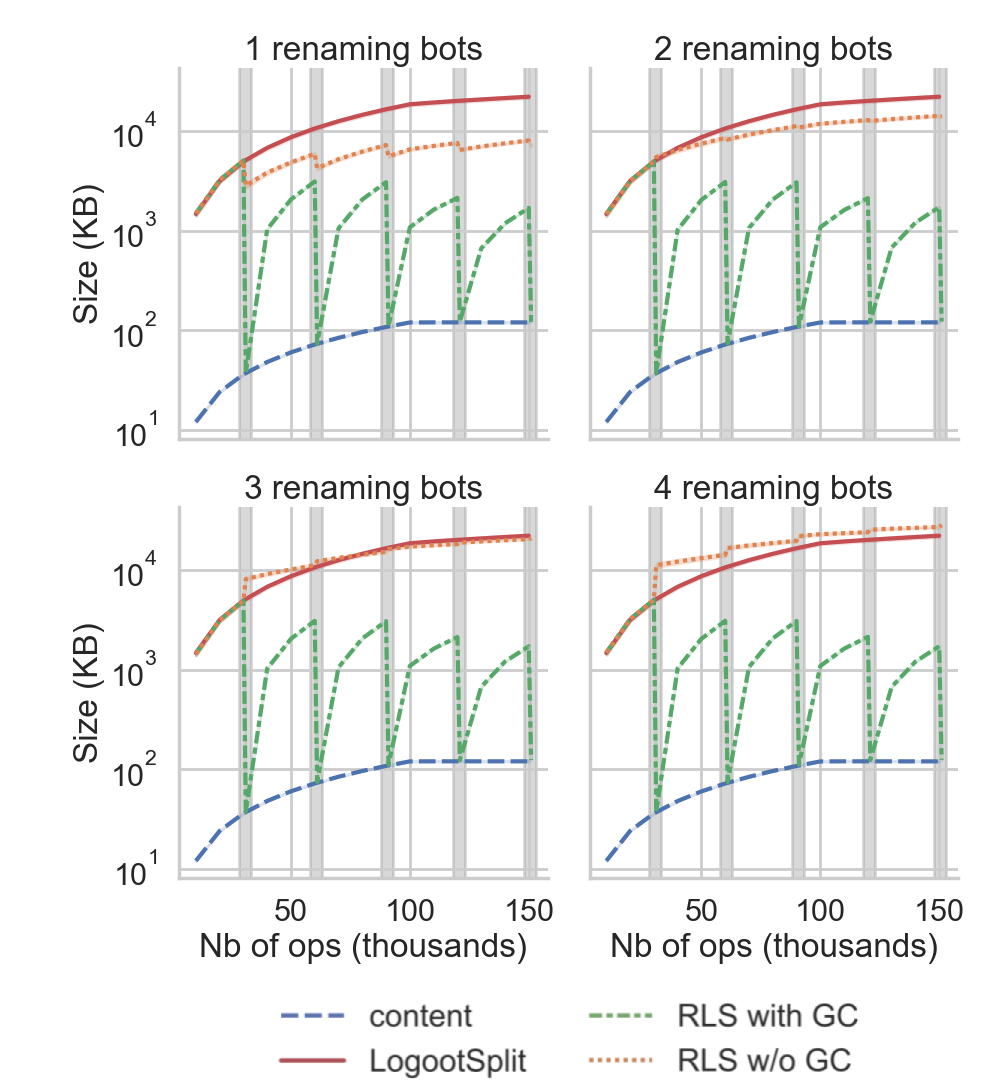
\includegraphics[width=0.7\columnwidth]{img/snapshot-sizes-alt-legende-v2.png}
  \caption{Évolution de la taille du document en fonction du \ac{CRDT} utilisé et du nombre de \emph{renaming bots} dans la collaboration}
  \label{fig:evolution-document-size}
\end{figure}

Pour chaque graphique dans la \autoref{fig:evolution-document-size}, nous représentons 4 données différentes.
La ligne tiretée bleue correspond à la taille du contenu du document, \ie du texte, tandis que la ligne continue rouge représente la taille complète du document LogootSplit.

La ligne verte pointillée-tiretée représente la taille du document RenamableLogootSplit dans son meilleur cas.
Dans ce scénario, les noeuds considèrent que les opérations \emph{rename} sont causalement stables dès qu'ils les reçoivent.
Les noeuds peuvent alors bénéficier des effets du mécanisme de renommage tout en supprimant les métadonnées qu'il introduit : les \emph{anciens états} et époques.
Ce faisant, les noeuds peuvent minimiser de manière périodique le surcoût en métadonnées de la structure de données, indépendamment du nombre de \emph{renaming bots} et d'opérations \emph{rename} concurrentes générées.

La ligne pointillée orange représente la taille du document RenamableLogootSplit dans son pire cas.
Dans ce scénario, les noeuds considèrent que les opérations \emph{rename} ne deviennent jamais causalement stables.
Les noeuds doivent alors conserver de façon permanente les métadonnées introduites par le mécanisme de renommage.
Les performances de RenamableLogootSplit diminuent donc au fur et à mesure que le nombre de \emph{renaming bots} et d'opérations \emph{rename} générées augmente.
Néanmoins, même dans ces conditions, nous observons que RenamableLogootSplit offre de meilleures performances que LogootSplit tant que le nombre de \emph{renaming bots} reste faible (1 ou 2).
Ce résultat s'explique par le fait que le mécanisme de renommage permet aux noeuds de supprimer les métadonnées de la structure de données utilisée en interne pour représenter la séquence (\ie l'arbre AVL).

Pour récapituler les résultats présentés, le mécanisme de renommage introduit un surcoût temporaire en métadonnées qui augmente avec chaque opération \emph{rename}.
Mais ce surcoût se résorbe à terme une fois que le système devient quiescent et que les opérations \emph{rename} deviennent causalement stables.
Dans la \autoref{sec:offloading-former-states}, nous détaillerons l'idée que les \emph{anciens états} peuvent être déchargés sur le disque en attendant que la stabilité causale soit atteinte pour atténuer l'impact du surcoût temporaire en métadonnées.

\subsubsection{Temps d'intégration des opérations standards}

Nous avons ensuite comparé l'évolution du temps d'intégration des opérations standards, \ie les opérations \emph{insert} et \emph{remove}, sur des documents LogootSplit et RenamableLogootSplit.
Puisque les deux types d'opérations partagent la même complexité en temps, nous avons seulement utilisé des opérations \emph{insert} dans nos benchmarks.
Nous faisons par contre la différence entre les mises à jours \emph{locales} et \emph{distantes}.
Conceptuellement, les modifications locales peuvent être décomposées comme présenté dans \cite{baquero2017pure} en les deux étapes suivantes :
\begin{enumerate*}[label=(\roman*)]
  \item la génération de l'opération correspondante
  \item l'application de l'opération correspondante sur l'état local.
\end{enumerate*}
Cependant, pour des raisons de performances, nous avons fusionné ces deux étapes dans notre implémentation.
Nous distinguons donc les résultats des modifications \emph{locales} et des modifications \emph{distantes} dans nos benchmarks.
La \autoref{fig:evolution-integration-time-insert} présente les résultats obtenus.

\begin{figure}[!ht]
  \centering
  \subfloat[Modifications locales]{
      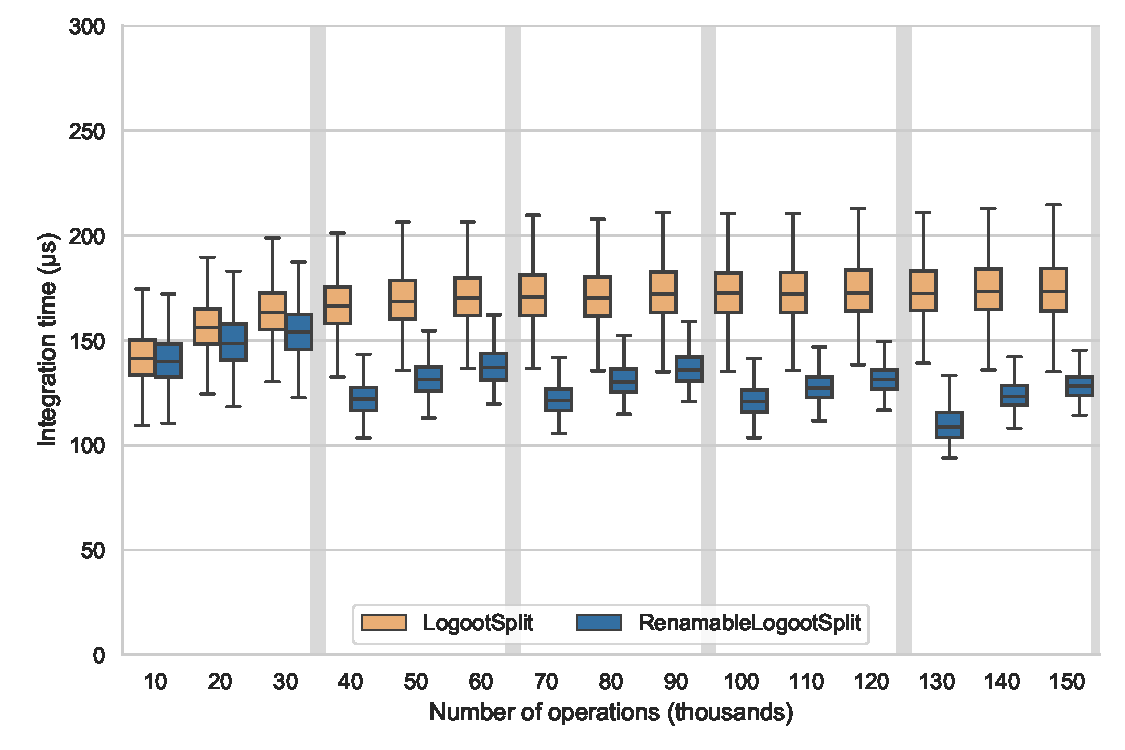
\includegraphics[width=0.45\columnwidth]{img/integration-time-boxplot-local-operations-without-outliers.pdf}
      \label{fig:evolution-integration-time-local-insert}}
  \hfil
  \subfloat[Modifications distantes]{
      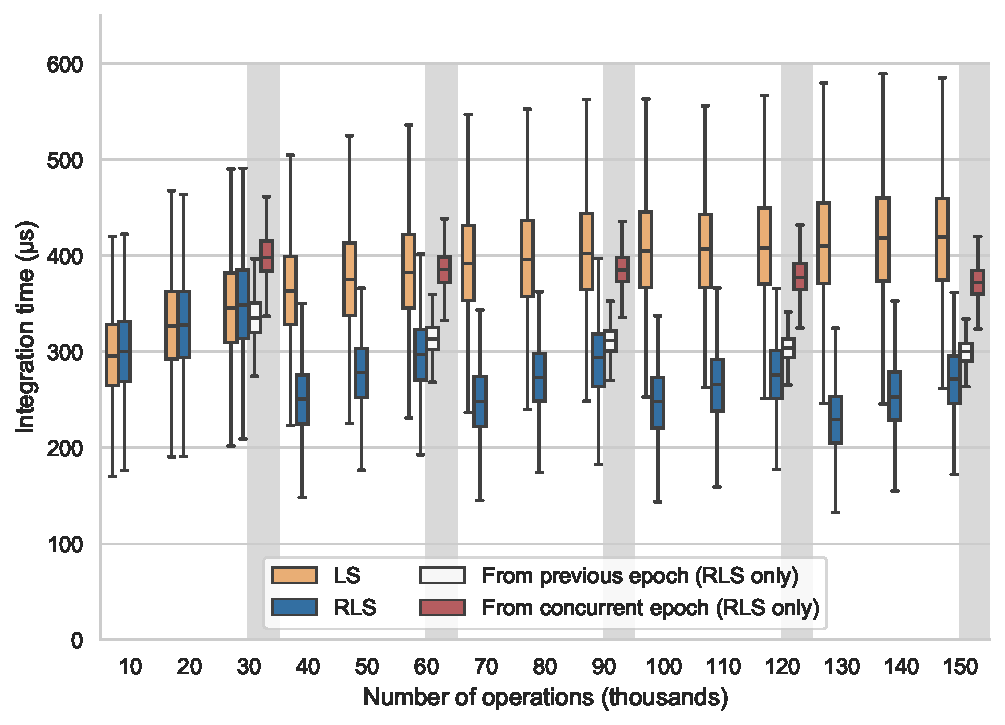
\includegraphics[width=0.45\columnwidth]{img/integration-time-boxplot-remote-operations-without-outliers.pdf}
      \label{fig:evolution-integration-time-remote-insert}}
  \caption{Temps d'intégration des opérations standards}
  \label{fig:evolution-integration-time-insert}
\end{figure}

Dans ces figures, les boxplots oranges correspondent aux temps d'intégration sur des documents LogootSplit, les boxplots bleues sur des documents RenamableLogootSplit.
Bien que les temps d'intégration soient initialement équivalents, les temps d'intégration sur des documents RenamableLogootSplit sont ensuite réduits par rapport à ceux de LogootSplit une fois que des opérations \emph{rename} ont été intégrées.
Cette amélioration s'explique par le fait que l'opération \emph{rename} optimise la représentation interne de la séquence (\ie elle réduit le nombre de blocs stockés dans l'arbre AVL).

Dans le cadre des opérations distantes, nous avons mesuré des temps d'intégration spécifiques à RenamableLogootSplit : le temps d'intégration d'opérations distantes provenant d'époques \emph{parentes} et d'époques \emph{soeurs}, respectivement affiché sous la forme de boxplots blanches et rouges dans la \autoref{fig:evolution-integration-time-remote-insert}.

Les opérations distantes provenant d'époques \emph{parentes} sont des opérations générées de manière concurrente à l'opération \emph{rename} mais appliquées après cette dernière.
Puisque l'opération doit être transformée au préalable en utilisant \textsc{renameId}, nous observons un surcoût computationnel par rapport aux autres opérations.
Mais ce surcoût est compensé par l'optimisation de la représentation interne de la séquence effectuée par l'opération \emph{rename}.

Concernant les opérations provenant d'époques \emph{soeurs}, nous observons de nouveau un surcoût puisque les noeuds doivent tout d'abord annuler les effets de l'opération \emph{rename} concurrente en utilisant \textsc{revertRenameId}.
À cause de cette étape supplémentaire, les performances de RenamableLogootSplit pour ces opérations sont comparables à celles de LogootSplit.

Pour récapituler, les fonctions de transformation ajoutent un surcoût aux temps d'intégration des opérations concurrentes aux opérations \emph{rename}.
Malgré ce surcoût, RenamableLogootSplit offre de meilleures performances que LogootSplit pour intégrer ces opérations grâce aux réductions de la taille de l'état effectuées par les opérations \emph{rename}.
Cependant, cette affirmation n'est vraie que tant que la distance entre l'époque de génération de l'opération et l'époque courante du noeud reste limitée, puisque les performances de RenamableLogootSplit dépendent linéairement de cette dernière (cf. \autoref{tab:time-complexity-operations}).
Néanmoins, ce surcoût ne concerne que les opérations concurrentes aux opérations \emph{rename}.
Il ne concerne pas la majorité des opérations, \ie les opérations générées entre deux séries d'opérations \emph{rename}.
Ces opérations, elles, ne souffrent d'aucun surcoût tout en bénéficiant des réductions de taille de l'état.

\subsubsection{Temps d'intégration de l'opération de renommage}

Finalement, nous avons mesuré l'évolution du temps d'intégration de l'opération \emph{rename} en fonction du nombre d'opérations émises précédemment, \ie en fonction de la taille de l'état.
Comme précédemment, nous distinguons les performances des modifications \emph{locales} et \emph{distantes}.

Nous rappellons que le traitement d'une opération \emph{rename} dépend de l'ordre défini par la relation \emph{priority} entre l'époque qu'elle introduit et l'époque courante du noeud qui intègre l'opération.
Le cas des opérations \emph{rename} distantes se décompose donc en trois catégories.
Les opérations \emph{distantes directes} désignent les opérations \emph{rename} distantes qui introduisent une nouvelle époque \emph{enfant} de l'époque courante du noeud.
Les opérations \emph{concurrentes introduisant une plus grande} (resp. \emph{petite}) \emph{époque} désignent les opérations \emph{rename} qui introduisent une époque \emph{soeur} de l'époque courante du noeud.
D'après la relation \emph{priority}, l'époque introduite est plus grande (resp. petite) que l'époque courante du noeud.
Les résultats obtenus sont présentés dans le \autoref{tab:evolution-integration-time-rename}.

\begin{table}[!ht]
  \centering
  \caption{Temps d'intégration de l'opération \emph{rename}}
  \label{tab:evolution-integration-time-rename}
  \resizebox{.8\columnwidth}{!}{
    \begin{tabular}{lrrrrrr}
      \toprule
      \multicolumn{2}{c}{Paramètres} & \multicolumn{5}{c}{Temps d'intégration (ms)} \\
      \cmidrule(lr){1-2} \cmidrule(lr){3-7}
      Type & Nb Ops (k) &  Moyenne & Médiane &    IQR & 1\textsuperscript{er} Percent. & 99\textsuperscript{ème} Percent. \\
      \midrule
      Locale & 30  & 41.8 &   38.7 &   5.66 &       37.3 &        71.7 \\
          & 60  & 78.3 &   78.2 &   1.58 &       76.2 &        81.4 \\
          & 90  &  119 &    119 &   2.17 &        116 &         124 \\
          & 120 &  144 &    144 &   3.24 &        139 &         149 \\
          & 150 &  158 &    158 &   3.71 &        153 &         164 \\
      \cmidrule{1-7}
      Distante directe & 30  &  481 &    477 &   15.2 &        454 &         537 \\
          & 60  &  982 &    978 &   28.9 &        926 &        1073 \\
          & 90  & 1491 &   1482 &   58.8 &       1396 &        1658 \\
          & 120 & 1670 &   1664 &     41 &       1568 &        1814 \\
          & 150 & 1694 &   1676 &   60.6 &       1591 &        1853 \\
      \cmidrule{1-7}
      Cc. int. plus grande époque & 30  &  644 &    644 &   16.6 &        620 &         683 \\
          & 60  & 1318 &   1316 &   26.5 &       1263 &        1400 \\
          & 90  & 1998 &   1994 &   46.6 &       1906 &        2112 \\
          & 120 & 2240 &   2233 &     54 &       2144 &        2368 \\
          & 150 & 2242 &   2234 &   63.5 &       2139 &        2351 \\
      \cmidrule{1-7}
      Cc. int. plus petite époque & 30  & 1.36 &    1.3 & 0.038 &       1.22 &        3.53 \\
          & 60  & 2.82 &   2.69 &  0.476 &       2.43 &        4.85 \\
          & 90  & 4.45 &   4.23 &    1.1 &       3.69 &        5.81 \\
          & 120 & 5.33 &    5.1 &   1.34 &       4.42 &        8.78 \\
          & 150 & 5.53 &   5.26 &   1.05 &       4.84 &         8.7 \\
      \bottomrule
    \end{tabular}
  }
\end{table}

Le principal résultat de ces mesures est que les opérations \emph{rename} sont particulièrement coûteuses quand comparées aux autres types d'opérations.
Les opérations \emph{rename} locales s'intègrent en centaines de millisecondes tandis que les opérations \emph{distantes directes} et \emph{concurrentes introduisant une plus grande époque} s'intègrent en secondes lorsque la taille du document dépasse 40k éléments.
Ces résultats s'expliquent facilement par la complexité en temps de l'opération \emph{rename} qui dépend supra-linéairement du nombre de blocs et d'éléments stockés dans l'état (cf. \autoref{tab:time-complexity-operations}).
Il est donc nécessaire de prendre en compte ce résultat et de
\begin{enumerate*}[label=(\roman*)]
  \item concevoir des stratégies de génération des opérations \emph{rename} pour éviter d'impacter négativement l'expérience utilisateur
  \item proposer des versions améliorées des algorithmes \textsc{renameId} et \textsc{revertRenameId} pour réduire ces temps d'intégration :
\end{enumerate*}

\begin{itemize}
  \item Au lieu d'utiliser \textsc{renameId}, qui renomme l'état identifiant par identifiant, nous pourrions définir et utiliser \textsc{renameBlock}.
    Cette fonction permettrait de renommer l'état bloc par bloc, offrant ainsi une meilleur complexité en temps.
    De plus, puisque les opérations \emph{rename} fusionnent les blocs existants en un unique bloc, \textsc{renameBlock} permettrait de mettre en place un cercle vertueux où chaque opération \emph{rename} réduirait le temps d'exécution de la suivante.
  \item Puisque chaque appel à \textsc{revertRenameId} et \textsc{revertRenameId} est indépendant des autres, ces fonctions sont adaptées à la programmation parallèle.
    Au lieu de renommer les identifiants (ou blocs) de manière séquentielle, nous pourrions diviser la séquence en plusieurs parties et les renommer en parallèle.
\end{itemize}

Un autre résultat intéressant de ces benchmarks est que les opérations \emph{concurrentes introduisant une plus petite époque} sont rapides à intégrer.
Puisque ces opérations introduisent une époque qui n'est pas sélectionnée comme nouvelle époque cible, les noeuds ne procèdent pas au renommage de leur état.
L'intégration des opérations \emph{concurrentes introduisant une plus petite époque} consiste simplement à ajouter l'époque introduite et l'\emph{ancien état} correspondant à l'\emph{arbre des époques}.
Les noeuds peuvent donc réduire de manière significative le coût d'intégration d'un ensemble d'opérations \emph{rename} concurrentes en les appliquant dans l'ordre le plus adapté en fonction du contexte.
Nous développons ce sujet dans la \autoref{sec:report-transition-to-target-epoch}.

\subsubsection{Temps pour rejouer le log d'opérations}

Afin de comparer les performances de RenamableLogootSplit et de LogootSplit de manière globale, nous avons mesuré le temps nécessaire pour un nouveau noeud pour rejouer l'entièreté du log d'opérations d'une session de collaboration, en fonction du nombre de \emph{renaming bots} de la session.
Nous présentons les résultats obtenus dans la \autoref{fig:time-to-replay-log}.

\begin{figure}[!ht]
  \centering
  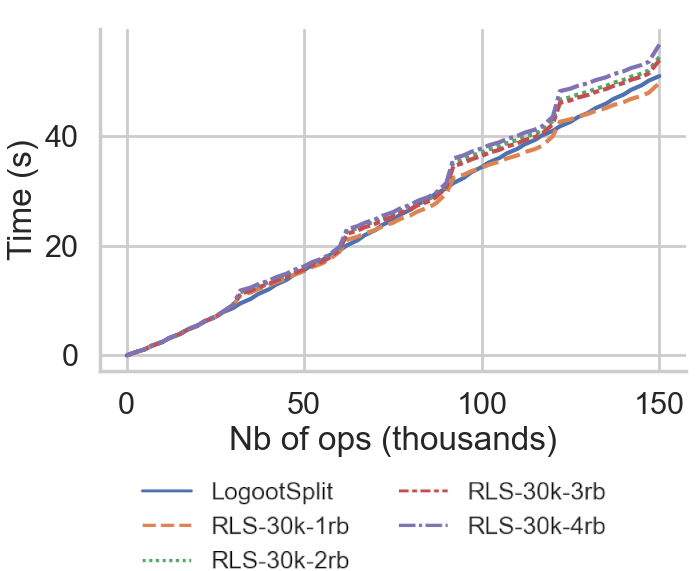
\includegraphics[width=0.7\columnwidth]{img/replay-log-30k-with-legend.png}
  \caption{Progression du nombre d'opérations du log rejouées en fonction du temps}
  \label{fig:time-to-replay-log}
\end{figure}

Nous observons que le gain sur le temps d'intégration des opérations \emph{insert} et \emph{remove} permet initialement de contrebalancer le surcoût des opérations \emph{rename}.
Mais au fur et à mesure que la collaboration progresse, le temps nécessaire pour intégrer les opérations \emph{rename} augmente car plus d'éléments sont impliqués.
Cette tendance est accentuée dans les scénarios avec des opérations \emph{rename} concurrentes.

Dans un cas réel d'utilisation, ce scénario (\ie rejouer l'entièreté du log) ne correspond pas au scénario principal et peut être mitigé, par exemple en utilisant un mécanisme de compression du log d'opérations.
Dans la \autoref{sec:rename-as-compression-mechanism}, nous présentons comment mettre en place un tel mécanisme en se basant justement sur les possibilités offertes par l'opération \emph{rename}.

\subsubsection{Impact de la fréquence de l'opération \emph{rename} sur les performances}

Pour évaluer l'impact de la fréquence de l'opération \emph{rename} sur les performances, nous avons réalisé un benchmark supplémentaire.
Ce benchmark consiste à rejouer les logs d'opérations des simulations en utilisant divers \acp{CRDT} et configurations : LogootSplit, RenamableLogootSplit effectuant des opérations \emph{rename} toutes les 30k opérations, RenamableLogootSplit effectuant des opérations \emph{rename} toutes les 7.5k opérations.
Au fur et à mesure que le benchmark rejoue le log des opérations, il mesure le temps d'intégration des opérations ainsi que leur taille.
Les résultats de ce benchmark sont présentés dans le \autoref{tab:impact-frequency}.

\begin{table}[!ht]
  \centering
  \resizebox{\linewidth}{!}{
    \begin{tabular}{llrrrrrrrrrr}
      \toprule
      \multicolumn{2}{c}{Paramètres} & \multicolumn{5}{c}{Temps d'intégration ($\trm{\mu}$s)}  & \multicolumn{5}{c}{Taille (o)} \\
      \cmidrule(lr){1-2} \cmidrule(lr){3-7} \cmidrule(lr){8-12}
      Type & CRDT & Moyenne & Médiane &  IQR & 1\textsuperscript{er} Percent. & 99\textsuperscript{ème} Percent. & Moyenne & Médiane &  IQR & 1\textsuperscript{er} Percent. & 99\textsuperscript{ème} Percent. \\
      \midrule
      insert & LS &  471 &    460 &  130 &        224 &         768 &    593 &    584 & 184 &        216 &        1136 \\
      & RLS - 30k &  397 &    323 & 66.7 &        171 &         587 &    442 &    378 &  92 &        314 &         958 \\
      & RLS - 7.5k &  393 &    265 & 54.5 &        133 &         381 &    389 &    378 &   0 &        314 &         590 \\
      remove & LS &  280 &    270 & 71.4 &        140 &         435 &    632 &    618 & 184 &        250 &        1170 \\
      & RLS - 30k &  247 &    181 &   39 &       97.9 &         308 &    434 &    412 &   0 &        320 &         900 \\
      & RLS - 7.5k &  296 &    151 & 34.8 &       74.9 &         214 &    401 &    412 &   0 &        320 &         596 \\
      \midrule
      \multicolumn{2}{c}{Paramètres} & \multicolumn{5}{c}{Temps d'intégration (ms)}  & \multicolumn{5}{c}{Taille (Ko)} \\
      \cmidrule(lr){1-2} \cmidrule(lr){3-7} \cmidrule(lr){8-12}
      Type & CRDT & Moyenne & Médiane &  IQR & 1\textsuperscript{er} Percent. & 99\textsuperscript{ème} Percent. & Moyenne & Médiane &  IQR & 1\textsuperscript{er} Percent. & 99\textsuperscript{ème} Percent. \\
      \midrule
      rename & RLS - 30k & 1022 &   1188 &  425 &        540 &        1276 &   1366 &   1258 & 514 &        635 &        3373 \\
      & RLS - 7.5k &  861 &    974 &  669 &        123 &        1445 &    273 &    302 & 132 &        159 &         542 \\
      \bottomrule
    \end{tabular}
  }
  \caption{Temps d'intégration et taille des opérations par type et par fréquence d'opérations \emph{rename}}
  \label{tab:impact-frequency}
\end{table}

Concernant les temps d'intégration, nous observons des opérations \emph{rename} plus fréquentes permettent d'améliorer les temps d'intégration des opérations \emph{insert} et \emph{remove}.
Cela confirme les résultats attendus puisque l'opération \emph{rename} réduit la taille des identifiants de la structure ainsi que le nombre de blocs composant la séquence.

Nous remarquons aussi que la fréquence n'a aucun impact significatif sur le temps d'intégration des opérations \emph{rename}.
Il s'agit là aussi d'un résultat attendu puisque la complexité en temps de l'implémentation de l'opération \emph{rename} dépend du nombre d'éléments dans la séquence, un facteur qui n'est pas impacté par les opérations \emph{rename}.

Concernant la taille des opérations, nous observons que les opérations \emph{insert} et \emph{remove} de RenamableLogootSplit sont initialement plus lourdes que les opérations correspondantes de LogootSplit, notamment car elles intègrent leur époque de génération comme donnée additionnelle.
Mais alors que la taille des opérations de LogootSplit augmentent indéfiniment, celle des opérations de RenamableLogootSplit est bornée.
La valeur de cette borne est définie par la fréquence de l'opération \emph{rename}.
Cela permet à RenamableLogootSplit d'atteindre un coût moindre par opération.

D'un autre côté, le coût des opérations \emph{rename} est bien plus important (1000x) que celui des autres types d'opérations.
Ceci s'explique par le fait que l'opération \emph{rename} intègre l'\emph{ancien état}, \ie la liste de tous les blocs composant l'état de la séquence au moment de la génération de l'opération.
Cependant, nous observons le même phénomène pour les opérations \emph{rename} que pour les autres opérations : la fréquence des opérations \emph{rename} permet d'établir une borne pour la taille des opérations \emph{rename}.
Nous pouvons donc choisir d'émettre fréquemment des opérations \emph{rename} pour limiter leur taille respective.
Ceci implique néanmoins un surcoût en computations pour chaque opération \emph{rename} dans l'implémentation actuelle.
Nous présentons une autre approche possible pour limiter la taille des opérations \emph{rename} dans la \autoref{sec:compression-rename}.
Cette approche consiste à implémenter un mécanisme de compression pour les opérations \emph{rename} pour ne transmettre que les composants nécessaires à l'identifiant de chaque bloc de l'\emph{ancien état}.

\section{Discussion}

\mnnote{TODO:
  Ajouter une partie sur la discussion qu'on a pu avoir avec les reviewers sur la présence de pierres tombales dans RenamableLogootSplit, et comment ces pierres tombales diffèrent de celles présentent dans WOOT et RGA.
}

\subsection{Stratégie de génération des opérations \emph{rename}}

Comme indiqué dans la \autoref{sec:def-rename-op}, les opérations \emph{rename} sont des opérations systèmes.
C'est donc aux concepteurs de systèmes qu'incombe la responsabilité de déterminer quand les noeuds devraient générer des opérations \emph{rename} et de définir une stratégie correspondante.
Il n'existe cependant pas de solution universelle, chaque système ayant ses particuliarités et contraintes.

Plusieurs aspects doivent être pris en compte lors de la définition de la stratégie de génération des opérations \emph{rename}.
Le premier porte sur la taille de la structure de données.
Comme illustré dans la \autoref{fig:evolution-document-size}, les métadonnées augmentent de manière progressive jusqu'à représenter 99\% de la structure de données.
En utilisant les opérations \emph{rename}, les noeuds peuvent supprimer les métadonnées et ainsi réduire la taille de la structure à un niveau acceptable.
Pour déterminer quand générer des opérations \emph{rename}, les noeuds peuvent donc monitorer le nombre d'opérations effectuées depuis la dernière opération \emph{rename}, le nombre de blocs qui composent la séquence ou encore la taille des identifiants.

Un second aspect à prendre en compte est le temps d'intégration des opérations \emph{rename}.
Comme indiqué dans le \autoref{tab:evolution-integration-time-rename}, l'intégration des opérations \emph{rename} distantes peut nécessiter des secondes si elles sont retardées trop longtemps.
Bien que les opérations \emph{rename} travaillent en coulisses, elles peuvent néanmoins impacter négativement l'expérience utilisateur.
Notamment, les noeuds ne peuvent pas intégrer d'autres opérations \emph{distantes} tant qu'ils sont en train de traiter des opérations \emph{rename}.
Du point de vue des utilisateurs, les opérations \emph{rename} peuvent alors être perçues comme des pics de latence.
Dans le domaine de l'édition collaborative temps réel, \textcite{2014-effect-delay-collaborative-editing-ignat,2015-cope-delay-collaborative-note-taking-ignat} ont montré que le délai dégradait la qualité des collaborations.
Il est donc important de générer fréquemment des opérations \emph{rename} pour conserver leur temps d'intégration sous une limite perceptible.

Finalement, le dernier aspect à considérer est le nombre d'opérations \emph{rename} concurrentes.
La \autoref{fig:evolution-document-size} montre que les opérations \emph{rename} concurrentes accroissent la taille de la structure de données tandis que la \autoref{fig:time-to-replay-log} illustre qu'elles augmentent le temps nécessaire pour rejouer le log d'opérations.
La stratégie proposée doit donc viser à minimiser le nombre d'opérations \emph{rename} concurrentes générées.
Cependant, elle doit éviter d'utiliser des coordinations synchrones entre les noeuds pour cela (\eg algorithmes de consensus), pour des raisons de performances.
Pour réduire la probabilité de générer des opérations \emph{rename} concurrentes, plusieurs méthodes peuvent être proposées.
Par exemple, les noeuds peuvent monitorer à quels autres noeuds ils sont connectés actuellement et déléguer au noeud ayant le plus grand \emph{identifiant de noeud} la responsabilité de générer les opérations \emph{rename}.

Pour récapituler, nous pouvons proposer plusieurs stragégies de génération des opérations \emph{rename}, pour minimiser de manière individuelle chacun des paramètres présentés.
Mais bien que certaines de ces stratégies convergent (minimiser la taille de la structure de données et minimiser le temps d'intégration des opérations \emph{rename}), d'autres entrent en conflit (générer une opération \emph{rename} dès qu'un seuil est atteint vs. minimiser le nombre d'opérations \emph{rename} concurrentes générées).
Les concepteurs de systèmes doivent proposer un compromis entre les différents paramètres en fonction des contraintes du système concerné (application temps réel ou asynchrone, limitations matérielles des noeuds...).
Il est donc nécessaire d'analyser le système pour évaluer ses performances sur chaque aspect, ses usages et trouver le bon compromis entre tous les paramètres de la stratégie de renommage.
Par exemple, dans le contexte des systèmes d'édition collaborative temps réel, \cite{2014-effect-delay-collaborative-editing-ignat} a montré que le délai diminue la qualité de la collaboration.
Dans de tels systèmes, nous viserions donc à conserver le temps d'intégration des opérations (en incluant les opérations \emph{rename}) en dessous du temps limite correspondant à leur perception par les utilisateurs.

\subsection{Stockage des états précédents sur disque}

\label{sec:offloading-former-states}

Les noeuds doivent conserver les \emph{anciens états} associés aux opérations \emph{rename} pour transformer les opérations issues d'époques précédentes ou concurrentes.
Les noeuds peuvent recevoir de telles opérations dans deux cas précis :
\begin{enumerate*}[label=(\roman*)]
  \item des noeuds ont émis récemment des opérations \emph{rename}
  \item des noeuds se sont récemment reconnectés.
\end{enumerate*}
Entre deux de ces évènements spécifiques, les \emph{anciens états} ne sont pas nécessaires pour traiter les opérations.

Nous pouvons donc proposer l'optimisation suivante : décharger les \emph{anciens états} sur le disque jusqu'à leur prochaine utilisation ou jusqu'à ce qu'ils puissent être supprimés de manière sûre.
Décharger les \emph{anciens états} sur le disque permet de mitiger le surcoût en mémoire introduit par le mécanisme de renommage.
En échange, cela augmente le temps d'intégration des opérations nécessitant un \emph{ancien état} qui a été déchargé précédemment.

Les noeuds peuvent adopter différentes stratégies, en fonction de leurs contraintes, pour déterminer les \emph{anciens états} comme déchargeables et pour les récupérer de manière préemptive.
La conception de ces stratégies peut reposer sur différentes heuristiques : les époques des noeuds actuellement connectés, le nombre de noeuds pouvant toujours émettre des opérations concurrentes, le temps écoulé depuis la dernière utilisation de l'\emph{ancien état}...

\subsection{Compression et limitation de la taille de l'opération \emph{rename}}

\label{sec:compression-rename}

Pour limiter la consommation en bande passante des opérations \emph{rename}, nous proposons la technique de compression suivante.
Au lieu de diffuser les identifiants complets formant l'\emph{ancien état}, les noeuds peuvent diffuser seulement les éléments nécessaires pour identifier de manière unique les intervalles d'identifiants.
En effet, un identifiant peut être caractérisé de manière unique par le triplet composé de l'\emph{identifiant de noeud}, du \emph{numéro de séquence} et de l'\emph{offset} de son dernier tuple.
Par conséquent, un intervalle d'identifiants peut être identifié de manière unique à partir du triplet signature de son identifiant de début et de sa longueur, \ie du quadruplet $\langle\trm{nodeId}, \trm{nodeSeq}, \trm{offsetBegin}, \trm{offsetEnd}\rangle$.
Cette méthode nous permet de réduire les données à diffuser dans le cadre de l'opération \emph{rename} à un montant fixe par intervalle.

Pour décompresser l'opération reçue, les noeuds doivent reformer les intervalles d'identifiants correspondant aux quadruplets reçus.
Pour cela, ils parcourent leur état.
Lorsqu'ils rencontrent un identifiant partageant le même couple $\langle\trm{nodeId}, \trm{nodeSeq}\rangle$ qu'un des intervalles de l'opération \emph{rename}, les noeuds disposent de l'ensemble des informations requises pour le reconstruire.
Cependant, certains couples $\langle\trm{nodeId}, \trm{nodeSeq}\rangle$ peuvent avoir été supprimés en concurrence et ne plus être présents dans la séquence.
Dans ce cas, il est nécessaire de parcourir le log des opérations \emph{remove} concurrentes pour retrouver les identifiants correspondants et reconstruire l'opération \emph{rename} originale.

Grâce à cette méthode de compression, nous pouvons instaurer une taille maximale à l'opération \emph{rename}.
En effet, les noeuds peuvent émettre une opération \emph{rename} dès que leur état courant atteint un nombre donné d'intervalles d'identifiants, bornant ainsi la taille du message à diffuser.

\subsection{Définition de relations de priorité pour minimiser les traitements}

\label{sec:alt-priority-relation}

Bien que la relation \emph{priority} proposée dans la \autoref{sec:priority} est simple et garantit que tous les noeuds désignent la même époque comme époque cible, elle introduit un surcoût computationnel significatif dans certains cas.
La \autoref{fig:worst-case-priority} présente un tel cas.

\begin{figure}[!ht]
  \subfloat[Exécution d'opérations \emph{rename} concurrentes]{
      \begin{minipage}{\linewidth}
          \centering
          \resizebox{.7\linewidth}{!}{
            \begin{tikzpicture}
              \path
                node {\textbf{A}}
                ++(0:0.5) node (a0) {}
                ++(0:1) node[point, label=above:{rename to \epoch{A1}}] (a1) {}
                ++(0:2) node (a-receives-b7) {}
                ++(0:1) node [point, label=above:{rename to \epoch{A10}}] (a10) {}
                ++(0:1) node (a11) {}
                ++(0:1) node (a99) {}
                ++(0:1) node[point, label=above:{rename to \epoch{A100}}] (a100) {}
                ++(0:1.5) node (a-receives-c1) {}
                ++(0:1.5) node (a-end) {};

              \draw[thick] (a0) --  (a1) -- (a10) -- (a11);
              \draw[dotted] (a11) -- (a99);
              \draw[->, thick] (a99) -- (a100) -- (a-end);

              \path
                  ++(270:2) node {\textbf{B}}
                  ++(0:0.5) node (b0) {}
                  ++(0:2) node (b-receives-a1) {}
                  ++(0:0.5) node[point, label=below:{rename to \epoch{B2}}] (b7) {}
                  ++(0:2.5) node (b8) {}
                  ++(0:1) node (b99) {}
                  ++(0:2.5) node (b-receives-a100) {}
                  ++(0:1.5) node (b-end) {};

              \draw[thick] (b0) -- (b7) -- (b8);
              \draw[dotted] (b8) -- (b99);
              \draw[->, thick] (b99) -- (b-end);

              \path
                  ++(270:4) node {\textbf{C}}
                  ++(0:0.5) node (c0) {}
                  ++(0:2) node[point, label=below:{rename to \epoch{C1}}] (c1) {}
                  ++(0:3) node (c2) {}
                  ++(0:1) node (c99) {}
                  ++(0:4) node (c-end) {};

                \draw[thick] (c0) -- (c1) -- (c2);
                \draw[dotted] (c2) -- (c99);
                \draw[->, thick] (c99) -- (c-end);

              \draw[->, dashed, shorten >= 1] (a1) -- (b-receives-a1);
              \draw[->, dashed, shorten >= 1] (b7) -- (a-receives-b7);
              % \draw[->, dashed, shorten >= 1] (a100) -- (b-receives-a100);
              \draw[->, dashed, shorten >= 1] (c1) -- (a-receives-c1);
            \end{tikzpicture}
          }
          \label{fig:worst-case-priority-execution}
      \end{minipage}}
  \hfil
  \subfloat[\emph{Arbre des époques} final correspondant avec la relation \emph{priority} illustrée]{
      \begin{minipage}{\linewidth}
          \centering
          \resizebox{.15\linewidth}{!}{
            \begin{tikzpicture}
                \path
                    node[op] (e0) {\epoch{0}}
                    ++(225:1.5) node[op] (eA1) {\epoch{A1}}
                    ++(270:1.5) node[op] (eB7) {\epoch{B7}}
                    ++(270:1.5) node[op] (eA10) {\epoch{A10}}
                    ++(270:1) node (eA11) {}
                    ++(270:0.5) node (eA99) {}
                    ++(270:1) node[op] (eA100) {\epoch{A100}};
                \path
                    ++(315:1.5) node[op, red] (eC1) {\epoch{C1}};

                \draw[->, thick] (e0) edge (eA1) (eA1) edge (eB7) (eB7) edge (eA10) (eA10) edge (eA11) (eA99) edge(eA100) (e0) edge (eC1);
                \draw[dotted] (eA11) edge (eA99);
                \draw[->, dashed, thick, red] (eC1.270) -- (eA100.45) (eA100.50) -- (eA10.315) (eA10.45) -- (eB7.315) (eB7.45) -- (eA1.315) (eA1.0) -- (e0.270);
            \end{tikzpicture}
          }
          \label{fig:worst-case-priority-tree}
      \end{minipage}}
  \caption{Livraison d'une opération \emph{rename} d'un noeud }
  \label{fig:worst-case-priority}
\end{figure}

Dans cet exemple, les noeuds A et B éditent en collaboration un document.
Au fur et à mesure de leur collaboration, ils effectuent plusieurs opérations \emph{rename}.
Cependant, après un nombre conséquent de modifications de leur part, un autre noeud C se reconnecte.
Celui-ci leur transmet sa propre opération \emph{rename}, concurrente à toutes leurs opérations.
D'après la relation \emph{priority}, nous avons \epoch{0}~\lepoch~\epoch{A1}~\lepoch~...~\lepoch~\epoch{A100}~\lepoch~\epoch{C1}.
La nouvelle époque cible étant \epoch{C1}, les noeuds A et B doivent pour l'atteindre annuler successivement l'ensemble des opérations \emph{rename} composant leur branche de l'\emph{arbre des époques}.
Ainsi, un noeud isolé peut forcer l'ensemble des noeuds à effectuer un lourd calcul.
Il serait plus efficace que, dans cette situation, ce soit seulement le noeud isolé qui doive se mettre à jour.

La relation \emph{priority} devrait donc être conçue pour garantir la convergence des noeuds, mais aussi pour minimiser les calculs effectués globalement par les noeuds du système.
Pour concevoir une relation \emph{priority} efficace, nous pourrions incorporer dans les opérations \emph{rename} des métriques qui représentent l'état du système et le travail accumulé sur le document (nombre de noeuds actuellement à l'époque \emph{parente}, nombre d'opérations générées depuis l'époque parente, taille du document...).
De cette manière, nous pourrions favoriser la branche de l'\emph{arbre des époques} regroupant les collaborateurs les plus actifs et empêcher les noeuds isolés d'imposer leurs opérations \emph{rename}.

Afin d'offrir une plus grande flexibilité dans la conception de la relation \emph{priority}, il est nécessaire de retirer la contrainte interdisant aux noeuds de rejouer une opération \emph{rename}.
Pour cela, un couple de fonctions réciproques doit être proposée pour \textsc{renameId} et \textsc{revertRenameId}.
Une solution alternative est de proposer une implémentation du mécanisme de renommage qui repose sur les identifiants originaux plutôt que sur ceux transformés, par exemple en utilisant le log des opérations.

\subsection{Report de la transition vers la nouvelle époque cible}

\label{sec:report-transition-to-target-epoch}

Comme illustré par le \autoref{tab:evolution-integration-time-rename}, intégrer des opérations \emph{rename} distantes est généralement coûteux.
Ce traitement peut générer un surcoût computationnel significatif en cas de multiples opérations \emph{rename} concurrentes.
En particulier, un noeud peut recevoir et intégrer les opérations \emph{rename} concurrentes dans l'ordre inverse défini par la relation \emph{priority} sur leur époques.
Dans ce scénario, le noeud considérerait chaque nouvelle époque introduite comme la nouvelle époque cible et renommerait son état en conséquence à chaque fois.

% \mnnote{TODO: Ajouter figure où noeud reçoit successivement plusieurs opérations \emph{rename} concurrentes et procéde au renommage de son état à chaque fois}

En cas d'un grand nombre d'opérations \emph{rename} concurrentes, nous proposons que les noeuds délaient le renommage de leur état vers l'époque cible jusqu'à ce qu'ils aient obtenu un niveau de confiance donné en l'époque cible.
Ce délai réduit la probabilité que les noeuds effectuent des traitements inutiles.
Plusieurs stratégies peuvent être proposées pour calculer le niveau de confiance en l'époque cible.
Ces stratégies peuvent reposer sur une variété de métriques pour produire le niveau de confiance, tel que le temps écoulé depuis que le noeud a reçu une opération \emph{rename} concurrente et le nombre de noeuds en ligne qui n'ont pas encore reçu l'opération \emph{rename}.

Durant cette période d'incertitude introduite par le report, les noeuds peuvent recevoir des opérations provenant d'époques différentes, notamment de l'époque cible.
Néanmoins, les noeuds peuvent toujours intégrer les opérations \emph{insert} et \emph{remove} en utilisant \textsc{renameId} et \textsc{revertRenameId} au prix d'un surcoût computationnel pour chaque identifiant.
Cependant, ce coût est négligeable (plusieurs centaines de microsecondes par identifiant d'après la \autoref{fig:evolution-integration-time-remote-insert}) comparé au coût de renommer, de manière inutile, complètement l'état (plusieurs centaines de milliseconds à des secondes complètes d'après le \autoref{tab:evolution-integration-time-rename}).

Notons que ce mécanisme nécessite que \textsc{renameId} et \textsc{revertRenameId} soient des fonctions réciproques.
En effet, au cours de la période d'incertitude, un noeud peut avoir à utiliser \textsc{revertRenameId} pour intégrer les identifiants d'opérations \emph{insert} distantes provenant de l'époque cible.
Ensuite, le noeud peut devoir renommer son état vers l'époque cible une fois que celle-ci a obtenu le niveau de confiance requis.
Il s'ensuit que \textsc{renameId} doit restaurer les identifiants précédemment transformés par \textsc{revertRenameId} à leur valeur initiale pour garantir la convergence.

\subsection{Utilisation de l'opération de renommage comme mécanisme de compression du log d'opérations}

\label{sec:rename-as-compression-mechanism}

Lorsqu'un nouveau pair rejoint la collaboration, il doit tout d'abord récupérer l'état courant du document avant de pouvoir participer.
Le nouveau pair utilise un mécanisme d'anti-entropie \cite{1983-anti-entropy-vv} pour récupérer l'ensemble des opérations via un autre pair.
Puis il reconstruit l'état courant en appliquant successivement chacune des opérations.
Ce processus peut néanmoins s'avérer coûteux pour les documents comprenant des milliers d'opérations.

Pour pallier ce problème, des mécanismes de compression du log ont été proposés dans la littérature.
Les approches présentées dans \cite{2002-log-compression-op-based-vcs-shen-sun, 2006-these-claudia} consistent à remplacer un sous-ensemble des opérations du log par une opération équivalente, par exemple en aggrégeant les opérations \emph{insert} adjacentes.
Une autre approche, présentée dans \cite{2014-making-op-based-crdts-op-based}, définie une relation \emph{obsolete} sur les opérations.
La relation \emph{obsolete} permet de spécifier qu'une nouvelle opération rend obsolètes des opérations précédentes et permet de les retirer du log.
Pour donner un exemple, une opération d'ajout d'un élément donné dans un OR-Set \ac{CRDT} rend obsolètes toutes les opérations précédentes d'ajout et de suppression de cet élément.

Dans notre contexte, il est intéressant de noter que l'opération \emph{rename} peut endosser un rôle comparable à ces mécanismes de compression du log.
En effet, l'opération \emph{rename} prend un état donné, somme des opérations passées, et génère en retour un nouvel état équivalent et compacté.
Une opération \emph{rename} rend donc obsolète l'ensemble des opérations dont elle dépend causalement, et peut être utilisée pour les remplacer.
En partant de cette observation, nous proposons le mécanisme de compression du log suivant.

Le mécanisme consiste à réduire le nombre d'opérations transmises à un nouveau pair rejoignant la collaboration grâce à l'opération \emph{rename} de l'époque courante.
L'opération \emph{rename} ayant introduite l'époque courante fournit un état initial au nouveau pair.
À partir de cet état initial, le nouveau pair peut obtenir l'état courant en intégrant les opérations \emph{insert} et \emph{remove} qui ont été générées de manière concurrente ou causale par rapport à l'opération \emph{rename}.
En réponse à une demande de synchronisation d'un nouveau pair, un pair peut donc simplement lui envoyer un sous-ensemble de son log composé de :
\begin{enumerate*}[label=(\roman*)]
  \item l'opération \emph{rename} ayant introduite son époque courante
  \item les opérations \emph{insert} et \emph{remove} dont l'opération \emph{rename} courante ne dépend pas causalement.
\end{enumerate*}

Notons que les données contenues dans l'opération \emph{rename} telle que nous l'avons définie précédemment (cf. \autoref{def:rename-op}) sont insuffisantes pour cette utilisation.
En effet, les données incluses (\emph{ancien état} au moment du renommage, identifiant du noeud auteur de l'opération \emph{rename} et son numéro de séquence au moment de la génération) nous permettent seulement de recréer la structure de la séquence après le renommage.
Mais le contenu de la séquence est omis, celui-ci n'étant jusqu'ici d'aucune utilité pour l'opération \emph{rename}.
Afin de pouvoir utiliser l'opération \emph{rename} comme état initial, il est nécessaire d'y inclure cette information.

De plus, des informations de causalité doivent être intégrées à l'opération \emph{rename}.
Ces informations doivent permettre aux noeuds d'identifier les opérations supplémentaires nécessaires pour obtenir l'état courant, \ie toutes les opérations desquelles l'opération \emph{rename} ne dépend pas causalement.
L'ajout à l'opération \emph{rename} d'un \emph{vecteur de version}, structure représentant l'ensemble des opérations observées par l'auteur de l'opération \emph{rename} au moment de sa génération, permettrait cela.

Nous définissons donc de la manière suivante l'opération \emph{rename} enrichie compatible avec ce mécanisme de compression du log :

\begin{definition}[rename enrichie]
  \label{def:-rich-rename-op}
  Une opération \emph{rename enrichie} est un quintuplet $\langle$nodeId, nodeSeq, formerState, versionVector, content$\rangle$ où
  \begin{itemize}
    \item nodeId est l'identifiant du noeud qui a générée l'opération \emph{rename}.
    \item nodeSeq est le numéro de séquence du noeud au moment de la génération de l'opération \emph{rename}.
    \item formerState est l'ancien état du noeud au moment du renommage.
    \item versionVector est le vecteur de version représentant l'ancien état du noeud au moment du renommage.
    \item content est le contenu du document au moment du renommage.
  \end{itemize}
\end{definition}

Ce mécanisme de compression du log introduit néanmoins le problème suivant.
Un nouveau pair synchronisé de cette manière ne possède qu'un sous-ensemble du log des opérations.
Si ce pair reçoit ensuite une demande de synchronisation d'un second pair, il est possible qu'il ne puisse répondre à la requête.
Par exemple, le pair ne peut pas fournir des opérations faisant partie des dépendances causales de l'opération \emph{rename} qui lui a servi d'état initial.

Une solution possible dans ce cas de figure est de rediriger le second pair vers un troisième pour qu'il se synchronise avec lui.
Cependant, cette solution pose des problèmes de latence/temps de réponse si le troisième pair s'avère indisponible à ce moment.
Une autre approche possible est de généraliser le processus de synchronisation que nous avons présenté ici (opération \emph{rename} comme état initial puis application des autres opérations) à l'ensemble des pairs, et non plus seulement aux nouveaux pairs.
Nous présentons les avantages et inconvénients de cette approche dans la sous-section suivante.

% \mnnote{TODO: Étudier si y a un intérêt à privilégier la synchronisation basée sur l'intégration successive de toutes les opérations quand on a cette méthode de synchronisation par snapshot/checkpoint de possible}

\subsection{Implémentation alternative de l'intégration de l'opération \emph{rename} basée sur le log d'opérations}

Nous avons décrit précédemment dans la \autoref{sec:integration-process-rename-op}, et plus précisément dans l'\autoref{alg:renameRemote}, le processus d'intégration de l'opération \emph{rename} évaluée dans ce manuscrit.
Pour rappel, le processus consiste à
\begin{enumerate*}[label=(\roman*)]
  \item identifier le chemin entre l'époque courante et l'époque cible
  \item appliquer les fonctions de transformations \textsc{revertRenameId} et \textsc{renameId} à l'ensemble des identifiants composant l'état courant
  \item re-créer une séquence à partir des nouveaux identifiants calculés et du contenu courant.
\end{enumerate*}

Dans cette section, nous abordons une implémentation alternative de l'intégration de l'opération \emph{rename}.
Cette implémentation repose sur le log des opérations.

Cette implémentation se base sur les observations suivantes :
\begin{enumerate*}[label=(\roman*)]
  \item L'état courant est obtenu en intégrant successivement l'ensemble des opérations.
  \item L'opération \emph{rename} est une opération subsumant les opérations passées : elle prend un état donné (l'\emph{ancien état}), somme des opérations précédentes, et génère un nouvel état équivalent compacté.
  \item L'ordre d'intégration des opérations concurrentes n'a pas d'importance sur l'état final obtenu.
\end{enumerate*}

Ainsi, pour intégrer une opération \emph{rename} distante, un noeud peut
\begin{enumerate*}[label=(\roman*)]
  \item générer l'état correspondant au renommage de l'\emph{ancien état}
  \item identifier le chemin entre l'époque courante et l'époque cible
  \item identifier les opérations concurrentes à l'opération \emph{rename} présentes dans son log
  \item transformer et intégrer successivement les opérations concurrentes à l'opération \emph{rename} à ce nouvel état
\end{enumerate*}

Cet algorithme est équivalent à ré-ordonner le log des opérations de façon à intégrer les opérations précédant l'opération \emph{rename}, puis à intégrer l'opération \emph{rename} elle-même, puis à intégrer les opérations concurrentes à cette dernière.

Cette approche présente plusieurs avantages par rapport à l'implémentation décrite dans la \autoref{sec:integration-process-rename-op}.
Tout d'abord, elle modifie le facteur du nombre de transformations à effectuer.
La version décrite dans la \autoref{sec:integration-process-rename-op} transforme de l'époque courante vers l'époque cible chaque identifiant (ou chaque bloc si on dispose de \textsc{renameBlock}) de l'état courant.
La version présentée ici effectue une transformation pour chaque opération du log concurrente à l'opération \emph{rename} à intégrer.
Le nombre de transformation peut donc être réduit de plusieurs ordres de grandeur avec cette approche, notamment si les opérations sont propagées aux pairs du réseau rapidement.

Un autre avantage de cette approche est qu'elle permet de récupérer et de réutiliser les identifiants originaux des opérations.
Lorsqu'une suite de transformations est appliquée sur les identifiants d'une opération, elle est appliquée sur les identifiants originaux et non plus sur leur équivalents présents dans l'état courant.
Ceci permet de réinitialiser les transformations appliquées à un identifiant et d'éviter le cas de figure mentionné dans la \autoref{sec:reverting-rename-ops} : le cas où \textsc{revertRenameId} est utilisé pour retirer l'effet d'une opération \emph{rename} sur un identifiant, avant d'utiliser \textsc{renameId} pour ré-intégrer l'effet de la même opération \emph{rename}.
Cette implémentation supprime donc la contrainte de définir un couple de fonctions réciproques \textsc{renameId} et \textsc{revertRenameId}, ce qui nous offre une plus grande flexibilité dans le choix de la relation \lepoch et du couple de fonctions \textsc{renameId} et \textsc{revertRenameId}.

Cette implémentation dispose néanmoins de plusieurs limites.
Tout d'abord, elle nécessite que chaque noeud maintienne localement le log des opérations.
Les métadonnées accumulées par la structure de données répliquées vont alors croître avec le nombre d'opérations effectuées.
Cependant, ce défaut est à nuancer.
En effet, les noeuds doivent déjà maintenir le log des opérations pour le mécanisme d'anti-entropie, afin de renvoyer une opération passée à un noeud l'ayant manquée.
Plus globalement, les noeuds doivent aussi conserver le log des opérations pour permettre à un nouveau noeud de rejoindre la collaboration et de calculer l'état courant en rejouant l'ensemble des opérations.
Il s'agit donc d'une contrainte déjà imposée aux noeuds pour d'autres fonctionnalités du système.

Un autre défaut de cette implémentation est qu'elle nécessite de détecter les opérations concurrentes à l'opération \emph{rename} à intégrer.
Cela implique d'ajouter des informations de causalité à l'opération \emph{rename}, tel qu'un vecteur de version.
Cependant, la taille des vecteurs de version croît de façon monotone avec le nombre de noeuds qui participent à la collaboration.
Diffuser cette information à l'ensemble des noeuds peut donc représenter un coût significatif dans les collaborations à large échelle.
Néanmoins, il faut rappeler que les noeuds échangent déjà régulièrement des vecteurs de version dans le cadre du fonctionnement du mécanisme d'anti-entropie.
Les opérations \emph{rename} étant rares en comparaison, ce surcoût nous paraît acceptable.

Finalement, cette approche implique aussi de parcourir le log des opérations à la recherche d'opérations concurrentes.
Comme dit précédemment, la taille du log croît de façon monotone au fur et à mesure que les noeuds émettent des opérations.
Cette étape du nouvel algorithme d'intégration de l'opération \emph{rename} devient donc de plus en plus coûteuse.
Des méthodes permettent néanmoins de réduire son coût computationnel.
Notamment, chaque noeud traquent les informations de progression des autres noeuds afin de supprimer les métadonnées du mécanisme de renommage (cf. \autoref{sec:gc-mechanism}).
Ces informations permettent de déterminer la stabilité causale des opérations et donc d'identifier les opérations qui ne peuvent plus être concurrentes à une nouvelle opération \emph{rename}.
Les noeuds peuvent ainsi maintenir, en plus du log complet des opérations, un log composé uniquement des opérations non stables causalement.
Lors du traitement d'une nouvelle opération \emph{rename}, les noeuds peuvent alors parcourir ce log réduit à la recherche des opérations concurrentes.

% \mnnote{TODO: Ajouter conclusion à cette sous-section}

\section{Comparaison avec les approches existantes}

\subsection{Core-Nebula}

L'approche \emph{core-nebula}\cite{letia:hal-01248270,zawirski:hal-01248197} a été proposée pour réduire la taille des identifiants dans Treedoc \cite{5158449}.
Dans ces travaux, les auteurs définissent l'opération \emph{rebalance} qui permet aux noeuds de réassigner des identifiants plus courts aux éléments du document.
Cependant, cette opération \emph{rebalance} n'est ni commutative avec les opérations \emph{insert} et \emph{remove}, ni avec elle-même.
Pour assurer la convergence à terme \cite{10.1145/224057.224070}, l'approche \emph{core-nebula} empêche la génération d'opérations \emph{rebalance} concurrentes.
Pour ce faire, l'approche requiert un consensus entre les noeuds pour générer les opérations \emph{rebalance}.
Des opérations \emph{insert} et \emph{remove} sont elles toujours générées sans coordination entre les noeuds et peuvent donc être concurrentes aux opérations \emph{rebalance}.
Pour gérer les opérations concurrentes aux opérations \emph{rebalance}, les auteurs proposent de transformer les opérations concernées par rapport aux effets des opérations \emph{rebalance}, à l'aide un mécanisme de \emph{catch-up}, avant de les appliquer.

Cependant, les protocoles de consensus ne passent pas à l'échelle et ne sont pas adaptés aux systèmes distribués à large échelle.
Pour pallier ce problème, l'approche \emph{core-nebula} propose de répartir les noeuds dans deux groupes : le \emph{core} et la \emph{nebula}.
Le \emph{core} est un ensemble, de taille réduite, de noeuds stables et hautement connectés tandis que la \emph{nebula} est un ensemble, de taille non-bornée, de noeuds.
Seuls les noeuds du \emph{core} participent à l'exécution du protocole de consensus.
Les noeuds de la \emph{nebula} contribuent toujours au document par le biais des opérations \emph{insert} et \emph{remove}.

Notre travail peut être vu comme une extension de celui présenté dans \emph{core-nebula}.
Avec RenamableLogootSplit, nous adaptons l'opération \emph{rebalance} et le mécanisme de \emph{catch-up} à LogootSplit pour tirer partie de la fonctionnalité offerte par les blocs.
De plus, nous proposons un mécanisme pour supporter les opérations \emph{rename} concurrentes, ce qui supprime la nécessité de l'utilisation d'un protocole de consensus.
Notre contribution est donc une approche plus générique puisque RenamableLogootSplit est utilisable dans des systèmes composés d'un \emph{core} et d'une \emph{nebula}, ainsi que dans les systèmes ne disposant pas de noeuds stables pour former un \emph{core}.

Dans les systèmes disposant d'un \emph{core}, nous pouvons donc combiner RenamableLogootSplit avec un protocole de consensus pour éviter la génération d'opérations \emph{rename} concurrentes.
Cette approche offre plusieurs avantages.
Elle permet de se passer de tout ce qui à attrait au support d'opérations \emph{rename} concurrentes, \ie la définition d'une relation \emph{priority} et l'implémentation de \textsc{revertRenameId}.
Elle permet aussi de simplifier l'implémentation du mécanisme de récupération de mémoire des époques et \emph{anciens états} pour reposer seulement sur la stabilité causale des opérations.
Concernant ses performances, cette approche se comporte de manière similaire à RenamableLogootSplit avec un seul \emph{renaming bot} (cf. \autoref{sec:evaluation-results}), mais avec un surcoût correspondant au coût du protocole de consensus sélectionné.

\subsection{LSEQ}

L'approche LSEQ \cite{lseq2013, lseq2017} est une approche visant à réduire la croissance des identifiants dans les Séquences \acp{CRDT} à identifiants densément ordonnés.
Au lieu de réduire périodiquement la taille des métadonnées liées aux identifiants à l'aide d'un mécanisme de renommage coûteux, les auteurs définissent de nouvelles stratégies d'allocation des identifiants pour réduire leur vitesse de croissance.
Dans ces travaux, les auteurs notent que la stratégie d'allocation des identifiants proposée dans Logoot \cite{WeissICDCS09} n'est adaptée qu'à un seul comportement d'édition : de gauche à droite, de haut en bas.
Si les insertions sont effectuées en suivant d'autres comportements, les identifiants générés saturent rapidement l'espace des identifiants pour une taille donnée.
Les insertions suivantes déclenchent alors une augmentation de la taille des identifiants.
En conséquent, la taille des identifiants dans Logoot augmente de façon linéaire au nombre d'insertions, au lieu de suivre la progression logarithmique attendue.

LSEQ définit donc plusieurs stratégies d'allocation d'identifiants adaptées à différents comportements d'édition.
Les noeuds choisissent aléatoirement une de ces stratégies pour chaque taille d'identifiants.
De plus, LSEQ adopte une structure d'arbre exponentiel pour allouer les identifiants : l'intervalle des identifiants possibles double à chaque fois que la taille des identifiants augmente.
Cela permet à LSEQ de choisir avec soin la taille des identifiants et la stratégie d'allocation en fonction des besoins.
En combinant les différentes stratégies d'allocation avec la structure d'arbre exponentiel, LSEQ offre une croissance polylogarithmique de la taille des identifiants en fonction du nombre d'insertions.

Bien que l'approche LSEQ réduit la vitesse de croissance des identifiants dans les Séquences \acp{CRDT} à identifiants densément ordonnés, le surcoût de la séquence reste proportionnel à son nombre d'éléments.
À l'inverse, le mécanisme de renommage de RenamableLogootSplit permet de réduire les métadonnées à une quantité fixe, indépendamment du nombre d'éléments.

Ces deux approches sont néanmoins orthogonales et peuvent, comme avec l'approche précédente, être combinées.
Le système résultant réinitialiserait périodiquement les métadonnées de la séquence répliquée à l'aide de l'opération \emph{rename} tandis que les stratégies d'allocation d'identifiants de LSEQ réduiraient leur croissance entretemps.
Cela permettrait aussi de réduire la fréquence de l'opération \emph{rename}, réduisant ainsi les calculs effectués par le système de manière globale.

% \mnnote{Serait intéressant d'avoir une implémentation combinant LogootSplit et LSEQ pour vérifier si les contraintes sur la création de blocs dans LogootSplit ne "sabotent" pas la croissance polylogarithmique des identifiants de LSEQ}

% \subsection{Eager stability determination}

% \mnnote{Peut aussi aborder les travaux de Jim Bauwens et Elisa Gonzalez Boix \cite{10.1145/3358504.3361231, 10.1145/3380787.3393685, 10.1145/3426182.3426183} sur l'accélération de la stabilité causale : ne concerne pas seulement les séquences, mais les operation-based CRDTs. Permet de tronquer le log des opérations mais aussi d'accélerer le mécanisme de GC de RGA (et le mien aussi)}

% \mnnote{Peut aborder les travaux de Weidner, Miller et Meiklejohn \cite{10.1145/3380787.3393687, 10.1145/3408976} qui combinent aussi CRDT et OT dans une certaine mesure. Pas vraiment dans le but de réduire les métadonnées du CRDT. Mais reste intéressant à présenter pour se différencier (eux proposent d'utiliser OT pour fusionner 2 CRDTs, moi pour ajouter une action qui est incompatible nativement avec les autres actions du CRDT)}

\section{Conclusion}

Dans ce chapitre, nous avons présenté un nouvel Sequence \ac{CRDT} : RenamableLogootSplit.
Ce nouveau type de données répliquées associe à LogootSplit un mécanisme de renommage optimiste permettant de réduire périodiquemment les métadonnées stockées et d'optimiser l'état interne de la structure de données.

Ce mécanisme prend la forme d'une nouvelle opération, l'opération \emph{rename}, qui peut être émise à tout moment par n'importe quel noeud.
Cette opération génère une nouvelle séquence LogootSplit, équivalente à l'état précédent, avec une empreinte minimale en métadonnées.
L'opération \emph{rename} transporte aussi suffisamment d'informations pour que les noeuds puissent intégrer les opérations concurrentes à l'opération \emph{rename} dans le nouvel état.

En cas d'opérations \emph{rename} concurrentes, la relation d'ordre strict total \lepoch permet aux noeuds de décider quelle opération \emph{rename} utiliser, sans coordination.
Les autres opérations \emph{rename} sont quant à elles ignorées.
Seules leurs informations sont stockées par RenamableLogootSplit, afin de gérer les opérations concurrentes potentielles.

Une fois qu'une opération \emph{rename} a été propagée à l'ensemble des noeuds, elle devient causalement stable.
À partir de ce point, il n'est plus possible qu'un noeud émette une opération concurrente à cette dernière.
Les informations incluses dans l'opération \emph{rename} pour intégrer les opérations concurrentes potentielles peuvent donc être supprimées par l'ensemble des noeuds.

Ainsi, le mécanisme de renommage permet à RenamableLogootSplit d'offrir de meilleures performances que LogootSplit.
La génération du nouvel état minimal et la suppression à terme des métadonnées du mécanisme de renommage divisent par 100 la taille de la structure de données répliquée.
L'optimisation de l'état interne représentant la séquence réduit aussi le coût d'intégration des opérations suivantes, amortissant ainsi le coût de transformation et d'intégration des opérations concurrentes à l'opération \emph{rename}.

RenamableLogootSplit souffre néanmoins de plusieurs limitations.
La première d'entre elles est le besoin d'observer la stabilité causale des opérations \emph{rename} pour supprimer de manière définitive les métadonnées associées.
Il s'agit d'une contrainte forte, notamment dans les systèmes dynamiques à grande échelle dans lesquels nous n'avons aucune garantie et aucun contrôle sur les noeuds.
Il est donc possible qu'un noeud déconnecté ne se reconnecte jamais, bloquant ainsi la progression de la stabilité causale pour l'ensemble des opérations.
Il s'agit toutefois d'une limite partagée avec les autres mécanismes de réduction des métadonnées pour Sequence \acp{CRDT} proposés dans la littérature \cite{ROH2011354, zawirski:hal-01248197}, à l'exception de l'approche LSEQ \cite{lseq2017}.
En pratique, il serait intéressant d'étudier la mise en place d'un mécanisme d'éviction des noeuds inactifs pour répondre à ce problème.
% Pour gérer le cas où des noeuds inactifs empêche la stabilité causale des opérations d'être atteinte, une solution possible serait de mettre en place un mécanisme d'éviction des noeuds inactifs.
% La collaboration poursuivrait alors uniquement avec les noeuds
% Cette solution est néanmoins imparfaite, car elle peut conduire à des forks,

La seconde limitation de RenamableLogootSplit concerne la génération d'opérations \emph{rename} concurrentes.
Chaque opération \emph{rename} est coûteuse, aussi bien en terme de métadonnées à stocker et diffuser qu'en terme de traitements à effectuer.
Il est donc important de chercher à minimiser le nombre d'opérations \emph{rename} concurrentes émises par les noeuds.
Une approche possible est d'adopter une architecture du type \emph{core-nebula}\cite{zawirski:hal-01248197}.
Mais pour les systèmes incompatibles avec ce type d'architecture système, il serait intéressant de proposer d'autres approches ne nécessitant aucune coordination entre les noeuds.
Mais par définition, ces approches ne pourraient offrir de garanties fortes sur le nombre d'opérations concurrentes possibles.

% \include{assets/chapter_application_HAL}

\NumberThisInToc
\chapter{MUTE, un éditeur de texte web collaboratif P2P temps réel chiffré de bout en bout}
\minitoc

Les systèmes collaboratifs temps réels permettent à plusieurs utilisateurs de réaliser une tâche de manière coopérative.
Ils permettent aux utilisateurs de consulter le contenu actuel, de le modifier et d'observer en direct les modifications effectuées par les autres collaborateurs.
L'observation en temps réel des modifications des autres favorise une réflexion de groupe et permet une répartition efficace des tâches.
L'utilisation des systèmes collaboratifs se traduit alors par une augmentation de la qualité du résultat produit\cite{2004-empirical-study-collaborative-writing, 2005-internet-encyclopaedias-head-to-head}.

Plusieurs outils d'édition collaborative centralisés basés sur l'approche OT ont permis de populariser l'édition collaborative temps réel de texte\cite{gdocs, etherpad}.
Ces approchent souffrent néanmoins de leur architecture centralisée.
Notamment, ces solutions rencontrent des difficultés à passer à l'échelle\cite{2015-cope-delay-collaborative-note-taking-ignat, 2016-performance-collaborative-editors-dang-ignat} et posent des problèmes de confidentialité\cite{prism-washington-post, prism-guardian}.

L'approche \ac{CRDT} offre une meilleure capacité de passage à l'échelle et est compatible avec une architecture \ac{P2P}\cite{ahmednacer:inria-00629503}.
Ainsi, de nombreux travaux\cite{Nedelec2016CRATE, peerpad, serenity-notes} ont été entrepris pour proposer une alternative distribuée répondant aux limites des éditeurs collaboratifs centralisés.
De manière plus globale, ces travaux s'inscrivent dans le nouveau paradigme d'application des \emph{Local-First Softwares}\cite{localfirstsoftware2019, pushpin2020}.
Ce paradigme vise le développement d'applications collaboratives, \ac{P2P}, pérennes et rendant la souveraineté de leurs données aux utilisateurs.

De manière semblable, l'équipe Coast conçoit depuis plusieurs années des applications avec ces mêmes objectifs et étudient les problématiques de recherche liées.
Elle développe \acf{MUTE}\cite{MUTE2017}\footnote{Disponible à l'adresse : \url{https://mutehost.loria.fr}}\footnote{Code source disponible à l'adresse suivante : \url{https://github.com/coast-team/mute}}, un éditeur collaboratif \ac{P2P} temps réel chiffré de bout en bout.
\ac{MUTE} sert de plateforme d'expérimentation et de démonstration pour les travaux de l'équipe.
Nous avons donc intégré dans \ac{MUTE} les travaux de cette thèse.

La \autoref{fig:architecture-sys-mute} réprésente l'architecture système d'une collaboration utilisant MUTE.
MUTE étant une application web, chaque noeud représenté ici correspond à un navigateur.

\begin{figure}[!ht]
  \centering
  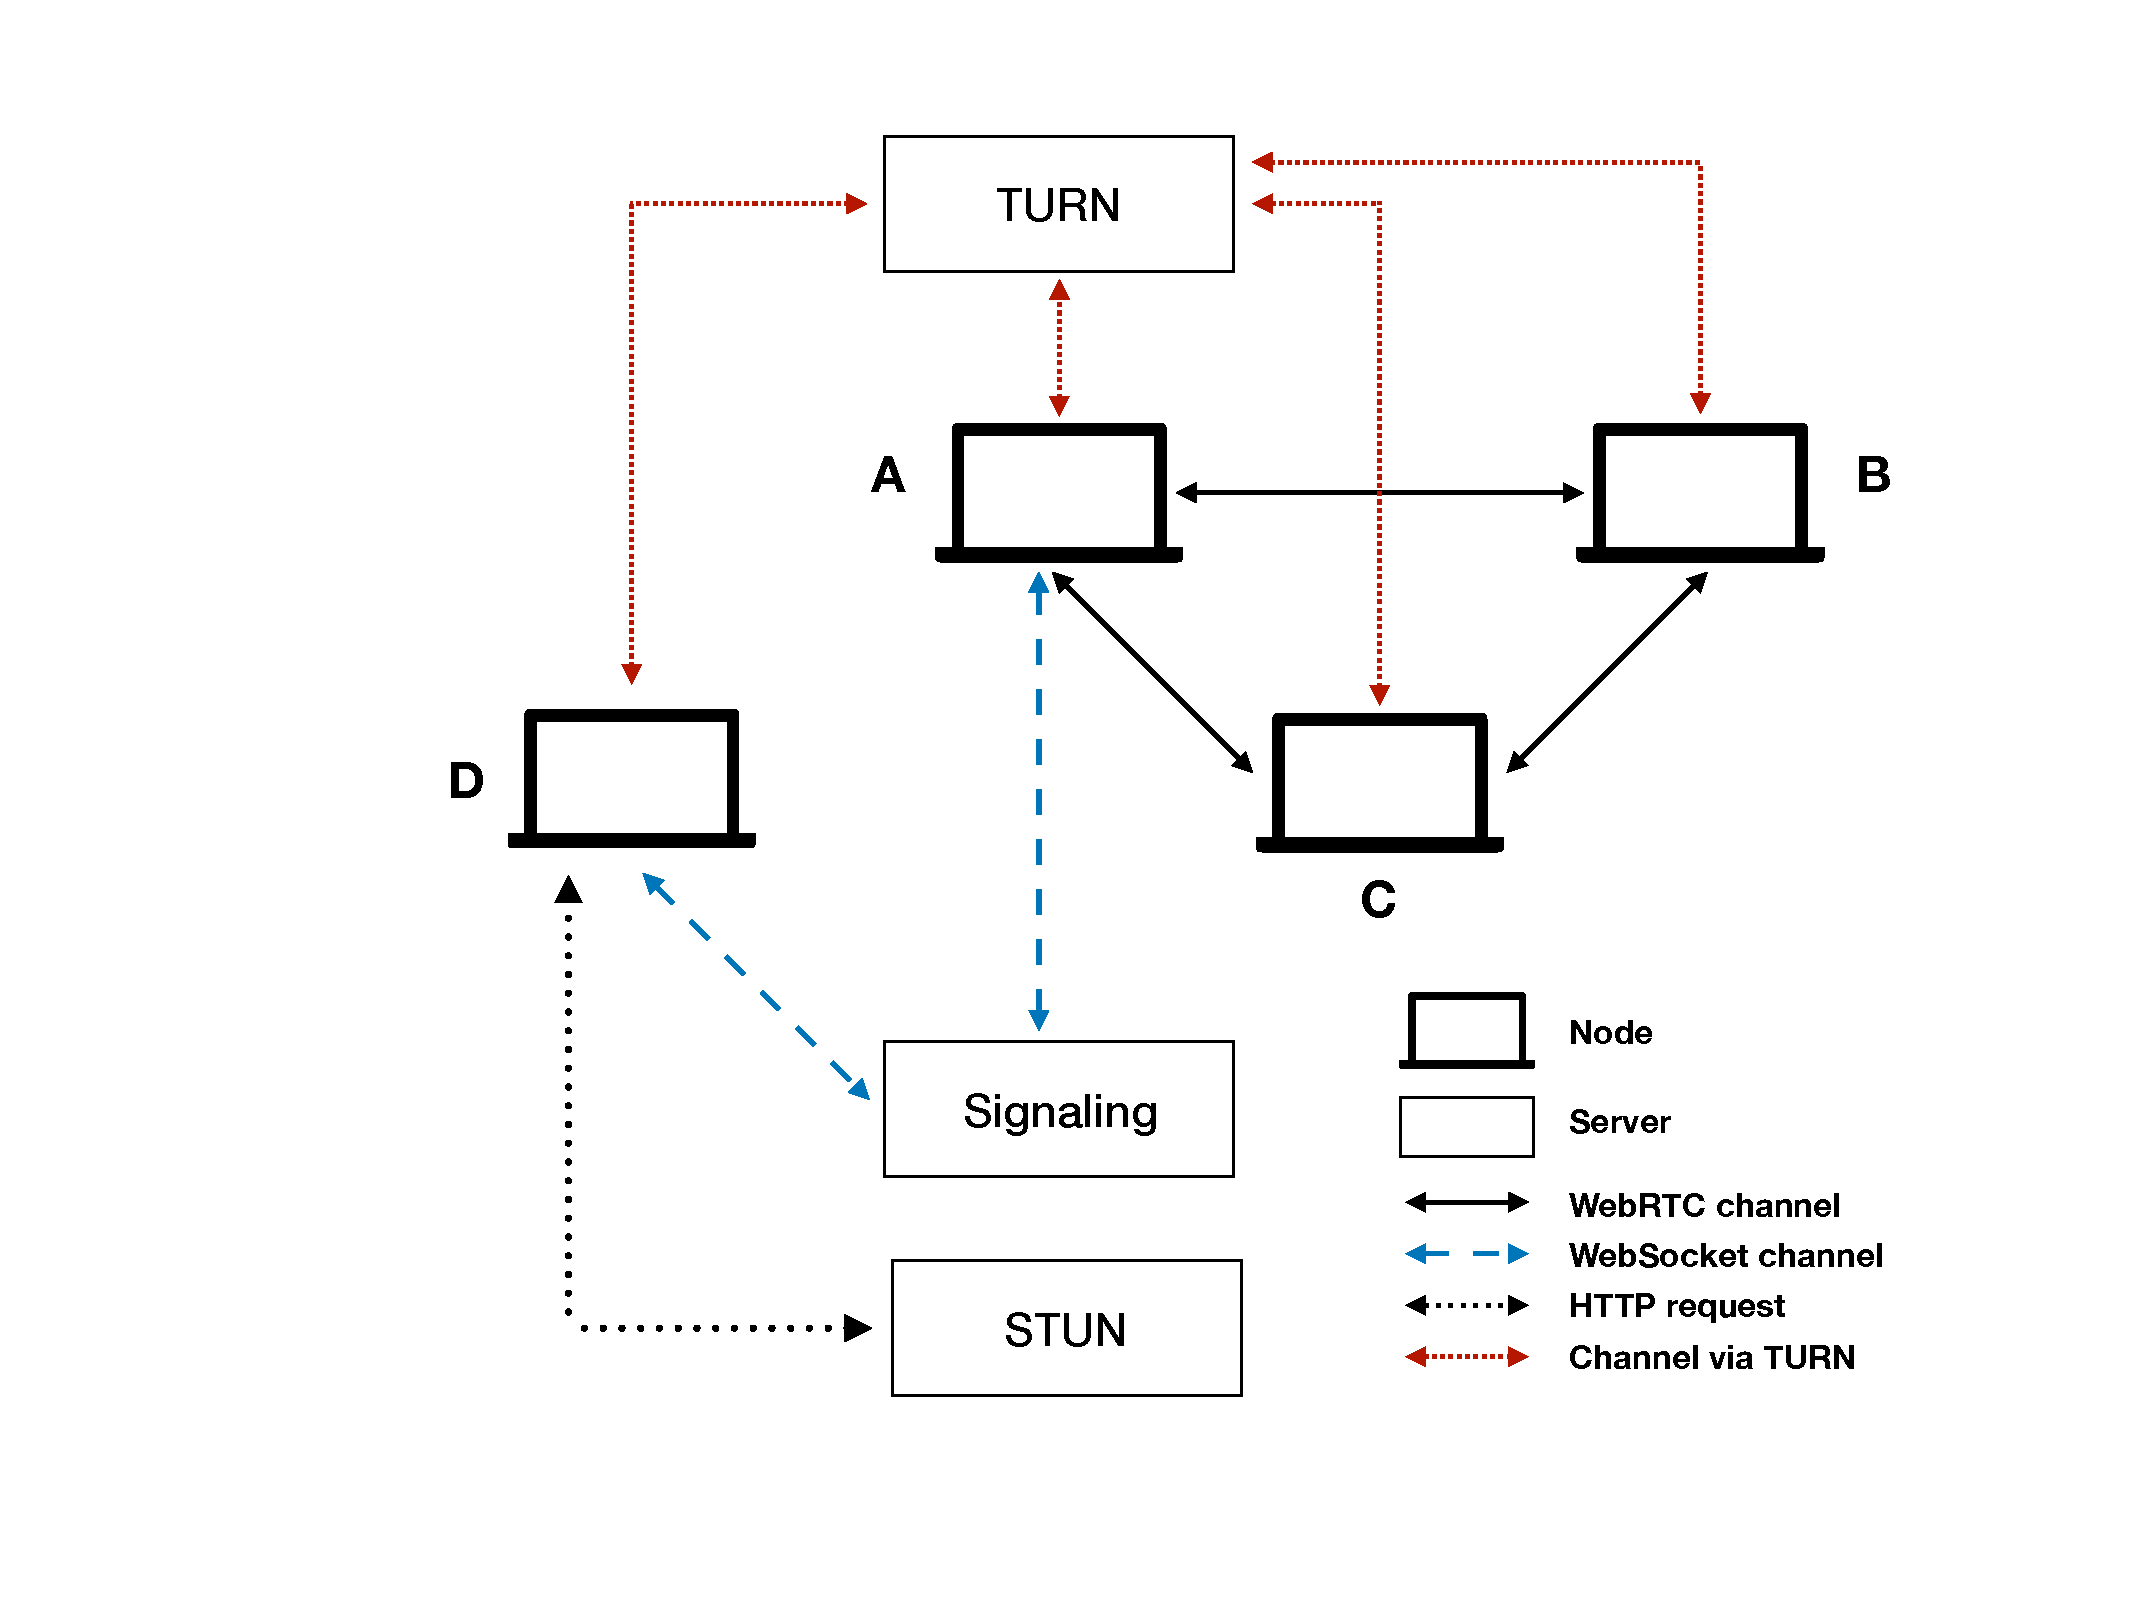
\includegraphics[page=1, trim=0cm 0cm 0cm 0cm, clip, width=.7\linewidth]{img/mute-figures.pdf}
  \caption{Architecture système de l'application MUTE}
  \label{fig:architecture-sys-mute}
\end{figure}

Nous décrivons l'architecture logicielle d'un noeud dans la \autoref{fig:architecture-log-mute}.
Dans ce chapitre, nous présentons les différentes couches logicielles de MUTE.
Notamment, nous détaillons les couches correspondantes à l'implémentation des travaux présentés dans le \autoref{chap:renamablelogootsplit}.
De la même façon, nous précisons dans ce chapitre les différents composants de l'architecture système de MUTE autre que les pairs eux-mêmes.

\begin{figure}[!ht]
  \centering
  \includegraphics[page=2, trim=0cm 0cm 0cm 0cm, clip, width=.7\linewidth]{img/mute-figures.pdf}
  \caption{Architecture logicielle de l'application MUTE}
  \label{fig:architecture-log-mute}
\end{figure}

\section{Couche interface utilisateur}

La \autoref{fig:interface-mute} illustre l'interface utilisateur de l'éditeur de document de MUTE.

\begin{figure}[!ht]
  \centering
  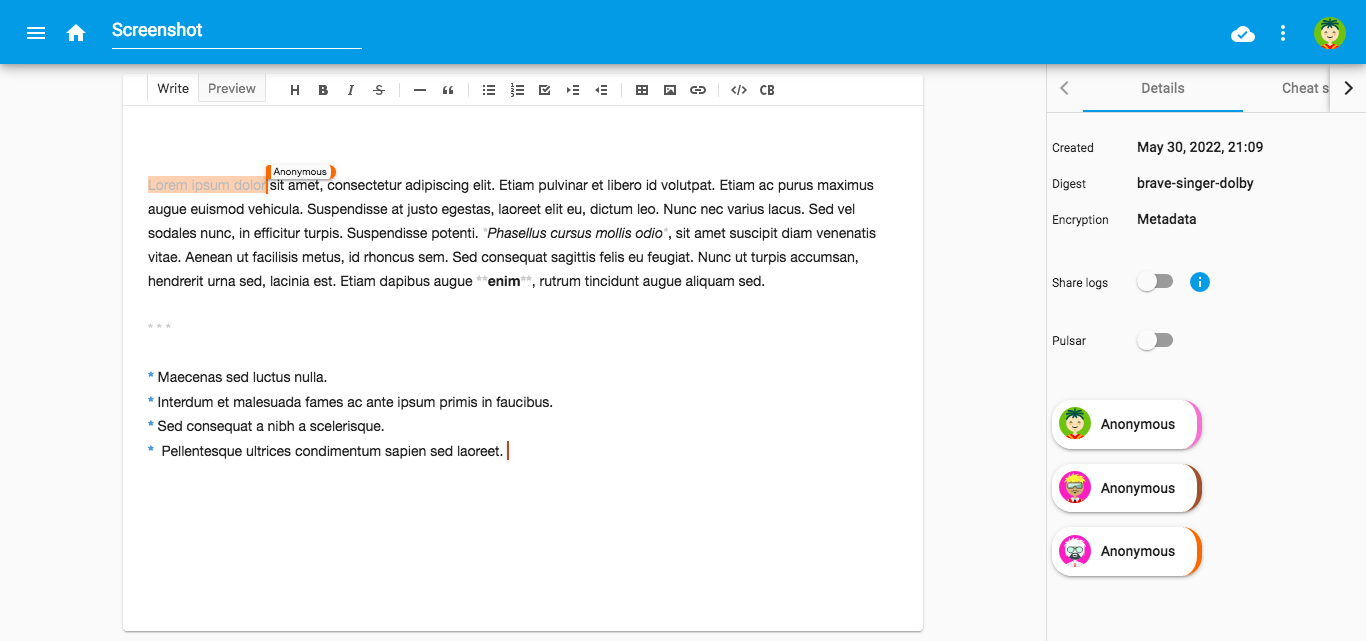
\includegraphics[width=\linewidth]{img/screenshot-mute.png}
  \caption{Capture d'écran d'une session d'édition collaborative avec MUTE}
  \label{fig:interface-mute}
\end{figure}

L'interface se compose d'un éditeur de texte supportant le langage de balisage Markdown.
Ainsi, l'éditeur permet d'inclure plusieurs éléments légers de style.
Les balises du langage Markdown étant du texte, elles sont répliquées nativement par la structure de données utilisée en interne par MUTE.

L'éditeur est agrémenté de plusieurs mécanismes permettant d'établir une conscience de groupe entre les collaborateurs.
L'indicateur en haut à droite de la fenêtre représente le statut de connexion de l'utilisateur.
Ceci lui indique s'il est actuellement connecté au réseau \ac{P2P}, en cours de connexion, ou si un incident réseau a lieu.

MUTE affiche la liste des collaborateurs actuellement connectés sur la droite de l'éditeur.
De plus, un curseur ou une sélection distante est associée à chaque collaborateur de la liste.
Elle permet d'indiquer à l'utilisateur courant dans quelles sections du document ses collaborateurs sont en train de travailler.
Ainsi, ils peuvent se répartir la rédaction du document de manière implicite ou suivre facilement les modifications d'un collaborateur.

Les documents de l'utilisateur étant sauvegardés dans le navigateur, les documents sont aussi bien disponibles en étant en ligne que hors ligne.
Une seconde page, listant les documents sauvegardés, permet à l'utilisateur de parcourir ses différents documents.

\section{Couche réplication}

\subsection{Modèle de données du document texte}

MUTE propose plusieurs alternatives pour représenter le document texte.
MUTE permet de soit utiliser une implémentation de LogootSplit\footnote{Les deux implémentations proviennent de la librairie \texttt{mute-structs} : \url{https://github.com/coast-team/mute-structs}}, soit de RenamableLogootSplit\footnotemark[\value{footnote}] ou soit de Dotted LogootSplit \footnote{Implémentation fournie par la librairie suivante : \url{https://github.com/coast-team/dotted-logootsplit}}.
Ce choix est effectué via une valeur de configuration de l'application choisie au moment de son déploiement.

Le modèle de données utilisé interagit avec l'éditeur de texte par l'intermédiaire d'opérations textes.
Lorsque l'utilisateur effectue des modifications locales, celles-ci sont détectées et mises sous la forme d'opérations textes.
Elles sont transmises au modèle de données, qui les intègre alors à la structure de données répliquées.
Le \ac{CRDT} retourne en résultat l'opération distante à propager aux autres noeuds.

De manière complémentaire, lorsqu'une opération distante est délivrée au modèle de données, elle est intégrée par le \ac{CRDT} pour actualiser son état.
Le \ac{CRDT} génère les opérations textes correspondantes et les transmet à l'éditeur de texte pour mettre à jour la vue.

En plus du texte, MUTE maintient un ensemble de métadonnées par document.
Par exemple, les utilisateurs peuvent donner un titre au document.
Pour représenter cette donnée additionnelle, nous associons un Last-Writer-Wins Register \ac{CRDT} synchronisé par opérations\cite{shapiro_2011_crdt} au document.
De façon similaire, nous utilisons un First-Writer-Wins Register \ac{CRDT} synchronisé par opérations pour représenter la date de création du document.

\subsection{Module de livraison des opérations}

Dans le cadre de LogootSplit et de RenamableLogootSplit, le modèle de données utilisé pour représenter le document texte est couplé au composant \texttt{Sync}.
Le rôle de ce composant est d'assurer le respect du modèle de livraison des opérations au \ac{CRDT}.
Pour cela, le module \texttt{Sync} doit implémenter les contraintes présentées dans la \autoref{def:ls-delivery-model} et dans la \autoref{def:rls-delivery-model}.

\subsubsection{Livraison des opérations en exactement un exemplaire}

\label{sec:mute-exactly-once-delivery}

Afin de respecter la contrainte de \emph{exactly-once delivery}, il est nécessaire d'identifier de manière unique chaque opération.
Pour cela, le module \texttt{Sync} ajoute un \emph{Dot}\cite{2014-scalable-accurate-causality-tracking} à chaque opération :

\begin{definition}[Dot]
  Un \emph{Dot} est une paire $\langle$nodeId, nodeSyncSeq$\rangle$ où
  \begin{itemize}
    \item nodeId est l'identifiant unique du noeud qui a généré l'opération.
    \item nodeSyncSeq est le numéro de séquence courant du noeud à la génération de l'opération.
  \end{itemize}
\end{definition}

Il est à noter que \emph{nodeSyncSeq} est différent du \emph{nodeSeq} utilisé dans LogootSplit et RenamableLogootSplit (cf. \autoref{def:logootsplit}).
En effet, \emph{nodeSyncSeq} se doit d'augmenter à chaque opération tandis que \emph{nodeSeq} n'augmente qu'à la création d'un nouveau bloc.
Les contraintes étant différentes, il est nécessaire de distinguer ces deux données.

Chaque noeud maintient une structure de données représentant l'ensemble des opérations reçues par le pair.
Elle permet de vérifier à la réception d'une opération si le dot de cette dernière est déjà connu.
S'il s'agit d'un nouveau dot, le module \texttt{Sync} peut délivrer l'opération au \ac{CRDT} et ajouter son dot à la structure.
Le cas échéant, cela indique que l'opération a déjà été délivrée précédemment et doit être ignorée cette fois-ci.

Plusieurs structures de données sont adaptées pour maintenir l'ensemble des opérations reçues.
Dans le cadre de MUTE, nous avons choisi d'utiliser un vecteur de versions.
Cette structure nous permet de réduire à un dot par noeud le surcoût en métadonnées du module \texttt{Sync}, puisqu'il ne nécessite que de stocker le dot le plus récent par noeud.
Cette structure permet aussi de vérifier en temps constant si une opération est déjà connue.
La \autoref{fig:exactly-once-delivery} illustre son fonctionnement.

\begin{figure}[!ht]
  \subfloat[Exécution avec livraison multiple d'une opération \emph{insert}]{
      \begin{minipage}{\linewidth}
          \centering
          \resizebox{\columnwidth}{!}{
            \begin{tikzpicture}
                \path
                    node {\textbf{A}}
                    ++(0:0.5 * \widthletter) node[epoch] {\epoch{0}}
                    ++(0:1.05 * \widthoriginepoch) node[block, label=below:{\id{p}{A0}{0..4}}] (S0A) {OGNON}
                    ++(0:5 * \widthletter) node[epoch] (S1A-left) {\epoch{0}}
                    ++(0:1.05* \widthoriginepoch) node[letter, label=below:{\id{p}{A0}{0}}]  {O}
                    ++(0:\widthletter) node[letter, fill=mydarkorange, label=above:{\id{p}{A0}{0}\id{m}{A1}{0}}] {I}
                    ++(0:\widthletter) node[block, label=below:{\id{p}{A0}{1..4}}] (S1A-right) {GNON}
                    ++(0:21 * \widthletter) node[epoch] (S2A-left) {\epoch{0}}
                    ++(0:1.05 * \widthoriginepoch) node[letter, label=below:{\id{p}{A0}{0}}] {O}
                    ++(0:\widthletter) node[block, label=below:{\id{p}{A0}{1..4}}] {GNON};


                \path
                    ++(270:4) node {\textbf{B}}
                    ++(0:0.5 * \widthletter) node[epoch] {\epoch{0}}
                    ++(0:1.05 * \widthoriginepoch) node[block, label=below:{\id{p}{A0}{0..4}}] (S0B) {OGNON}
                    ++(0:12 * \widthletter) node[epoch] (S1B-left) {\epoch{0}}
                    ++(0:1.05 * \widthoriginepoch) node[letter, label=below:{\id{p}{A0}{0}}] {O}
                    ++(0:\widthletter) node[letter, fill=mydarkorange, label=above:{\id{p}{A0}{0}\id{m}{A1}{0}}] {I}
                    ++(0:\widthletter) node[block, label=below:{\id{p}{A0}{1..4}}] (S1B-right) {GNON}
                    ++(0:5 * \widthletter) node[epoch] (S2B-left) {\epoch{0}}
                    ++(0:1.05 * \widthoriginepoch) node[letter, label=below:{\id{p}{A0}{0}}] {O}
                    ++(0:\widthletter) node[block, label=below:{\id{p}{A0}{1..4}}] (S2B-right) {GNON}
                    ++(0:8 * \widthletter) node[epoch] (S3B-left) {\epoch{0}}
                    ++(0:1.05 * \widthoriginepoch) node[letter, label=below:{\id{p}{A0}{0}}] {O}
                    ++(0:\widthletter) node[block, label=below:{\id{p}{A0}{1..4}}] {GNON};

                \draw[->, thick]
                  (S0A) edge node[above, align=center]{\emph{insert "I"}\\\emph{between}\\\emph{"O" and "G"}} (S1A-left)
                  (S1B-right) edge node[above, align=center]{\emph{remove "I"}} (S2B-left);

                \draw[dotted]
                  (S1A-right) -- (S2A-left)
                  (S0B) -- (S1B-left)
                  (S2B-right) -- (S3B-left);

                \draw[dashed, ->, thick, shorten >= 3]
                  (S1A-right.east) edge node[right, align=center]{\emph{insert "I" at} {\color{mydarkorange}\id{p}{A0}{0}\id{m}{A1}{0}}}  (S1B-left.west)
                  (S1A-right.east) edge node[right, align=center]{\emph{insert "I" at} {\color{mydarkorange}\id{p}{A0}{0}\id{m}{A1}{0}}}  (S3B-left.west)
                  (S2B-right.east) edge node[below right, align=center]{\emph{remove} {\color{mydarkorange}\id{i}{B0}{1..1}}} (S2A-left.west);
            \end{tikzpicture}
            \label{fig:exactly-once-delivery-rls}
          }
          \end{minipage}
        }
        \hfil
  \subfloat[État et comportement de la couche \texttt{Sync} au cours de l'exécution décrite en \autoref{fig:exactly-once-delivery-rls}]{
    \begin{minipage}{\linewidth}
      \centering
      \resizebox{\columnwidth}{!}{
        \begin{tikzpicture}
            \path
                node {\textbf{A}}
                ++(0:1) node[point, label=above:{$\langle A:5 \rangle$}] (a-start) {}
                ++(0:2) node[draw, circle, label=above:{$\langle A:6 \rangle$}] (a-a6) {a6}
                ++(0:8) node[point, label=above:{$\langle A:6,B:1 \rangle$}, label=below:{\emph{deliver}}] (a-b1) {}
                ++(0:3) node (a-end) {};


            \path
                ++(270:3) node {\textbf{B}}
                ++(0:1) node[point, label=below:{$\langle A:5 \rangle$}] (b-start) {}
                ++(0:5) node[point, label=below:{$\langle A:6 \rangle$}, label=above:{\emph{deliver}}] (b-a6-1) {}
                ++(0:2) node[draw, circle, label=below:{$\langle A:6,B:1 \rangle$}] (b-b1) {b1}
                ++(0:5) node[point, label=below:{$\langle A:6,B:1 \rangle$}, label=above:{\emph{discard}}] (b-a6-2) {}
                ++(0:1) node (b-end) {};

            \draw[->, thick]
              (a-start) edge (a-a6)
              (b-a6-1) edge (b-b1);

            \draw[dotted]
              (a-a6) -- (a-b1) -- (a-end)
              (b-start) -- (b-a6-1)
              (b-b1) -- (b-end);

            \draw[dashed, ->, thick, shorten >= 3]
              (a-a6.east) edge (b-a6-1.west)
              (a-a6.east) edge (b-a6-2.west)
              (b-b1.east) edge (a-b1.west);
        \end{tikzpicture}
        \label{fig:exactly-once-delivery-sync}
      }
      \end{minipage}
    }
  \caption{Gestion de la livraison \emph{exactly-once} des opérations}
  \label{fig:exactly-once-delivery}
\end{figure}

Dans cet exemple, qui reprend celui de la \autoref{fig:why-exactly-once-delivery}, deux noeuds A et B répliquent une séquence.
Initialement, celle-ci contient les éléments "OGNON".
Ces éléments ont été insérés un par un par le noeud A, donc par le biais des opérations \emph{a1} à \emph{a5}.
Le module \texttt{Sync} de chaque noeud maintient donc initialement le vecteur de version $\langle A:5 \rangle$.

Le noeud A insère l'élément "I" entre les éléments "O" et "G".
Cette modification est alors labellisée \emph{a6} par son module \texttt{Sync} et est envoyée au noeud B.
À la réception de cette opération, le module \texttt{Sync} de B compare son dot avec son vecteur de version local.
L'opération \emph{a6} étant la prochaine opération attendue de A, celle-ci est acceptée : elle est alors délivrée au \ac{CRDT} et le vecteur de version est mis à jour.

Le noeud B supprime ensuite l'élément nouvellement inséré.
S'agissant de la première modification de B, cette modification \emph{b1} ajoute l'entrée correspondante dans le vecteur de version $\langle A:6, B:1 \rangle$.
L'opération est envoyée au noeud A.
Cette opération étant la prochaine opération attendue de B, elle est acceptée et délivrée.

Finalement, le noeud B reçoit de nouveau l'opération \emph{a6}.
Son module \texttt{Sync} détermine alors qu'il s'agit d'un doublon : l'opération apparaît déjà dans le vecteur de version $\langle A:6, B:1 \rangle$.
L'opération est donc ignorée, et la résurgence de l'élément "I" illustrée dans la \autoref{fig:why-exactly-once-delivery} est évitée.

Il est à noter que dans le cas où un noeud reçoit une opération avec un dot plus élevé que celui attendu (\eg le noeud A reçoit une opération \emph{b3} à la fin de l'exemple), cette opération est mise en attente.
En effet, délivrer cette opération nécessiterait de mettre à jour le vecteur de version à $\langle A:6,B:3 \rangle$ et masquerait le fait que l'opération \emph{b2} n'a jamais été reçue.
L'opération \emph{b3} serait donc mise en attente jusqu'à la livraison de l'opération \emph{b2}.

Ainsi, l'implémentation de livraison \emph{exactly-once} avec un vecteur de version comme structure de données force une livraison \ac{FIFO} des opérations par noeuds.
Il s'agit d'une contrainte non-nécessaire et qui peut introduire des délais dans la collaboration, notamment si une opération d'un noeud est perdue par le réseau.
Nous jugeons cependant acceptable ce compromis entre le surcoût du mécanisme de livraison \emph{exactly-once} et son impact sur l'expérience utilisateur.

Pour retirer cette contrainte superflue, il est possible de remplacer cette structure de données par un \emph{Interval Version Vector} \cite{2014-optimized-or-sets}.
Au lieu d'enregistrer seulement le dernier dot observé par noeud, cette structure de données enregistre les intervalles de dots observés.
Ceci permet une livraison \emph{out of order} des opérations tout en garantissant une livraison \emph{exactly-once} et en compactant efficacement les données stockées par le module \texttt{Sync} à terme.

\subsubsection{Livraison de l'opération \emph{remove} après l'opération \emph{insert}}

La seconde contrainte que le modèle de livraison doit respecter spécifie qu'une opération \emph{remove} doit être délivrée après les opérations \emph{insert} insérant les éléments concernés.

Pour cela, le module \texttt{Sync} ajoute un ensemble \emph{Deps} à chaque opération \emph{remove} avant de la diffuser :

\begin{definition}[Deps]
  \emph{Deps} est un ensemble d'opérations.
  Il représente l'ensemble des opérations dont dépend l'opération \emph{remove} et qui doivent donc être livrées au préalable.
\end{definition}

Plusieurs structures de données sont adaptées pour représenter les dépendances de l'opération \emph{remove}.
Dans le cadre de MUTE, nous avons choisi d'utiliser un ensemble de dots : pour chaque élément supprimé par l'opération \emph{remove}, nous identifions le noeud l'ayant inséré et nous ajoutons le dot correspondant à l'opération la plus récente de ce noeud à l'ensemble des dépendances.
Cette approche nous permet de limiter à un dot par élément supprimé le surcoût en métadonnées des dépendances et de les calculer en un temps linéaire par rapport au nombre d'éléments supprimés.
Nous illustrons le calcul et l'utilisation des dépendances de l'opération \emph{remove} à l'aide de la \autoref{fig:causal-remove-delivery}.

\begin{figure}[!ht]
  \subfloat[Exécution avec livraison dans le désordre d'une insertion et de sa suppression]{
      \begin{minipage}{\linewidth}
          \centering
          \resizebox{\columnwidth}{!}{
            \begin{tikzpicture}
              \path
                  node {\textbf{A}}
                  ++(0:0.5 * \widthletter) node[epoch] {\epoch{0}}
                  ++(0:1.05 * \widthoriginepoch) node[block, label=below:{\id{p}{A0}{0..4}}] (S0A) {OGNON}
                  ++(0:5 * \widthletter) node[epoch] (S1A-left) {\epoch{0}}
                  ++(0:1.05* \widthoriginepoch) node[letter, label=below:{\id{p}{A0}{0}}]  {O}
                  ++(0:\widthletter) node[letter, fill=mydarkorange, label=above:{\id{p}{A0}{0}\id{m}{A1}{0}}] {I}
                  ++(0:\widthletter) node[block, label=below:{\id{p}{A0}{1..4}}] (S1A-right) {GNON}
                  ++(0:21 * \widthletter) node[epoch] (S2A-left) {\epoch{0}}
                  ++(0:1.05 * \widthoriginepoch) node[letter, label=below:{\id{p}{A0}{0}}] {O}
                  ++(0:\widthletter) node[block, label=below:{\id{p}{A0}{1..4}}] (S2A-right) {GNON}
                  ++(0:19 * \widthletter) node (A-end) {};


              \path
                  ++(270:4) node {\textbf{B}}
                  ++(0:0.5 * \widthletter) node[epoch] {\epoch{0}}
                  ++(0:1.05 * \widthoriginepoch) node[block, label=below:{\id{p}{A0}{0..4}}] (S0B) {OGNON}
                  ++(0:12 * \widthletter) node[epoch] (S1B-left) {\epoch{0}}
                  ++(0:1.05 * \widthoriginepoch) node[letter, label=below:{\id{p}{A0}{0}}] {O}
                  ++(0:\widthletter) node[letter, fill=mydarkorange, label=above:{\id{p}{A0}{0}\id{m}{A1}{0}}] {I}
                  ++(0:\widthletter) node[block, label=below:{\id{p}{A0}{1..4}}] (S1B-right) {GNON}
                  ++(0:5 * \widthletter) node[epoch] (S2B-left) {\epoch{0}}
                  ++(0:1.05 * \widthoriginepoch) node[letter, label=below:{\id{p}{A0}{0}}] {O}
                  ++(0:\widthletter) node[block, label=below:{\id{p}{A0}{1..4}}] (S2B-right) {GNON}
                  ++(0:29 * \widthletter) node (B-end) {};

              \path
                  ++(270:8) node {\textbf{C}}
                  ++(0:\widthletter) node[epoch] {\epoch{0}}
                  ++(0:1.05 * \widthoriginepoch) node[block, label=below:{\id{p}{A0}{0..4}}] (S0C) {OGNON}
                  ++(0:30 * \widthletter) node[point] (S1C) {}
                  ++(0:8 * \widthletter) node[letter, label=below:{\id{p}{A0}{0}}] (S2C-left) {O}
                  ++(0:\widthletter) node[letter, fill=mydarkorange, label=above:{\id{p}{A0}{0}\id{m}{A1}{0}}] {I}
                  ++(0:\widthletter) node[block, label=below:{\id{p}{A0}{1..4}}] (S2C-right) {GNON}
                  ++(0:5 * \widthletter) node[epoch] (S3C-left) {\epoch{0}}
                  ++(0:1.05 * \widthoriginepoch) node[letter, label=below:{\id{p}{A0}{0}}] {O}
                  ++(0:\widthletter) node[block, label=below:{\id{p}{A0}{1..4}}] (S3C-right) {GNON}
                  ++(0:2 * \widthblock) node (C-end) {};

              \draw[->, thick]
                (S0A) edge node[above, align=center]{\emph{insert "I"}\\\emph{between}\\\emph{"O" and "G"}} (S1A-left)
                (S1B-right) edge node[above, align=center]{\emph{remove "I"}} (S2B-left);

              \draw[dotted]
                (S1A-right) -- (S2A-left)
                (S2A-right) -- (A-end)
                (S0B) -- (S1B-left)
                (S2B-right) -- (B-end)
                (S0C) -- (S1C)
                (S1C) -- (S2C-left)
                (S2C-right) -- (S3C-left)
                (S3C-right) -- (C-end);

              \draw[dashed, ->, thick, shorten >= 3]
                (S1A-right.east) edge node[right, align=center]{\emph{insert "I" at} {\color{mydarkorange}\id{p}{A0}{0}\id{m}{A1}{0}}}  (S1B-left.west)
                (S1A-right.east) edge node[pos=0.85, right, align=center]{\emph{insert "I" at} {\color{mydarkorange}\id{p}{A0}{0}\id{m}{A1}{0}}}  (S2C-left.west)
                (S2B-right.east) edge node[below right, align=center]{\emph{remove} {\color{mydarkorange}\id{i}{B0}{1..1}}} (S2A-left.west)
                (S2B-right.east) edge node[pos=0.80, right, align=center]{\emph{remove} {\color{mydarkorange}\id{i}{B0}{1..1}}} (S1C.west);

              \draw[->, dashed, thick, shorten >= 3] (S1C.east) edge[bend left] (S3C-left.west);
            \end{tikzpicture}
            \label{fig:causal-remove-delivery-rls}
          }
          \end{minipage}
        }
        \hfil
  \subfloat[État et comportement de la couche \texttt{Sync} au cours de l'exécution décrite en \autoref{fig:causal-remove-delivery-rls}]{
    \begin{minipage}{\linewidth}
      \centering
      \resizebox{\columnwidth}{!}{
        \begin{tikzpicture}
            \path
                node {\textbf{A}}
                ++(0:1) node[point, label=above:{$\langle A:5 \rangle$}] (a-start) {}
                ++(0:2) node[draw, circle, label=above:{$\langle A:6 \rangle$}] (a-a6) {a6}
                ++(0:8) node[point, label=above:{$\langle A:6,B:1 \rangle$}, label=below:{\emph{deliver}}] (a-b1) {}
                ++(0:11) node (a-end) {};


            \path
                ++(270:3) node {\textbf{B}}
                ++(0:1) node[point, label=below:{$\langle A:5 \rangle$}] (b-start) {}
                ++(0:5) node[point, label=below:{$\langle A:6 \rangle$}, label=above:{\emph{deliver}}] (b-a6) {}
                ++(0:2) node[draw, circle, label=below:{$\langle A:6,B:1 \rangle$}] (b-b1) {b1}
                ++(0:14) node (b-end) {};

            \path
                ++(270:6) node {\textbf{C}}
                ++(0:1) node[point, label=below:{$\langle A:5 \rangle$}] (c-start) {}
                ++(0:10) node[point, label=below:{$\langle A:5 \rangle$}, label=above:{\emph{postpone}}] (c-b1-postpone) {}
                ++(0:5) node[point, label=below:{$\langle A:6 \rangle$}, label=above:{\emph{deliver}}] (c-a6) {}
                ++ (0:5) node[point, label=below:{$\langle A:6,B:1 \rangle$}, label=above:{\emph{deliver}}] (c-b1-deliver) {}
                ++(0:1) node (c-end) {};

            \draw[->, thick]
              (a-start) edge (a-a6)
              (b-a6-1) edge (b-b1);

            \draw[dotted]
              (a-a6) -- (a-b1) -- (a-end)
              (b-start) -- (b-a6)
              (b-b1) -- (b-end)
              (c-start) -- (c-b1-postpone)
              (c-b1-postpone) -- (c-a6)
              (c-a6) -- (c-b1-deliver)
              (c-b1-deliver) -- (c-end);

            \draw[dashed, ->, thick, shorten >= 3]
              (a-a6.east) edge (b-a6.west)
              (b-b1.east) edge node[right] {$\{\trm{deps}: \langle A:6 \rangle\}$} (a-b1.west)
              (b-b1.east) edge node[right] {$\{\trm{deps}: \langle A:6 \rangle\}$} (c-b1-postpone.west)
              (a-a6.east) edge (c-a6.west);

            \draw[->, dashed, thick, shorten >= 3] (c-b1-postpone.east) edge[bend left] (c-b1-deliver.west);
        \end{tikzpicture}
        \label{fig:causal-remove-sync}
      }
      \end{minipage}
    }
  \caption{Gestion de la livraison \emph{causale-remove} des opérations}
  \label{fig:causal-remove-delivery}
\end{figure}

Cet exemple reprend et complète celui de la \autoref{fig:causal-remove-delivery}.
Trois noeuds A, B et C répliquent et éditent collaborativement une séquence.
Les trois noeuds partagent le même état initial : une séquence contenant les éléments "OGNON" et un vecteur de version $\langle A:5 \rangle$.

Le noeud A insère l'élément "I" entre les éléments "O" et "G".
Cet élément se voit attribué l'identifiant \id{p}{A0}{0}\id{m}{A1}{0}.
L'opération correspondante \emph{a6} est diffusée aux autres noeuds.

À la réception de cette dernière, le noeud B supprime l'élément "I" nouvellement inséré et génère l'opération \emph{b1} correspondante.
Comme indiqué précédemment, l'opération \emph{b1} étant une opération \emph{remove}, le module \texttt{Sync} calcule ses dépendances avant de la diffuser.
Pour chaque élément supprimé ("I"), \texttt{Sync} récupère l'identifiant de l'élément (\id{p}{A0}{0}\id{m}{A1}{0}) et en extrait l'identifiant du noeud qui l'a inséré (A).
\texttt{Sync} ajoute alors le dot de l'opération la plus récente reçue de ce noeud ($\langle A:6 \rangle$) à l'ensemble des dépendances de l'opération.
L'opération est ensuite diffusée.

À la réception de l'opération \emph{b1}, le noeud A vérifie s'il possède l'ensemble des dépendances de l'opération.
Le noeud A ayant déjà observé l'opération \emph{a6}, le module \texttt{Sync} délivre l'opération \emph{b1} au \ac{CRDT}.

À l'inverse, lorsque le noeud C reçoit l'opération \emph{b1}, il n'a pas encore reçu l'opération \emph{a6}.
L'opération \emph{b1} est alors mise en attente.
À la réception de l'opération \emph{a6}, celle-ci est délivrée.
Le module \texttt{Sync} ré-évalue alors le cas de l'opération \emph{b1} et détermine qu'elle peut à présent être délivrée.

Il est à noter que notre approche pour générer l'ensemble des dépendances est une approximation.
En effet, nous ajoutons les dots des opérations les plus récentes des auteurs des éléments supprimés.
Nous n'ajoutons pas les dots des opérations qui ont spécifiquement insérés les éléments supprimés.
Pour cela, il serait nécessaire de parcourir le log des opérations à la recherche des opérations \emph{insert} correspondante.
Cette méthode serait plus coûteuse, sa complexité dépendant du nombre d'opérations dans le log d'opérations, et incompatible avec un mécanisme tronquant le log des opérations en utilisant la stabilité causale.
Notre approche introduit un potentiel délai dans la livraison d'une opération \emph{remove} par rapport à une livraison utilisant ses dépendances exactes, puisqu'elle va reposer sur des opérations plus récentes et potentiellement encore inconnues par le noeud.
Mais il s'agit là aussi d'un compromis que nous jugeons acceptable entre le surcoût du mécanisme de livraison et l'expérience utilisateur.

\subsubsection{Livraison des opérations après l'opération \emph{rename} introduisant leur époque}

La troisième contrainte spécifiée par le modèle de livraison est qu'une opération doit être délivrée après l'opération \emph{rename} qui a introduite son époque de génération.

Pour cela, le module \texttt{Sync} doit donc récupérer l'époque courante de la séquence répliquée, récupérer le dot de l'opération \emph{rename} l'ayant introduite et l'ajouter en tant que dépendance de chaque opération.
Cependant, dans notre implémentation, le module \texttt{Sync} et le module représentant la séquence répliquée sont découplés et ne peuvent interagir directement l'un avec l'autre.

Pour remédier à ce problème, le module \texttt{Sync} maintient une structure supplémentaire : un vecteur des dots des opérations \emph{rename} connues.
À la réception d'une opération \emph{rename} distante, l'entrée correspondante de son auteur est mise à jour avec le dot de la nouvelle époque introduite.
À la génération d'une opération locale, l'opération est examinée pour récupérer son époque de génération.
\texttt{Sync} conserve alors seulement l'entrée correspondante dans le vecteur des dots des opérations \emph{rename}.
À ce stade, le contenu du vecteur est ajouté en tant que dépendance de l'opération.
Ensuite, si l'opération locale s'avère être une opération \emph{rename}, le vecteur est modifié pour ne conserver que le dot de l'époque introduite par l'opération.
La \autoref{fig:epoch-based-delivery} illustre ce fonctionnement.

\begin{figure}[!ht]
  \subfloat[Exécution]{
      \begin{minipage}{\linewidth}
          \centering
          \resizebox{\columnwidth}{!}{
            \begin{tikzpicture}
              \path
                node {\textbf{A}}
                +(0:20) node (a-end) {}
                ++(0:0.5) node (a0) {}
                ++(0:3) node[point, label=above:{rename to \epoch{A1}}] (a1) {}
                ++(0:3) node [point, label=above:{rename to \epoch{A7}}] (a7) {}
                ++(0:10) node (a-receives-c1) {}
                ++(0:2) node (a-receives-b3) {};


              \draw[thick] (a0) --  (a1) -- (a7) edge (a-receives-c1) edge (a-receives-b3) edge (a-end);

              \path
                  ++(270:2) node {\textbf{B}}
                  +(0:20) node (b-end) {}
                  ++(0:0.5) node (b0) {}
                  ++(0:3) node[point, label=above:{rename to \epoch{B3}}] (b3) {};

              \draw[thick] (b0) -- (b3) -- (b-end);

              \path
                  ++(270:4) node {\textbf{C}}
                  +(0:20) node (c-end) {}
                  ++(0:0.5) node (c0) {}
                  ++(0:5.5) node (c-receives-b3) {}
                  ++(0:2.5) node (c-receives-a1) {}
                  ++(0:3) node (c-receives-a7) {}
                  ++(0:3) node[point, label=below:{insert}] (c1) {};

              \draw[thick] (c0) edge (c-receives-b3) edge (c-receives-a1) edge (c-receives-a7) -- (c1) -- (c-end);

              \draw[->, dashed, shorten >= 1]
                (a1) edge (c-receives-a1)
                (a7) edge (c-receives-a7)
                (b3) edge (a-receives-b3)
                (b3) edge (c-receives-b3)
                (c1) edge (a-receives-c1);
            \end{tikzpicture}
            \label{fig:epoch-based-delivery-execution}
          }
          \end{minipage}
        }
        \hfil
  \subfloat[État et comportement de la couche \texttt{Sync} au cours de l'exécution décrite en \autoref{fig:epoch-based-delivery-execution}]{
    \begin{minipage}{\linewidth}
      \centering
      \resizebox{\columnwidth}{!}{
        \begin{tikzpicture}
          \path
            node {\textbf{A}}
            +(0:25) node (a-end) {}
            ++(0:0.5) node (a0) {}
            ++(0:3) node[op, label=above:{$\langle A:1 \rangle$}] (a1) {a1}
            ++(0:3) node [op, label=above:{$\langle A:7 \rangle$}] (a7) {a7}
            ++(0:10) node[point, label=above:{$\langle A:7 \rangle$}, label=below:{\emph{postpone}}] (a-receives-c1-postpone) {}
            ++(0:3) node[point, label=above:{$\langle A:7,B:3 \rangle$}, label=below:{\emph{deliver}}] (a-receives-b3) {}
            ++(0:3) node[point, label=above:{$\langle A:7,B:3 \rangle$}, label=below:{\emph{deliver}}] (a-receives-c1-deliver) {};


          \draw[thick] (a0) --  (a1) -- (a7) -- (a-receives-c1-postpone) -- (a-receives-b3) -- (a-receives-c1-deliver) -- (a-end);

          \path
              ++(270:2) node {\textbf{B}}
              +(0:25) node (b-end) {}
              ++(0:0.5) node (b0) {}
              ++(0:3) node[op, label=above:{$\langle B:3 \rangle$}] (b3) {b3};

          \draw[thick] (b0) -- (b3) -- (b-end);

          \path
              ++(270:4) node {\textbf{C}}
              +(0:25) node (c-end) {}
              ++(0:0.5) node (c0) {}
              ++(0:5.5) node[point, label=below:{$\langle B:3 \rangle$}, label=above:{\emph{deliver}}] (c-receives-b3) {}
              ++(0:2.5) node[point, label=below:{$\langle A:1,B:3 \rangle$}, label=above:{\emph{deliver}}] (c-receives-a1) {}
              ++(0:3) node[point, label=below:{$\langle A:7,B:3 \rangle$}, label=above:{\emph{deliver}}] (c-receives-a7) {}
              ++(0:3) node[op, label=below:{$\langle B:3 \rangle$}] (c1) {c1};

          \draw[thick] (c0) -- (c-receives-b3) -- (c-receives-a1) -- (c-receives-a7) -- (c1) -- (c-end);

          \draw[->, dashed, shorten >= 1]
            (a1.east) edge (c-receives-a1.west)
            (a7.east) edge node[near end, above right] {$\{\trm{deps}: \{\langle A:1 \rangle\}\}$} (c-receives-a7.west)
            (b3.east) edge (a-receives-b3.west)
            (b3.east) edge (c-receives-b3.west)
            (c1.east) edge node[near start, right] {$\{\trm{deps}: \{\langle B:3 \rangle\}\}$} (a-receives-c1-postpone.west);

          \draw[->, dashed, thick, shorten >= 3] (a-receives-c1-postpone.east) edge[bend right] (a-receives-c1-deliver.west);
        \end{tikzpicture}
        \label{fig:epoch-based-delivery-sync}
      }
      \end{minipage}
    }
  \caption{Gestion de la livraison \emph{epoch based} des opérations}
  \label{fig:epoch-based-delivery}
\end{figure}

Dans la \autoref{fig:epoch-based-delivery-execution}, nous décrivons une exécution suivante en ne faisant apparaître que les opérations importantes : les opérations \emph{rename} et une opération \emph{insert} finale.
Dans cette exécution, trois noeuds A, B et C répliquent et éditent collaborativement une séquence.
Initialement, aucune opération \emph{rename} n'a encore eu lieu.
Le noeud A effectue une première opération \emph{rename} (\emph{a1}) puis une seconde opération \emph{rename} (\emph{a7}), et les diffuse.
En concurrence, le noeud B génère et propage sa propre opération \emph{rename} (\emph{b3}).
De son côté, le noeud C reçoit les opérations \emph{b3}, puis \emph{a1} et \emph{a7}.
Il émet ensuite une opération \emph{insert} (\emph{c1}).
Le noeud A reçoit cette opération avant de finalement recevoir l'opération \emph{b3}.

Dans la \autoref{fig:epoch-based-delivery-sync}, nous faisons apparaître l'état de \texttt{Sync} et les décisions prises par ce dernier au cours de l'exécution.
Initialement, le vecteur des dots des opérations \emph{rename} connues est vide.
Ainsi, lorsque A génère l'opération \emph{a1}, celle-ci ne se voit ajouter aucune dépendance (nous ne représentons pas les dépendances des opérations qui correspondent à l'ensemble vide).
A met ensuite à jour son vecteur des dots des opérations \emph{rename} avec le dot $\langle A:1 \rangle$.
B procède de manière similaire avec l'opération \emph{b3}.

Quand A génère l'opération \emph{a7}, le dot $\langle A:1 \rangle$ est ajouté en tant que dépendance.
Le dot $\langle A:7 \rangle$ remplace ensuite ce dernier dans le vecteur des dots des opérations \emph{rename}.

À la réception de l'opération \emph{b3}, le module \texttt{Sync} de C peut la délivrer au \ac{CRDT}, l'ensemble de ses dépendances étant vérifié.
Le noeud C ajoute alors à son vecteur des dots des opérations \emph{rename} le dot $\langle B:3 \rangle$.
Il procède de même pour l'opération \emph{a1} : il la délivre et ajoute le dot $\langle A:1 \rangle$.
Le module \texttt{Sync} ne connaissant pas l'époque courante de la séquence répliquée, il maintient les deux dots localement.

Lorsque le noeud C reçoit l'opération \emph{a7}, l'ensemble de ses contraintes est vérifié : l'opération \emph{a1} a été délivrée précédemment.
L'opération est donc délivrée et le vecteur de dots des opérations \emph{rename} mis à jour avec $\langle A:7 \rangle$.

Quand le noeud C effectue l'opération locale \emph{c1}, le module \texttt{Sync} obtient l'information de l'époque courante de la séquence : \epoch{b3}.
C met à jour son vecteur de dots des opérations \emph{rename} pour ne conserver que l'entrée du noeud B : $\langle B:3 \rangle$.
Ce dot est ajouté en tant que dépendance de l'opération \emph{c1} avant sa diffusion.

À la réception de l'opération \emph{c1} par le noeud A, cette opération est mise en attente par \texttt{Sync}, l'opération \emph{b3} n'ayant pas encore été délivrée.
Le noeud reçoit ensuite l'opération \emph{b3}.
Son vecteur des dots des opérations \emph{rename} est mis à jour et l'opération délivrée.
Les conditions pour l'opération \emph{c1} étant désormais remplies, l'opération est alors délivrée.

Cette implémentation de la contrainte de la livraison \emph{epoch-based} dispose de plusieurs avantages : sa complexité spatiale dépend linéairement du nombre de noeuds et les opérations de mise à jour du vecteur des dots des opérations \emph{rename} s'effectuent en temps constant.
De plus, seul un dot est ajouté en tant que dépendance des opérations, la taille du vecteur des dots étant ramené à 1 au préalable.
Finalement, cette implémentation ne contraint pas une livraison causale des opérations \emph{rename} et permet donc de les appliquer dès que possible.

\subsubsection{Livraison des opérations à terme}

\label{sec:mute-anti-entropy}

La dernière contrainte du modèle de livraison précise que toutes les opérations doivent être délivrées à tous les noeuds à terme.
Cependant, le réseau étant non-fiable, des messages peuvent être perdus au cours de l'exécution.
Il est donc nécessaire que les noeuds rediffusent les messages perdus pour assurer leur livraison à terme.

Pour cela, nous implémentons un mécanisme d'anti-entropie basé sur \cite{1983-anti-entropy-vv}.
Ce mécanisme permet à un noeud source de se synchroniser avec un autre noeud cible.
Il est executé par l'ensemble des noeuds de manière indépendante.
Nous décrivons ci-dessous son fonctionnement.

De manière périodique, le noeud choisit un autre noeud cible de manière aléatoire.
Le noeud source lui envoie alors une représentation de son état courant, \ie son vecteur de version.

À la réception de ce message, le noeud cible compare le vecteur de version reçu par rapport à son propre vecteur de version.
À partir de ces données, il identifie les dots des opérations de sa connaissance qui sont inconnues au noeud source.
Grâce à leur dot, le noeud cible retrouve ces opérations depuis son log des opérations.
Il envoie alors une réponse composée de ces opérations au noeud source.

À la réception de la réponse, le noeud source intègre normalement les opérations reçues.
La \autoref{fig:anti-entropy} illustre ce mécanisme.

\begin{figure}[!ht]
  \centering
  \resizebox{\columnwidth}{!}{
    \begin{tikzpicture}
      \path
        node {\textbf{A}}
        +(0:37) node (a-end) {}
        ++(0:0.5) node (a0) {}
        ++(0:3) node[op, label=above:{$\langle A:8,B:3,C:1 \rangle$}] (a8) {a8}
        ++(0:6) node [op, label=above:{$\langle A:9,B:3,C:1 \rangle$}] (a9) {a9}
        ++(0:15) node[point, label=above:{$\langle A:9,B:4,C:1 \rangle$}, label=below:{\emph{deliver}}] (a-receives-b4) {};


      \draw[thick] (a0) --  (a8) -- (a9) -- (a-receives-b4) -- (a-end);

      \path
          ++(270:2) node {\textbf{B}}
          +(0:37) node (b-end) {}
          ++(0:0.5) node (b0) {}
          ++(0:9) node[point, label=below:{$\langle A:8,B:3,C:1 \rangle$}, label=above:{\emph{deliver}}] (b-receives-a8) {}
          ++(0:6) node[point, label=below:{$\langle A:9,B:3,C:1 \rangle$}, label=above:{\emph{deliver}}](b-receives-a9) {}
          ++(0:4) node[op, label=above:{$\langle A:9,B:4,C:1 \rangle$}] (b4) {b4}
          ++(0:12) node[point, label=above:{\emph{reply to sync query}}] (b-receives-c-sync-request) {};

      \draw[thick] (b0) -- (b-receives-a8) -- (b-receives-a9) -- (b4) -- (b-receives-c-sync-request) -- (b-end);

      \path
          ++(270:4) node {\textbf{C}}
          +(0:37) node (c-end) {}
          ++(0:0.5) node (c0) {}
          ++(0:8) node (c-receives-a8) {}
          +(90:0.5) node[cross] (fail-a8) {}
          ++(0:6) node (c-receives-a9) {}
          +(90:0.5) node[cross] (fail-a9) {}
          ++(0:10) node[point, label=below:{$\langle A:7,B:4,C:1 \rangle$}, label=above:{\emph{deliver}}] (c-receives-b4) {}
          ++(0:4) node[op, label=below:{$\langle A:7,B:4,C:1 \rangle$}] (c-query-sync) {sync}
          ++(0:6) node[point, label=below:{$\langle A:9,B:4,C:1 \rangle$}, label=above:{\emph{deliver}}] (c-receives-b-sync-reply) {};


      \draw[thick] (c0) -- (c-receives-b4) -- (c-query-sync) --  (c-receives-b-sync-reply) -- (c-end);

      \draw[->, dashed, shorten >= 1]
        (a8.east) edge (b-receives-a8.west)
        (a8.east) edge (fail-a8)
        (a9.east) edge (b-receives-a9.west)
        (a9.east) edge (fail-a9)
        (b4.east) edge (a-receives-b4.west)
        (b4.east) edge (c-receives-b4.west)
        (b-receives-c-sync-request.east) edge (c-receives-b-sync-reply.west)
        (c-query-sync.east) edge (b-receives-c-sync-request.west);

    \end{tikzpicture}
  }
  \caption{Utilisation du mécanisme d'anti-entropie par le noeud C pour se synchroniser avec le noeud B}
  \label{fig:anti-entropy}
\end{figure}

Dans cette figure, nous représentons une exécution à laquelle participent trois noeuds : A, B et C.
Initialement, les trois noeuds sont synchronisés.
Leur vecteurs de version sont identiques et ont pour valeur $\langle A:7,B:3,C:1 \rangle$.

Le noeud A effectue les opérations \emph{a8} puis \emph{a9} et les diffusent sur le réseau.
Le noeud B reçoit ces opérations et les délivre à son \ac{CRDT}.
Il effectue ensuite et propage l'opération \emph{b4}, qui est reçue et délivrée par A.
Ils atteignent tous deux la version représenté par le vecteur $\langle A:9,B:4,C:1 \rangle$

De son côté, le noeud C ne reçoit pas les opérations \emph{a8} et \emph{a9} à cause d'une défaillance réseau.
Néanmoins, cela ne l'empêche pas de délivrer l'opération \emph{b4} à sa réception et d'obtenir la version $\langle A:7,B:4,C:1 \rangle$.

Le noeud C déclenche ensuite son mécanisme d'anti-entropie.
Il choisit aléatoirement le noeud B comme noeud cible.
Il lui envoie un message de synchronisation avec pour contenu le vecteur de version $\langle A:7,B:8,C:1 \rangle$.

À la réception de ce message, le noeud B compare ce vecteur avec le sien.
Il détermine que le noeud C n'a pas reçu les opérations \emph{a8} et \emph{a9}.
B les récupère depuis son log des opérations et les envoie à C par le biais d'un nouveau message.

À la réception de la réponse de B, le noeud C délivre les opérations \emph{a8} et \emph{a9}.
Il atteint alors le même état que A et B, représenté par le vecteur de version $\langle A:9,B:4,C:1 \rangle$.

Ce mécanisme d'anti-entropie nous permet ainsi de garantir la livraison à terme de toutes les opérations et de compenser les défaillances du réseau.
Il nous sert aussi de mécanisme de synchronisation : à la connexion d'un pair, celui-ci utilise ce mécanisme pour récupérer les opérations effectuées depuis sa dernière connexion.
Dans le cas où il s'agit de la première connexion du pair, il lui suffit d'envoyer un vecteur de version vide pour récupérer l'intégralité des opérations.

Ce mécanisme propose plusieurs avantages.
Son exécution n'implique que le noeud source et le noeud cible, ce qui limite les coûts de coordination.
De plus, si une défaillance a lieu lors de l'exécution du mécanisme (perte d'un des messages, panne du noeud cible...), cette défaillance n'est pas critique : le noeud source se synchronisera à la prochaine exécution du mécanisme.
Ensuite, ce mécanisme réutilise le vecteur de version déjà nécessaire pour la livraison \emph{exactly-once}, comme présenté en \autoref{sec:mute-exactly-once-delivery}.
Il ne nécessite donc pas de stocker une nouvelle structure de données pour détecter les différences entre noeuds.

En contrepartie, la principale limite de ce mécanisme d'anti-entropie est qu'il nécessite de maintenir et de parcourir périodiquement le log des opérations pour répondre aux requêtes de synchronisation.
La complexité spatiale et en temps du mécanisme dépend donc linéairement du nombre d'opérations.
Qui plus est, nous sommes dans l'incapacité de tronquer le log des opérations en se basant sur la stabilité causale des opérations puisque nous utilisons ce mécanisme pour mettre à niveau les nouveaux pairs.
À moins de mettre en place un mécanisme de compression du log comme évoqué en \autoref{sec:rename-as-compression-mechanism}, ce log des opérations croit de manière monotone.
Néanmoins, une alternative possible est de mettre en place un système de chargement différé des opérations pour ne pas surcharger la mémoire.

\subsection{Collaborateurs}

Pour assurer la qualité de la collaboration même à distance, il est important d'offrir des fonctionnalités de conscience de groupe aux utilisateurs.
Une de ces fonctionnalités est de fournir la liste des collaborateurs actuellement connectés.
Les protocoles d'appartenance au réseau sont une catégorie de protocoles spécifiquement dédiée à cet effet.
Ainsi, nous devions en implémenter un dans MUTE.

MUTE présente cependant plusieurs contraintes liées à notre modèle du système que le protocole sélectionné doit respecter.
Tout d'abord, le protocole doit être compatible avec un environnement \ac{P2P}, où les noeuds partagent les mêmes droits et responsabilités.
De plus, le protocole doit présenter une capacité de passage à l'échelle pour être adapté aux collaborations à large échelle.

En raison de ces contraintes, notre choix s'est porté sur le protocole SWIM\cite{swim2002}.
Proposé par \citeauthor{swim2002}, ce protocole d'appartenance au réseau offre les propriétés intéressantes suivantes.
Tout d'abord, le nombre de messages diffusés sur le réseau est proportionnel de façon linéaire au nombre de pairs.
Pour être plus précis, le nombre de messages envoyés par un pair par période du protocole est constant.
De plus, il fournit à chaque noeud une vue de la liste des collaborateurs cohérente à terme, même en cas de réception désordonnée des messages du protocoles.
Finalement, il intègre un mécanisme permettant de réduire le taux de faux positifs, \ie le taux de pairs déclarés injustement comme défaillants.

Pour cela, SWIM découple les deux composants d'un protocole d'appartenance au réseau : le mécanisme de \emph{détection des défaillances des pairs} et le mécanisme de \emph{dissémination des mises à jour du groupe}.

\subsubsection{Mécanisme de détection des défaillances des pairs}

\label{sec:swim-failure-detection}

Le mécanisme de détection des défaillances des pairs est executé de manière périodique, toutes les $T$ unités de temps, par chacun des noeuds du système de manière non-coordonnée.
Son fonctionnement est illustré par la \autoref{fig:swim-failure-detection}.

\begin{figure}[!ht]
  \centering
  \resizebox{\columnwidth}{!}{
    \begin{tikzpicture}
      \path
        node {\textbf{A}}
        +(0:26) node (a-end) {}
        ++(0:0.5) node (a0) {}
        ++(0:15) node[point] (a-receives-c-pingreq) {}
        ++(0:6) node [point] (a-receives-b-ack) {};

      \draw[thick] (a0) --  (a-receives-c-pingreq) -- (a-receives-b-ack) -- (a-end);

      \path
          ++(270:2) node {\textbf{B}}
          +(0:26) node (b-end) {}
          ++(0:0.5) node (b0) {}
          ++(0:6) node[point] (b-receives-c-ping) {}
          ++(0:12) node[point] (b-receives-a-ping) {};

      \draw[thick] (b0) -- (b-receives-c-ping) -- (b-receives-a-ping) -- (b-end);

      \path
          ++(270:4) node {\textbf{C}}
          +(0:26) node (c-end) {}
          ++(0:0.5) node (c0) {}
          ++(0:3) node[point, label=below:{\emph{choose B to ping}}] (c-ping) {}
          ++(0:6) node (c-receives) {}
          +(90:0.5) node[cross] (fail-ack) {}
          ++(0:3) node[point, label=below:{\emph{choose A to ping-req B}}] (c-pingreq) {}
          ++(0:12) node[point] (c-receives-a-ack) {};

      \draw[thick] (c0) -- (c-ping) -- (c-pingreq) --  (c-receives-a-ack) -- (c-end);

      \draw[->, dashed, shorten >= 1]
        (a-receives-c-pingreq.east) edge node[below left] {\emph{ping}} (b-receives-a-ping.west)
        (a-receives-b-ack.east) edge node[near end, below left] {\emph{ack B}} (c-receives-a-ack)
        (b-receives-c-ping.east) edge node[below left] {\emph{ack}} (fail-ack.west)
        (b-receives-a-ping.east) edge node[above left] {\emph{ack}} (a-receives-b-ack.west)
        (c-ping.east) edge node[above left] {\emph{ping}} (b-receives-c-ping.west)
        (c-pingreq.east) edge node[near end, above left] {\emph{ping-req B}} (a-receives-c-pingreq.west);

    \end{tikzpicture}
  }
  \caption{Exécution du mécanisme de détection des défaillances par le noeud C pour tester le noeud B}
  \label{fig:swim-failure-detection}
\end{figure}

Dans cet exemple, le réseau est composé des trois noeuds A, B et C.
Le noeud C démarre l'exécution du mécanisme de détection des défaillances.

Tout d'abord, le noeud C sélectionne un noeud cible de manière aléatoire, ici B, et lui envoie un message \emph{ping}.
À la réception de ce message, le noeud B lui signifie qu'il est toujours opérationnel en lui répondant avec un message \emph{ack}.
À la réception de ce message par C, cette exécution du mécanisme de détection des défaillances prendrait fin.
Mais dans l'exemple présenté ici, ce message est perdu par le réseau.

En l'absence de réponse de la part de B au bout d'un temps spécifié au préalable, le noeud C passe à l'étape suivante du mécanisme.
Le noeud C sélectionne un autre noeud, ici A, et lui demande de vérifier via le message \emph{ping-req B} si B a eu une défaillance.
À la réception de la requête de ping, le noeud A envoie un message \emph{ping} à B.
Comme précédemment, B répond au \emph{ping} par le biais d'un \emph{ack} à A.
A informe alors C du bon fonctionnement du B via le message \emph{ack B}.
Le mécanisme prend alors fin, jusqu'à sa prochaine exécution.

Si C n'avait pas reçu de réponse suite à sa \emph{ping-req B} envoyée à A, C aurait supposé que B a eu une défaillance.
Afin de réduire le taux de faux positifs, SWIM ne considère pas directement les noeuds n'ayant pas répondu comme en panne : ils sont tout d'abord \emph{suspectés} d'être en panne.
Après un certain temps sans signe de vie d'un noeud suspecté d'être en panne, le noeud est \emph{confirmé} comme défaillant.

L'information qu'un noeud est suspecté d'être en panne est propagé dans le réseau via le mécanisme de dissémination des mises à jour du groupe décrit ci-dessous.
Si un noeud apprend qu'il est suspecté d'une panne, il dissémine à son tour l'information qu'il est toujours opérationnel pour éviter d'être confirmé comme défaillant.

Pour éviter qu'un message antérieur n'invalide une suspicion d'une défaillance et retarde ainsi sa détection, SWIM introduit un numéro d'\emph{incarnation}.
Chaque noeud maintient un numéro d'incarnation.
Lorsqu'un noeud apprend qu'il est suspecté d'une panne, il incrémente son numéro d'incarnation avant de propager l'information contradictoire.

Ainsi, afin de représenter la liste des collaborateur, le protocole SWIM utilise la structure de données présentée par la \autoref{def:collaborator-list} :

\begin{definition}[Liste des collaborateurs]
  \label{def:collaborator-list}
  La \emph{liste des collaborateurs} est un ensemble de triplets $\langle \trm{nodeId},\trm{nodeStatus},\trm{nodeIncarn} \rangle$ où
  \begin{itemize}
    \item $\trm{nodeId}$ correspond à l'identifiant du noeud correspondant à ce tuple.
    \item $\trm{nodeStatus}$ correspond au statut courant du noeud correspondant à ce tuple, \ie $\trm{Alive}$ s'il est considéré comme opérationnel, $\trm{Suspect}$ s'il est suspecté d'une défaillance, $\trm{Confirm}$ s'il est considéré comme défaillant.
    \item $\trm{nodeIncarn}$ correspond au numéro d'incarnation maximal, \ie le plus récent, connu pour le noeud correspondant à ce tuple.
  \end{itemize}
\end{definition}

Chaque noeud réplique cette liste et la fait évoluer au cours de l'exécution du mécanisme présenté jusqu'ici.
Lorsqu'une mise à jour est effectuée, celle-ci est diffusée de la manière présentée ci-dessous.

\subsubsection{Mécanisme de dissémination des mises à jour du groupe}

\label{sec:swim-update-dissemination}

Quand l'exécution du mécanisme de détection des défaillances par un noeud met en lumière une évolution de la liste des collaborateurs, cette mise à jour doit être propagée au reste des noeuds.

Or, diffuser cette mise à jour à l'ensemble du réseau serait coûteux pour un seul noeud.
Afin de propager cette information de manière efficace, SWIM propose d'utiliser un protocole de diffusion épidémique : le noeud transmet la mise à jour qu'à un nombre réduit $\lambda$\footnote{
  \cite{swim2002} montre que choisir une valeur constante faible comme $\lambda$ suffit néanmoins à garantir la dissémination des mises à jour à l'ensemble du réseau.
} de pairs, qui se chargeront de la transmettre à leur tour.
Le mécanisme de dissémination des mises à jour de SWIM fonctionne donc de la manière suivante.

Chaque mise à jour du groupe est stockée dans une liste et se voit attribuer un compteur, initialisé avec $\lambda \log{} n$ avec $n$ le nombre de noeuds.
À chaque génération d'un message pour le mécanisme de détection des défaillances, un nombre arbitraire de mises à jour sont sélectionnées dans la liste et attachées au message.
Leur compteurs respectifs sont décrémentés.
Une fois que le compteur d'une mise à jour atteint 0, celle-ci est retirée de la liste.

À la réception d'un message, le noeud le traite comme définit précédemment en \autoref{sec:swim-failure-detection}.
De manière additionnelle, il intègre dans sa liste des collaborateurs les mises à jour attachées au message en utilisant la règle suivante :

\[\forall i,j,k \cdot i \leq j \cdot \langle \trm{Alive},i \rangle < \langle \trm{Suspect},j \rangle < \langle \trm{Confirm},k \rangle \]

Ainsi, le mécanisme de dissémination des mises à jour du groupe réutilise les messages du mécanisme de détection des défaillances pour diffuser les modifications.
Cela permet de propager les évolutions de la liste des collaborateurs sans ajouter de message supplémentaire.
De plus, les règles de précédence sur l'état d'un collaborateur permettent aux noeuds de converger même si les mises à jour sont reçues dans un ordre distinct.

\subsubsection{Modifications apportées}

Nous avons ensuite apporté plusieurs modifications à la version du protocole SWIM présentée dans \cite{swim2002}.
Notre première modification porte sur l'ordre de priorité entre les états d'un pair.

\paragraph{Modification de l'ordre de précédence}

Dans la version originale, un pair désigné comme défaillant l'est de manière irrévocable.
Ce comportement est dû à la règle de précédence suivante :

\[\forall i,j \in \mathbb{N}, \forall s \in \{\trm{Alive}, \trm{Suspect}\} \cdot \langle s,i \rangle < \langle \trm{Confirm},j \rangle\]

pour un noeud donné.
Ainsi, un noeud déclaré comme défaillant par un autre noeud doit changer d'identité pour rejoindre de nouveau le groupe.

Ce choix n'est cependant pas anodin : il implique que la taille de la liste des collaborateurs croît de manière linéaire avec le nombre de connexions.
S'agissant du paramètre avec le plus grand ordre de grandeur de l'application, nous avons cherché à le diminuer.

Nous avons donc modifié les règles de précédence de la manière suivante :

\[\forall i,j \in \mathbb{N}, i < j, \forall s,t \in \{\trm{Alive}, \trm{Suspect}, \trm{Confirm}\} \cdot \langle i,s \rangle < \langle j,t \rangle\]

et

\[\forall i \in \mathbb{N} \cdot \langle i,\trm{Alive} \rangle < \langle i,\trm{Suspect} \rangle < \langle i,\trm{Confirm} \rangle\]

Ces modifications permettent de donner la précédence au numéro d'incarnation, et d'utiliser le statut du collaborateur pour trancher seulement en cas d'égalité par rapport au numéro d'incarnation actuel.
Ceci permet à un noeud auparavant déclaré comme défaillant de revenir dans le groupe en incrémentant son numéro d'incarnation.
La taille de la liste des collaborateurs devient dès lors linéaire par rapport au nombre de noeuds.

Ces modifications n'ont pas d'impact sur la convergence des listes des collaborateurs des différents noeuds.
Une étude approfondie reste néanmoins à effectuer pour déterminer si ces modifications ont un impact sur la vitesse à laquelle un noeud défaillant est déterminé comme tel par l'ensemble des noeuds.

\paragraph{Ajout d'un mécanisme de synchronisation}

La seconde modification que nous avons effectué concerne l'ajout d'un mécanisme de synchronisation entre pairs.
En effet, le papier ne précise pas de procédure particulière lorsqu'un nouveau pair rejoint le réseau.
Pour obtenir la liste des collaborateurs, ce dernier doit donc la demander à un autre pair.

Nous avons donc implémenté pour la liste des collaborateurs un mécanisme similaire à celui présenté en \autoref{sec:mute-anti-entropy} : à sa connexion, puis de manière périodique, un noeud envoie une requête de synchronisation à un noeud cible choisi de manière aléatoire.
Ce message sert aussi à transmettre l'état courant du noeud source au noeud cible.
En réponse, le noeud cible lui envoie l'état courant de sa liste.
À la réception de cette dernière, le noeud source fusionne la liste reçue avec sa propre liste.
Cette fusion conserve l'entrée la plus récente pour chaque noeud.

Pour récapituler, les mises à jour du groupe sont diffusées de manière atomique de façon épidémique, en utilisant les messages du mécanisme de détection des défaillances des noeuds.
De manière additionnelle, un mécanisme d'anti-entropie permet à deux noeuds de synchroniser leur état.
Ce mécanisme nous permet de pallier aux défaillances éventuelles du réseau.
Ainsi, nous avons dans les faits mis en place un \ac{CRDT} synchronisé par différences pour la liste des collaborateurs.

\subsubsection{Synthèse}

Pour générer et maintenir la liste des collaborateurs, nous avons implémenté le protocole distribué d'appartenance au réseau SWIM\cite{swim2002}.
Par rapport à la version originale, nous avons procédé à plusieurs modifications, notamment pour gérer plus efficacement les reconnexions successives d'un même noeud.

Ainsi, nous avons implémenté un mécanisme dont la complexité spatiale dépend linéairement du nombre de noeuds.
Sa complexité en temps et sa complexité en communication, elles, sont indépendantes de ce paramètre.
Elles dépendent en effet de paramètres dont nous choisissons les valeurs : la fréquence de déclenchement du mécanisme de détection de défaillance et le nombre de mises à jour du groupe propagées par message.

Des améliorations au protocole SWIM furent proposées dans \cite{lifeguard2018}.
Ces modifications visent notamment à réduire le délai de détection d'un noeud défaillant, ainsi que réduire le taux de faux positifs.
Ainsi, une perspective est d'implémenter ces améliorations dans MUTE.

\subsection{Curseurs}

Toujours dans le but d'offrir des fonctionnalités de conscience de groupe aux utilisateurs pour leur permettre de se coordonner aisément, nous avons implémenté dans MUTE l'affichage des curseurs distants.

Pour représenter fidèlement la position des curseurs des collaborateurs distants, nous nous reposons sur les identifiants du \ac{CRDT} choisi pour représenter la séquence.
Le fonctionnement est similaire à la gestion des modifications du document : lorsque l'éditeur indique que l'utilisateur a déplacé son curseur, nous récupérons son nouvel index.
Nous recherchons ensuite l'identifiant correspondant à cet index dans la séquence répliquée et le diffusons aux collaborateurs.

À la réception de la position d'un curseur distant, nous récupérons l'index correspondant à cet identifiant dans la séquence répliquée et représentons un curseur à cet index.
Il est intéressant de noter que si l'identifiant a été supprimé en concurrence, nous pouvons à la place récupérer l'index de l'élément précédent et ainsi indiquer à l'utilisateur où son collaborateur est actuellement en train de travailler.

De façon similaire, nous gérons les sélections de texte à l'aide de deux curseurs : un curseur de début et un curseur de fin de sélection.

% \subsection{Composition de CRDTs}

% \begin{itemize}
%   \item
% \end{itemize}

% \subsection{CRDT pour les styles}

% \begin{itemize}
%   \item Permettrait de se découpler de Markdown pour gérer le style du document
%   \item Permettrait de supporter un plus grand nombre d'options que Markdown ne le permet actuellement (couleurs, mise en page...)
% \end{itemize}

% \subsection{Évolution de schéma}
% \begin{itemize}
%   \item Cambria \cite{2021-cambria-schema-evolution}
% \end{itemize}

\section{Couche réseau}

Pour permettre aux différents noeuds de communiquer, MUTE repose sur la librairie Netflux\footnote{\url{https://github.com/coast-team/netflux}}.
Développée au sein de l'équipe Coast, cette librairie permet de construire un réseau \ac{P2P} entre des navigateurs, mais aussi des bots.

\subsection{Établissement d'un réseau \ac{P2P} entre navigateurs}

Pour créer un réseau \ac{P2P} entre navigateurs, Netflux utilise la technologie \acf{WebRTC}.
\ac{WebRTC} est une API\footnote{\ac{API} : Interface de Programmation} de navigateur spécifiée en 2011, et en cours d'implémentation dans les différents navigateurs depuis 2013.
Elle permet de créer une connexion directe entre deux navigateurs pour échanger des médias audio et/ou vidéo, ou simplement des données.

Cette API utilise pour cela un ensemble de protocoles.
Ces protocoles réintroduisent des serveurs dans l'architecture système de MUTE.
Dans la \autoref{fig:architecture-systeme-webrtc}, nous représentons un réseau \ac{P2P} créé avec \ac{WebRTC} et les différents serveurs impliqués.

\begin{figure}[!ht]
  \centering
  \includegraphics[page=3, trim=7cm 3cm 4cm 2cm, clip, width=.7\linewidth]{img/mute-figures.pdf}
  \caption{Architecture système pour la couche réseau de MUTE}
  \label{fig:architecture-systeme-webrtc}
\end{figure}

Nous décrivons ci-dessous leur rôle respectif dans la collaboration.

\subsubsection{Serveur de signalisation}

Pour rejoindre un réseau \ac{P2P} déjà établi, un nouveau noeud a besoin de découvrir les noeuds déjà connectés et de pouvoir communiquer avec eux.
Le serveur de signalisation offre ces fonctionnalités.

Au moins un noeud du réseau \ac{P2P} doit maintenir une connexion avec le serveur de signalisation.
À sa connexion, un nouveau noeud contacte le serveur de signalisation.
Il est mis en relation avec un noeud du réseau \ac{P2P} par son intermédiaire et échange les différents messages de \ac{WebRTC} nécessaires à l'établissement d'une connexion \ac{P2P} entre eux.

Une fois cette première connexion \ac{P2P} établie, le nouveau noeud contacte et communique avec les autres noeuds par l'intermédiaire du premier noeud.
Il peut alors terminer sa connexion avec le serveur de signalisation.

\subsubsection{Serveur STUN}

Pour se connecter, les noeuds doivent s'échanger plusieurs informations logicielles et matérielles, notamment leur adresse IP publique respective.
Cependant, un noeud n'a pas accès à cette donnée lorsque son routeur utilise le protocole NAT.
Le noeud doit alors la récupérer.

Pour permettre aux noeuds de découvrir leur adresse IP publique, \ac{WebRTC} repose sur le protocole STUN.
Ce protocole consiste simplement à contacter un serveur tiers dédié à cet effet.
Ce serveur retourne en réponse au noeud qui le contacte son adresse IP publique.

\subsubsection{Serveur TURN}

Il est possible que des noeuds provenant de réseaux différents ne puissent établir une connection \ac{P2P} directe entre eux, par exemple à cause de restrictions imposées par leur pare-feux respectifs.
Pour contourner ce cas de figure, \ac{WebRTC} utilise le protocole TURN.

Ce protocole consiste à utiliser un serveur tiers comme relais entre les noeuds.
Ainsi, les noeuds peuvent communiquer par son intermédiaire tout au long de la collaboration.
Les échanges sont chiffrés, afin que le serveur TURN ne représente pas une faille de sécurité.

\subsubsection{Rôle des serveurs}

Ainsi, \ac{WebRTC} implique l'utilisation de plusieurs serveurs.

Les serveurs de signalisation et STUN sont nécessaires pour permettre à de nouveaux noeuds de rejoindre la collaboration.
Autrement dit, leur rôle est ponctuel : une fois le réseau \ac{P2P} établit, les noeuds n'ont plus besoin d'eux.
Ces serveurs peuvent alors être coupés sans impacter la collaboration.

À l'inverse, les serveurs TURN jouent un rôle plus prédominant dans la collaboration.
Ils sont nécessaires dès lors que des noeuds proviennent de réseaux différents et sont alors requis tout au long de la collaboration.
Une panne de ces derniers entraverait la collaboration puisqu'elle résulterait en une partition des noeuds.
Il est donc primordial de s'assurer de la disponibilité et fiabilité de ces serveurs.

\subsection{Topologie réseau}

Netflux établit un réseau \ac{P2P} par document.
Chaque réseau \ac{P2P} est un réseau entièrement maillé : chaque noeud se connecte à l'ensemble des autres noeuds.

Cette topologie simple est adaptée à des groupes de petite taille, mais ne passe pas à l'échelle.
D'autres topologies limitant le nombre de connexions par noeuds, telle que celle décrite par \cite{2018-spray-nedelec}, pourraient être implémentées pour adresser cette limite.

% \subsection{Gestion des bots}

% \begin{itemize}
%   \item Pour faciliter la collaboration, MUTE propose l'utilisation de bots
%   \item Par exemple, un bot de stockage se contentant de suivre une collaboration et de stocker les opérations
%   \item De façon à permettre à un pair de récupérer la dernière version du document même si les autres collaborateurs sont actuellement déconnectés
%   \item Afin de réutiliser les structures de données implémentées, développés en NodeJS
%   \item Cependant, NodeJS ne supporte pas WebRTC nativement
%   \item Utilise alors des websockets
%   \item Netflux propose une couche d'abstraction permettant de communiquer avec un pair de manière uniforme, qu'il soit un navigateur ou un bot
% \end{itemize}

\section{Couche sécurité}

La couche sécurité a pour but de garantir l'authenticité et la confidentialité des messages échangés par les noeuds.
Pour cela, elle implémente un mécanisme de chiffrement de bout en bout.

Pour chiffrer les messages, MUTE utilise un mécanisme de chiffrement à base de clé de groupe.
Le protocole choisi est le protocole Burmester-Desmedt\cite{1995-burmester-desmedt}.
Il nécessite que chaque noeud possède une paire de clés de chiffrement et enregistre sa clé publique auprès d'un PKI\footnote{\acf{PKI} : Infrastructure de gestion de clés}.

Afin d'éviter qu'un \ac{PKI} malicieux n'effectue une attaque de l'homme au milieu sur la collaboration, les noeuds doivent vérifier le bon comportement des PKI de manière non-coordonnée.
À cet effet, MUTE implémente le mécanisme d'audit de PKI Trusternity\cite{2018-trusternity-short, 2018-trusternity-long}.
Son fonctionnement nécessite l'utilisation d'un registre publique sécurisé \emph{append-only}, \ie une blockchain.

L'architecture système nécessaire pour la couche sécurité est présentée dans la \autoref{fig:architecture-systeme-trusternity}.

\begin{figure}[!ht]
  \centering
  \includegraphics[page=4, trim=3cm 1cm 4cm 1cm, clip, width=.7\linewidth]{img/mute-figures.pdf}
  \caption{Architecture système pour la couche sécurité de MUTE}
  \label{fig:architecture-systeme-trusternity}
\end{figure}

Cette couche sécurité s'ajoute au mécanisme de chiffrement des messages inhérent à \ac{WebRTC}.
Cela nous offre de nouvelles possibilités : plutôt que de créer un réseau \ac{P2P} par document, nous pouvons désormais mettre en place un réseau \ac{P2P} global.
Les messages étant chiffrés de bout en bout, les noeuds peuvent communiquer en toute sécurité et confidentialité par l'intermédiaire de noeuds tiers, \ie des noeuds extérieurs à la collaboration.

Une limite de l'approche actuelle est que la clé de groupe change avec l'évolution des noeuds connectés : à chaque connexion ou déconnexion d'un noeud, une nouvelle clé est recalculée avec les collaborateurs présents.
Cette évolution fréquente de la clé de chiffrement, nécessaire pour garantir la \emph{backward secrecy} et \emph{forward secrecy}, nous empêche par exemple de stocker les opérations de manière chiffrée chez des noeuds tiers.
Cette fonctionnalité serait cependant bien pratique pour permettre à un noeud de récupérer la dernière version de ses documents, même en l'absence de ses collaborateurs.
Une autre clé de chiffrement, dédiée au stockage, devrait être mise en place, ainsi qu'un mécanisme de découverte des noeuds tiers stockant les données de la collaboration.

% \begin{itemize}
%   \item Librairies alternatives (libP2P, hypercore)
%   \item Topologies alternatives (SPRAY)
% \end{itemize}

\section{Conclusion}

Dans ce chapitre, nous avons présenté \acf{MUTE}, notre éditeur collaboratif temps réel \ac{P2P} chiffré de bout en bout.

MUTE permet d'éditer de manière collaborative des documents texte.
Pour représenter les documents, MUTE implémente les structures de données répliquées décrites dans la \autoref{sec:logootsplit} et le \autoref{chap:renamablelogootsplit}.
Ces \acp{CRDT} offrent de nouvelles méthodes de collaborer, notamment en permettant de collaborer de manière synchrone ou asynchrone de manière transparente.

Pour permettre aux noeuds de communiquer, MUTE utilise WebRTC.
Cette technologie permet de construire un réseau \ac{P2P} entre navigateurs.
Plusieurs serveurs sont néanmoins requis, notamment pour la découverte des pairs et pour la communication entre des noeuds dont les pare-feux respectifs empêche l'établissement d'une connexion directe.

Finalement, MUTE implémente un mécanisme de chiffrement de bout en bout garantissant l'authenticité et la confidentialité des échanges entre les noeuds.
Ce mécanisme reposant sur d'autres serveurs, les PKIs, MUTE intègre un mécanisme d'audit permettant de détecter leurs éventuels comportements malicieux.


\NumberThisInToc
\chapter{Conclusions et perspectives}
\minitoc
\section{Résumé des contributions}
\section{Perspectives}

% \begin{itemize}
%   \item Définir stratégie pour déclenchement de l'opération \emph{rename}
%   \item Proposer nouvelles relations \emph{priority} \lepoch
%   \item Utiliser combinaison de CRDT et OT pour concevoir structures de données répliquées complexes (move dans Sequence, DFS...)
% \end{itemize}

\subsection{Définition de relations de priorité pour minimiser les traitements}
\subsection{Redéfinition de la sémantique du renommage en déplacement d'éléments}
\subsection{Définition de types de données répliquées sans conflits plus complexes}

\subsection{Étude comparative des différentes familles de CRDTs}

\begin{itemize}
  \item La spécification récente des Delta-based CRDTs .
    Ce nouveau type de CRDTs se base sur celui des State-based CRDTs.
    Partage donc les mêmes pré-requis :
    \begin{itemize}
      \item États du type de données répliqué forment un sup-demi-treillis
      \item Modifications locales entraînent une inflation de l'état
      \item Possède une fonction de \texttt{merge}, permettant de fusionner deux états S et S', et qui
      \begin{itemize}
        \item Est associative, commutative et idempotente
        \item Retourne S", la Least Upper Bound (LUB) de S et S' (\ie $\nexists S''' \cdot merge(S, S') < S''' < S''$)
      \end{itemize}
    \end{itemize}
    Et bénéficie de son principal avantage : synchronisation possible entre deux pairs en fusionnant leur états, peu importe le nombre de modifications les séparant.
  \item Spécificité des Delta-based CRDTs est de proposer une synchronisation par différence d'états.
    Plutôt que de diffuser l'entièreté de l'état pour permettre aux autres pairs de se mettre à jour, idée est de seulement transmettre la partie de l'état ayant été mise à jour.
    Correspond à un élément irréductible du sup-demi-treillis.
    Permet ainsi de mettre en place une synchronisation en temps réel de manière efficace.
    Et d'utiliser la synchronisation par fusion d'états complets pour compenser les défaillances du réseau
  \item Ainsi, ce nouveau type de CRDTs semble allier le meilleur des deux mondes :
    \begin{itemize}
      \item Absence de contrainte sur le réseau autre que la livraison à terme
      \item Propagation possible en temps réel des modifications
    \end{itemize}
    Semble donc être une solution universelle :
    \begin{itemize}
      \item Utilisable peu importe la fiabilité réseau à disposition
      \item Empreinte réseau du même ordre de grandeur qu'un Op-based CRDT
      \item Utilisable peu importe la fréquence de synchronisation désirée
    \end{itemize}
    Pose la question de l'intérêt des autres types de CRDTs.
  \item Delta-based CRDT est un State-based CRDT dont on a identifié les éléments irréductibles et qui utilise ces derniers pour la propagation des modifications plutôt que l'état complet.
    Famille des State-based CRDTs semble donc rendue obsolète par celle des Delta-based CRDTs.
    À confirmer.
  \item Les Op-based CRDTs proposent une spécification différente du type répliqué de leur équivalent Delta-based, généralement plus simple.
    À première vue, famille des Op-based CRDTs semble donc avoir la simplicité comme avantage par rapport à celle des Delta-based CRDTs.
    S'agit d'un paramètre difficilement mesurable et auquel on peut objecter si on considère qu'un Op-based CRDT s'accompagne d'une couche livraison de messages, qui cache sa part de complexité.
    Intéressant d'étudier si la spécification différente des Op-based CRDTs présente d'autres avantages par rapport aux Delta-based CRDTs : performances (temps d'intégration des modifications, délai de convergence...), fonctionnalités spécifiques (composition, undo...)
  \item But serait de fournir des guidelines sur la famille de CRDT à adopter en fonction du cas d'utilisation.
\end{itemize}

\subsection{Définition d'opérations supplémentaires pour fonctionnalités liées à l'édition collaborative}

\begin{itemize}
  \item Commentaires
  \item Suggestions
\end{itemize}

\subsection{Conduction d'expériences utilisateurs d'édition collaborative}

\begin{itemize}
  \item Absence d'un dataset réel et réutilisable sur les sessions d'édition collaborative
  \item Inspiré par expériences de Claudia, pourrait mener des sessions d'édition collaborative sur des outils orchestrés pour produire ce dataset
  \item Devrait rendre ce dataset agnostique de l'approche choisie pour la résolution automatique de conflits
  \item Absence de retours sur les collaborations à grande échelle
  \item Comment on collabore lorsque plusieurs centaines d'utilisateur-rices ?
\end{itemize}

\subsection{Comparaison des mécanismes de synchronisation}

Serait intéressant de comparer à d'autres méthodes de synchronisation : mécanisme d'anti-entropie basé sur un Merkle Tree\cite{2007-dynamo, 2015-approximate-hash-based-set-reconciliation, 2017-anti-entropy-without-merkle-trees}, synchronisation par états (state/delta-based \acp{CRDT}).

\subsection{Distance entre versions d'un document}

\begin{itemize}
  \item Est-ce que ça a vraiment du sens d'intégrer automatiquement des modifications ayant été généré sur une version du document distante de l'état actuel du document (voir distance de Hamming, Levenstein, String-to-string correction problem (Tichy et al))
  \item Jusqu'à quelle distance est-ce que la fusion automatique a encore du sens ?
  \mnnote{NOTE: Peut connecter ça à la nécessité de conserver un chemin d'une époque à l'autre : si les opérations émises depuis cette époque ont probablement plus d'intérêt pour l'état actuel, couper l'arbre ?}
\end{itemize}

\subsection{Contrôle d'accès}

\begin{itemize}
  \item Pour le moment, n'importe quel utilisateur ayant l'URL du document peut y accéder dans MUTE
  \item Pour des raisons de confidentialité, peut vouloir contrôler quels utilisateurs ont accès à un document
  \item Nécessite l'implémentation de liste de contrôle d'accès
  \item Mais s'agit d'une tâche complexe dans le cadre d'un système distribué
  \item Peut s'inspirer des travaux réalisés au sein de la communautée \acp{CRDT} \cite{2021-access-control-crdts, 2022-dist-access-control-pa} pour cela
\end{itemize}

\subsection{Détection et éviction de pairs malhonnêtes}

\begin{itemize}
  \item À l'heure actuelle, MUTE suppose qu'ensemble des collaborateurs honnêtes
  \item Vulnérable à plusieurs types d'attaques par des adversaires byzantins, tel que l'équivoque
  \item Ce type d'attaque peut provoquer des divergences durables et faire échouer des collaborations
  \item Dans \cite{2018-prunable-authenticated-log, 2021-these-vic}, \citeauthor{2021-these-vic} propose un mécanisme permettant de maintenir des logs authentifiés dans un système distribué
  \item Les logs authentifiés permettent de mettre en lumière les comportements malveillants des adversaires et de borner le nombre d'actions malveillantes qu'ils peuvent effectuer avant d'être évincé
  \item Implémenter ce mécanisme permettrait de rendre compatible MUTE avec des environnements avec adversaires byzantins
  \item Nécessiterait tout de même de faire évoluer le \ac{CRDT} pour résoudre les équivoques détectés
\end{itemize}

\subsection{Vecteur \emph{epoch-based}}

\begin{itemize}
  \item Comme présenté précédemment, nous utilisons plusieurs vecteurs pour représenter des données dans l'application MUTE
  \item Notamment pour le vecteur de version, utilisé pour respecter le modèle de livraison requis par le \ac{CRDT}
  \item Et pour la liste des collaborateurs, utilisé pour offrir des informations nécessaires à la conscience de groupe aux utilisateurs
  \item Ces vecteurs sont maintenus localement par chacun des noeuds et sont échangés de manière périodique
  \item Cependant, la taille de ces vecteurs croit de manière linéaire au nombre de noeuds impliqués dans la collaboration
  \item Les systèmes \ac{P2P} à large échelle sont sujets au \emph{churn}
  \item Dans le cadre d'un tel système, ces structures croissent de manière non-bornée
  \item Ceci pose un problème de performances, notamment d'un point de vue consommation en bande-passante
  \item Cependant, même si on observe un grand nombre de pairs différents dans le cadre d'une collaboration à large échelle
  \item Intuition est qu'une collaboration repose en fait sur un petit noyau de collaborateurs principaux
  \item Et que majorité des collaborateurs se connectent de manière éphèmère
  \item Serait intéressant de pouvoir réduire la taille des vecteurs en oubliant les collaborateurs éphèmères
  \item Dynamo\cite{2007-dynamo} tronque le vecteur de version lorsqu'il dépasse une taille seuil
  \item Conduit alors à une perte d'informations
  \item Pour la liste des collaborateurs, approche peut être adoptée (pas forcément gênant de limiter à 100 la taille de la liste)
  \item Mais pour vecteur de version, conduirait à une relivraison d'opérations déjà observées
  \item Approche donc pas applicable pour cette partie
  \item Autre approche possible est de réutiliser le système d'époque
  \item Idée serait de ACK un vecteur avec un changement d'époque
  \item Et de ne diffuser à partir de là que les différences
  \item Un mécanisme de transformation (une simple soustraction) permettrait d'obtenir le dot dans la nouvelle époque d'une opération concurrente au renommage
  \item Peut facilement mettre en place un mécanisme d'inversion du renommage (une simple addition) pour revenir à une époque précédente
  \item Et ainsi pouvoir circuler librement dans l'arbre des époques et gérer les opérations \emph{rename} concurrentes
  \item Serait intéressant d'étudier si on peut aller plus loin dans le cadre de cette structure de données et notamment rendre commutatives les opérations de renommage concurrentes
\end{itemize}

\subsection{Fusion de versions distantes d'un document collaboratif}

\subsection{Rôles et places des bots dans systèmes collaboratifs}
\begin{itemize}
  \item Stockage du document pour améliorer sa disponibilité
  \item Overleaf en P2P ?
  \item Comment réinsérer des bots dans la collaboration sans en faire des éléments centraux, sans créer des failles de confidentialité, et tout en rendant ces fonctionnalités accessibles ?
\end{itemize}

% \NumberThisInToc
\chapter{Conclusions et perspectives}
\minitoc
\label{chap:conclusions-perspectives}

Dans ce chapitre, nous revenons sur les contributions présentées dans cette thèse.
Nous rappelons le contexte dans lequel elles s'inscrivent, récapitulons leurs spécificités et apports, et finalement précisons plusieurs de leurs limites.
Puis, nous concluons ce manuscrit en présentant plusieurs pistes de recherche qui nous restent à explorer à l'issue de cette thèse.
La première s'inscrit dans la continuité directe de nos travaux sur un mécanisme de ré-identification pour \acp{CRDT} pour le type Séquence pour les applications \acf{LFS}.
Les dernières traduisent quant à elles notre volonté de recentrer nos travaux sur le domaine plus général des \acp{CRDT}.


\section{Résumés des contributions}

\subsection{Réflexions sur l'état de l'art des \acp{CRDT}}
Les \acfp{CRDT} \cite{shapiro_2011_crdt} sont de nouvelles spécifications des types de données.
Ils sont conçus pour permettre à un ensemble de noeuds d'un système de répliquer une même donnée et pour leur permettre de la consulter et de la modifier sans aucune coordination préalable.
Les copies des noeuds divergent alors temporairement.
Les noeuds se synchronisent ensuite pour s'échanger leurs modifications respectives.
Les \acp{CRDT} garantissent alors la cohérence forte à terme \cite{shapiro_2011_crdt}, \ie que les noeuds obtiennent de nouveau des copies équivalentes de la donnée.

L'absence de coordination entre les noeuds avant modifications implique que des noeuds peuvent modifier la donnée en concurrence.
De telles modifications peuvent donner lieu à des conflits, \eg l'ajout et la suppression en concurrence d'un même élément dans un ensemble.
Pour pallier ce problème, les \acp{CRDT} incorporent un mécanisme de résolution de conflits automatiques directement au sein de leur spécification.

Il convient de noter qu'il existe plusieurs solutions possibles pour résoudre un conflit.
Pour reprendre l'exemple de l'élément ajouté et supprimé en concurrence d'un ensemble, nous pouvons par exemple soit le conserver l'élément, soit le supprimer.
Nous parlons alors de sémantique du mécanisme de résolution de conflits automatique.

De la même manière, il existe plusieurs approches possibles pour synchroniser les noeuds, \eg diffuser chaque modification de manière atomique ou diffuser l'entièreté de l'état périodiquement.
Ainsi, lors de la définition d'un \ac{CRDT}, il convient de préciser les sémantiques de résolution de conflits qu'il adopte et le modèle de synchronisation qu'il utilise \cite{2018-crdts-overview-preguica}.\\

Depuis leur formalisation, de nombreux travaux ont abouti à la conception de nouveaux \acp{CRDT}, soit en spécifiant de nouvelles sémantiques de résolution de conflits pour un type de données \cite{2020-cl-set-weihai}, soit en spécifiant de nouveaux modèles de synchronisation \cite{Almeida_2018} ou en enrichissant les spécifications des modèles existants \cite{baquero2017pure,enes2019}.

Dans notre présentation des \acp{CRDT} \cf{sec:etat-art-crdts-intro}, nous présentons chacun de ces aspects.
Cependant, nous nous ne limitons pas à retranscrire l'état de l'art de la littérature.
Notamment au sujet du modèle de synchronisation par opérations, nous précisons que le modèle de livraison causal n'est pas nécessaire pour l'ensemble des \acp{CRDT} synchronisés par opérations, \ie que certains peuvent adopter des modèles de livraison moins contraints et donc moins coûteux.
Cette précision nous permet de proposer une étude comparative des différents modèles de synchronisation qui est, à notre connaissance, l'une des plus précises de la littérature \cf{def:synchro-synthese}.\\

Nous présentons ensuite les différents \acp{CRDT} pour le type Séquence de la littérature \cf{sec:seq-crdts}.
Nous mettons alors en exergue les deux approches proposées pour concevoir le mécanisme de résolution de conflits automatiques pour le type Séquence, \ie l'approche à pierres tombales et l'approche à identifiants densément ordonnés.
De nouveau, cette rétrospective nous permet d'expliciter des angles morts des articles d'origine, notamment vis-à-vis des modèle de livraison des opérations des \acp{CRDT} proposés.
Puis, nous mettons en lumière les limites des évaluations comparant les deux approches, \ie le couplage entretenu entre approche du mécanisme de résolution de conflits et choix d'implémentations.
Cette limite empêche d'établir la supériorité d'une des approches par rapport à l'autre.
Finalement, nous conjecturons que le surcoût de ces deux approches est le même, \ie le coût nécessaire à la représentation d'un espace dense.
Nous précisons dès lors par le biais de notre propre étude comparative comment ce surcoût s'exprime dans chacune des approches , \ie le compromis entre surcoût en métadonnées, calculs et bande-passante proposé par les deux approches \cf{sec:seq-crdts-synth}.\\

Ces réflexions que nous présentons sur l'état des \acp{CRDT} définissent plusieurs pistes de recherches.
Une première d'entre elles concerne notre étude comparative des modèles de synchronisation.
D'après les critères que nous utilisons, une conclusion possible de cette comparaison est que le modèle de synchronisation par différences d'états rend obsolètes les modèles de synchronisation par états et par opérations.
En effet, le modèle de synchronisation par différences d'états apparaît comme adapté à l'ensemble des contextes d'utilisation qui étaient jusqu'alors exclusifs à ces derniers, de par les multiples stratégies qu'il permet, \eg synchronisation par états complets, synchronisation par états irréductibles...

Cette conclusion nous paraît cependant hâtive.
Il convient d'étendre notre étude comparative pour prendre en compte des critères de comparaison additionnels pour confirmer cette conjecture, ou l'invalider et définir plus précisément les spécificités de chacun des modèles de synchronisation.
Nous détaillons cette piste de recherche dans la \autoref{sec:perspective-comparison-sync-models}.\\

Une seconde piste de recherche possible concerne les deux approches utilisées pour concevoir le mécanisme de résolution de conflits des \acp{CRDT} pour le type Séquence.
Comme dit précédemment, nous conjecturons que ces deux approches ne sont finalement que deux manières différentes de représenter une même information : la position d'un élément dans un espace dense.
La différence entre ces approches résiderait uniquement dans la manière que chaque représentation influe sur les performances du \ac{CRDT}.
Une piste de travail serait donc de confirmer cette conjecture, en proposant une formalisation unique des \acp{CRDT} pour le type Séquence.


\subsection{Ré-identification sans coordination pour les \acp{CRDT} pour le type Séquence}
Pour privilégier leur disponibilité, latence et tolérance aux pannes, les systèmes distribués peuvent adopter le paradigme de la réplication optimiste \cite{2005-optimistic-replication-saito}.
Ce paradigme consiste à relaxer la cohérence de données entre les noeuds du système pour leur permettre de consulter et modifier leur copie locale sans se coordonner.
Leur copies peuvent alors temporairement diverger avant de converger de nouveau une fois les modifications de chacun propagées.
Cependant, cette approche nécessite l'emploi d'un mécanisme de résolution de conflits pour assurer la convergence même en cas de modifications concurrentes.
Pour cela, l'approche des \acp{CRDT} \cite{2007-crdt-shapiro,shapiro_2011_crdt} propose d'utiliser des types de données dont les modifications sont nativement commutatives.

Depuis la spécification des \acp{CRDT}, la littérature a proposé plusieurs de ces mécanismes résolution de conflits automatiques pour le type de données Séquence \cite{2006-woot-oster,ROH2011354,2009-treedoc-preguica,2009-logoot-weiss}.
Cependant, ces approches souffrent toutes d'un surcoût croissant de manière monotone.
Ce problème a été identifié par la communauté, et celle-ci a proposé pour y répondre des mécanismes permettant soit de réduire la croissance du surcoût \cite{lseq2013,lseq2017}, soit d'effectuer une \ac{GC} du surcoût \cite{ROH2011354,letia:hal-01248270,zawirski:hal-01248197}.
Nous avons cependant déterminé que ces mécanismes ne sont pas adaptés aux systèmes \ac{P2P} à large échelle souffrant de churn et utilisant des \acp{CRDT} pour Séquence à granularité variable.

Dans le cadre de cette thèse, nous avons donc souhaité proposer un nouveau mécanisme adapté à ce type de systèmes.
Pour cela, nous avons suivi l'approche proposée par \cite{letia:hal-01248270,zawirski:hal-01248197} : l'utilisation d'un mécanisme pour ré-assigner de nouveaux identifiants aux élements stockées dans la séquence.
Nous avons donc proposé un nouveau mécanisme appartenant à cette approche pour le \ac{CRDT} LogootSplit \cite{2013-logootsplit}.\\

Notre proposition prend la forme d'un nouvel \ac{CRDT} pour Séquence à granularité variable : RenamableLogootSplit.
Ce nouveau \ac{CRDT} associe à LogootSplit un nouveau type de modification, $\trm{ren}$, permettant de produire une nouvelle séquence équivalente à son état précédent.
Cette nouvelle modification tire profit de la granularité variable de la séquence pour produire un état de taille minimale : elle assigne à tous les éléments des identifiants de position issus d'un même intervalle.
Ceci nous permet de minimiser les métadonnées que la séquence doit stocker de manière effective.
% De plus, le passage à une représentation interne minimale de la séquence nous permet d'améliorer le coût des modifications suivantes en termes de calculs.

Afin de gérer les opérations concurrentes aux opérations $\trm{ren}$, nous définissons pour ces dernières un algorithme de transformation.
Pour cela, nous définissons un mécanisme d'époques nous permettant d'identifier la concurrence entre opérations.
De plus, nous introduisons une relation d'ordre strict total, \emph{priority}, pour résoudre de manière déterministe le conflit provoqué par deux opérations $\trm{ren}$, \ie pour déterminer quelle opération $\trm{ren}$ privilégier.
Finalement, nous définissons deux algorithmes, \texttt{renameId} et \texttt{revertRenameId}, qui permettent de transformer les opérations concurrentes à une opération $\trm{ren}$ pour prendre en compte l'effet de cette dernière.
Ainsi, notre algorithme permet de détecter et de transformer les opérations concurrentes aux opérations $\trm{ren}$, sans nécessiter une coordination synchrone entre les noeuds.\\


Pour valider notre approche, nous proposons une évaluation expérimentale de cette dernière.
Cette évaluation se base sur des traces de sessions d'édition collaborative que nous avons généré par simulations.
Chacune de ces simulations représente la rédaction collaborative d'un document texte par 10 noeuds.

Notre évaluation nous permet de valider de manière empirique les résultats attendus.
Le premier d'entre eux concerne la convergence des noeuds.
En effet, nos simulations nous ont permis de valider que l'ensemble des noeuds obtenaient des états finaux équivalents, même en cas d'opérations $\trm{ren}$ concurrentes.

Notre évaluation nous a aussi permis de valider que le mécanisme de renommage réduit à une taille minimale le surcoût du mécanisme de résolution de conflits incorporé dans le \ac{CRDT} pour Séquence.

L'évaluation expérimentale nous a aussi permis de prendre conscience d'effets additionnels du mécanisme de renommage que nous n'avions pas anticipé.
Notamment, elle montre que le surcoût éventuel du mécanisme de renommage, notamment en termes de calculs, est toutefois contrebalancé par l'amélioration précisée précédemment, \ie la réduction de la taille de la séquence.\\

Finalement, notons que le mécanisme que nous proposons est partiellement générique : il peut être adapté à d'autres \acp{CRDT} pour Séquence à granularité variable, \eg un \ac{CRDT} pour Séquence appartenant à l'approche à pierres tombales.
Dans le cadre d'une telle démarche, nous pourrions réutiliser le système d'époques, la relation \emph{priority} et l'algorithme de contrôle qui identifie les transformations à effectuer.
Pour compléter une telle adaptation, nous devrions cependant concevoir de nouveaux algorithmes \texttt{renameId} et \texttt{revertRenameId} spécifiques et adaptés au \ac{CRDT} choisi.\\

Le mécanisme de renommage que nous présentons souffre néanmoins de plusieurs limites.
La première d'entre elles concerne ses performances.
En effet, notre évaluation expérimentale a mis en lumière le coût important en l'état de la modification $\trm{ren}$ par rapport aux autres modifications en termes de calculs \cf{sec:integration-time-rename}.
De plus, chaque opération $\trm{ren}$ comporte une représentation de l'ancien état qui doit être maintenue par les noeuds jusqu'à leur stabilité causale.
Le surcoût en métadonnées introduit par un ensemble d'opérations $\trm{ren}$ concurrentes peut donc s'avérer important, voire pénalisant \cf{sec:evaluation-metadata}.
Pour répondre à ces problèmes, nous identifions trois axes d'amélioration :
\begin{enumerate}
    \item La définition de stratégies de déclenchement du renommage efficaces.
        Le but de ces stratégies serait de déclencher le mécanisme de renommage de manière fréquente, de façon à garder son temps d'exécution acceptable, mais tout visant à minimiser la probabilité que les noeuds produisent des opérations $\trm{ren}$ concurrentes, de façon à minimiser le surcoût en métadonnées.
    \item La définition de relations \emph{priority} efficaces.
        Nous développons ce point dans la \autoref{sec:alternative-priority}.
    \item La proposition d'algorithmes de renommage efficaces.
        Cette amélioration peut prendre la forme de nouveaux algorithmes pour \texttt{renameId} et \texttt{revertRenameId} offrant une meilleure complexité en temps.
        Il peut aussi s'agir de la conception d'une nouvelle approche pour renommer l'état et gérer les modifications concurrentes, \eg un mécanisme de renommage basé sur le journal des opérations \cf{sec:log-based-rename-mechanism}.
\end{enumerate}

Une seconde limite de RenamableLogootSplit que nous identifions concerne son mécanisme de \ac{GC} des métadonnées introduites par le mécanisme de renommage.
En effet, pour fonctionner, ce dernier repose sur la stabilité causale des opérations $\trm{ren}$.
Pour rappel, la stabilité causale représente le contexte causal commun à l'ensemble des noeuds du système.
Pour le déterminer, chaque noeud doit récupérer le contexte causal de l'ensemble des noeuds du système.
Ainsi, l'utilisation de la stabilité causale comme pré-requis pour la \ac{GC} de métadonnées constitue une contrainte forte, voire prohibitive, dans les systèmes \ac{P2P} à large échelle sujet au churn.
En effet, un noeud du système déconnecté de manière définitive suffit pour empêcher la stabilité causale de progresser, son contexte causal étant alors indéterminé du point de vue des autres noeuds.
Il s'agit toutefois d'une limite récurrente des mécanismes de \ac{GC} distribués et asynchrones \cite{ROH2011354,baquero2017pure,2018-prunable-authenticated-log-vic}.
Nous présentons une piste de travail possible pour pallier ce problème dans la \autoref{sec:manual-merge}.


\subsection{Éditeur de texte collaboratif \ac{P2P} chiffré de bout en bout}
Les applications collaboratives permettent à des utilisateur-rices de réaliser collaborativement une tâche.
Elles permettent à plusieurs utilisateur-rices de consulter la version actuelle du document, de la modifier et de partager leurs modifications avec les autres.
Ceci permet de mettre en place une réflexion de groupe, ce qui améliore la qualité du résultat produit \cite{2004-empirical-study-collaborative-writing,2005-internet-encyclopaedias-head-to-head}.

Cependant, les applications collaboratives sont historiquement des applications centralisées, \eg Google Docs \cite{gdocs}.
Ce type d'architecture induit des défauts d'un point de vue technique, \eg faible capacité de passage à l'échelle et faible tolérance aux pannes, mais aussi d'un point de vue utilisateur, \eg perte de la souveraineté des données et absence de garantie de pérennité.\\

Les travaux de l'équipe Coast s'inscrivent dans une mouvance souhaitant résoudre ces problèmes et qui a conduit à la définition d'un nouveau paradigme d'applications : les applications \acf{LFS} \cite{localfirstsoftware2019}.
Le but de ce paradigme est la conception d'applications collaboratives, \ac{P2P}, pérennes et rendant la souveraineté de leurs données aux utilisateur-rices.

Dans le cadre de cette démarche, l'équipe Coast développe depuis plusieurs années l'application \acf{MUTE}, un éditeur de texte web collaboratif \ac{P2P} temps réel chiffré de bout en bout.
Cette application sert à la fois de plateforme de démonstration et de recherche pour les travaux de l'équipe, mais aussi de \acf{PoC} pour les \ac{LFS}.
Ainsi, \ac{MUTE} propose au moment où nous écrivons ces lignes un aperçu des travaux de recherche existants concernant :
\begin{enumerate}
    \item Les mécanismes de résolution de résolutions de conflits automatiques pour l'édition collaborative de documents textes \cite{2013-logootsplit,2021-these-vic,2022-rls-tpds-nicolas}.
    \item Les protocoles distribués d'appartenance au groupe \cite{swim2002}.
    \item Les mécanismes d'anti-entropie \cite{1983-anti-entropy-vv}.
    \item Les protocoles distribués d'authentification d'utilisateur-rices \cite{2018-trusternity-short,2018-trusternity-long}.
    \item Les protocoles distribués d'établissement de clés de chiffrement de groupe \cite{1995-burmester-desmedt}.
    \item Les mécanismes de conscience de groupe.
\end{enumerate}
Dans cette liste, nous avons personnellement contribué à l'implémentation des \acp{CRDT} LogootSplit \cite{2013-logootsplit} et RenamableLogootSplit \cite{2022-rls-tpds-nicolas}, et du protocole d'appartenance au groupe SWIM \cite{swim2002}.\\

En son état actuel, \ac{MUTE} présente cependant plusieurs limites.
Tout d'abord, l'environnement web implique un certain nombre de contraintes, notamment au niveau des technologies et protocoles disponibles.
Notamment, le protocole \acf{WebRTC} repose sur l'utilisation de serveurs de signalisation, \ie de points de rendez-vous des pairs, et de serveurs de relais, \ie d'intermédiaires pour communiquer entre pairs lorsque les configurations de leur réseaux respectifs interdisent l'établissement d'une connexion directe.
Ainsi, les applications \ac{P2P} web doivent soit déployer et maintenir leur propre infrastructure de serveurs, soit reposer sur une infrastructure existante, \eg celle proposée par OpenRelay \cite{openrelay}.

Dans le cadre de \ac{MUTE}, nous avons opté pour cette seconde solution.
Cependant, ce choix introduit un \acf{SPOF}\footnote{\acf{SPOF} : Point de défaillance unique} dans \ac{MUTE} : OpenRelay elle-même.
Afin de garantir la pérennité de \ac{MUTE}, nous devrions reposer non pas sur une unique infrastructure de serveurs de signalisation et de relais mais sur une multitude.
Malheureusement, l'écosystème actuel brille par la rareté d'infrastructures publiques offrant ces services.
Nous devons donc encourager et supporter la mise en place de telles infrastructures par une pluralité d'organisations.\\

Une autre limite de ce système que nous identifions concerne l'utilisabilité des systèmes \ac{P2P} de manière générale.
L'expérience vécue suivante constitue à notre avis un exemple éloquent des limites actuelles de l'application \ac{MUTE} dans ce domaine.
Après avoir rédigé une version initiale d'un document, nous avons envoyé le lien du document à notre collaborateur pour relecture et validation.
Lorsque notre collaborateur a souhaité accéder au document, celui-ci s'est retrouvé devant une page blanche : comme nous nous étions déconnecté du système entretemps, plus aucun pair possédant une copie n'était disponible pour se synchroniser.

Notre collaborateur était donc dans l'incapacité de récupérer le document et d'effectuer sa tâche.
Afin de pallier ce problème, une solution possible est de faire reposer \ac{MUTE} sur un réseau \ac{P2P} global, \eg le réseau de \ac{IPFS} \cite{ipfs}, et d'utiliser les pairs de ce dernier, potentiellement des pairs étrangers à l'application, comme pairs de stockage pour permettre une synchronisation future.
Cette solution limiterait ainsi le risque qu'un pair ne puisse récupérer l'état du document faute de pairs disponibles.
Pour garantir l'utilisabilité du système \ac{P2P}, une telle solution devrait donc permettre à un pair de récupérer l'état du document à sa reconnexion, malgré la potentielle évolution du groupe des collaborateur-rices et des pairs de stockage, \eg l'ajout, l'éviction ou la déconnexion d'un des pairs.
Cependant, la solution devrait en parallèle garantir qu'elle n'introduit aucune vulnérabilité, \eg la possibilité pour les pairs de stockage selectionnés de reconstruire et consulter le document.
% \item Finalement, une dernière limite que nous identifions est la pérennité économique de ce type d'applications.
%     Selon nous, les systèmes \ac{P2P} chiffrés de bout en bout s'interdisent les modèles économiques dominants et acceptés par les organisations et utilisateur-rices, \ie la collecte et revente de données.
%     En effet,
%     , de par les propriétés qu'ils assurent, notamment la confidentialité des données .
%     \mnnote{TODO: Voir si on a des données sur les entreprises/organisations encourageant le chiffrement de bout-en-bout dans leurs outils internes, }


\section{Perspectives}

\subsection{Définition de relations de priorité pour minimiser les traitements}
\label{sec:alternative-priority}

Dans la \autoref{sec:priority}, nous avons spécifié la relation \emph{priority} \cf{def:priority-relation}.
Pour rappel, cette relation doit établir un ordre strict total sur les époques de notre mécanisme de renommage.

Cette relation nous permet ainsi de résoudre le conflit provoqué par la génération de modifications $\trm{ren}$ concurrentes en les ordonnant.
Grâce à cette relation relation d'ordre, les noeuds peuvent déterminer vers quelle époque de l'ensemble des époques connues progresser.
Cette relation permet ainsi aux noeuds de converger à une époque commune à terme.\\

La convergence à terme à une époque commune présente plusieurs avantages :
\begin{enumerate}
    \item Réduire la distance entre les époques courantes des noeuds, et ainsi minimiser le surcoût en calculs par opération du mécanisme de renommage.
        En effet, il n'est pas nécessaire de transformer une opérations livrée avant de l'intégrer si celle-ci provient de la même époque que le noeud courant.
    \item Définir un nouveau \acf{LCA} entre les époques courantes des noeuds.
        Cela permet aux noeuds d'appliquer le mécanisme de \ac{GC} pour supprimer les époques devenues obsolètes et leur anciens états associés, pour ainsi minimiser le surcoût en métadonnées du mécanisme de renommage.
\end{enumerate}

Il existe plusieurs manières pour définir la relation \emph{priority} tout en satisfaisant les propriétés indiquées.
Dans le cadre de ce manuscrit, nous avons utilisé l'ordre lexicographique sur les chemins des époques dans l'\emph{arbre des époques} pour définir \emph{priority}.
Cette approche se démarque par :
\begin{enumerate}
    \item Sa simplicité.
    \item Son surcoût limité, \ie cette approche n'introduit pas de métadonnées supplémentaires à stocker et diffuser, et l'algorithme de comparaison utilisé est simple.
    \item Sa propriété arrangeante sur les déplacements des noeuds dans l'arbre des époques.
        De manière plus précise, cette définition de \emph{priority} impose aux noeuds de se déplacer que vers l'enfant le plus à droite de l'arbre des époques.
        Ceci empêche les noeuds de faire un aller-retour entre deux époques données.
        Cette propriété permet de passer outre une contrainte concernant le couple de fonctions \texttt{renameId} et \texttt{revertRenameId} : leur reciprocité.
\end{enumerate}

Cette définition présente cependant plusieurs limites.
La limite que nous identifions est sa décorrélation avec le coût et le bénéfice de progresser vers l'époque cible désignée.
En effet, l'époque cible est désignée de manière arbitraire par rapport à sa position dans l'arbre des époques.
Il est ainsi possible que progresser vers cette époque détériore l'état de la séquence, \ie augmente la taille des identifiants et augmente le nombre de blocs.
De plus, la transition de l'ensemble des noeuds depuis leur époque courante respective vers cette nouvelle époque cible induit un coût en calculs, potentiellement important \cf{fig:worst-case-priority}.\\

Pour pallier ce problème, il est nécessaire de proposer une définition de \emph{priority} prenant l'aspect efficacité en compte.
L'approche considérée consisterait à inclure dans les opérations $\trm{ren}$ une ou plusieurs métriques qui représente le travail accumulé sur la branche courante de l'arbre des époques, \eg le nombre d'opérations intégrées, les noeuds actuellement sur cette branche...
L'ordre strict total entre les époques serait ainsi construit à partir de la comparaison entre les valeurs de ces métriques de leur opération $\trm{ren}$ respective.

Il conviendra d'adjoindre à cette nouvelle définition de \emph{priority} un nouveau couple de fonctions \texttt{renameId} et \texttt{revertRenameId} respectant la contrainte de réciprocité de ces fonctions, ou de mettre en place une autre implémentation du mécanisme de renommage ne nécessitant pas cette contrainte, telle qu'une implémentation basée sur le journal des opérations \cf{sec:log-based-rename-mechanism}.

Il conviendra aussi d'étudier la possibilité de combiner l'utilisation de plusieurs relations \emph{priority} pour minimiser le surcoût global du mécanisme de renommage, \eg en fonction de la distance entre deux époques.

Finalement, il sera nécessaire de valider l'approche proposée par une évaluation comparative par rapport à l'approche actuelle.
Cette évaluation pourrait consister à monitorer le coût du système pour observer si l'approche proposée permet de réduire les calculs de manière globale.
Plusieurs configurations de paramètres pourraient aussi être utilisées pour déterminer l'impact respectif de chaque paramètre sur les résultats.


% \subsection{Détection et fusion manuelle de versions distantes}
% \begin{itemize}
    \item Est-ce que ça a vraiment du sens d'intégrer automatiquement des modifications ayant été généré sur une version du document distante de l'état actuel du document (voir distance de Hamming, Levenstein, String-to-string correction problem (Tichy et al))
    \item Jusqu'à quelle distance est-ce que la fusion automatique a encore du sens ?
    \mnnote{NOTE: Peut connecter ça à la nécessité de conserver un chemin d'une époque à l'autre : si les opérations émises depuis cette époque ont probablement plus d'intérêt pour l'état actuel, couper l'arbre ?}
  \end{itemize}


\subsection{Étude comparative des différents modèles de synchronisation pour \acp{CRDT}}
\begin{itemize}
  \item Comme évoqué dans l'état de l'art \cf{sec:delta-crdts}, un nouveau modèle de synchronisation pour \ac{CRDT} fut proposé récemment \cite{almeida2015delta}.
    Ce dernier propose une synchronisation des noeuds par le biais de différences d'états.
  \item Pour rappel, ce nouveau modèle de synchronisation se base sur le modèle de synchronisation par états.
    Il partage les mêmes pré-requis, à savoir la nécessité d'une fonction \texttt{merge} associative, commutative et idempotente.
    Cette dernière doit permettre de la fusion toute paire d'états possible en calculant leur borne supérieure, \ie leur \ac{LUB}.
  \item La spécificité de ce nouveau modèle de synchronisation est de calculer pour chaque modification la différence d'état correspondante.
    Cette différence correspond à un élément irréductible du sup-demi-treillis du \ac{CRDT} \cite{enes2019}, \ie un état particulier de ce dernier.
    Cet élément irréductible peut donc être diffusé et intégré par les autres noeuds, toujours à l'aide de la fonction \texttt{merge}.
  \item Ce modèle de synchronisation permet alors d'adopter une variété de stratégies de synchronisation, \eg diffusion des différences de manière atomique, fusion de plusieurs différences puis diffusion du résultat..., et donc de répondre à une grande variété de cas d'utilisation.
  \item Dans notre comparaison des modèles de synchronisation \cf{def:synchro-synthese}, nous avons justifié que les \acp{CRDT} synchronisés par différences d'états peuvent être utilisés dans les mêmes contextes que les \acp{CRDT} synchronisés par états et que les \acp{CRDT} synchronisés par opérations.
    Cette conclusion nous mène à reconsidérer l'intérêt des autres modèles de synchronisation de nos jours.
  \item Par exemple, un \ac{CRDT} synchronisé par différences d'états correspond à un \ac{CRDT} synchronisé par états dont nous avons identifié les éléments irréductibles.
    La différence entre ces deux modèles de synchronisation semble reposer seulement sur la possibilité d'utiliser ces éléments irréductibles pour propager les modifications, en place et lieu des états complets.
    Nous conjecturons donc que le modèle de synchronisation par états est rendu obsolète par celui par différences d'états.
    Il serait intéressant de confirmer cette supposition.
  \item En revanche, l'utilisation du modèle de synchronisation par opérations conduit généralement à une spécification différente du \ac{CRDT}, les opérations permettant d'encoder plus librement les modifications.
    Notamment, l'utilisation d'opérations peut mener à des algorithmes d'intégration des modifications différents que ceux de la fonction \texttt{merge}.
    Il convient de comparer ces algorithmes pour déterminer si le modèle de synchronisation par opérations peut présenter un intérêt d'un point de vue surcoût.
  \item Au-delà de ce premier aspect, il convient d'explorer d'autres pistes pouvant induire des avantages et inconvénients pour chacun de ces modèles de synchronisation.
    À l'issue de cette thèse, nous identifions les pistes suivantes :
    \begin{enumerate}
      \item La composition de \acp{CRDT}, \ie la capacité de combiner et de mettre en relation plusieurs \acp{CRDT} au sein d'un même système, afin d'offrir des fonctionnalités plus complexes.
        Par exemple, une composition de \acp{CRDT} peut se traduire par l'ajout de dépendances entre les modifications des différents \acp{CRDT} composés.
        Le modèle de synchronisation par opérations nous apparaît plus adapté pour cette utilisation, de par le découplage qu'il induit entre les \acp{CRDT} et la couche de livraison de messages.
      \item L'utilisation de \acp{CRDT} au sein de systèmes non-sûrs, \ie pouvant compter un ou plusieurs adversaires byzantins \cite{2019-byzantine-generals-problem-lamport}.
        Dans de tels systèmes, les adversaires byzantins peuvent générer des modifications différentes mais qui sont perçues comme identiques par les mécanismes de résolution de conflits.
        Cette attaque, nommée \emph{équivoque}, peut provoquer la divergence définitive des copies.
        \cite{2018-prunable-authenticated-log-vic} propose une solution adaptée aux systèmes \ac{P2P} à large échelle.
        Celle-ci se base notamment sur l'utilisation de journaux infalsifiables.
        \mnnote{TODO: Ajouter refs}
        Il convient alors d'étudier si l'utilisation de ces structures ne limite pas le potentiel du modèle de synchronisation par différences d'états, \eg en interdisant la diffusion des modifications par états complets.
    \end{enumerate}
  \item Un premier objectif de notre travail serait de proposer des directives sur le modèle de synchronisation à privilégier en fonction du contexte d'utilisation du \ac{CRDT}.
  \item Ce travail permettrait aussi d'étudier la combinaison des modèles de synchronisation par opérations et par différences d'états au sein d'un même \ac{CRDT}.
    Le but serait notamment d'identifier les paramètres conduisant à privilégier un modèle de synchronisation par rapport à l'autre, de façon à permettre aux noeuds de basculer dynamiquement entre les deux.
\end{itemize}


\subsection{Proposition d'un framework pour la conception de \acp{CRDT} synchronisés par opérations}
Plusieurs approches ont été proposées dans la littérature pour guider la conception de \acp{CRDT} :
\begin{enumerate}
    \item L'utilisation de la théorie des treillis pour la conception de \acp{CRDT} synchronisés par états et par différences d'états \cite{shapiro_2011_crdt,enes2019}.
    \item L'utilisation d'un journal partiellement ordonné des opérations, nommé PO-Log, pour la conception de \acp{CRDT} synchronisés par opérations \cite{baquero2017pure}.
\end{enumerate}
Cependant, ce framework proposé par \cite{baquero2017pure} souffre de plusieurs limitations.
Nous souhaitons donc proposer un nouveau framework pour la conception de \acp{CRDT} synchronisés par opérations, en nous basant sur ce dernier.\\

Le framework proposé dans \cite{baquero2017pure} possède plusieurs objectifs :
\begin{enumerate}
    \item Proposer une approche partiellement générique pour définir un \ac{CRDT} synchronisé par opérations.
    \item Factoriser les métadonnées utilisées par le \ac{CRDT} pour le mécanisme de résolution de conflits, notamment pour identifier les éléments, et celles utilisées par la couche livraison, notamment pour identifier les opérations.
    \item Inclure des mécanismes de \ac{GC} de ces métadonnées pour réduire la taille de l'état.
\end{enumerate}

Pour cela, les auteurs se limitent aux \acp{CRDT} purs synchronisés par opérations, \ie les \acp{CRDT} dont les modifications enrichies de leurs arguments et d'une estampille fournie par la couche de livraison des messages sont commutatives.
Pour ces \acp{CRDT}, les auteurs proposent un framework générique permettant leur spécification sous la forme d'un PO-Log.
Les auteurs associent le PO-Log à une couche de livraison \ac{RCB} des opérations.

Les auteurs définissent ensuite le concept de stabilité causale.
Ce concept leur permet de retirer les métadonnées de causalité des opérations du PO-Log lorsque celles-ci sont déterminées comme étant causalement stables.

Finalement, les auteurs définissent un ensemble de relations, spécifiques à chaque \ac{CRDT}, qui permettent d'exprimer la \emph{redondance causale}.
La redondance causale permet de spécifier quand retirer une opération du PO-Log, car rendue obsolète par une autre opération.\\

Comme évoqué précédemment, cette approche souffre toutefois de plusieurs limites.
Tout d'abord, elle repose sur l'utilisation d'une couche de livraison \ac{RCB}.
Cette couche satisfait le modèle de livraison causale.
Mais pour rappel, ce modèle induit l'ajout de données de causalité précises à chaque opération, sous la forme d'un vecteur de version ou d'une barrière causale.
Nous jugeons ce modèle trop coûteux pour les systèmes \ac{P2P} dynamiques à large échelle sujets au churn.

En plus du coût induit en termes de métadonnées et de bande-passante, le modèle de livraison causale peut aussi introduire un délai superflu dans la livraison des opérations.
En effet, ce modèle impose que tous les messages précédant un nouveau message d'après la relation \hb soient eux-mêmes livrés avant de livrer ce dernier.
Il en résulte que des opérations peuvent être mises en attente par la couche livraison, \eg suite à la perte d'une de leurs dépendances d'après la relation \hb, alors que leurs dépendances réelles ont déjà été livrées et que les opérations sont de fait intégrables en l'état.
Plusieurs travaux \cite{2020-flec-bauwens,2021-improving-reactivity-pure-op-based-crdts-bauwens} ont noté ce problème.
Pour y répondre et ainsi améliorer la réactivité du framework Pure Operation-Based, ils proposent d'exposer les opérations mises en attente par la couche livraison au \ac{CRDT}.
Bien que fonctionnelle, cette approche induit toujours le coût d'une couche de livraison respectant le modèle de livraison causale et nous fait considérer la raison de ce coût, le modèle de livraison n'étant dès lors plus respecté.

Ensuite, ce framework impose que la modification \textbf{prepare} ne puisse pas inspecter l'état courant du noeud.
Cette contrainte est compatible avec les \acp{CRDT} pour les types de données simples qui sont considérés dans \cite{baquero2017pure}, \eg le Compteur ou l'Ensemble.
Elle empêche cependant l'expression de \acp{CRDT} pour des types de données plus complexes, \eg la Séquence ou le Graphe.
\mnnote{TODO: À confirmer pour le graphe}
Nous jugeons dommageable qu'un framework pour la conception de \acp{CRDT} limite de la sorte son champ d'application.

Finalement, les auteurs ne considèrent que des types de données avec des modifications à granularité fixe.
Ainsi, ils définissent la notion de redondance causale en se limitant à ce type de modifications.
Par exemple, ils définissent que la suppression d'un élément d'un ensemble rend obsolète les ajouts précédents de cet élément.
Cependant, dans le cadre d'autres types de données, \eg la Séquence, une modification peut concerner un ensemble d'éléments de taille variable.
Une opération peut donc être rendue obsolète non pas par une opération, mais par un ensemble d'opérations.
Par exemple, les suppressions d'éléments formant une sous-chaîne rendent obsolète l'insertion de cette sous-chaîne.
Ainsi, la notion de redondance causale est incomplète et souffre de l'absence d'une notion d'obsolescence partielle d'une opération.\\

Pour répondre aux différents problèmes soulevés, nous souhaitons proposer un nouveau framework en nous basant sur \cite{baquero2017pure}.
Nos objectifs sont les suivants :
\begin{enumerate}
    \item Proposer un framework mettant en lumière la présence et le rôle de deux modèles de livraison :
        \begin{enumerate}
            \item Le modèle de livraison minimal requis par le \ac{CRDT} pour assurer la convergence forte à terme \cite{shapiro_2011_crdt}.
            \item Le modèle de livraison employé par le système qui utilise le \ac{CRDT}.
                Ce second modèle de livraison est une stratégie permettant au système de respecter un modèle de cohérence donné et régissant les règles de compaction de l'état.
                Il doit être égal ou plus contraint que modèle de livraison minimal du \ac{CRDT} et peut être amené à évoluer en fonction de l'état du système et de ses besoins.
                Par exemple, un système pourrait par défaut utiliser le modèle de livraison causale pour assurer le modèle de cohérence causal.
                Puis, lorsque le nombre de noeuds atteint un seuil donné et que le coût de la livraison causale devient trop élevé, le système pourrait passer au modèle de livraison FIFO pour assurer le modèle de cohérence PRAM afin de réduire les coûts en bande-passante.
        \end{enumerate}
    \item Étendre la notion de redondance causale pour prendre en compte la redondance partielle des opérations.
        De plus, nous souhaitons rendre cette notion accessible à la couche de livraison, pour détecter au plus tôt les opérations désormais obsolètes et prévenir leur diffusion.
    \item Identifier et classifier les mécanismes de résolution de conflits, pour déterminer lesquels sont indépendants de l'état courant pour la génération des opérations et lesquels nécessitent d'inspecter l'état courant dans \textbf{prepare}.
\end{enumerate}


% \subsection{Conduction d'expériences utilisateurs d'édition collaborative}
% \begin{itemize}
    \item Absence d'un dataset réel et réutilisable sur les sessions d'édition collaborative
    \item Généralement, expériences utilisent données d'articles de Wikipédia \mnnote{TODO: Revoir références, mais me semble que c'est celui utilisé pour Logoot, LogootSplit et RGASplit entre autres}.
      Mais ces données correspondent à une exécution séquentielle, \ie aucune édition concurrente ne peut être réalisée avec le système de résolution de conflits de Wikipédia.
      \mnnote{TODO:
        Me semble que Kleppmann a aussi utilisé et mis à disposition ses traces correspondant à la rédaction d'un de ses articles.
        Mais que cet article n'était rédigé que par lui.
        Peu de chances de présence d'éditions concurrentes.
        À retrouver et vérifier.
      }
    \item Inspiré par expériences de Claudia, pourrait mener des sessions d'édition collaborative sur des outils orchestrés pour produire ce dataset
    \item Devrait rendre ce dataset agnostique de l'approche choisie pour la résolution automatique de conflits
    \item Absence de retours sur les collaborations à grande échelle
    \item Comment on collabore lorsque plusieurs centaines d'utilisateur-rices ?
  \end{itemize}


% \subsection{Comparaison des mécanismes de synchronisation}
% Serait intéressant de comparer à d'autres méthodes de synchronisation : mécanisme d'anti-entropie basé sur un Merkle Tree\cite{2007-dynamo, 2015-approximate-hash-based-set-reconciliation, 2017-anti-entropy-without-merkle-trees}, synchronisation par états (state/delta-based \acp{CRDT}).
Dans le cadre des Delta-based \acp{CRDT}, pourrait évaluer un protocole de diffusion épidémique des deltas comme celui proposé par SWIM\cite{swim2002}.


% \subsection{Contrôle d'accès}
% \begin{itemize}
    \item Pour le moment, n'importe quel utilisateur ayant l'URL du document peut y accéder dans MUTE
    \item Pour des raisons de confidentialité, peut vouloir contrôler quels utilisateurs ont accès à un document
    \item Nécessite l'implémentation de liste de contrôle d'accès
    \item Mais s'agit d'une tâche complexe dans le cadre d'un système distribué
    \item Peut s'inspirer des travaux réalisés au sein de la communautée \acp{CRDT} \cite{2021-access-control-crdts, 2022-dist-access-control-pa} pour cela
  \end{itemize}


% \subsection{Détection et éviction de pairs malhonnêtes}
% \begin{itemize}
    \item À l'heure actuelle, MUTE suppose qu'ensemble des collaborateurs honnêtes
    \item Vulnérable à plusieurs types d'attaques par des adversaires byzantins, tel que l'équivoque
    \item Ce type d'attaque peut provoquer des divergences durables et faire échouer des collaborations
    \item \textcite{2021-these-vic} propose un mécanisme permettant de maintenir des logs authentifiés dans un système distribué
    \item Les logs authentifiés permettent de mettre en lumière les comportements malveillants des adversaires et de borner le nombre d'actions malveillantes qu'ils peuvent effectuer avant d'être évincé
    \item Implémenter ce mécanisme permettrait de rendre compatible MUTE avec des environnements avec adversaires byzantins
    \item Nécessiterait tout de même de faire évoluer le \ac{CRDT} pour résoudre les équivoques détectés
  \end{itemize}


% \subsection{Vecteur de versions \emph{epoch-based}}
% \begin{itemize}
    \item S'agit d'une structure primordiale dans les systèmes distribués, dont pouvons difficilement nous passer.
      Utilisé notamment pour représenter le contexte causal de l'état d'un noeud, nécessaire pour :
      \begin{enumerate}
        \item Déterminer quelles opérations ont été observées (anti-entropie et couche de livraison)
        \item Déterminer quelles opérations ont observé les autres noeuds (stabilité causale)
        \item Préciser les dépendances causales d'un message
      \end{enumerate}
    \item Comme présenté précédemment, nous utilisons plusieurs vecteurs pour représenter des données dans l'application MUTE
    \item Notamment pour le vecteur de version, utilisé pour respecter le modèle de livraison requis par le \ac{CRDT}
    \item Et pour la liste des collaborateurs, utilisé pour offrir des informations nécessaires à la conscience de groupe aux utilisateurs
    \item Ces vecteurs sont maintenus localement par chacun des noeuds et sont échangés de manière périodique
    \item Cependant, la taille de ces vecteurs croit de manière linéaire au nombre de noeuds impliqués dans la collaboration
    \item Les systèmes \ac{P2P} à large échelle sont sujets au \emph{churn}
    \item Dans le cadre d'un tel système, ces structures croissent de manière non-bornée
    \item Ceci pose un problème de performances, notamment d'un point de vue consommation en bande-passante
    \item Cependant, même si on observe un grand nombre de pairs différents dans le cadre d'une collaboration à large échelle
    \item Intuition est qu'une collaboration repose en fait sur un petit noyau de collaborateurs principaux
    \item Et que majorité des collaborateurs se connectent de manière éphèmère
    \item Serait intéressant de pouvoir réduire la taille des vecteurs en oubliant les collaborateurs éphèmères
    \item Dynamo\cite{2007-dynamo} tronque le vecteur de version lorsqu'il dépasse une taille seuil
    \item Conduit alors à une perte d'informations
    \item Pour la liste des collaborateurs, approche peut être adoptée (pas forcément gênant de limiter à 100 la taille de la liste)
    \item Mais pour vecteur de version, conduirait à une relivraison d'opérations déjà observées
    \item Approche donc pas applicable pour cette partie
    \item Autre approche possible est de réutiliser le système d'époque
    \item Idée serait de ACK un vecteur avec un changement d'époque
    \item Et de ne diffuser à partir de là que les différences
    \item Un mécanisme de transformation (une simple soustraction) permettrait d'obtenir le dot dans la nouvelle époque d'une opération concurrente au renommage
    \item Peut facilement mettre en place un mécanisme d'inversion du renommage (une simple addition) pour revenir à une époque précédente
    \item Et ainsi pouvoir circuler librement dans l'arbre des époques et gérer les opérations \emph{rename} concurrentes
    \item Serait intéressant d'étudier si on peut aller plus loin dans le cadre de cette structure de données et notamment rendre commutatives les opérations de renommage concurrentes
  \end{itemize}


% \subsection{Rôles et places des bots dans systèmes collaboratifs}
% \begin{itemize}
    \item Stockage du document pour améliorer sa disponibilité
    \item Overleaf en P2P ?
    \item Comment réinsérer des bots dans la collaboration sans en faire des éléments centraux, sans créer des failles de confidentialité, et tout en rendant ces fonctionnalités accessibles ?
  \end{itemize}



\Annex{Algorithmes \textsc{renameId}}
% \include{assets/annex_extension}

\label{app:rename-id}

\begin{algorithm}[!ht]
  \footnotesize
  \begin{algorithmic}
      \Function{renIdLessThanFirstId}{id, newFirstId}
      \If{id < newFirstId}
          \State \Return id
      \Else
          \State pos $\gets$ position(newFirstId)
          \State nId $\gets$ nodeId(newFirstId)
          \State nSeq $\gets$ nodeSeq(newFirstId)
          \State predNewFirstId $\gets$ \new~Id(pos, nId, nSeq, -1)
          \\
          \State \Return concat(predNewFirstId, id)
          \EndIf
      \EndFunction
      \\
      \Function{renIdGreaterThanLastId}{id, newLastId}
          \If{id < newLastId}
              \State \Return concat(newLastId, id)
          \Else
              \State \Return id
          \EndIf
      \EndFunction
  \end{algorithmic}
  \caption{Remaining functions to rename an identifier}
  \label{alg:appendix-rename-id}
\end{algorithm}

\Annex{Algorithmes \textsc{revertRenameId}}

\label{app:revert-rename-id}

\begin{algorithm}[!ht]
  \footnotesize
  \begin{algorithmic}
      \Function{revRenIdLessThanNewFirstId}{id, firstId, newFirstId}
          \State predNewFirstId $\gets$ createIdFromBase(newFirstId, -1)
          \If{isPrefix(predNewFirstId, id)}
              \State tail $\gets$ getTail(id, 1)
              \If{tail < firstId}
                  \State \Return tail
              \Else
                  \State \Comment{$id$ has been inserted causally after the \emph{rename} op}
                  \State offset $\gets$ getLastOffset(firstId)
                  \State predFirstId $\gets$ createIdFromBase(firstId, offset)
                  \State \Return concat(predFirstId, MAX\_TUPLE, tail)
              \EndIf
          \Else
              \State \Return id
          \EndIf
      \EndFunction
      \\
      \Function{revRenIdGreaterThanNewLastId}{id, lastId}
          \If{id < lastId}
              \State \Comment{$id$ has been inserted causally after the \emph{rename} op}
              \State \Return concat(lastId, MIN\_TUPLE, id)
          \ElsIf{isPrefix(newLastId, id)}
              \State tail $\gets$ getTail(id, 1)
              \If{tail < lastId}
                  \State \Comment{$id$ has been inserted causally after the \emph{rename} op}
                  \State \Return concat(lastId, MIN\_TUPLE, tail)
              \ElsIf{tail < newLastId}
                  \State \Return tail
              \Else
                  \State \Comment{$id$ has been inserted causally after the \emph{rename} op}
                  \State \Return id
              \EndIf
          \Else
              \State \Return id
          \EndIf
      \EndFunction
  \end{algorithmic}
  \caption{Remaining functions to revert an identifier renaming}
  \label{alg:appendix-revert-rename-id}
\end{algorithm}

%
%%-------------------------------------------------------------------
%%                         Le glossaire
%%-------------------------------------------------------------------
%\BeginGloWith{Voici un glossaire tout-à-fait fictif,
%              introduit par un texte sur toute la largeur
%              des deux colonnes.}
%\twocolumn
%\PrintGlossary

%-------------------------------------------------------------------
%              L'index (toujours sur deux colonnes)
%-------------------------------------------------------------------
\BeginIndWith{Voici un index}
\PrintIndex

\onecolumn

%-------------------------------------------------------------------
%                       La bibliographie
%-------------------------------------------------------------------

% La bibliographie (comme d'habitude)

%\nocite{*}
%\bibliographystyle{named}

\printbibliography

%-------------------------------------------------------------------
%                          Les résumés
%-------------------------------------------------------------------
% (si le résumé apparaît sur une colonne étroite, avec la
% bibliographie à gauche, c'est sans doute parce que vous avez
% oublié de générer les fichiers d'index et de glossaire...)

\NumberAbstractPages
\begin{ThesisAbstract}
  \begin{FrenchAbstract}
    Afin d'assurer leur haute disponibilité, les systèmes distribués à large échelle se doivent de répliquer leurs données tout en minimisant les coordinations nécessaires entre noeuds.
    Pour concevoir de tels systèmes, la littérature et l'industrie adoptent de plus en plus l'utilisation de types de données répliquées sans conflits (CRDTs).
    Les CRDTs sont des types de données qui offrent des comportements similaires aux types existants, tel l'Ensemble ou la Séquence.
    Ils se distinguent cependant des types traditionnels par leur spécification, qui supporte nativement les modifications concurrentes.
    À cette fin, les CRDTs incorporent un mécanisme de résolution de conflits au sein de leur spécification.

    Afin de résoudre les conflits de manière déterministe, les CRDTs associent généralement des identifiants aux éléments stockés au sein de la structure de données.
    Les identifiants doivent respecter un ensemble de contraintes en fonction du CRDT, telles que l'unicité ou l'appartenance à un ordre dense.
    Ces contraintes empêchent de borner la taille des identifiants.
    La taille des identifiants utilisés croît alors continuellement avec le nombre de modifications effectuées, aggravant le surcoût lié à l'utilisation des CRDTs par rapport aux structures de données traditionnelles.
    Le but de cette thèse est de proposer des solutions pour pallier ce problème.

    Nous présentons dans cette thèse deux contributions visant à répondre à ce problème :
    \begin{enumerate*}[label=(\roman*)]
      \item Un nouveau CRDT pour Séquence, RenamableLogootSplit, qui intègre un mécanisme de renommage à sa spécification.
      Ce mécanisme de renommage permet aux noeuds du système de réattribuer des identifiants de taille minimale aux éléments de la séquence.
      Cependant, cette première version requiert une coordination entre les noeuds pour effectuer un renommage.
      L'évaluation expérimentale montre que le mécanisme de renommage permet de réinitialiser à chaque renommage le surcoût lié à l'utilisation du CRDT.
      \item Une seconde version de RenamableLogootSplit conçue pour une utilisation dans un système distribué.
      Cette nouvelle version permet aux noeuds de déclencher un renommage sans coordination préalable.
      L'évaluation expérimentale montre que cette nouvelle version présente un surcoût temporaire en cas de renommages concurrents, mais que ce surcoût est à terme.
    \end{enumerate*}
    \KeyWords{CRDTs, édition collaborative en temps réel, cohérence à terme, optimisation mémoire, performance}
  \end{FrenchAbstract}
  \begin{EnglishAbstract}
    \KeyWords{CRDTs, real-time collaborative editing, eventual consistency, memory-wise optimisation, performance}
  \end{EnglishAbstract}
\end{ThesisAbstract}


\end{document}



